% Final thing is style report, not article.
\documentclass[12pt,a4paper]{report}

\usepackage{algpseudocode}
\usepackage{color}
\usepackage{amsmath}
\usepackage{tikz}
\usepackage{tabularx}
\usepackage{rotating}
\usepackage{subfigure}
\usepackage{amssymb}

\newbox\subfigbox             % Create a box to hold the subfigure.
\makeatletter
  \newenvironment{subfloat}% % Create the new environment.
    {\def\caption##1{\gdef\subcapsave{\relax##1}}%
     \let\subcapsave=\@empty % Save the subcaption text.
     \let\sf@oldlabel=\label
     \def\label##1{\xdef\sublabsave{\noexpand\label{##1}}}%
     \let\sublabsave\relax    % Save the label key.
     \setbox\subfigbox\hbox
       \bgroup}%              % Open the box...
      {\egroup                % ... close the box and call \subfigure.
     \let\label=\sf@oldlabel
     \subfigure[\subcapsave]{\box\subfigbox}}%
\makeatother

\usetikzlibrary{arrows,decorations.pathmorphing,backgrounds,positioning,fit,petri,automata,shapes,petri}

\pgfdeclarelayer{bg}
\pgfsetlayers{bg,main}

% MGK recommends these formatting settings:

% for hard-bound final submission, use:
\setlength{\oddsidemargin}{4.6mm}     % 30 mm left margin - 1 in
% for soft-bound version and techreport, use instead:
%\setlength{\oddsidemargin}{-0.4mm}    % 25 mm left margin - 1 in
\setlength{\evensidemargin}{\oddsidemargin}
\setlength{\topmargin}{-5.4mm}        % 20 mm top margin - 1 in
\setlength{\textwidth}{160mm}         % 20/25 mm right margin
\setlength{\textheight}{247mm}        % 20 mm bottom margin
\setlength{\headheight}{5mm}
\setlength{\headsep}{5mm}
\setlength{\parindent}{0mm}
\setlength{\parskip}{\medskipamount}
\renewcommand\baselinestretch{1.2}
\renewcommand\topfraction{.9}
\renewcommand\textfraction{.1}
\renewcommand\floatpagefraction{.8}

\author{Steven Smith}
\title{SLI: Speculative Lock Insertion}
\begin{document}

\tikzset{CfgInstr/.style={rectangle,minimum size=6mm}}
\tikzset{TrueCfgInstr/.style={rectangle,minimum size=6mm,fill=blue!50}}
\tikzset{DupeCfgInstr/.style={rectangle,minimum size=6mm,fill=blue!10}}
\tikzset{NewCfgInstr/.style={rectangle,minimum size=6mm,fill=red!50}}
\tikzset{stateSideEffect/.style={rectangle,draw}}
\tikzset{stateIf/.style={ellipse,draw}}
\tikzset{stateTerminal/.style={ellipse,draw}}
\tikzset{flowChartState/.style={rectangle,draw}}
\tikzset{killEdge/.style={decorate,decoration={snake,segment length=1mm,post length=0.4mm}}}
\tikzset{swungEdge/.style={color=red}}
\tikzset{happensBeforeEdge/.style={dashed}}
\newcommand{\editorial}[1]{\textcolor{red}{\footnote{\textcolor{red}{#1}}}}
\newcommand{\editA}[1]{\textcolor{green}{\footnote{\textcolor{green}{#1}}}}
\newcommand{\needCite}{\editorial{need cite}}
\newcommand{\todo}[1]{\textcolor{red}{#1}}
\newcommand{\StateMachine}{program slice}
\newcommand{\StateMachines}{program slices}
\newcommand{\STateMachine}{Program slice}
\newcommand{\STateMachines}{Program slices}
\newcommand{\CrashSummary}{crash summary}
\newcommand{\CrashSummaries}{crash summaries}
\newcommand{\happensBefore}{\leftarrowtail}
\newcommand{\controlEdge}[2]{Control(#1 \rightarrow #2)}

\newcommand{\concatDynTraces}{\oplus}
\newcommand{\interleaveDynTraces}{\otimes}
\newcommand{\survive}{\top}
\newcommand{\crash}{\bot}
\newcommand{\queue}[1]{\{#1\}}
\newcommand{\map}[1]{\{#1\}}
\newcommand{\mapIndex}[2]{#1[#2]}
\newcommand{\state}[1]{#1}
\newcommand{\implementation}{\textcolor{blue}{implementation}}
\newcommand{\technique}{\textcolor{blue}{technique}}
\newcommand{\Implementation}{\textcolor{blue}{Implementation}}
\newcommand{\Technique}{\textcolor{blue}{Technique}}

\maketitle
\tableofcontents

\chapter{Abstract}
\cleardoublepage
\newpage
\mbox{}
\newpage

\topskip0pt
\vspace*{\fill}
\centerline{{\bfseries \abstractname}}

\noindent
Various trends in computing mean that future software will make
increasingly use of concurrency, which implies that it will suffer
from increasingly frequent concurrency bugs.  At present, such bugs
are difficult for programmers to understand and fix, largely because
they tend to reproduce in complex and unpredictable ways.  This
dissertation presents {\technique}, a suite of complementary
techniques aimed at discovering, characterising, reproducing, and
ultimately fixing a particular class of concurrency bugs.  These
techniques require access only to the program binary, and not to its
source, and require minimal manual intervention.  I evaluate
{\implementation}, my prototype implementation of {\technique},
experimentally, showing that it can usefully be applied to real bugs
in large existing software projects, and characterising when it is
likely to fail.  I then place {\technique} in context by comparing it
to existing approaches to these problems, describing how it builds
upon or complements these other systems, before closing with a
discussion of possible future work and a summary of the conclusions
drawn.

The core idea in {\technique} is the \gls{bugenforcer}: a co-program
which runs alongside a running program and gently shepherds its
execution towards a schedule which is likely to reproduce a particular
bug.  {\Technique} uses these both to weed out false positives
produced by its initial (highly conservative) static analysis and to
confirm properties of the bug needed to generate its fix.
\Glspl{bugenforcer} are also useful in their own right: as I show in
the evaluation, they can often reduce the time taken to reproduce a
bug by many orders of magnitude when compared to stress testing alone,
which would potentially be of great help to a programmer tasked with
understanding and eliminating some undesirable behaviour.  I describe
the \gls{bugenforcer} mechanism in detail, showing both how it works
and some of its more important weaknesses.

\vspace*{\fill}



\chapter{Introduction}
\chapter{Introduction}

\label{sect:intro:overview}

Commodity hardware is becoming increasingly concurrent, whether due to
more packages per machine, more cores per package, or more threads per
core, and this change promises greatly increased performance.
Unfortunately, it also promises greatly reduced reliability.
Highly-concurrent software is infamously prone to complex,
unpredictable, and hard-to-reproduce bugs, and as it becomes more
widespread, especially amongst less able developers, we should expect
to see the frequency of serious bugs in important software increase.
This dissertation presents automated techniques to help developers
discover, characterise, reproduce, and ultimately fix a certain class
of concurrency bug.

\begin{wrapfigure}{r}{5.4cm}
  \vspace{-14pt}
  \begin{figgure}
    \centerline{
      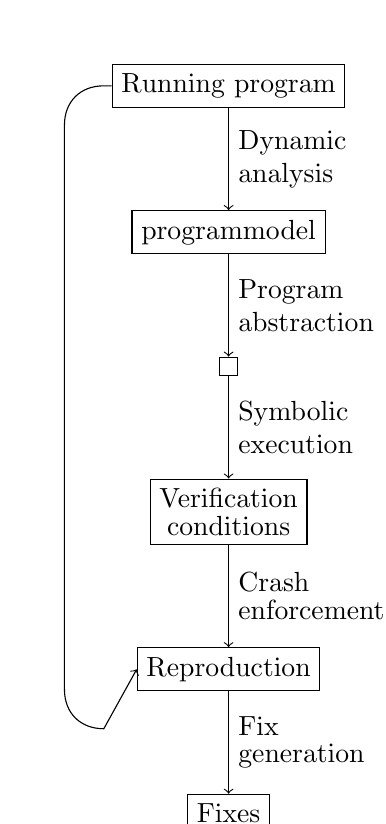
\begin{tikzpicture}
        [block/.style = {rectangle,draw,fill=white},
          node distance = 1.3]
        \node [block] (dynamic) {Running program};
        \node [block,below = of dynamic] (model) {\Gls{programmodel}};
        \node [block,below = of model] (statemachines) {\STateMachines};
        \node [block,below = of statemachines] (candidates) {\shortstack{Verification\\conditions}};
        \node [block,below = of candidates] (repro) {Reproduction};
        \node [block, below = of repro] (fix) {Fixes};
        \draw [->] (dynamic) to node [right] {\shortstack[l]{Dynamic\\analysis}} (model);
        \draw [->] (model) to node [right] {\shortstack[l]{Program\\abstraction}} (statemachines);
        \draw [->] (statemachines) to node [right] {\shortstack[l]{Symbolic\\execution}} (candidates);
        \draw [->] (candidates) to node [right] {\shortstack[l]{Crash\\enforcement}} (repro);
        \draw [->] (dynamic.west)
          -- ++(-.1,0)
          ..controls +(-0.3,0) and +(0, 0.3) .. ++(-0.5,-0.5)
          -- ++(0,-7.165)
          ..controls +(0,-0.3) and +(-0.3,0) .. ++( 0.5,-0.5)
          -- (repro.west);
        \draw [->] (repro) to node [right] {\shortstack[l]{Fix\\generation}} (fix);
      \end{tikzpicture}
    }
    \vspace{-4pt}
    \caption{System overview}
    \label{fig:basic_pipeline}
  \end{figgure}
  \vspace{-24pt}
\end{wrapfigure}
The basic approach is shown in \autoref{fig:basic_pipeline}.  The
process starts by observing the program's behaviour while operating
normally so as to build up a model of how it accesses memory.  This
model allows {\technique} to locate the parts of the program which are
most relevant to a particular concurrency error, and hence to build
\emph{\StateMachines} which more precisely model those areas.  These
     {\StateMachines} are then symbolically executed to determine
     whether running the modelled program fragments in parallel could
     lead to a concurrency error and, if so, to generate
     \glspl{verificationcondition} which precisely characterise the
     requirements for them to do so.  These
     \glspl{verificationcondition} are in turn used to construct
     co-programs which, when loaded into the running program, gently
     shepherd it towards these hypothesised bugs, allowing
     {\technique} to identify and discard any false positives with
     minimal manual intervention.  Any \glspl{verificationcondition}
     which survive this winnowing are then converted into binary
     patches which, when applied to the program, completely eliminate
     the bug.

All of these analyses and transformations are performed on the
program's machine code, with minimal (or in many non-trivial cases,
no) higher-level knowledge of the program's structure or environment.
This is in contrast to many previous systems, such as
Kivati~\cite{Chew2010} or AFix~\cite{Jin2011}, which operated on
either LLVM bitcode or the program's original source.  As such,
{\technique} can be applied to a wider class of programs, as it makes
no assumptions about the tools used to construct the program, and can
model the program's concurrency behaviour more accurately, as this
often depends on details of compiler optimisations which are visible
in machine code but not at higher levels.  On the other hand, the need
to infer information which other tools receive as input gives
{\technique} much higher computational cost, and this can limit its
applicability to more complicated bugs.  {\Technique} takes the
extreme position of attempting to analyse concurrency errors with
minimal support from the program, its environment, or its developers,
in some cases sacrificing practicality to do so.  As such, while it
can, as I demonstrate in the evaluation, often be usefully applied to
large software systems, such as MySQL or Thunderbird, it is perhaps
better thought of as an exploration of what can be achieved in an
unusually hostile analysis environment, and hence of the precise
trade-offs made when an analysis depends on richer input information,
rather than as a practical program maintenance technique in its own
right\editorial{That really isn't what I want to be saying.}.

\section{Contributions}

This dissertation makes several contributions:
\begin{itemize}
\item
  Suggest a novel method of finding and characterising
  concurrency-related bugs given only a binary program and some way of
  running it.
\item
  Describe how these characterisations can be used to automatically
  fix the bug or to make it more easily reproducible.
\item
  Evaluate the effectiveness and costs of these techniques with
  respect to a number of real and artificial test programs.
\end{itemize}
I give a detailed description of {\technique} and some results
obtained using \implementation, my prototype implementation.  These
include details of the fixes generated for a selection of bugs, both
artificial ones and some from real programs (including two which were
unknown to me before writing the tool), along with a demonstration
that the analysis scales to realistically large programs with
acceptable computational cost.  I also show that the fixes generated
typically have sufficiently low overhead to be useful in practice.

\section{Type of bug considered}
\label{sect:types_of_bugs}

{\Technique} considers only a subset of concurrency bugs: those where
one thread, referred to as the \gls{crashingthread}, is reading from a
shared data structure while another thread, the
\gls{interferingthread}, simultaneously modifies it, and these
concurrent updates cause the crashing thread to crash quickly.  In a
little more detail:
\begin{itemize}
\item The threads must be operating on a data structure located
  somewhere in shared memory.  This structure does not need to be in
  contiguous memory, and does not need to correspond to any
  higher-level concept of a data structure such as a C++
  \texttt{class} or \texttt{struct}, but it does need to be in
  process-accessible memory.  Structures on the filesystem, for
  instance, are not considered.
\item The \gls{crashingthread} must crash in a detectable way.  The
  simplest case is a hardware-detected fault such as referencing bad
  memory or dividing by zero, but more complex types of fault could
  also be supported, if a suitable detector can be implemented.
  {\Implementation} includes detectors for hardware-detected faults,
  assertion failures, and some types of double-free error.
\item The crash must be caused by the concurrent updates.  There must
  be some regions of the crashing and interfering threads such that
  running those regions in parallel can crash but running them
  atomically, in either order, will not.
\item The crashing thread must crash ``quickly''.  {\Technique} uses a
  finite \gls{analysiswindow} \gls{alpha} and will only consider
  reordering concurrent operations which occur at most \gls{alpha}
  instructions before the crash.  Bugs which require knowledge of the
  program behaviour beyond that window cannot be analysed.
  \gls{alpha} can, in principle, be arbitrarily large, but
  computational constraints mean that in practice it will be limited
  to a few dozen to a few hundred instructions, depending on the
  program to be analysed and how much information about the bug is
  available before analysis starts.
\end{itemize}
I refer to bugs which satisfy these constraints as \glslink{simple
  atomicity violation}{Simple Atomicity Violations}, or SAVs.  This
clearly does not include every possible type of concurrent bug (it
does not, for instance, include any but the most trivial deadlock
bugs, and complicated memory corruption bugs are difficult to handle),
but does include some interesting ones.

\begin{sanefig}
{\hfill}
\begin{tabular}{p{8cm}l}
Crashing thread:\hfill         & Interfering thread: \\
\\
1: Load $t_0$ from loc1        & 6: Load $t_3$ from loc1 \\
2: Store $t_0$ to loc2         & 7: Store $t_3$ to loc2 \\
\textit{Complicated local computation} & 8: Store $t_3 + 1$ to loc2 \\
3: Load $t_1$ from loc1        & \\
4: Load $t_2$ from loc2        & \\
5: Crash if $t_1 = t_2$ & \\
\end{tabular}
{\hfill}
\caption{An order violation bug. The complicated local computation
  does not modify loc1 or loc2.}
\label{fig:mandatory_concurrency1}
\end{sanefig}

\begin{sanefig}
\begin{centering}
\hfill
\begin{tabular}{p{8cm}l}
Crashing thread:          & Interfering thread: \\
\\
1: Load $t_0$ from loc1        & 6: Load $t_3$ from loc1 \\
2: Store $t_0+1$ to loc2       & 7: Store $t_3$ to loc2 \\
\textit{Complicated local computation} & 8: Store $t_3 + 1$ to loc2 \\
3: Load $t_1$ from loc1        & \\
4: Load $t_2$ from loc2        & \\
5: Crash if $t_1 = t_2$ & \\
\end{tabular}
\hfill
\end{centering}
\caption{Partial fix for the bug in
  \autoref{fig:mandatory_concurrency1}.}
\label{fig:mandatory_concurrency2}
\end{sanefig}

\subsection{Order-violation bugs}
The class of bugs described above does not include order violation
bugs, and so {\technique} will never report any.  Order violation bugs
in the program can, however, still sometimes affect the results.
Consider, for instance, the threads shown in
\autoref{fig:mandatory_concurrency1}.  These threads have an order
violation bug, in that the thread on the left will crash if it gets
from statement 2 to statement 3 before the thread on the right
executes.  Running the left-hand thread in isolation always leads to a
crash and so, within the definition used by {\technique}, this program
does not have a concurrency bug and no bug will be discovered,
reproduced, or fixed.

Suppose now that the ordering violation bug is fixed as shown in
\autoref{fig:mandatory_concurrency2}.  This program is ``more
correct'' than the previous one, in the sense that any instruction
interleaving which causes the new program to crash will also crash the
old one and some which crash the old will not crash the new, but
{\technique} \emph{will} report a potential bug in the new program.
Running the two new threads atomically, in either order, will never
crash, but interleaving them might (consider, for instance, the order
1, 2, 6, 7, 3, 4, 5).  The ordering violation bug effectively hid an
atomicity violation one, preventing {\technique} from finding either.

This non-monotonicity is an undesirable property for {\technique} to
have.  In practice, though, it is unlikely to be a serious problem.
Concurrency bugs in real programs tend to be at least moderately
difficult to reproduce, as easily reproduced bugs are generally fixed
quickly.  For this kind of bug, that implies that the local
computation must take time at least on the same order as operating
system scheduling effects, which usually range from a few tens of
microseconds to a few milliseconds.  On a modern process, that is
sufficient time to execute thousands to hundreds of thousands of
instructions, vastly exceeding {\technique}'s \gls{analysiswindow},
and so {\technique} is highly unlikely to capture an ordering
violation bug in the same window as an atomicity violation one.  If
two bugs are analysed in different windows then neither can hide the
other, and so there is little risk of an ordering violation disguising
an atomicity violation.

\subsection{Model of program execution}

In addition to restricting the class of bugs, {\technique} also
restricts the execution environment by assuming a strongly-ordered
memory model in which memory accesses are seen by all processors in
the order in which they appear in the program.  This is a reasonable
approximation for the widely-used x86 architecture, as that platform
rarely reorders memory accesses issued by a single
processor~\cite[Section 8.2]{Intel2009}.  Architectures with a weaker
memory ordering, such as Alpha~\cite[Section 5.6]{FFFCompaq2002} or
ARM~\cite[Section 5.3.4]{FFFARM2007}, would require more involved
processing to correctly capture the more complicated concurrency
semantics.

\section{Model of program modification}
\label{sect:intro:theory_of_fixing}

{\Technique} relies on being able to modify a program's behaviour in
order to reproduce and then to fix bugs, and aims to do so soundly, in
the sense that it should never introduce additional bugs.  This is not
entirely well-defined without access to a formal specification of the
program's desired behaviour.  It might be, for instance, that the
program is designed to investigate the possible ways in which a
particular processor can interleave memory accesses, and to report its
results by either exiting normally or crashing with an unhandled page
fault.  There is no general way for an automated tool to distinguish
such a program from one which is intended to always exit normally but
occasionally crashes due to an accidental race condition.  Any fix for
the latter would break the former.

{\Technique} defines a safe modification to a program to be one which
is equivalent to running it on a computer where some operations run
more slowly.  Equivalently, it will only ever introduce new bugs into
programs which depend on the relative timing of some operations.  This
is a reasonably conservative definition, in the sense that it allows
{\technique} to be applied to a reasonably broad variety of software,
but it is not quite universal.  In particular, {\technique} fixes and
\glspl{bugenforcer} can sometimes cause real-time programs to miss
their deadlines.  This is an inevitable risk when modifying a
program's scheduling without a precise specification of its deadline
structure, and, since {\technique} lacks such a specification, this is
the strongest safety property which can be hoped for.

\section{Graph generating grammars}
\label{sect:intro:graph_grammar}

\begin{sanefig}
  {\hfill}
  \tikzstyle{graphNT}+=[text width=1cm,fill=white]
  \begin{tabular}{lcclccrcc}
    \graphNT{$n$} & $\Rightarrow$ & \raisebox{-6mm}{\begin{tikzpicture}
        \node (n) {A};
        \node (nn) [style=graphNT, below=.5 of n] {$3n+1$};
        \draw[->] (n) -- (nn);
      \end{tikzpicture}} & \production{1} & \hspace{1cm} &
    \graphNT{2} & $\Rightarrow$ & \raisebox{-6mm}{
      \begin{tikzpicture}
        \node (2) {C};
        \node (1) [style = graphNT, below = .5 of 2] {1};
        \draw[->] (2) -- (1);
      \end{tikzpicture}
    } & \production{3} \\
    \graphNT{$m$} & $\Rightarrow$ & \raisebox{-6mm}{\begin{tikzpicture}
        \node (m) {B};
        \node (mm) [style=graphNT, below left =.5 of m] {$\frac{m}{2}$};
        \node (mmm) [style=graphNT, below right = .5 of m] {$\frac{m}{2} - 2$};
        \draw[->] (m) -- (mm);
        \draw[->] (m) -- (mmm);
    \end{tikzpicture}} & \production{2} & &
    \graphNT{4} & $\Rightarrow$ & \raisebox{-6mm}{
      \begin{tikzpicture}
        \node (4) {D};
        \node (2) [style=graphNT, below = .5 of 4] {2};
        \draw[->] (4) -- (2);
      \end{tikzpicture}
    } & \production{4} \\
  \end{tabular}
  {\hfill}
  \caption{Productions for the example graph generating grammar.  The
    terminals of this grammar are capital letters and the
    non-terminals are positive integers in boxes. $n$ matches odd
    integers and $m$ matches even integers other than two and four.
    Circled numbers are labels used to refer to the productions in the
    text.}
  \label{fig:intro:graph_grammar}
\end{sanefig}
\begin{sanefig}
  \newcommand{\arrowwidth}{0.03}
  \newcommand{\arrowhead}{0.05}
  \newcommand{\arrowlength}{0.8}
  \newcommand{\arrowdecoration}{}
  \newcommand{\labelledarrow}[1]{
    \hspace{-3.5mm}
    \begin{tikzpicture}
      \draw [\arrowdecoration] (0,-\arrowwidth) -- ++(\arrowlength,0);
      \draw [\arrowdecoration] (0,\arrowwidth) -- ++(\arrowlength,0);
      \draw [\arrowdecoration] (\arrowlength - \arrowhead + 0.01, 0 - \arrowwidth - \arrowhead) -- (\arrowlength + \arrowhead / 3 + \arrowwidth / 3, 0) -- (\arrowlength - \arrowhead + 0.01, \arrowwidth + \arrowhead);
      \node at (\arrowlength / 2,0) [above] {#1};
    \end{tikzpicture}\hspace{-3.5mm}
  }
  \tikzstyle{graphNT}+=[text width=1em, fill=white]
  \centerline{
  \begin{tikzpicture}[baseline=(r.base)]
    \node [style=graphNT] (r) {3};
  \end{tikzpicture}
  \labelledarrow{\production{1}}
  \begin{tikzpicture}[baseline=(r.base)]
    \node (r) {A\!\!};
    \node [left=-8pt of r] (r3) {\graphNT{3}:};
    \node [below = of r, style=graphNT] (s) {10};
    \draw[->] (r) -- (s);
  \end{tikzpicture}
  \labelledarrow{\production{2}}
  \begin{tikzpicture}[baseline=(r.base)]
    \node (r) {A\!\!};
    \node [left=-8pt of r] (r3) {\graphNT{3}:};
    \node [below=.57 of r] (s) {B\!\!};
    \node [left=-8pt of s] (r10) {\graphNT{10}:};
    \node [below=of s, style=graphNT] (t) {5};
    \draw[->] (r) -- (s);
    \draw[->] (s) -- (t);
    \draw[->] (s.east) .. controls +(.2,0) and +(0,-.2) .. ++(.33,.3) -- ++(0,0.55) .. controls +(0,.2) and +(.2,0) .. ++(-.3,.3) -- (r.east);
  \end{tikzpicture}
  \labelledarrow{\production{1}}
  \begin{tikzpicture}[baseline=(r.base)]
    \node (r) {A\!\!};
    \node [left=-8pt of r] (r3) {\graphNT{3}:};
    \node [below=.57 of r] (s) {B\!\!};
    \node [left=-8pt of s] (r10) {\graphNT{10}:};
    \node [below=.57 of s] (t) {A\!\!};
    \node [left=-8pt of t] (r10) {\graphNT{5}:};
    \node [below=of t,style=graphNT] (u) {16};
    \draw[->] (r) -- (s);
    \draw[->] (s) -- (t);
    \draw[->] (t) -- (u);
    \draw[->] (s.east) .. controls +(.2,0) and +(0,-.2) .. ++(.33,.3) -- ++(0,0.55) .. controls +(0,.2) and +(.2,0) .. ++(-.3,.3) -- (r.east);
  \end{tikzpicture}
  \labelledarrow{\production{2}}
  \begin{tikzpicture}[baseline=(r.base)]
    \node (r) {A\!\!};
    \node [left=-8pt of r] (r3) {\graphNT{3}:};
    \node [below=.57 of r] (s) {B\!\!};
    \node [left=-8pt of s] (r10) {\graphNT{10}:};
    \node [below=.57 of s] (t) {A\!\!};
    \node [left=-8pt of t] (r10) {\graphNT{5}:};
    \node [below=.57 of t] (u) {B\!\!};
    \node [left=-8pt of u] (r16) {\graphNT{16}:};
    \path (u.south) ++(-.7,-1) node [style=graphNT] (v) {8};
    \path (u.south) ++(.6,-1) node [style=graphNT] (w) {6};
    \draw[->] (r) -- (s);
    \draw[->] (s) -- (t);
    \draw[->] (t) -- (u);
    \draw[->] (u) -- (v);
    \draw[->] (u) -- (w);
    \draw[->] (s.east) .. controls +(.2,0) and +(0,-.2) .. ++(.33,.3) -- ++(0,0.55) .. controls +(0,.2) and +(.2,0) .. ++(-.3,.3) -- (r.east);
  \end{tikzpicture}
  \labelledarrow{\production{2}}
  \begin{tikzpicture}[baseline=(r.base)]
    \node (r) {A\!\!};
    \node [left=-8pt of r] (r3) {\graphNT{3}:};
    \node [below=.57 of r] (s) {B\!\!};
    \node [left=-8pt of s] (r10) {\graphNT{10}:};
    \node [below=.57 of s] (t) {A\!\!};
    \node [left=-8pt of t] (r10) {\graphNT{5}:};
    \node [below=.57 of t] (u) {B\!\!};
    \node [left=-8pt of u] (r16) {\graphNT{16}:};
    \path (u.south) ++(-.7,-.85) node [inner sep = 1.5 pt] (v) {B};
    \node [left=-7pt of v] (r8) {\graphNT{8}:};
    \path (v.south) ++(-.5,-1) node [style=graphNT] (x) {4};
    \path (v.south) ++(.5,-1) node [style=graphNT] (y) {2};
    \path (u.south) ++(.6,-1) node [style=graphNT] (w) {6};
    \draw[->] (r) -- (s);
    \draw[->] (s) -- (t);
    \draw[->] (t) -- (u);
    \draw[->] (u) -- (v);
    \draw[->] (u) -- (w);
    \draw[->] (v) -- (x);
    \draw[->] (v) -- (y);
    \draw[->] (s.east) .. controls +(.2,0) and +(0,-.2) .. ++(.33,.3) -- ++(0,0.55) .. controls +(0,.2) and +(.2,0) .. ++(-.3,.3) -- (r.east);
  \end{tikzpicture}
  }
  \centerline{
  \labelledarrow{$\cdots$}
  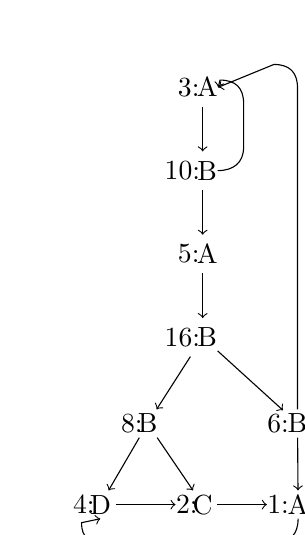
\begin{tikzpicture}[baseline=(r10.base)]
    \node (r) {A\!\!};
    \node [left=-8pt of r] (r3) {\graphNT{3}:};
    \node [below=.57 of r] (s) {B\!\!};
    \node [left=-8pt of s] (r10) {\graphNT{10}:};
    \node [below=.57 of s] (t) {A\!\!};
    \node [left=-8pt of t] (r10) {\graphNT{5}:};
    \node [below=.57 of t] (u) {B\!\!};
    \node [left=-8pt of u] (r16) {\graphNT{16}:};
    \path (u.south) ++(-.7,-.85) node [inner sep = 1.5 pt] (v) {B};
    \node [left=-7pt of v] (r8) {\graphNT{8}:};
    \path (v.south) ++(-.6,-.85) node [inner sep = 1.5pt] (x) {D};
    \node [left=-7pt of x] (r4) {\graphNT{4}:};
    \path (v.south) ++(.7,-.85) node [inner sep = 1.5pt] (y) {C};
    \node [left=-7pt of y] (r2) {\!\!\graphNT{2}:};
    \path (u.south) ++(.9,-.85) node (w) {\!\!\graphNT{6}:\!\!\!\!};
    \path (r2 -| w) node (z) {\!\!\graphNT{1}:\!\!\!\!};
    \node [right=1pt of z] [inner sep = 1.5pt] (z2) {A};
    \node [right=1pt of w] [inner sep = 1.5pt] (z3) {B};
    \draw[->] (r) -- (s);
    \draw[->] (s) -- (t);
    \draw[->] (t) -- (u);
    \draw[->] (u) -- (v);
    \draw[->] (u) -- (z3);
    \draw[->] (v) -- (x);
    \draw[->] (v) -- (y);
    \draw[->] (x) -- (r2);
    \draw[->] (y) -- (z);
    \draw[->] (z3) -- (z2);
    \draw[->] (s.east) .. controls +(.2,0) and +(0,-.2) .. ++(.33,.3) -- ++(0,0.55) .. controls +(0,.2) and +(.2,0) .. ++(-.3,.3) -- (r.east);
    \draw[->] (z2.south) .. controls +(0,-.2) and +(.2,0) .. ++(-.3,-.3) -- ++(-2.15,0) .. controls +(-.2,0) and +(0,-.2) .. ++(-.3,.25) -- (x.south);
    \draw[->] (z3.north) -- ++(0,4.08) .. controls +(0,.2) and +(.2,0) .. ++(-.3,.3) -- (r.east);
  \end{tikzpicture}
  \labelledarrow{}
  \begin{tikzpicture}[baseline=(r10.base)]
    \node (r) {\!\!A\!\!};
    \node [below=.57 of r] (s) {\!\!B\!\!};
    \node [below=.57 of s] (t) {\!\!A\!\!};
    \node [below=.57 of t] (u) {\!\!B\!\!};
    \path (u.south) ++(-.8,-.85) node [inner sep = 1.5 pt] (v) {B};
    \path (v.south) ++(-.55,-.85) node [inner sep = 1.5pt] (x) {D};
    \path (v.south) ++(.55,-.85) node [inner sep = 1.5pt] (y) {C};
    \path (u.south) ++(.8,-.85) node [inner sep = 1.5pt] (z3) {B};
    \path (y -| z3) node [inner sep = 1.5pt] (z2) {A};
    \draw[->] (r) -- (s);
    \draw[->] (s) -- (t);
    \draw[->] (t) -- (u);
    \draw[->] (u) -- (v);
    \draw[->] (u) -- (z3);
    \draw[->] (v) -- (x);
    \draw[->] (v) -- (y);
    \draw[->] (x) -- (y);
    \draw[->] (y) -- (z2);
    \draw[->] (z3) -- (z2);
    \draw[->] (s.east) .. controls +(.2,0) and +(0,-.2) .. ++(.33,.3) -- ++(0,0.55) .. controls +(0,.2) and +(.2,0) .. ++(-.3,.3) -- (r.east);
    \draw[->] (z2.south) .. controls +(0,-.2) and +(.2,0) .. ++(-.3,-.3) -- ++(-1.55,0) .. controls +(-.2,0) and +(0,-.2) .. ++(-.3,.25) -- (x.south);
    \draw[->] (z3.north) -- ++(0,4.08) .. controls +(0,.2) and +(.2,0) .. ++(-.3,.3) -- (r.east);
  \end{tikzpicture}
  }
  \caption[Expansion of a non-terminal using the productions in
    \autoref{fig:intro:graph_grammar}]{Expansion of the non-terminal
    \graphNT{$\mathrm{3}$} using the productions in
    \autoref{fig:intro:graph_grammar}.  Circled numbers above the
    arrows show which production was used at each step.}
  \label{fig:intro:graph_grammar:expansion}
\end{sanefig}

\noindent
Several of the algorithms in this dissertation are described in terms
of graph generating node-replacement grammars, and so I now give a
brief overview of this formalism using the example in
\autoref{fig:intro:graph_grammar}.  This figure shows a simple grammar
which produces directed graphs of (terminal) capital letters starting
from a single (non-terminal) integer.  The grammar works by matching a
pattern (on the left of the $\Rightarrow$) against some non-terminal
in the graph, possibly defining some match variables (in the example,
$n$ and $m$) in the process, generating a new fragment of graph (on
the right of the $\Rightarrow$), and replacing the original
non-terminal with the fragment.  This repeats until there are no more
non-terminals in the graph.  A non-terminal can only be generated at
most once; if a non-terminal is generated multiple times then it is
only added the first time and subsequent instances re-use the first
one.

\autoref{fig:intro:graph_grammar:expansion} shows how to apply this
grammar to the initial non-terminal \graphNT{3}.  The only production
that matches this initial graph is \production{1} with $n = 3$, which
generates a new terminal A with a single successor non-terminal
\graphNT{$3n+1$} = \graphNT{10}.  This non-terminal matches production
\production{2} with $m=10$, producing a terminal B and non-terminals
\graphNT{$\frac{m}{2}$}=\graphNT{5} and \graphNT{$\frac{m}{2}-2$} =
\graphNT{3}.  The \graphNT{3} non-terminal has already been generated
once, and so rather than adding a new node to the graph the grammar
adds an edge back to the previous one.  The grammar continues
expanding non-terminals in this way until none remain, producing the
graph at the bottom left of the figure.  The mapping from terminal
nodes to the non-terminals which generated them can then be forgotten,
producing the final graph at the bottom right of the figure.

\section{Structure of this dissertation}

This dissertation will, over the following chapters, present a
detailed description of how {\technique} works, starting with the
mechanism used to find and characterise bugs (\autoref{sect:derive})
and then moving on to describe how it first reproduces
(\autoref{sect:reproducing_bugs}) and then fixes
(\autoref{sect:fix_global_lock}) those bugs.  With the technique
itself described, I then give some experimental results obtained with
my prototype implementation {\implementation} (\autoref{chapter:eval})
and compare the technique to existing work in this area
(\autoref{chapter:related_work}).  Finally, I conclude and suggest
some possible avenues for future work (Chapters~\ref{sect:fw}
and~\ref{sect:concl}).


\chapter{Deriving and manipulating \StateMachines}
\label{chapter:derive_manip}
\section{Description of \StateMachines}
\label{sect:derive:description}

\todo{There's a pretty reasonable argument that this should be in the
  introduction.}

The core data structure used by {\technique} is the \StateMachine.
These consist of two main components: a
\introduction{summary}\editorial{Need a less generic-sounding name.}
of part of the program, in a simple (non-Turing complete) analysis
language, and an annotated fragment of the program's
\introduction{control flow graph (CFG)}, showing how states in the
\backref{summary} map to instructions in the program.

\backref{Summaries} themselves are acyclic graphs of
\introduction{analysis states}, which can be thought of as roughly
corresponding to possible points in the program's execution.  The
states themselves fall into one of four classes:

\begin{description}
\item[\introduction{Choice states}] These states have two successors
  and decide between them based on a condition, expressed as a
  \backref{BBDD}.  These states are used both to model the underlying
  program's control flow and also, by means of $\happensBeforeEdge$
  expressions, the possible interleavings of interacting threads.
\item[\introduction{Terminal states}] These states have no successors
  at all; if a \backref{summary} reaches one of these states it must
  terminate.  There are three \backref{terminal states}:

  \begin{description}
  \item \state{Crash}, which is used when the bug of interest
    reproduces.
  \item \state{Survive}, which is used when the bug of interest
    definitely does not reproduce.  Note that this does not
    necessarily indicate that the program is correct in any
    higher-level sense; it simply means that particular bug which is
    currently being investigated is not going to be triggered.
  \item \state{Unreached}, which is used to indicate that the rest of
    the analysis framework should ignore this path.  This can be used
    to prevent the analysis from considering certain uninteresting
    instruction interleavings.  It is also used if one of the
    intermediate analysis steps detects an inconsistency in the
    \backref{summary}, such as when reproducing the bug of interest
    requires the program to have suffered a fatal error earlier in its
    execution\editorial{Not quite what I want to say: inconsistency is
      within a path, but that example doesn't make that very clear.}.
  \end{description}
\item[\introduction{Side effect states}] These states have a single
  successor and represent the side-effects of program instructions,
  such as accessing memory or modifying registers.  The initial
  {\StateMachine} generated for a program fragment will usually have
  several \backref{side effect states} for each program instruction,
  especially on a CISC instruction set such as AMD64, but the various
  {\StateMachine} simplification passes will usually be able to
  eliminate most of these such that most program instructions have no
  \backref{side effect states} at all.  \backref{Side effect states}
  can also be used to update the {\StateMachine}'s own temporary
  variables (and in fact in a fully simplified {\StateMachine} the
  majority of \backref{side effect states} will update the
  {\StateMachine} temporaries rather than program registers).
\item[\introduction{Annotation states}] These states do not represent
  a change in the program's state, but instead represent a property
  which is guaranteed to be true if the {\StateMachine} reaches that
  \backref{analysis state}.  Examples of such properties include the
  layout of a particular thread's stack or the aliasing configuration
  of certain registers.  These states are mostly derived from the
  program model, and are used to integrate the results of the initial
  \backref{static} and \backref{dynamic analysis phases} into the
  {\StateMachines}.
\end{description}

The \backref{CFG} component of the {\StateMachine} is used to map
\backref{analysis states} back to instructions in the original
program.  In particular, it shows how loops in the original program
were unrolled, where control-flow edges had to be removed in order to
make the \backref{summary} acyclic, and where the \backref{summary}
crosses function boundaries.  This is necessary to relate properties
of the {\StateMachines}, such as the \backref{verification conditions}
of \backref{candidate bugs}, back to the behaviour of the original
program, which is necessary to generate \backref{bug enforcers} and
\backref{fixes}.  For multi-threaded {\StateMachines}, there will be
one \backref{CFG} for each thread.\editorial{Doesn't really say what
  the CFGs \emph{are}.}

\begin{figure}
\begin{verbatim}
400694: mov    global_ptr,%rax
40069b: test   %rax,%rax
40069e: je     4006ad
4006a0: mov    global_ptr,%rax
4006a7: movl   $0x5,(%rax)
\end{verbatim}
\caption{A fragment of machine code.  The {\StateMachine} for this fragment is shown in Figure~\ref{fig:derive:single_threaded_machine}}
\label{fig:derive:single_threaded_machine_inp}
\end{figure}

\begin{figure}
  \begin{minipage}{35mm}
    \begin{subfloat}
      \begin{tikzpicture}
        \node (cfg6) at (0,2) [CfgInstr] {cfg6:400694};
        \node (cfg5) [CfgInstr, below=of cfg6] {cfg5:40069b};
        \node (cfg4) [CfgInstr, below=of cfg5] {cfg4:40069e};
        \node (cfg3) [CfgInstr, below=of cfg4] {cfg3:4006a0};
        \draw[->] (cfg6) -- (cfg5);
        \draw[->] (cfg5) -- (cfg4);
        \draw[->] (cfg4) -- (cfg3);
      \end{tikzpicture}
      \caption{\backref{CFG} fragment}
    \end{subfloat}
  \end{minipage}
  \begin{subfloat}
    \begin{minipage}{70mm}
      \begin{tikzpicture}
        \node (l1) at (0,2) [stateSideEffect] {l1: \state{Load} tmp1 $\leftarrow$ global\_ptr AT cfg6 };
        \node (l2) [stateIf, below=of l1] {l2: \state{If} (0 == tmp1)};
        \node (l4) [stateSideEffect, below=of l2] {l4: \state{Load} tmp2 $\leftarrow$ global\_ptr AT cfg3 };
        \node (l3) [stateTerminal, right=of l4] {l3: \state{Survive} };
        \node (l5) [stateIf, below=of l4] {l5: \state{If} (BadPtr(tmp2))};
        \node (l6) [stateTerminal, below=of l5] {l6: \state{Crash}};
        \draw[->] (l1) -- (l2);
        \draw[->,ifTrue] (l2) -- (l3);
        \draw[->,ifFalse] (l2) -- (l4);
        \draw[->] (l4) -- (l5);
        \draw[->,ifFalse] (l5) -- (l3);
        \draw[->,ifTrue] (l5) -- (l6);
      \end{tikzpicture}
    \end{minipage}
    \caption{Program \backref{summary}}
  \end{subfloat}
  \caption{{\StateMachine} generated from the machine code in
    Figure~\ref{fig:derive:single_threaded_machine_inp}, assuming that
    the bug to be investigated is a crash at 4006a7.  Dotted lines
    leaving an \state{If} state indicate the false branch; solid ones
    indicate the true branch.}\smh{Captions in italics?}
  \label{fig:derive:single_threaded_machine}
\end{figure}

Figure~\ref{fig:derive:single_threaded_machine} shows an example of a
simple single-threaded \StateMachine\footnote{This is the read-side of
  the simple\_toctou test discussed in more detail in
  \S\ref{sect:eval:art:simple_toctou}.}.  It illustrates a simple
time-of-check, time-of-use race: the program loads from
\verb|global_ptr| twice in quick succession, validating the result of
the first and using the result of the second.  The translation to a
{\StateMachine} is hopefully reasonably clear: the \backref{CFG} on
the left covers all of the relevant instructions and the
\backref{summary} on the right expresses the relevant part of their
behaviour.  It is trivial to read off from these diagrams that the
program might crash if some other thread modifies \verb|global_ptr| in
between the two loads and will otherwise survive.  Notice that
\verb|4006a7|, the instruction which crashes, is not itself
represented in the \backref{CFG}: by the time that instruction
executes, the program is either doomed to crash or has definitely
avoided the bug, and so that instruction is irrelevant to determining
when (and whether) the bug can actually happen, and so it is not
included in the {\StateMachine}.

\begin{figure}[t]
\begin{verbatim}
4008fb: movq   $0x0,global_ptr
\end{verbatim}
\caption{Other side of the racing code shown in Figure~\ref{fig:derive:single_threaded_machine_inp}.}
\label{fig:derive:single_threaded_machine_write_inp}
\end{figure}

\begin{figure}[t]
  \begin{minipage}{50mm}
    \begin{subfloat}
      \begin{tikzpicture}
        \path (0,0mm) -- (3cm, 0cm);
        \node (cfg8) at (0,0) [CfgInstr] {cfg8:4008fb};
      \end{tikzpicture}
      \vspace{-20mm}\caption{\backref{CFG} fragment}
    \end{subfloat}
  \end{minipage}
  \begin{subfloat}
    \begin{minipage}{70mm}
      \begin{tikzpicture}
        \node (l7) [stateSideEffect] {l7: \state{Store} 0 $\rightarrow$ global\_ptr AT cfg8 };
      \end{tikzpicture}
    \end{minipage}
    \caption{Program \backref{summary}}
  \end{subfloat}
  \caption{{\STateMachine} generated from the code in
    Figure~\ref{fig:derive:single_threaded_machine_write_inp}.  In
    this case, the code to be represented has only a single
    instruction, and so the {\StateMachine} is very
    simple.}\todo{Looks a bit silly.}
  \label{fig:derive:single_threaded_machine_write}
\end{figure}

\begin{sidewaysfigure}
  \begin{tikzpicture}
    \node (lA) [stateIf] { \state{If} $\happensBefore{\mai{cfg6}{thread1}}{\mai{cfg8}{thread2}}$ };
    \node (lB) [stateSideEffect, below = of lA] { l1: \state{Load} tmp1 $\leftarrow$ global\_ptr AT cfg6:thread1 };
    \node (lC) [stateSideEffect, below right = of lA] {l7: \state{Store} 0 $\rightarrow$ global\_ptr AT cfg8:thread2 };
    \node (lD) [stateIf, below = of lB] { l2: \state{If} (0 == tmp1) };
    \node (lE) [stateTerminal, below = of lC] { \state{Unreached} };
    \node (lF) [stateIf, below left = of lD] {\state{If} $\happensBefore{\mai{cfg3}{thread1}}{\mai{cfg8}\mai{thread2}}$ };
    \node (lG) [stateTerminal, below right = of lD] {\state{Survive}};
    \node (lH) [stateTerminal, below right = of lF] {\state{Unreached}};
    \node (lI) [stateSideEffect, below = of lF] {l7: \state{Store} 0 $\rightarrow$ global\_ptr AT cfg8:thread2 };
    \node (lJ) [stateSideEffect, below = of lI] {l4: \state{Load} tmp2 $\leftarrow$ global\_ptr AT cfg3:thread1 };
    \node (lK) [stateIf, below = of lJ] { l5: \state{If} $BadPtr(tmp2)$ };
    \node (lL) [stateTerminal, below left = of lK] { \state{Crash} };
    \node (lM) [stateTerminal, below right = of lK] { \state{Survive} };
    \draw[->,ifTrue] (lA) -- (lB);
    \draw[->,ifFalse,draw] (lA) -- (lC);
    \draw[->] (lB) -- (lD);
    \draw[->] (lC) -- (lE);
    \draw[->,ifTrue] (lD) -- (lG);
    \draw[->,ifFalse] (lD) -- (lF);
    \draw[->,ifTrue] (lF) -- (lH);
    \draw[->,ifFalse] (lF) -- (lI);
    \draw[->] (lI) -- (lJ);
    \draw[->] (lJ) -- (lK);
    \draw[->,ifTrue] (lK) -- (lL);
    \draw[->,ifFalse] (lK) -- (lM);
  \end{tikzpicture}
  \caption{\backref{Summary} component of the cross-product of the
    {\StateMachine} shown in
    figures~\ref{fig:derive:single_threaded_machine} and
    \ref{fig:derive:single_threaded_machine_write}.  The \backref{CFG}
    component just contains the fragments from the two input
    {\StateMachines}.}
  \label{fig:derive:cross_thread}
\end{sidewaysfigure}

\begin{figure}
  \begin{tikzpicture}
    \node (lA) [stateSideEffect] {\state{Assert} $0 \not= InitMemory(global\_ptr)$ and $cfg6:thread1 \happensBefore cfg7:thread2$};
    \node (lB) [stateIf, below = of lA] {\state{If} $cfg3:thread1 \happensBefore cfg7:thread2$ };
    \node (lC) [stateTerminal, below left = of lB] {\state{Survive}};
    \node (lD) [stateTerminal, below right = of lB] {\state{Crash}};
    \draw [->] (lA) -- (lB);
    \draw [->,ifTrue] (lB) -- (lC);
    \draw [->,ifFalse] (lB) -- (lD);
  \end{tikzpicture}
  \caption{\STateMachine from figure~\ref{fig:derive:cross_thread}
    after {\StateMachine} simplification.}
  \label{fig:derive:cross_thread_opt}
\end{figure}

\STateMachines become somewhat more interesting when they capture the
results of multiple threads.  Figure~\ref{fig:derive:cross_thread}
shows an example of a \introduction{cross-product \StateMachine},
which captures all of the interleavings of the two input
{\StateMachines} which the analysis needs to consider.  There are a
couple of interesting new features here:

\begin{itemize}
\item Several new states have been created and existing ones
  duplicated.  In particular, some memory accesses have now been
  duplicated to multiple places in the \StateMachine.
\item
  $\happensBeforeEdge$ expressions.  These allow the {\StateMachine}
  to query the program's happens-before graph.
  $\happensBefore{\mai{cfgA}{threadB}}{\mai{cfgC}{threadD}}$ is true
  precisely when memory access $A$ in thread $B$ happens before memory
  access $C$ in thread $D$.  These memory accesses will usually
  correspond to specific instructions in the program, but this is not
  guaranteed.

  \todo{Actual implementation has another layer of indirection here,
    so that CFG nodes don't need to match up precisely with memory
    accesses, which is useful if one instruction makes multiple
    accesses or if we decide to merge multiple program accesses into
    one summary-level access.  I'm optimistic that I'll be able to get
    away without explaining that, though.}
\item
  Paths in which either the read or write \backref{summary} finish
  without the other starting will end in an unreached state, so they
  will not be considered by the later analysis phases.  Although not
  apparent in this simple example, the algorithm used by SLI also uses
  partial-order reduction\needCite{} to further reduce the number of
  interleavings to be considered\editorial{Need to be more precise
    about that.}.
\end{itemize}

The {\StateMachine} shown in Figure~\ref{fig:derive:cross_thread}
correctly captures the interaction of the two input {\StateMachines}
but is more complicated than it needs to be.  {\Technique} therefore
performs a few simplifications on the \StateMachine, detailed later,
before passing the {\StateMachine} to the symbolic execution engine;
the results are shown in Figure~\ref{fig:derive:cross_thread_opt}.

\STateMachines have a couple of other features not shown in this
example:

\begin{itemize}
\item
  \introduction{Control-flow expressions}.  Much as {\StateMachines}
  can query the happens-before graph of a program using
  $\happensBeforeEdge$ expressions, they can also query the control
  flow within a given thread using $\mathrm{Entry}$ and
  $\mathrm{ControlFlow}$ expressions.  An
  $\entryExpr{\mai{threadA}{cfgB}}$ expression is true if thread $A$
  entered its \backref{CFG} fragment at $\mathrm{cfgB}$, while
  $\controlEdge{threadA}{cfgB}{cfgC}$ is true if thread $A$
  transitions from \backref{CFG} node $B$ to node $C$.  Note that the
  value of $\mathrm{Control}$ expression does not depend on where in
  the {\StateMachine} it is evaluated: the control flow within a
  {\StateMachine} is (conceptually) independent of that of the
  original program.
\item
  $\Phi$ side-effects.  These are described later when discussing the
  SSA form used; they have somewhat different semantics from the
  $\Phi$ nodes used in optimising compilers.
\item
  \state{StartAtomic} and \state{EndAtomic} side-effects.  These
  indicate that a given fragment of the {\StateMachine} should execute
  atomically, and hence restrict the cross-product
  {\StateMachine}\smh{This is a nice concept, wonder if it needs a
    better name?}.  They are used both to represent instructions with
  the \verb|LOCK| prefix (which execute atomically) and some
  library-level functions such as
  \verb|pthread_mutex_lock|\editorial{Should probably have a forwards
    ref to discussion of handling library functions.}.
\item
  Initial-memory expressions, written $LD(addr)$.  {\STateMachines}
  can always access the contents of memory as it was when the
  {\StateMachine} started, ignoring any subsequent updates.  It is
  often easier to analyse conditions expressed in terms of these
  expressions than equivalent conditions expressed in terms of
  explicit memory-accessing operations, and the results are usually
  easier to understand.

  Note that the address part of the expression is evaluated against
  the \emph{current} state of the {\StateMachine}, and can therefore
  reference {\StateMachine} variables and so forth, even though the
  load itself is evaluated against a snapshot of the program's initial
  memory.\smh{Hmm -- seems complicated/arbitrary -- why?  Can you
    clarify?}
\end{itemize}

\section{Deriving \StateMachines}
\label{sect:derive:derive}

\todo{This is much bigger than I would like, given that it's not
  actually all that interesting.}

The way in which {\StateMachines} are built depends on how much
information is available before the analysis starts.  The simplest
case is that only the instruction pointer for the instruction which
crashed is available, and so I discuss that case first.  I then go on
to describe how to generalise this algorithm to operate when no
information is available at all, such as when trying to discover a
currently-unknown bug (Section~\ref{sect:derive:unknown_bugs}), and
when more information is available about the program's state at the
time of the crash (Section~\ref{sect:derive:from_core_dump}).

\todo{I'm not convinced that this is a good way of discussing this,
  because those generalisations are pretty obvious and this is
  building them up to be a little more clever than they really are.
  On the other hand, it does make the description of the main
  algorithm a bit clearer.}

\subsection{Building the read thread's \StateMachine}

The input to this phase of the analysis is the raw instruction pointer
for the thread which crashed, at the time of the crash, plus the
program binary and \backref{program model}.  It must use these to
build a {\StateMachine} representing the final \backref{$\alpha$}
instructions executed by the read thread.  The approach used has
several stages:

\begin{itemize}
\item First, determine which instructions need to be included in the
  {\StateMachine}.  This will be a fragment of the program's control
  flow graph which includes every instruction which the crashing
  thread might have executed in the \backref{$\alpha$} instructions
  immediately prior to crashing, and as few other instructions as
  possible.  This is described in more detail in
  Section~\ref{sect:derive:build_static_cfg}.
\item Next, unroll any loops in that control flow graph fragment such
  that all cyclic paths contain at least \backref{$\alpha$}
  instructions.  At that point, the cycles can be safely broken
  without changing the program's behaviour within the
  \backref{analysis window}.  This unrolled, acyclic CFG forms the
  \backref{CFG} component of the {\StateMachine}.  This is described
  in more detail in Section~\ref{sect:derive:handling_loops}.
\item The acyclic \backref{CFG} can then be compiled to produce the
  initial \backref{summary} component of the {\StateMachine}.  Each
  instruction in the \backref{CFG} is translated independently and the
  resulting fragments are then stitched back together to form the
  \backref{summary}.  This is described in
  Section~\ref{sect:derive:compile_cfg}.
\item The \backref{summary} is then compared to the \backref{program
  model}, producing \backref{annotation states} as necessary.
  Detailed discussion of how these annotations are generated is
  deferred to Section~\ref{sect:alias_analysis}, which also describes
  the main consumer of them.
\item Finally, the \backref{summary} is converted to
  \introduction{static single assignment} form (SSA).  The SSA form
  used by {\technique} is described in Section~\ref{sect:ssa}.
\end{itemize}

The resulting {\StateMachine} captures all of the relevant information
from this thread and can be consumed by the rest of the analysis
framework.

\subsection{Building the read thread's static control-flow graph}
\label{sect:derive:build_static_cfg}
The first stage, once a potentially-crashing instruction has been
selected for investigation, is to build a static control-flow graph
containing all of the instructions which might appear in the
\backref{analysis window}.  This is done by starting with a trivial
CFG containing just the crashing instruction and then expanding it
backwards, one instruction at a time, until every needed instruction
has been discovered.

\begin{figure}
\begin{algorithmic}[1]
\State $depth \gets 0$
\State $pendingAtDepth \gets \queue{targetInstrAddress}$
\State $result \gets \map{}$
\While{$depth < \alpha$}
  \State $pendingAtNextDepth \gets \queue{}$
  \While{$\neg{}empty(pendingAtDepth)$}
    \State $currentInstr \gets pop(pendingAtDepth)$
    \If {$result \textrm{ has entry for } currentInstr$}
      \State \textbf{continue}
    \EndIf
    \State $current \gets \text{decode instruction at } currentInstr$
    \State $\mapIndex{result}{currentInstr} \gets current$
    \State $predecessors \gets \text{predecessors of } currentInstr$\smh{How do we compute predecessors?}
    \State Add $predecessors$ to $pendingAtNextDepth$
  \EndWhile
  \State $pendingAtDepth \gets pendingAtNextDepth$
  \State $depth \gets depth + 1$
\EndWhile
\end{algorithmic}
\caption{Building a read-side static control flow graph within a
  single function.  Computing the predecessors of an instruction is
  non-trivial and is discussed in more detail in the text below.}
\label{fig:derive:static_read_cfg_single_function}
\end{figure}

The simple case is that all of the needed instructions are contained
within a single function.  In that case, the algorithm is as shown in
Figure~\ref{fig:derive:static_read_cfg_single_function}.  This simply
implements a depth-limited breadth-first search starting at the
potentially-crashing instruction and exploring backwards through the
program's control flow.  Note that this can result in a CFG with
multiple roots.

There is a slight subtlety on line 13, which determines the
predecessors of a given instruction.  This is not always obvious,
given only a binary program, for three reasons:

\begin{itemize}
\item
  The program might contain indirect branches.  It is difficult to
  determine statically where these might branch to.  A conservative
  approach would be to assume that they might branch anywhere, but
  this leads to unmanageably complex CFGs even for trivial programs.
  At the same time, ignoring them completely means that many important
  program paths will be missed.
\item
  Many instruction sets include variable-length instructions, and so
  there might be several overlapping instructions which all finish at
  the start of the instruction currently being investigated.  In most
  programs, only one of these will ever be executed, and it is
  important to pick the right one.
\item
  It is not always possible to identify which parts of a program are
  instructions and which data, which makes it difficult to determine
  whether a given sequence of bytes which happens to have the right
  format to be a branch instruction should be treated as one.
\end{itemize}

{\Implementation} solves this problem using a combination of
\backref{static} and \backref{dynamic analysis}.  First, the
\backref{dynamic analysis} tracks the targets of all indirect branch
and call instructions.  This makes the first problem trivial (assuming
that the dynamic analysis is complete).  This information also
includes a list of all of the functions in the program which are
called by the operating system or by library functions\footnote{Shared
  libraries, in the usual model, cannot statically assume anything
  about the memory layout of the program which they are to be linked
  against, and so all branches from a shared library into the main
  program will be indirect.}.  Knowing all entry points into the main
program, plus all branches within the main program, is sufficient for
a simple static analysis to enumerate every instruction in the main
program, and this then allows the second and third problems to be
solved as well.\editorial{I want to mention the \backref{program
    model} in there somewhere, but can't quite fit it in.}

\todo{But that doesn't quite work for types of run-time generated code
  other than shared libraries.  Might need to say something about
  that.}\smh{Hmm -- perhaps .. (this would matter e.g. for obfuscated
  code like burnintest)... But maybe could defer to end f the
  section/or chapter or dissertation?}

\subsection{Handling loops in the read thread's CFG}
\label{sect:derive:handling_loops}

There may be loops in the CFGs generated by the algorithm in
Section~\ref{sect:derive:build_static_cfg}, but {\technique} requires
that the {\StateMachines} be finite and acyclic.  These loops must
therefore be eliminated, and they must be eliminated in a way which is
guaranteed to preserve all paths of length \backref{$\alpha$} ending
at the instruction being investigated.  The approach {\technique}
takes is to unroll the loops, duplicating instructions as necessary,
until every path from a root of the CFG to the target instruction is
either free from cycles or of length greater than \backref{$\alpha$}.
The remaining cycles can then be eliminated without changing the
program's behaviour within the \backref{analysis window}.

\begin{figure}
\begin{tikzpicture}
  [node distance=1 and 0.3]
  \begin{scope}
    \node (A) at (0,2) [CfgInstr] {A};
    \node (B) [CfgInstr] [below=of A] {B}; 
    \node (C) [CfgInstr] [below=of B] {C}; 
    \node (D) [CfgInstr] [below=of C] {D}; 
    \draw[->] (A) -- (B);
    \draw[->] (B) -- (C);
    \draw[->] (C) -- (D);
    \draw[->] (C.east) to [bend right=90] (B.east) node (edge1) [right] {};
    \begin{pgfonlayer}{bg}
      \node (box1) [fill=black!10,fit=(A) (B) (C) (D) (edge1)] {};
    \end{pgfonlayer}
  \end{scope}
  \begin{scope}[xshift=4cm]
    \node (A) at (0,2) [CfgInstr] {A};
    \node (B) [CfgInstr] [below=of A] {B}; 
    \node (C) [CfgInstr] [below=of B] {C}; 
    \node (D) [CfgInstr] [below=of C] {D};  
    \node (C') [CfgInstr] [right=of C] {C'};
    \draw[->] (A) -- (B);
    \draw[->] (B) -- (C);
    \draw[->] (C) -- (D);
    \draw[->] (B) to [bend right=10] (C');
    \draw[->] (C') to [bend right=10] (B);
    \begin{pgfonlayer}{bg}
      \node (box2) [fill=black!10,fit=(A) (B) (C) (D) (C')] {};
    \end{pgfonlayer}
  \end{scope}
  \begin{scope}[xshift=8cm]
    \node (A) at (0,2) [CfgInstr] {A};
    \node (B) [CfgInstr] [below=of A] {B};
    \node (B') [CfgInstr] [right=of B] {B'};
    \node (C) [CfgInstr] [below=of B] {C};
    \node (D) [CfgInstr] [below=of C] {D};
    \node (C') [CfgInstr] [right=of C] {C'};
    \draw[->] (A) -- (B);
    \draw[->] (B) -- (C);
    \draw[->] (C) -- (D);
    \draw[->] (C') -- (B);
    \draw[->] (A) -- (B');
    \draw[->] (B') to [bend right=10] (C');
    \draw[->] (C') to [bend right=10] (B');
    \begin{pgfonlayer}{bg}
      \node (box3) [fill=black!10,fit=(A) (B) (C) (D) (C') (B')] {};
    \end{pgfonlayer}
  \end{scope}
  \begin{scope}[xshift=12cm]
    \node (A) at (0,2) [CfgInstr] {A};
    \node (B) [CfgInstr] [below=of A] {B};
    \node (B') [CfgInstr] [right=of B] {B'};
    \node (C) [CfgInstr] [below=of B] {C};
    \node (C') [CfgInstr] [right=of C] {C'};
    \node (C'') [CfgInstr] [right=of C'] {C''};
    \node (D) [CfgInstr] [below=of C] {D};
    \draw[->] (A) -- (B);
    \draw[->] (B) -- (C);
    \draw[->] (C) -- (D);
    \draw[->] (C') -- (B);
    \draw[->] (A) -- (B');
    \draw[->] (B') -- (C');
    \draw[->] (C'') to [bend right=10] (B');
    \draw[->] (B') to [bend right=10] (C'');
    \begin{pgfonlayer}{bg}
      \node (box4) [fill=black!10,fit=(A) (B) (C) (D) (C') (B') (C'')] {};
    \end{pgfonlayer}
  \end{scope}
  \draw[->,thick] (box1) -- (box2) node [above,midway] {duplicate C};
  \draw[->,thick] (box2) -- (box3) node [above,midway] {duplicate B};
  \draw[->,thick] (box3) -- (box4) node [above,midway] {duplicate C'};
  \draw[->,thick] (box4) -- +(2.5,0) node [above,midway] {...};
\end{tikzpicture}
\caption{A CFG containing a cycle.}
\label{fig:cyclic_cfg}
\end{figure}

\begin{figure}
\begin{center}
\begin{tikzpicture}
  [node distance=1 and 0.3]
  \node (A) at (0,2) [CfgInstr] {A};
  \node (B) [CfgInstr] [below=of A] {B};
  \node (B') [CfgInstr] [right=of B] {B'};
  \node (C) [CfgInstr] [below=of B] {C};
  \node (C') [CfgInstr] [right=of C] {C'};
  \node (C'') [CfgInstr] [above right=of B'] {C''};
  \node (D) [CfgInstr] [below=of C] {D};
  \draw[->] (A) -- (B);
  \draw[->] (B) -- (C);
  \draw[->] (C) -- (D);
  \draw[->] (C') -- (B);
  \draw[->] (A) -- (B');
  \draw[->] (B') -- (C');
  \draw[->] (C'') -- (B');
  \begin{pgfonlayer}{bg}
    \node (box4) [fill=black!10,fit=(A) (B) (C) (D) (C') (B') (C'')] {};
  \end{pgfonlayer}\smh{Center?}
\end{tikzpicture}
\end{center}
\caption{Fully unrolled version of the CFG in
  Figure~\ref{fig:cyclic_cfg}, preserving all paths of length six or
  fewer instructions.  Note that an additional root has been
  introduced at C''.}\todo{Underful hbox}
\label{fig:unrolled_cyclic_cfg}
\end{figure}

As an example, consider the CFG shown at the left of
Figure~\ref{fig:cyclic_cfg}, which contains a loop between
instructions B and C.  This loop must be removed from the CFG while
maintaining all paths which terminate at D and which contain
\backref{$\alpha$} or fewer instructions.  The algorithm starts by
performing a depth-first traversal backwards through the graph from D
until it finds an edge which closes a cycle.  In this case, that is
the edge from C to B.  SLI will therefore break this edge by
duplicating the instruction at the start of the edge, C, along with
all of its incoming edges (in this case, just the B to C edge).  The C
to B edge can then be redirected to be from C' to B, producing the
next diagram in the sequence.  All paths which were possible in the
old graph will also be possible in the new one, if duplicated nodes
are treated as semantically equivalent, and the loop is now one
instruction further away from the target instruction D.  The process
then repeats, moving the cycle steadily further and further away from
D until all paths ending of length \backref{$\alpha$} ending at D are
acyclic, at which point the cycle can be safely removed from the
graph.

Note that the edge which is modified is the back edge, from C to B,
which points ``away from D'', and not the forwards edge from B to C.
Trying to break the B to C edge would have moved the cycle away from A
rather than away from D, which would not be helpful.

\begin{figure}
\begin{algorithmic}[1]
  \While {graph is not cycle-free}
     \State $edge \gets \textsc{findEdgeToBeBroken}(targetInstr)$
     \If {$edge$ is at least $N_r$ instructions from target instruction}
        \State {Erase $edge$ from graph}
     \Else
        \State {$newNode \gets$ duplicate of $edge.source$}
        \For {$i$ incoming edge of $edge.source$}
           \State {Create a new edge from $i.source$ to $newNode$}
        \EndFor
        \State {Replace $edge$ with an edge from $newNode$ to $edge.destination$}
     \EndIf
  \EndWhile
\end{algorithmic}
\caption{Loop unrolling and cycle breaking algorithm.
  \textsc{findEdgeToBeBroken} simply performs a depth-first search of
  the graph backwards from $targetInstr$ and returns the first edge
  which completes a cycle.}
\label{fig:derive:read:unroll_cycle_break}
\end{figure}

The complete algorithm is shown in
Figure~\ref{fig:derive:read:unroll_cycle_break}.  This algorithm is
guaranteed to preserve all paths of length $N_r$ which end at the
target instruction.  There are only two places in the algorithm which
remove existing edges, so consider each in turn.  The first is the
erasure on line 4.  This can only ever affect edges whose shortest
path to a target is at least $N_r$ instructions long, and so cannot
eliminate any paths to a target of length $N_r$, and is therefore
safe.  The other is the replacement step at line 10, which replaces an
edge from $edge.source$ to $edge.destination$ with one from $newNode$
to $edge.destination$.  This is safe provided that every path to
$newNode$ has a matching path to $edge.source$, which is ensured by
duplicating all of $edge.source$'s incoming edges to $newNode$.  At
the same time, no additional paths will be introduced, because every
path to $newNode$ has a matching path to $edge.source$.

\todo{Is it worth doing a proof of termination as well?}\smh{No,
  although you might comment on the expected running time...}

\subsection{Handling cross-function CFGs.}

\label{sect:derive:cross_function_cfgs}

There is, of course, no guarantee that all of the instructions in the
\backref{analysis window} will be contained within a single function,
and if they are not then {\technique} must be able to generate
appropriate cross-function \backref{CFG}s.  It does so by partially
inlining functions as necessary to restore the problem to the
single-function case.  This means that instructions must be labelled
by both the pointer of the instruction itself and also by its inlining
context, which is simply the stack of functions into which it has been
inlined\editorial{Not terribly clear.}.  The only slight complications
are that the inlining context is not necessarily known when CFG
exploration starts, and it might be necessary to consider the same
instruction in several contexts.

\todo{That's kind of a stupid way of doing this.  Should only need to
  duplicate instructions when the inlining context matters, which is
  pretty much just when we see both the start and end of the
  function.}

There are two important cases to consider: backing into another
function, where the exploration starts in one function and must be
extended backwards into the end of another one, and backing out of
one, where the exploration starts in one function and must be extended
to include that function's callers.  Backing into a function is
simple: the analysis finds the functions which are to be
called\footnote{There might be more than one function if the
  instruction is a dynamic call.  In that case, the \backref{program
    model} is used to find the set of all possibly-called functions
  and they are all treated as possible predecessors.}, finds all of
the return instructions in those functions, and treats those as the
predecessor of the current instruction with an appropriately extended
inlining context.

Backing out of a function is more complex.  In this case, the analysis
must consider all possible callers of the target function and inline
the target function into each.  

\todo{As I write this I realise that the way I've done this is really,
  really stupid.  I should probably fix that before writing any more
  about it.}\smh{An example or two would probably help, too.}

Tail calls do not require any particular special handling here.  If
the exploration reaches the start of a function then all branches to
that instruction will be treated as possible predecessors of it,
regardless of whether they come from call instructions or simple
branch instructions.

\subsection{Compiling the CFG to a \StateMachine}
\label{sect:derive:compile_cfg}

\todo{Should mention that I use libVEX\smh{probably not at this level
    of abstraction.} to convert instructions to a slightly saner
  intermediate format before converting to {\StateMachine} fragments,
  rather than doing it directly.}

The algorithm presented so far can build the \backref{CFG} component
of the {\StateMachine}.  The next step is to convert that
\backref{CFG} into the \backref{summary} component.  The
{\StateMachine} analysis language is powerful enough to make
translating individual instructions in isolation completely
straightforward.  Connecting them together is, however,
slightly more difficult, as the edges in the \backref{CFG} no
longer match up precisely with those in the original program,
so that, for instance, an instruction which would normally
have a single successor might have multiple successors in the
\backref{CFG}, or one which would normally have multiple successors
might only have one.  There are three cases which require
special care:

\begin{itemize}
\item
  Some edges will be erased from the \backref{CFG}, so that the
  program can branch from instruction A to instruction B but the
  \backref{CFG} does not allow that to happen.  These are simply
  converted to branches to the special \state{Unreached} state,
  reflecting the fact that these paths are of no interest to the rest
  of the analysis.

\item
  Some additional edges will have been introduced which do not
  correspond to anything in the original program.  In the example in
  Figure~\ref{fig:unrolled_cyclic_cfg}, instruction A had a single
  successor, B, in the original program, but has multiple successors
  in the unrolled \backref{CFG}.  {\Technique} handles these by
  converting them into \StateMachine-level control flow using
  $ControlFlow$ expressions, so that the {\StateMachine} fragment for
  A will be something like ``\state{If} ($\controlEdge{threadId}{A}{B}$)
  \{fragment for B\} else \{fragment for B'\}''.

\item
  The \backref{CFG} can sometimes have multiple roots.  In this case,
  the first state of the {\StateMachine} will be a test on special
  $Entry()$ expressions which will select an appropriate fragment of
  {\StateMachine} to start with.  In the example, the first state will
  be something like

  \state{If} $(\entryExpr{\mai{threadId}{A}})$ \\
  \{fragment for A\} \\
  else \\
  \{fragment for C''\}\editorial{Ugly ugly ugly}

  The \backref{CFG} has two roots, A and C'', and this selects an
  appropriate place from which to start the \backref{summary}
  according to where the thread entered the \backref{CFG} (as
  indicated by the Entry expression).\editorial{Gah.}

\end{itemize}

As a somewhat unrealistic example, suppose that the CFG in
Figure~\ref{fig:cyclic_cfg} had been generated from a program
something like this:

\begin{verbatim}
A: MOV rdx -> rcx
B: LOAD *(rcx) -> rcx
C: JMP_IF_NOT_EQ *(rcx + 8), 0, B
D: STORE $0 -> *(rcx)
\end{verbatim}

The \verb|JMP_IF_NOT_EQ| instruction is supposed to indicate that
\verb|C| loads from the memory at \verb|rcx+8|, jumping to \verb|B| if
it is non-zero and proceeding to \verb|D| otherwise.  This will
produce an unrolled CFG as in Figure~\ref{fig:unrolled_cyclic_cfg}, as
already discussed, and a {\StateMachine} as shown in
Figure~\ref{fig:state_machine_for_cyclic_cfg}.

At this stage special side-effects are added to the {\StateMachine} to
represent the results of the earlier whole-program static analysis.
Discussion of these effects is deferred to
section~\ref{sect:alias_analysis} which describes the static analysis
which generates them and the {\StateMachine} simplifications which use
them.

\begin{figure}
\begin{tikzpicture}
  \node[stateIf,initial] (l1) {\state{If} $Entry(A)$};
  \node[stateSideEffect,below left = of l1] (l2) {A: \state{Copy} $\mathit{rdx}$ to $\mathit{rcx}$};
  \node[stateIf,below = of l2] (l3) {\state{If} $\controlEdge{threadId}{A}{B}$};
  \node[stateSideEffect,below = of l3] (l4) {B: \state{Load} $\mathit{rcx}$ to $\mathit{rcx}$};
  \node[stateSideEffect,below = of l4] (l5) {C: \state{Load} $\mathit{rcx}+8$ to $\mathit{tmp}$};
  \node[stateIf,below = of l5] (l6) {\state{If} $\mathit{tmp} = 0$};
  \node[stateIf,below = of l6] (l7) {D: \state{If} $\mathit{BadPtr}(\mathit{rcx})$};
  \node[stateSideEffect,below right = of l3] (l8) {B': \state{Load} $\mathit{rcx}$ to $\mathit{rcx}$};
  \node[stateSideEffect,below = of l8] (l9) {C': \state{Load} $\mathit{rcx}+8$ to $\mathit{tmp}$};
  \node[stateIf,below = of l9] (l10) {\state{If} $\mathit{tmp} = 0$};
  \node[stateSideEffect,below right = of l1] (l11) {C'': \state{Load} $\mathit{rcx}+8$ to $\mathit{tmp}$};
  \node[stateIf,below = of l11] (l12) {\state{If} $\mathit{tmp} = 0$};
  \node[stateTerminal,below left = of l7] (lBeta) {\state{Crash}};
  \node[stateTerminal,below right = of l7] (lGamma) {\state{Survive}};
  \node[stateTerminal,right = of lGamma] (lAlpha) {\state{Unreached}};
  \draw[->,ifTrue] (l1) -- (l2);
  \draw[->,ifFalse] (l1) -- (l11);
  \draw[->] (l2) -- (l3);
  \draw[->,ifFalse] (l3) -- (l8);
  \draw[->,ifTrue] (l3) -- (l4);
  \draw[->] (l4) -- (l5);
  \draw[->] (l5) -- (l6);
  \draw[->,ifFalse] (l6) -- (lAlpha);
  \draw[->,ifTrue] (l6) -- (l7);
  \draw[->,ifFalse] (l7) -- (lGamma);
  \draw[->,ifTrue] (l7) -- (lBeta);
  \draw[->] (l8) -- (l9);
  \draw[->] (l9) -- (l10);
  \draw[->,ifTrue] (l10) -- (lAlpha);
  \draw[->,ifFalse] (l10) -- (l4);
  \draw[->] (l11) -- (l12);
  \draw[->,ifTrue] (l12) -- (lAlpha);
  \draw[->,ifFalse] (l12) -- (l8);
\end{tikzpicture}
\caption{{\STateMachine} generated from the CFG shown in
  Figure~\ref{fig:cyclic_cfg}.}\todo{Check this very carefully.}
\label{fig:state_machine_for_cyclic_cfg}
\end{figure}

\subsection{Conversion to SSA}
\label{sect:ssa}

\todo{Maybe move this to the section on $\Phi$ elimination?  That's
  the only place I use the odd SSA form bits.}

{\STateMachines} are, for the most part, maintained in a variant of
static single assignment (SSA) form.  SSA is a standard compiler
intermediate representation in which each variable has at most one
static assignment\needCite{}\smh{Cytron et al TOPLAS 91?  or some
  textbook from AM's class?}.  Variables which are assigned to
multiple times are converted into families of related variables
(usually referred to as ``versions'' or ``generations'' of the
variable), each of which is assigned to precisely once.  This has the
effect of breaking up the live ranges of long-lived variables, which
can expose other useful optimisations.  Most uses of the original
variable will be converted into references to a specific member of one
of these families; the only case in which this is not possible is
where the correct member to use depends on the program's control flow,
and in that case special $\Phi$ nodes are inserted into the program
which select an appropriate member depending on the immediately
proceeding control flow.  These $\Phi$ nodes are themselves
unrealisable on most hardware, and so the program must be converted
back from SSA form after being optimised and before being lowered to
machine code.

Many of the compiler optimisations for which SSA is helpful are also
relevant to {\technique}, and so {\technique} also converts its
{\StateMachines} (which are analogous to a compiler's intermediate
representation) into SSA form.  The details of the SSA form are,
however, very slightly different to the conventional one: whereas a
compiler-style $\Phi$ node examines the program's preceding control
flow and maps from incoming control-flow edges to input variables, a
{\technique} one examines the order in which variables have been
assigned to and selects whichever was updated most recently (from a
specified set).  This has several important implications:

\begin{itemize}
\item
  Converting this form of SSA back into a non-SSA form can sometimes
  requires additional temporary variables to record which version of a
  particular variable has been most recently assigned to, whereas the
  more conventional control-flow based form does not.  This would be
  an additional complication in a compiler, but is not a problem for
  SLI, which never has to perform that conversion.
\item
  A {\StateMachine}'s control flow graphs can be modified without
  needing to update $\Phi$ nodes.  For example, suppose that a
  {\StateMachine} is as shown on the left of
  Figure~\ref{fig:ssa_cfg1}, and suppose that further analysis shows
  that the assignment of $z$ is dead.  We would like to remove the
  assignment and turn the {\StateMachine} into the one shown on the
  right.  This is correct as-is using SLI's $\Phi$ semantics.  If a
  simple control-flow based definition of $\Phi$ were used instead
  then we would also need to convert the $\Phi$ node at l1 into $x_3 =
  \Phi(x_1, x_2, x_2)$, as the l1 state now has three control-flow
  predecessors.  There are, of course, many solutions to this problem
  in the standard compiler literature\needCite{}, but all add
  complexity which is unnecessary and unuseful in this context.
\end{itemize}

Most algorithms for converting to SSA form will work equally well with
either form, including that used by \implementation, and so no details
are given here; see \needCite{} for more information\editorial{blah}.

\todo{I'd be surprised if I'm the first person to come up with this...}

Note that while {\StateMachine}-level variables, including registers,
are converted to single static assignment form, memory accesses are
not.  This is because it is not always clear from the {\StateMachine}
when two \state{Store} operations modify the same memory location,
which makes the conversion process far more difficult.  \todo{Maybe
  cite Van Emmerik 2007 here?}

\todo{Maybe mention that LLVM and gcc do something very similar?}

\todo{Not actually sure how interesting this is, now that I've written
  it down.  It's all true, and it does make a bit of difference to the
  symbolic execution stuff, but I could probably rewrite to drop it
  completely without leaving a particularly obvious hole.}

\begin{figure}
\begin{tikzpicture}
  \node (start) {start};
  \node [below right=of start] (b) {$x_2 = 6$};
  \node [below = of b](c) {if ($\ldots$)};
  \node [below = of c] (d) {$y_1 = 1$};
  \node [below right = of c] (e) {$y_2 = 2$};
  \node [below = of d] (f) {$z = 3$};
  \node [left = of f] (a) {$x_1 = 5$};
  \node [below = of a] (g) {l1: $x_3 = \Phi(x_1, x_2)$};
  \draw[->] (start) -- (a);
  \draw[->] (start) -- (b);
  \draw[->] (a) -- (g);
  \draw[->] (b) -- (c);
  \draw[->] (c) -- (d);
  \draw[->] (c) -- (e);
  \draw[->] (d) -- (f);
  \draw[->] (e) -- (f);
  \draw[->] (f) -- (g);
\end{tikzpicture}
\begin{tikzpicture}
  \node (start) {start};
  \node [below right=of start] (b) {$x_2 = 6$};
  \node [below = of b](c) {if ($\ldots$)};
  \node [below = of c] (d) {$y_1 = 1$};
  \node [below right = of c] (e) {$y_2 = 2$};
  \node [left = of d] (a) {$x_1 = 5$};
  \node [below = of a] (g) {l1: $x_3 = \Phi(x_1, x_2)$};
  \draw[->] (start) -- (a);
  \draw[->] (start) -- (b);
  \draw[->] (a) -- (g);
  \draw[->] (b) -- (c);
  \draw[->] (c) -- (d);
  \draw[->] (c) -- (e);
  \draw[->] (d) -- (g);
  \draw[->] (e) -- (g);
\end{tikzpicture}
\caption{Optimising an SSA-form machine}
\label{fig:ssa_cfg1}
\end{figure}

\subsection{Generating CFGs from core dumps}
\label{sect:derive:from_core_dump}

In many cases there may be more information available about the bug
than just the crashing instruction pointer.  In many particular, the
contents of the processor stack at the time of the crash might be
available\footnote{This would, for instance, be main source of
  information available in a Windows minidump \todo{cite?}, many other
  platforms include a stack snapshot in addition to more extensive
  information \todo{maybe some more cites?}.}.  {\Technique} can use
this snapshot, when available, to restrict the set of read-side
\backref{CFG}s which must be considered.

The most important information in the stack is the sequence of
functions which were called to reach the current instruction, which is
equivalent to {\technique}'s inlining contexts.  Extracting this
information is, however, non-trivial if the program to be analysed
lacks frame pointers and debug information.  {\Technique} has two
strategies for solving this problem:

\begin{itemize}
\item
  A static analysis, run on the binary before attempting to analyse
  the core dump, which attempts to map from instruction addresses to
  the offset between the current stack pointer and the address of the
  current function's return address.  When this analysis succeeds it
  makes it easy to determine from the core dump where the function
  will return to, and hence where it was called from, but it will not
  always succeed.  In particular, the \verb|alloca| function can cause
  that offset to change at run-time, and so no static analysis will
  ever succeed.
\item
  An abstract interpreter, which attempts to interpret the program's
  machine code forwards from the point of the crash to determine what
  it would have done if it hadn't crashed.  This proceeds until it
  reaches a \verb|ret| instruction, at which point determining the
  return address is again straightforward.
\end{itemize}

\todo{Need to talk about when you use each, and why you need both.
  Which is potentially awkward, because I've forgotten myself.}

Knowing the contents of the call stack at the time of the crash
effectively tells us what the correct inlining context to use is,
which can then be used to constrain the backing-out-of-function case
discussed above.

\subsection{Finding unknown bugs}
\label{sect:derive:unknown_bugs}

\todo{I don't really have anything clever to say here.}

The previous sections described how to derive the read thread's
{\StateMachine} when the analysis already knows, from some external
source, which instruction the program will crash at.  This is useful
when {\technique} is being used to investigate a known bug, but
{\technique} can also be used to look for previously unknown ones.
The scheme used is quite simple: enumerate all of the instructions in
a program which might crash due to a bug of the class being
investigated and then consider each independently in turn.  This is
obviously only feasible if the majority of instructions can be
dismissed quickly.  Fortunately, they can be: {\implementation} takes,
on average, a few tens of milliseconds per instruction on fairly
modest hardware, allowing even large programs with millions of
instructions to be analysed in a few days\editorial{Put some actual
  numbers in here.}.  Parallelisation would allow this time to be
reduced further if necessary.

Identifying instructions which might crash depends on the type of bug
which is to be investigated, but is generally straightforwards.
{\Implementation} considers two types of crash:

\begin{itemize}
\item Assertion-failure type crashes.  These are caused by the program
  calling a function such as \verb|__assert_fail| or \verb|abort|
  provided by an operating system library.  Finding such functions is
  generally straightforward given the usual dynamic linker
  information, and the initial whole-program static analysis phase can
  then find all callers of those functions\editorial{Forward ref}.
\item Bad pointer dereferences.  Any memory-accessing instruction
  could potentially dereference a bad pointer, and so
  {\implementation} simply enumerates all memory accessing
  instructions discovered by the initial static analysis.
\end{itemize}

These potentially-crashing instructions are then considered
independently in turn.\smh{aren't there still a \emph{lot} of these?
  (i.e. it's the backwards search that's important here, not the insn
  choice?)}

\subsubsection{Stack canonicalisation}

The aim of the {\StateMachine} building algorithm is to share work
between different contexts in which the crashing instruction is found
by combining the contexts into a single {\StateMachine}.  This is much
easier if the we can arrange for the stack pointer to always have the
same value at the end of the {\StateMachine}, regardless of where the
{\StateMachine} starts, so that local variable accesses in the
function containing the purported crashing instruction match up
properly\footnote{Of course, this means that stack references near the
  start of the {\StateMachine} will be less likely to match up.  This
  is usually a reasonable trade-off, as all paths through the
  {\StateMachine} end in the same way but might start in completely
  different function contexts.}.  This is not completely trivial if
the starting points are themselves in different functions with
different inlining contexts.  This problem can be solved by examining
the generated {\StateMachine} and determining, for each entry point,
how the stack pointer changes between that entry point and the end and
then inserting an opposite change immediately before the entry point.
Most of the time, the only change to the stack pointer is adding or
subtracting a constant, and so this is easy.  Otherwise, it fails.
The fact that the stack has been massaged in this way is recorded in
the {\StateMachine} structure so that it can be undone later when
building data-dependent crash enforcers.

\todo{Possibly interesting: this means that once you've converted to
  SSA, the initial generation of the stack pointer refers to its value
  at the \emph{end} of the machine, whereas for every other register
  it refers to the value at the \emph{beginning}.}

\subsection{Building the write thread's \StateMachines}
\label{sect:derive:write_side}

At this stage, {\technique} has build the read thread's
{\StateMachine} for some bug which is to be investigated.  The next
step is to build the write thread's {\StateMachine}.  According to the
bug definition in Section~\ref{sect:intro:types_of_bugs}, we should
now consider every possible sequence of \backref{$\alpha$}
instructions in the program, convert each to a {\StateMachine}, and
consider every possible interleaving of the read thread's
{\StateMachine} with each of these write {\StateMachines}.  This would
clearly be completely impractical for all but the most trivial
programs.  Fortunately, it is possible to significantly reduce the set
of sequences which must be considered by using the \backref{program
  model}.

The \backref{program model} includes, for each instruction which reads
from memory, a list of all of the instructions which might store to
the same memory location\footnote{As usual, this list is only complete
  when the \backref{dynamic analysis} from which the \backref{program
    model} is built is itself complete.}.  This instructions in this
list are referred to as the \introduction{interfering
  stores}\editorial{Need a less generic-sounding name} for the read
thread.  We can then immediately reduce the set of sequences which
need to be considered to just those which include some instruction
from the \backref{interfering stores} set, which is already a useful
reduction.  Two further observations make it possible to reduce the
set of sequences further:

\begin{itemize}
\item Any instructions in the write thread after the last
  \backref{interfering store} cannot possible influence the behaviour
  of the read thread, and so cannot possibly affect whether the
  program crashes.  They can therefore be completely discarded.
\item Instructions prior to the first \backref{interfering store} can
  also be discarded.  This is perhaps less obvious.  Discarding these
  instructions is safe only because of the \backref{W isolation}
  property.  The write thread cannot load from any locations which are
  stored to by the read thread, and so, in particular, its load
  operations cannot race with any operations in the read thread.
  Their only possible effect is to restrict the possible values of
  thread-local state, such as machine registers or stack locations,
  when the write thread starts.  In the absence of such restrictions,
  {\technique} will consider all possible initial values for this
  state, and thus discarding these restrictions is safe.

  On the other hand, it is not always desirable to do so, if the
  restrictions would have provided useful hints to later phases of the
  analysis.  For instance, if the bug to be investigated is a bad
  pointer dereference, knowing that the value stored into a shared
  structure is a pointer to the write thread's stack, and hence
  definitely valid, is often useful.  The approach taken by
  {\implementation} is to first generate a set of \backref{CFGs} which
  all start with an \backref{interfering store} and then extend them
  backwards to include a little bit of preceding context, as long as
  doing so is unambiguous and does not exceed the \backref{analysis
    window}.  ``Unambiguous'' here means that {\implementation} will
  replace a \backref{CFG} root instruction A with an instruction B if
  B is always the instruction executed immediately before
  A.\editorial{Not a nice way of phrasing that.}
\end{itemize}

The procedure for building write-side {\StateMachines} is then a
variant of that used for building read-side ones: find all of the
potentially interfering store instructions, build an acyclic CFG which
includes all traces of appropriate length which start and end with an
interfering store, potentially extend it with a little bit of extra
context, and then compile the CFG down to a {\StateMachine}.  The
details are, however, slightly different, and I describe them in the
next couple of sections.

\subsubsection{Finding relevant stores}

The first phase of building the write-side {\StateMachines} is to
determine which stores in the program might possibly interfere with
the read-side {\StateMachine}.  As indicated, this is straightforward:
simply take all \state{Load} states in the read thread's
{\StateMachine} and compare them to the \backref{program model} to
find all of the store instructions which might possibly interfere with
them.

As a minor optimisation, {\implementation} first attempts to remove
\state{Load}s which are only used to select between one of several
possible \backref{annotation states}.  Doing so is also simple: remove
all of the \backref{annotation states} from the read-side
{\StateMachine} and the simplify the resulting {\StateMachine} as far
as possible.  Any \state{Load}s which are discarded by these
simplifications can then be ignored when building the set of
\backref{interfering stores}.  This might, for instance, be useful if
a \state{Load} is dead\editorial{in the sense of dead code
  elimination} except for being used to select between several
possible \state{PointerAliasing} annotations; such \state{Load}s are
almost never relevant to the bug being investigated, and so
considering their interactions with the write thread is usually a
waste of time.  \todo{Now I write it out like that, this sounds like a
  much less good idea.  Hmm.}

Note that \state{Store} operations in the read-side {\StateMachine}
are not considered at this stage, even though {\technique} does handle
some kinds of write-write races.  That is safe, again, because of the
W isolation property: the write thread can never load any locations
written by the read thread, and so if the stored value is ever loaded
it must be via a \state{Load} side-effect in the read thread, and any
potentially interfering stores in remote threads will be detected
because the dynamic aliasing model will report that they alias with
that \state{Load} side-effect.

\subsubsection{Build write thread CFGs}
\todo{This has far more pages than it really deserves, although most
  of them are diagrams, so I guess it's not too bad.}

The input to this phase of the analysis is the set of
\backref{interfering store} instructions, and the analysis must build
a collection of acyclic CFGs which cover all possible paths through
the program which start and end with one of those instructions and
which contain at most \backref{$\alpha$} instructions.  This is easier
than building the read thread CFGs in the sense that both ends of the
CFG are ``bounded'' by some well-defined instruction, whereas read
thread CFGs potentially extend arbitrarily far backwards; it is harder
in the sense that write thread CFG builder must also cluster the
interfering instructions, deciding which should be included in a
single trace and which analysed independently, whereas read thread
CFGs concern only a single instruction.  The overall result is that
the write thread CFGs tend to be significantly smaller and easier to
analyse than read thread ones but the unrolling algorithm itself is
slightly more involved.

The first phase of the algorithm is to build a (possibly) cyclic
fragment of the original program's control flow graph which includes
all instructions which might possibly be included in one of the final
traces.  This is simple: starting from each potentially interfering
instruction, {\technique} explores forwards for \backref{$\alpha$}
instructions, merges the resulting CFG fragments, and then discards
any instructions which cannot reach a potentially interfering
instruction within \backref{$\alpha$} instructions.  These CFG
fragments may cross function boundaries; the details are the same as
those for read thread CFGs in most important respects, and I do not
repeat them here\editorial{Well, the fact that you're exploring
  forwards rather than backwards makes it a bit different, but not in
  an interesting way.}.

The next step is to remove the cycles from the CFG.  As with read
thread CFGs, this is accomplished by duplicating nodes so as to unroll
loops until any path which uses the loop more than once must be longer
than \backref{$\alpha$} instructions, at which point the loop-closing
edges can be safely discarded.  There is, however, one important
difference: in the read thread CFG, we are interested in any path
which terminates at a specific point, whereas in the write thread CFG
we need to preserve any path which goes between any members of a set
of interfering instructions.  This makes it more difficult to
determine when a loop has been unrolled sufficiently, as it is no
longer sufficient to just check the distance to a nominated target
instruction.  {\Technique} solves this problem by labelling each node
in the graph with information about where it might occur in an
interesting path.  This label contains an entry for every possibly
interfering instruction specifying:

\begin{enumerate}
\item
  The number of instructions on the shortest path from that
  interfering instruction to the labelled node (the ``min from''
  distance), and
\item
  The number of instructions on the shortest path from the labelled
  node to the interfering instruction or any of its duplicates (the
  ``min to'' distance).
\end{enumerate}

\smh{Possibly define/use I = set of interfering instructions or $I_d$
  = duplicates will make lots of text concise...}

The asymmetry, taking the distance from a ``true'' interfering
instruction and to any duplicate of an interfering instruction, is
perhaps surprising.  The key observation is that every path which
starts at a duplicated interfering instruction will have a matching
path which starts at the original interfering instruction, and so the
ones which start at the duplicate instruction are
redundant\footnote{The symmetrical statement is also true: every path
  which ends in a duplicate interfering instruction has a matching
  path which ends at a true interfering instruction.  It would
  therefore also be correct to discard paths which \emph{end} at a
  duplicate interfering instruction.  It would not, however, be
  correct to combine the two observations and discard all paths which
  either start or end with duplicate instructions, as there would then
  be little point in having those duplicate instructions.}  It is
therefore safe to discard any nodes $r$ where

\begin{displaymath}
\min_{s \in I}\mathit{min\_from}(s, r) + \min_{s \in I_d}\mathit{min\_to}(s, r)
\end{displaymath}

exceeds \backref{$\alpha$}, where $I$ is the set of
\backref{interfering stores} and $I_d$ the set of \backref{interfering
  stores} and their duplicates.  The complete algorithm is then as
shown in Figure~\ref{fig:derive:store_cfg_unroll_alg}.

\begin{figure}
\begin{algorithmic}
  \State {Compute initial labelling of graph}
  \For {$t$ in the set of potentially-relevant stores}
    \While {graph rooted at $t$ is not cycle-free}
       \State $\mathit{edge} \gets \textsc{findEdgeToBeBroken}(t, \{\})$
       \State $\mathit{newLabel} \gets \textsc{combineLabels}(\text{current label of } \mathit{edge}.\mathit{start}, \text{current label of } \mathit{edge}.\mathit{end})$
       \If {$\min_s(\mathit{newLabel}.\mathit{minFrom}(s)) + \min_s(\mathit{newLabel}.\mathit{minTo}(s)) > N_w$}
           \State {remove $\mathit{edge}$}
       \Else
           \State $\mathit{newNode} \gets \text{duplicate } \mathit{edge}.\mathit{end}$
           \For {Edges $e$ leaving $\mathit{edge}.\mathit{end}$}
              \State {Create a new edge from $\mathit{newNode}$ to $e.\mathit{end}$}
           \EndFor
           \State {Set label of $\mathit{newNode}$ to $\mathit{newLabel}$}
           \State {Replace $\mathit{edge}$ with an edge from $\mathit{edge}.\mathit{start}$ to $\mathit{newNode}$}
           \State {Recalculate $\mathit{min\_from}$ for $\mathit{edge}.\mathit{end}$ and its successors, if necessary}
       \EndIf
    \EndWhile
  \EndFor
\end{algorithmic}
\caption{Loop unrolling algorithm for write thread CFGs.
  \textsc{findEdgeToBeBroken} and \textsc{combineLabels} are described
  in the text below.}
\label{fig:derive:store_cfg_unroll_alg}
\end{figure}

Note that in this algorithm duplicating a node duplicates its
\emph{outgoing} edges, whereas when building a read thread CFG the
\emph{incoming} edges are duplicated.  This reflects the fact that
write thread CFGs are built up forwards from the interfering
instructions while read thread CFGs are built up backwards from the
target instruction.

The algorithm relies on two utility functions:

\begin{itemize}
\item \textsc{findEdgeToBeBroken} just finds the closing edge of some
  cycle in the graph.  The precise choice of edge is not
  important\editorial{I \emph{think} it'll converge on the same thing
    regardless, but it might be nice to show that.  It's certainly
    guaranteed to be correct, but confluence would also be a nice
    property.}.  In {\implementation}'s implementation, this is a
  breadth-first search starting from some arbitrarily chosen root of
  the CFG and reporting the first edge to close a cycle.  If the graph
  reachable from that root is acyclic then {\implementation} moves on
  to the next root.  If the sub-graph reachable from every root is
  acyclic then the whole graph is acyclic and nothing more needs to be
  done.
\item \textsc{combineLabels} is also simple, and is responsible for
  computing the label for the new node which would be produced by
  duplicating $\mathit{edge}.\mathit{end}$.  This node will have the
  same outgoing edges as $\mathit{edge}.\mathit{end}$, and so the same
  $min\_to$ label, and a single incoming edge from
  $\mathit{edge}.\mathit{start}$, and hence a $\mathit{min\_from}$
  label which is just $\mathit{edge}.\mathit{start}$'s
  $\mathit{min\_from}$ with one added to every value.
\end{itemize}

The resulting CFG can then be compiled to a {\StateMachine} in the
same way as a read thread's CFG is.  The only major difference is that
the write thread's CFGs can sometimes contain disjoint components, in
which case each such component is compiled to a separate
{\StateMachine}.

As an example, consider this cyclic CFG:

\begin{tikzpicture}
  \node (A) at (0,2) [TrueCfgInstr] {A};
  \node (B) [CfgInstr, below=of A] {B} edge [in=30,out=-30,loop] ();
  \node (C) [TrueCfgInstr, below=of B] {C};
  \draw[->] (A) -- (B);
  \draw[->] (B) -- (C);
  \draw[->] (C) to [bend left=90] (A) node (edge1) [right,midway] {~~~~~~~~};
  \begin{pgfonlayer}{bg}
    \node(box1) [fill=black!10,fit=(A) (B) (C) (edge1)] {};
  \end{pgfonlayer}
  \draw node [right=of box1] {
    \begin{tabular}{lccccc}
      labels & \multicolumn{2}{c}{min to} & \multicolumn{2}{c}{min from} & overall min\\
             & A & C & A & C \\
      A & 0 & 2 & 0 & 1 & 0\\
      B & 2 & 1 & 1 & 2 & 2\\
      C & 1 & 0 & 2 & 0 & 0\\
    \end{tabular}
  };
\end{tikzpicture}

\todo{All of these diagrams need checking over carefully.  I
  rearranged the column headings, need to make sure that I rearranged
  the data to match.}

Blue nodes indicate the interfering instructions.  The overall min
column is the minimum min\_to value plus the minimum min\_from one; it
gives the number of edges on the shortest path involving a given node
which starts at a true interfering instruction and ends at any
interfering instruction, whether true or a duplicate.  Assume, for the
purposes of the example, that $N_w$ is five.  A depth-first search
starting at A will find the cycle from B back to itself and attempt to
break that cycle by duplicating B.  The resulting graph will look like
this:

\begin{tikzpicture}
  \node (A) at (0,2) [TrueCfgInstr] {A};
  \node (B) [CfgInstr, below=of A] {B} edge [in=210,out=150,loop,killEdge] ();
  \node (B1) [NewCfgInstr, right=of B] {B1};
  \node (C) [TrueCfgInstr, below=of B] {C};
  \draw[->] (A) -- (B);
  \draw[->] (B) -- (C);
  \draw[->] (B) to [bend left=10] (B1);
  \draw[->,swungEdge] (B1) to [bend left=10] (B);
  \draw[->] (B1) -- (C);
  \draw[->] (C) to [bend left=90] (A) node (edge1) [right,midway] {~~~~~~~~};
  \begin{pgfonlayer}{bg}
    \node(box1) [fill=black!10,fit=(A) (B) (B1) (C) (edge1)] {};
  \end{pgfonlayer}
  \draw node [right=of box1] {
    \begin{tabular}{lccccc}
      labels & \multicolumn{2}{l}{min to} & \multicolumn{2}{l}{min from} & overall min\\
         & A & C & A & C \\
      A  & 0 & 2 & 0 & 1 & 0\\
      B  & 2 & 1 & 1 & 2 & 2\\
      C  & 1 & 0 & 2 & 0 & 0\\
      B1 & 2 & 1 & 2 & 3 & 3\\
    \end{tabular}
  };
\end{tikzpicture}

New nodes are shown in red, as is the edge which is modified, and
edges which have been removed are shown crossed through.  Notice that
whereas the shortest cyclic path starting at A was previously A,B,B,
of length 3, it is now A, B, B1, B1, of length 4.  Suppose that the
next depth-first iteration discovers the edge from C to A.  The
algorithm will then break this edge by duplicating A:

\begin{tikzpicture}
  \node (A) at (0,2) [TrueCfgInstr] {A};
  \node (B) [CfgInstr, below=of A] {B};
  \node (B1) [CfgInstr, right=of B] {B1};
  \node (C) [TrueCfgInstr, below=of B] {C};
  \node (A1) [NewCfgInstr,right=of C] {A1};
  \draw[->] (A) -- (B);
  \draw[->,swungEdge] (A1) -- (B);
  \draw[->] (B) -- (C);
  \draw[->] (B) to [bend left=10] (B1);
  \draw[->] (B1) -- (C);
  \draw[->] (B1) to [bend left=10] (B);
  \draw[->] (C) -- (A1);
  \draw[->,killEdge] (C) to [bend left=90] (A) node (edge1) [right,midway] {~~~~~~~~};
  \begin{pgfonlayer}{bg}
    \node(box1) [fill=black!10,fit=(A) (B) (B1) (C) (edge1)] {};
  \end{pgfonlayer}
  \draw node [right=of box1] {
    \begin{tabular}{lccccc}
      labels & \multicolumn{2}{l}{min to} & \multicolumn{2}{l}{min from} & overall min\\
         & A & C & A & C\\
      A  & 0 & 2 & 0 & $\infty$ & 0\\
      A1 & 0 & 2 & 3 & 1 & 1\\
      B  & 2 & 1 & 1 & 2 & 2\\
      C  & 1 & 0 & 2 & 0 & 0\\
      B1 & 2 & 1 & 2 & 3 & 3\\
    \end{tabular}
  };
\end{tikzpicture}

Suppose it now selects the B1 to B edge as the cycle-completing edge.
It will then duplicate B:

\begin{tikzpicture}
  \node (A) at (0,2) [TrueCfgInstr] {A};
  \node (B) [CfgInstr, below=of A] {B};
  \node (B1) [CfgInstr, right=of B] {B1};
  \node (B2) [NewCfgInstr, right=of B1] {B2};
  \node (C) [TrueCfgInstr, below=of B] {C};
  \node (A1) [DupeCfgInstr,right=of C] {A1};
  \draw[->] (A) -- (B);
  \draw[->] (A1) -- (B);
  \draw[->] (B) -- (C);
  \draw[->] (B) to [bend left=10] (B1);
  \draw[->,killEdge] (B1) to [bend left=10] (B);
  \draw[->,swungEdge] (B1) to [bend left=10] (B2);
  \draw[->] (B1) -- (C);
  \draw[->] (B2) to [bend left=10] (B1);
  \draw[->] (B2) -- (C);
  \draw[->] (C) -- (A1);
  \begin{pgfonlayer}{bg}
    \node(box1) [fill=black!10,fit=(A) (A1) (B) (B1) (B2) (C) (edge1)] {};
  \end{pgfonlayer}
  \draw node [right=of box1] {
    \begin{tabular}{lccccc}
      labels & \multicolumn{2}{l}{min to} & \multicolumn{2}{l}{min from} & overall min\\
         & A & C & A & C\\
      A  & 0 & 2 & 0 & $\infty$ & 0\\
      A1 & 0 & 2 & 3 & 1 & 1\\
      B  & 2 & 1 & 1 & 2 & 2\\
      C  & 1 & 0 & 2 & 0 & 0\\
      B1 & 2 & 1 & 2 & 3 & 3\\
      B2 & 2 & 1 & 3 & 4 & 4\\
    \end{tabular}
  };
\end{tikzpicture}

The length of the shortest cyclic path start at A has again increased,
this time from four to five.  Now duplicate B because of the A1 to B
cycle-completing edge:

\begin{tikzpicture}
  \node (A) at (0,2) [TrueCfgInstr] {A};
  \node (B) [CfgInstr, below=of A] {B};
  \node (B1) [CfgInstr, right=of B] {B1};
  \node (B2) [CfgInstr, right=of B1] {B2};
  \node (A1) [DupeCfgInstr,right=of C] {A1};
  \node (C) [TrueCfgInstr, below=of B] {C};
  \node (B3) [NewCfgInstr, below=of A1] {B3};
  \draw[->] (A) -- (B);
  \draw[->,killEdge] (A1) -- (B);
  \draw[->,swungEdge] (A1) -- (B3);
  \draw[->] (B) -- (C);
  \draw[->] (B) -- (B1);
  \draw[->] (B1) to [bend left=10] (B2);
  \draw[->] (B1) -- (C);
  \draw[->] (B2) to [bend left=10] (B1);
  \draw[->] (B2) -- (C);
  \draw[->] (B3) -- (C);
  \draw[->] (B3) to [bend right=45] (B1);
  \draw[->] (C) -- (A1);
  \begin{pgfonlayer}{bg}
    \node(box1) [fill=black!10,fit=(A) (A1) (B) (B1) (B2) (B3) (C) (edge1)] {};
  \end{pgfonlayer}
  \draw node [right=of box1] {
    \begin{tabular}{lccccc}
      labels & \multicolumn{2}{l}{min to} & \multicolumn{2}{l}{min from} & overall min\\
         & A & C & A & C\\
      A  & 0 & 2 & 0 & $\infty$ & 0\\
      A1 & 0 & 2 & 3 & 1        & 1\\
      B  & 2 & 1 & 1 & $\infty$ & 2\\
      C  & 1 & 0 & 2 & 0        & 0\\
      B1 & 2 & 1 & 2 & 3        & 3\\
      B2 & 2 & 1 & 3 & 4        & 4\\
      B3 & 2 & 1 & 4 & 2        & 3\\
    \end{tabular}
  };\smh{overall min hangs over right hand margin}
\end{tikzpicture}

The next cycle-completing edge considered is that from B2 to B1.  In
this case, the new label would have an overall minimum of 5, matching
$N_w$, and so there can be no paths through the new node which start
with an interfering instruction and which end at an interfering
instruction or a duplicate of it, and so the edge is simply deleted:

\begin{tikzpicture}
  \node (A) at (0,2) [TrueCfgInstr] {A};
  \node (B) [CfgInstr, below=of A] {B};
  \node (B1) [CfgInstr, right=of B] {B1};
  \node (B2) [CfgInstr, right=of B1] {B2};
  \node (A1) [DupeCfgInstr,right=of C] {A1};
  \node (C) [TrueCfgInstr, below=of B] {C};
  \node (B3) [CfgInstr, below=of A1] {B3};
  \draw[->] (A) -- (B);
  \draw[->] (A1) -- (B3);
  \draw[->] (B) -- (C);
  \draw[->] (B) -- (B1);
  \draw[->] (B1) to [bend left=10] (B2);
  \draw[->] (B1) -- (C);
  \draw[->] (B2) to [bend left=10] (B1);
  \draw[->,killEdge] (B2) to [bend left=10] (B1);
  \draw[->] (B2) -- (C);
  \draw[->] (B3) -- (C);
  \draw[->] (B3) to [bend right=45] (B1);
  \draw[->] (C) -- (A1);
  \begin{pgfonlayer}{bg}
    \node(box1) [fill=black!10,fit=(A) (A1) (B) (B1) (B2) (B3) (C) (edge1)] {};
  \end{pgfonlayer}
  \draw node [right=of box1] {
    \begin{tabular}{lccccc}
      labels & \multicolumn{2}{l}{min to} & \multicolumn{2}{l}{min from} & overall min\\
         & A & C & A & C\\
      A  & 0 & 2 & 0 & $\infty$ & 0\\
      A1 & 0 & 2 & 3 & 1        & 1\\
      B  & 2 & 1 & 1 & $\infty$ & 2\\
      C  & 1 & 0 & 2 & 0        & 0\\
      B1 & 2 & 1 & 2 & 3        & 3\\
      B2 & 2 & 1 & 3 & 4        & 4\\
      New label & 2 & 1 & 4 & 5 & 5\\
    \end{tabular}
  };
\end{tikzpicture}

This process iterates, removing one cycle-completing edge at a time,
until the graph is completely acyclic\editorial{I used to have more
  intermediate steps in here, but they were really boring.}:

\begin{tikzpicture}
  \node (A) at (0,2) [TrueCfgInstr] {A};
  \node (B) [CfgInstr, below=of A] {B};
  \node (B1) [CfgInstr, right=of B] {B1};
  \node (B2) [CfgInstr, right=of B1] {B2};
  \node (A1) [DupeCfgInstr,right=of C] {A1};
  \node (C) [TrueCfgInstr, below=of B] {C};
  \node (B3) [CfgInstr, below=of A1] {B3};
  \node (C1) [DupeCfgInstr, below=of B3] {C1};
  \node (B4) [CfgInstr, right=of B3] {B4};
  \node (A2) [DupeCfgInstr, left=of C1] {A2};
  \node (C2) [DupeCfgInstr, below=of B4] {C2};
  \node (C3) [DupeCfgInstr, right=of A1] {C3};
  \draw[->] (A) -- (B);
  \draw[->] (A1) -- (B3);
  \draw[->] (B) -- (C);
  \draw[->] (B) -- (B1);
  \draw[->] (B1) -- (B2);
  \draw[->] (B1) -- (C);
  \draw[->] (B2) -- (C3);
  \draw[->] (B3) -- (B4);
  \draw[->] (C) -- (A1);
  \draw[->] (C1) -- (A2);
  \draw[->] (B3) -- (C1);
  \draw[->] (B4) -- (C2);
  \begin{pgfonlayer}{bg}
    \node(box1) [fill=black!10,fit=(A) (A1) (A2) (B) (B1) (B2) (B3) (C) (C1) (C2) (C3) (edge1)] {};
  \end{pgfonlayer}
  \draw node [right=of box1] {
    \begin{tabular}{lccccc}
      labels & \multicolumn{2}{l}{min to} & \multicolumn{2}{l}{min from} & overall min\\
         & A & C & A & C\\
      A  & 0 & 2 & 0 & $\infty$ & 0\\
      A1 & 0 & 2 & 3 & 1        & 1\\
      A2 & 0 & $\infty$ & 6 & 4 & 4\\
      B  & 2 & 1 & 1 & $\infty$ & 2\\
      B1 & 2 & 1 & 2 & $\infty$ & 3\\
      B2 & $\infty$ & 1 & 3 & $\infty$ & 4\\
      B3 & 2 & 1 & 4 & 2        & 3\\
      B4 & $\infty$ & 1 & 5 & 3        & 4\\
      C  & 1 & 0 & 2 & 0        & 0\\
      C1 & 1 & 0 & 5 & 3        & 4\\
      C2 & $\infty$ & 0 & 6 & 4        & 4\\
      C3 & $\infty$ & 0 & 4 & $\infty$ & 4\\
    \end{tabular}
  };
\end{tikzpicture}

As desired, the graph has been rendered acyclic while preserving all
paths of length up to five instructions.  As a minor optimisation,
{\implementation} will merge node B2 with B4 and C3 with C2 before
converting the CFG to a \StateMachine, as the nodes are semantically
identical and this results in a slightly simpler \StateMachine.

\smh{This is pretty good, though could be improved somewhat (layout at
  least!)}

\section{Simplifying {\StateMachines}}

The {\StateMachines} generated by the algorithms in
Section~\ref{sect:derive:derive} are faithful representations of all
of the instructions which might have been executed by the program in
the \backref{analysis window}.  As such, they usually contain a large
amount of redundant information which is not relevant to the behaviour
being investigated.  {\Technique} therefore uses a number of related
techniques to simplify them and to eliminate irrelevant fragments.
The important ones are:

\begin{itemize}
\item
  Dead code elimination, to eliminate redundant updates to registers.
  This is particularly effective for eliminating updates to the
  \verb|rflags| register in the AMD64 architecture. This is
  essentially identical to the compiler-level optimisation of the same
  name\needCite{}, and so is not discussed in detail here.
\item
  Register copy propagation, which combines smaller updates to
  registers into a single higher-level operation which is usually
  easier to analyse.  To see why this is necessary, consider
  a fragment of code like this:

\begin{verbatim}
shl (%rax << $4) -> %rax
sub (%rax - $7) -> %rax
mul (%rax * $11) -> %rax
\end{verbatim}
  
  This will produce a three-state {\StateMachine} fragment, with one
  state for each instruction.  It would be more useful to produce a
  single state which set $rax$ to $((rax \times 16) - 7) \times 11$,
  and this simplification performs that transformation.  The algorithm
  used is a straightforward adaptation of that employed by
  dcc\needCite{}, and so is not discussed in detail here.

  One minor extension present in {\implementation} but not dcc is that
  {\implementation} can make use of \state{Assert} side-effects during
  this transformation, so that, for instance, if $x$ is asserted to be
  less than $7$ then the expression $x > 22$ can be rewritten to
  $\mathit{false}$.  This does not require any significant changes to
  the bulk of the algorithm, beyond a few simple rules describing when
  such rewrites are valid.
\item
  {\Technique} attempts to eliminate $\Phi$ expressions from generated
  {\StateMachines} by converting them into multi-terminal binary
  decision diagrams over the {\StateMachine}'s control flow predicates;
  this analysis is described in Section~\ref{sect:phi_elimination}.
\item
  {\Technique} attempts to eliminate memory accessing instructions
  using a cross-function alias technique which incorporates a fast but
  low-accuracy points-to analysis on the original binary with a slower
  but more accurate alias analysis applied to the {\StateMachine};
  this is described in Section~\ref{sect:alias_analysis}.
\item
  The {\StateMachines} generated by {\technique} often contain
  fragments which differ only in variable names; the unification
  simplification, described in Section~\ref{sect:unification} attempts
  to unify these.
\end{itemize}

{\Implementation} also makes use of a number of simple arithmetic
simplifications, such as rewriting $x + 0$ to just $x$ or
$(\happensBefore{x}{y}) \vee (\happensBefore{y}{x})$ to
$\mathit{true}$, and constant-folding for most common operators.

\subsection{$\Phi$ elimination}
\label{sect:phi_elimination}

\todo{This whole section needs rewriting.}

The use of SSA form simplifies many parts of the analysis by breaking
up variables into their different live ranges, but complicates some
parts by introducing $\Phi$ side effects, which are themselves quite
difficult to analyse.  The reason that $\Phi$ side effects are hard to
analyse is that their behaviour depends on the {\StateMachine}'s
control flow, and this is not explicitly reified and so is unavailable
to the usual simplification machinery.  The $\Phi$ elimination pass
attempts to rectify this problem by converting the $\Phi$ effects into
multi-terminal reduced ordered binary decision
diagrams\needCite{}\smh{Clarke 93?}  (MTBDDs) which take as input the
{\StateMachine}'s existing control-flow predicates and which produce
as their output the input which will be selected by the $\Phi$.  The
$\Phi$ itself can then be replaced with this MTBDD, making the control
dependence explicit and simplifying later analyses.

\todo{Having played around a bit, I'm now absolutely convinced that
  using BDDs in a few other places would massively improve
  performance.  Might end up having to do that.  Actually, pulling the
  BDD discussion out a bit earlier might make this a bit clearer,
  anyway. Alternative: just assert that the algorithms exist here and
  put the actual definitions in an appendix.}

The approach used is simple: build a mapping from {\StateMachine}
states to boolean BDDs\footnote{For clarity, I refer to BDDs which
  evaluate to either true or false as boolean BDDs or just BBDDs, by
  contrast with MTBDDs which can evaluate to a more complex value set.
  Most existing literature refers to BBDDs as just BDDs.}  which are
true for precisely those executions in which the state will be
executed, extend this into a mapping from states to MTBDDs which show
which input to the $\Phi$ would be selected if the $\Phi$ were issued
immediately after that state, and then simply read off the MTBDD for
the actual $\Phi$ state.\editorial{Should be a mention of CDGs in
  there, so that the next section makes sense.}

\smh{Some duplication here.  Can you clarify/simplify?  (Maybe also
  give an example?)}

\subsubsection{Building the control dependence graph}

\label{sect:cdg}

The control dependence graph (CDG) is a standard compiler data
structure\needCite{} showing which nodes in a control flow graph are
control-dependent on which branch operations.  In other words, it
shows, for each statement, which control-flow conditions must be true
for that statement to execute, which must be false, and which do not
matter.  The control dependence graph used by {\technique} is a slight
extension of this concept: rather than simply listing the expressions
on which the node depends, it gives a BBDD which will evaluate to true
in precisely those executions in which the node executes.  This is
possible because {\technique}'s {\StateMachines} are finite and
acyclic.

The algorithm for building the graph is simple:

\begin{algorithmic}[1]
\State $\mathit{cdg}[\mathit{root}] = \mathit{const}(\mathit{true})$\smh{Presumably, you meant to italicise cdg itself to something?}
\While {Some state is unlabelled in $\mathit{cdg}$}
  \State {$n \gets $ select a state which has no label but whose predecessors are all labelled}
  \State {$\mathit{cdg}[n] \gets \bigvee \{\mathit{cdg}[p, n] \mid p \in \textrm{$n$'s predecessors}\}$}\Comment{Take union of all reaching paths}\smh{Maybe use a different font for comments?}
\EndWhile
\end{algorithmic}

Here, $\mathit{cdg}[x]$ is the condition for state $x$ to run.
$\mathit{cdg}[x, y]$ is the condition necessary for the edge from
state $x$ to $y$ to be traversed, defined by:

\begin{displaymath}
\mathit{cdg}[x, y] = \begin{cases}
  \bot                                     & \text{if there is no edge from $x$ to $y$} \\
  \mathit{cdg}[x] \wedge x.condition       & \text{if $x$ is an \state{If} state and $y = x.\mathit{trueTarget}$} \\
  \mathit{cdg}[x] \wedge {\neg}x.condition & \text{if $x$ is an \state{If} state and $y = x.\mathit{falseTarget}$} \\
  \mathit{cdg}[x]                          & \text{otherwise}
\end{cases}
\end{displaymath}

Note that the selection on line 3 is only guaranteed to be possible
because the {\StateMachine} is acyclic\footnote{This assumption is
  also the reason that {\technique}'s CDG is precise, whereas CDGs for
  full programs usually contain some approximations}.  Given that, the
algorithm is simple: to find the conditions under which a state might
execute, find the conditions under which all of its incoming edges
might execute and take the union.  Once all states are labelled the
CDG is complete.

\subsubsection{Building the $\Phi$ map}

Once the CDG is complete, the next step is to build the $\Phi$ map.
This is a map from states of the {\StateMachine} to MTBDDs which
select which input of the $\Phi$ would be selected if the $\Phi$ were
to be issued immediately after that state.  The complete map then
makes eliminating the $\Phi$ side-effect trivial.  The algorithm for
building the $\Phi$ map is shown in
Figure~\ref{fig:derive:phi:phi_map}.

\begin{figure}
\begin{algorithmic}[1]
\For {$i$ in inputs to the $\Phi$}\Comment {Build the initial map}
  \State {$s \gets $ state defining input $i$}
  \State {$pm[s] \gets const(i)$}
\EndFor
\While {the $\Phi$ state is unlabelled}
  \State {$n \gets $ select a state which has no label but whose predecessors are all labelled}
  \State {$g \gets \{ (\textit{cdg}[p, n], \textit{pm}[p]) \mid p \in \textrm{$n$'s predecessors}\}$}
  \State {$\textit{pm}[n] \gets \textsc{simplify}(\textsc{flatten}(g), cdg[n])$}
\EndWhile
\end{algorithmic}
\caption{Building the $\Phi$ map}
\label{fig:derive:phi:phi_map}
\end{figure}

\smh{Ok -- I found this \emph{very} confusing and I think you can
  explain it more easily.  GMTBDD = trad abstraction; you essentially
  just want to use the CDG predicate to project the appropriate value
  from $\Phi$.}

Line 7, the definition of $g$, is the core of the algorithm.  $g$ is a
set of pairs of a control predicate and an MTBDD.  Each pair
represents one way of reaching the current state, where the predicate
says when the {\StateMachine} will follow that path and the MTBDD says
what the $\Phi$ would evaluate to if the {\StateMachine} followed that
path.  The \textsc{flatten} function then converts these sets back
into a simple MTBDD in a way which respects variable ordering and
keeps the MTBDD in reduced form.  This is guaranteed to be possible
and unambiguous because the construction of the CDG ensures that, for
every state, precisely one of the control predicates evaluates to
$\mathit{true}$.

\todo{\textsc{Flatten} itself is a fairly straightforward variant of
  the standard BDD zip algorithm, but has lots of nasty special cases,
  so I don't really want to have to describe it.  At the same time, I
  can't find a cite for anyone doing precisely the same thing, so
  perhaps I ought to.}

As a minor optimisation, the algorithm shown simplifies the MTBDD for
state $n$ under the assumption that the CDG condition for $n$ is true;
in other words, under the assumption that $n$ is actually run.  The
\textsc{simplify} function is shown in
Figure~\ref{fig:derive:phi_elimination:simplify}.  The basic idea is
to define a $\textsc{implies}(a, b)$ operation which evaluates to $a$
when $b$ is true or the special $\bot$ value when $b$ is false and to
then use this to zip the original MTBDD with the assumption BDD.  This
lifts the original MTBDD $a$ to a new MTBDD which evaluates to $a(k)$
for any configuration $k$ where the assumption is true or to $\bot$
where the assumption is false.  We then define an \textsc{unlift}
operation which removes all paths through the MTBDD to these $\bot$
values, returning the MTBDD to its original range.  The net effect is
to produce a new MTBDD which evaluates to the same thing as the
original whenever the assumption is true, but potentially tests fewer
input variables while it does so.\smh{Very unclear! example?  Isn't
  this effectively just computing the path condition?}

\todo{This is supposed to be removing the effects of any common
  dominator of both predecessor states.}

As a further minor optimisation, not shown in the figure,
{\implementation} performs an initial reachability test to determine
which states in the {\StateMachine} might eventually reach the $\Phi$
state which is to be eliminated and does not attempt to calculate
labels for any which do not.  The result of the analysis is unchanged.

\begin{figure}
\begin{algorithmic}
\Function{simplify}{$thing:MTBDD(k)$, $assumption:BDD$ $\rightarrow \bot + MTBDD(k)$}
  \State \Return $\textsc{unlift}(\textsc{zip}(thing, assumption, \textsc{implies}))$
\EndFunction
\Function{implies}{$a:k$, $b:bool$ $\rightarrow k + \bot$}
  \If{$b$}
    \State \Return $a$
  \Else
    \State \Return $\bot$
  \EndIf
\EndFunction
\Function{unlift}{$inp:MTBDD(k + \bot) \rightarrow \bot + MTBDD(k)$}
  \If{$inp = const(\bot)$}
    \State \Return $\bot$
  \ElsIf{$inp = const(k)$}
    \State \Return $inp$
  \Else
    \State $if(cond, t, f) \gets inp$
    \State $t' \gets \textsc{unlift}(t)$
    \State $f' \gets \textsc{unlift}(f)$
    \If{$t' = \bot$}
      \State \Return $f'$
    \ElsIf{$f' = \bot$}
      \State \Return $t'$
    \Else
      \State \Return $if(cond, t', f')$
    \EndIf
  \EndIf
\EndFunction
\end{algorithmic}
\caption{The MTBDD $simplify$ algorithm.  The notation $k:t$ indicates
  a variable $k$ of type $t$, $a \rightarrow b$ indicates a function
  from arguments $a$ to a return value of type $t$, $\bot + k$
  indicates type $k$ augmented with the value $\bot$, and $MTBDD(k)$
  is the type of MTBDDs whose terminals are constants of type $k$.
  Not shown: \textsc{unlift} also reduces the MTBDD as it builds it,
  removing any newly-introduced duplicate nodes.}
\label{fig:derive:phi_elimination:simplify}
\end{figure}

\todo{I really don't want to have to define $zip$, because it's fiddly
  and not very interesting, but I can't find a cite for it.}

\todo{Need to think much harder about variable ordering within the
  BDDs.  Currently using pointer order, which is rather silly.  Also
  need to mention that the ordering is consistent within any run of
  the pass, but not necessarily between multiple runs.}\smh{Well, you
  need some order -- or are you hoping to simplify by relabelling?  Is
  this worth it?}

\todo{Might be worth explicitly calling out that the CDG can be shared
  between different $\Phi$ effects, but the $\Phi$ map needs to be
  rebuilt each time?}\smh{Possibly.  As mentioned, this section is
  among the most confusing so far.}

\subsection{Alias analysis}
\label{sect:alias_analysis}

\todo{Really need to look at some standard compiler alias analyses to
  figure out how novel this actually is.  It'll need some description
  regardless, because it's important and I'm pretty certain nobody
  else has tried it in this context, but the amount and type might
  change a bit.}

Memory-accessing operations are often difficult to analyse because it
is hard to determine when two pointers refer to the same memory
location.  {\Technique} therefore tries to eliminate memory accesses
whenever possible.  The basic approach used is to derive, for each
\state{Load} operation, an expression BDD which evaluates to the value
loaded, allowing the \state{Load} to be replaced with a simple
\state{Copy}.  Eliminating \state{Load}s will then make the
\state{Store} operations redundant, and so they can also be
eliminated.  The result is a {\StateMachine} which is far simpler, in
two senses: it has fewer states, and the states which remain have
simpler semantics.

At a high level, the algorithm used is similar to that used to
eliminate \state{$\Phi$} states (see
section~\ref{sect:phi_elimination}): consider each \state{Load} state
$l$ in turn and, for each one, define functions over states $i$
$before_l(i)$ and $after_l(i)$ which show what the result of issuing
the \state{Load} immediately before or after (respectively) $i$.  This
is only possible if the {\StateMachine} contains every \state{Store}
which might alias with $l$, but, subject to that constraint, it is
always possible to build the complete map.  The state $l$ can then be
replaced by a \state{Copy} from $before_l(l)$.

The functions $before_l$ and $after_l$ are themselves relatively
straightforward:

\begin{itemize}
\item $after_l(i)$ depends on $before_l(i)$ and the type of state $i$.
  For \state{Store} states, it is a BDD which tests whether the store
  aliases with $l$ and returns the \state{Store}'s data if it does and
  $before_l(i)$ otherwise.  For non-\state{Store} states, it is simply
  $before_l(i)$.
\item For non-initial states $s$, $before_l(s)$ depends on
  $after_l(p)$ for every predecessor $p$ of $s$ and on the condition
  associated with the $p$ to $s$ edge.  The final result is an
  expression BDD which is equal to $after_l(p)$ whenever $cdg[p, s]$
  is true, where $cdg$ is the control dependence graph as defined in
  section~\ref{sect:cdg}.  \todo{Building those BDDs is remarkably
    intricate (it took me days to come up with an algorithm which
    worked and was reasonably efficient, and I'm currently on the
    third rev of it), but also kind of boring.  Not sure what to do
    about that.  Could just pretend it's trivial.}  Note that the
  $cdg$ ensures, by construction, that precisely one such condition is
  true in any configuration\editorial{define?} which can reach
  $s$\editorial{That isn't obvious; I believe it mostly because the
    experiments haven't found any cases where it's false.}.  If $s$ is
  unreachable then the value of $before_l(s)$ does not matter, and so
  this definition is sufficiently unambiguous.

  \todo{I'm ignoring sub-word accesses here.  Should probably be more
    explicit about that.}

\item $before_l(r)$, where $r$ is the first state in the
  {\StateMachine}, is simply $\smLoad{addr}$, where $addr$ is the
  address expression from $l$.  In other words, issuing a load at the
  start of the {\StateMachine} always returns the initial value of
  memory.
\end{itemize}

These rules can be solved recursively to find $before_l(i)$ for any
$l$ and $i$, and hence to eliminate any \state{Load} for which every
\state{Store} is available\footnote{Note that this recursion is only
  guaranteed to terminate because {\StateMachines} are acyclic.}.

These definitions leave one important aspect undefined: how to
determine whether a \state{Store} and \state{Load} might alias.  In
some cases, this is trivial: $RSP+8$ and $RSP+72$ are never going to
alias, regardless of the value of $RSP$ or the structure of memory.
Other cases are much more difficult.  {\Technique} has two approaches
for doing so: a dynamic analysis, used to model accesses to the heap
and other global data, and a static one, used to model accesses to the
stack.  These are described in
sections~\ref{sect:derive_manip:dynamic_analysis} and
\ref{sect:derive_manip:static_analysis}, respectively.
Section~\ref{sect:derive_manip:synthesis_aliasing} then describes how
to combine the results of these two analyses and use them to perform
alias resolution.

The decision to handle the stack differently from the heap perhaps
requires further explanation.  This is a fundamentally pragmatic
decision.  Ideally, {\technique} would use only analyses to resolve
aliasing problems, minimising the risk of false positives and
negatives, but this is simply not practical when analysing the
program's heap.  The heap structure can itself be very complicated, in
terms of which parts might contain pointers to which other parts, and
the information needed to derive this structure can be scattered
throughout the program.  This means that even with access to the
program's source deriving a useful model of the heap is a fearsome
challenge\needCite{}; doing it with just a binary is completely
infeasible.

The stack, on the other hand, has a much simpler structure.  Many
stack locations will have no pointers to them at all (except for the
stack pointer itself), and those which do rarely participate in
complicated object graphs.  Even better, all of the information needed
to characterise the structure of a given function's stack frame is
usually present in the function itself.  These two facts combine to
make a (mostly) sound static analysis feasible in many interesting
cases.

\todo{Also useful: stack accesses are more frequent than heap ones, so
  a dynamic analysis will have less overhead if it confines itself to
  only considering heap accesses.}

\subsubsection{Dynamic analysis to characterise the heap}
\label{sect:derive_manip:dynamic_analysis}

\todo{There's a tension here between precision and soundness which
  I've completely ignored.  Oh well.}

{\Technique} relies on a dynamic analysis to model memory accesses to
non-stack memory locations.  This analysis is responsible for building
an \introduction{aliasing table}, showing which pairs of instructions
might conceivably access the same memory locations.  In the pessimal
case, where every instruction might alias with every other, this table
will contain $n^2$ entries, where $n$ is the number of memory
accessing instructions in the program, which would be unfeasibly large
for non-trivial programs; fortunately, the table is in practice very
sparse, and so is usually perfectly manageable.  

The intuition behind this analysis is that most fields in most data
structures are accessed by a relatively small number of instructions
in the program, and so if it were possible to identify the field being
accessed by a given instruction then that would make it easy to
determine whether two instructions might interfere.  Unfortunately,
that kind of higher-level information is not usually available when
analysing binary programs.  SLI sidesteps that problem by labelling
fields with the set of instructions which might access them;
determining whether two instructions might alias is then a matter of
determining whether they ever appear in the same field label.  The
result is an alias table which can be collected in reasonable time
using a simple dynamic analysis, which can resolve aliasing queries
quickly, and which requires a tolerable amount of space (tens of
megabytes for mysqld, for instance).

The dynamic analysis itself is quite simple, and is implemented as a
skin for Valgrind\needCite{}.  The program's memory is divided into
fixed-size chunks, each of which has a label consisting of two sets of
accessing instructions, one for read instructions and one for write.
Any instruction which accesses that memory chunk adds itself to the
relevant set (or to both sets, for read-modify-write type
instructions).  These labels in effect identify the field for the
memory chunk, and so adding an instruction to a set amounts to
re-labelling one of the fields.  Eventually, the memory chunk will be
released, due to the program either terminating or calling a
\verb|free|-like function, and at that point the label is frozen and
added to a global set of possible field labels.  This global set,
suitably indexed, forms the main aliasing table: the \state{Load}
elimination analysis considers two memory accesses to potentially
alias precisely when there is some entry in the global set which
mentions both accesses.

Of course, implementing this scheme requires the dynamic analysis tool
to be able to correctly identify \verb|free|-like functions.  Most of
these are standard functions present in system libraries, which can be
identified trivially, but it is also possible for a program to
implement its own memory management routines, and in this case
{\technique} depends on manually identifying these functions in order
to build up a precise aliasing table.  This is the only place in which
{\technique} relies on manual intervention.  If this information is
not available then the aliasing table is likely to be highly
inaccurate and the analysis is likely to take a long time to
converge\smh{What does that mean?}.  It might in some cases be
possible to infer the existence of these functions automatically; see,
for example \todo{I was convinced that there were some well-known
  existing papers doing just that, but now I can't find them.  Need to
  dig around some more}.  I have not investigated doing so at this
time.

{\Implementation} includes one minor refinement to this scheme.  It is
fairly common for programs to allocate new heap structures using a
function such as \texttt{malloc} and to then initialise this structure
using a series of stores.  These stores will never race (provided that
\texttt{malloc} is implemented correctly) and it would be helpful to
avoid spending excessive time considering the case where they do.  The
approach taken is simple: when a block is returned from
\texttt{malloc} it is marked as thread-private, and remains so until
it is stored to non-stack memory.  Entries in the aliasing table then
include a flag indicating whether the access is thread-private or
potentially racing.  Later analysis phases know\editorial{urk} that
two thread-private accesses in different threads cannot alias with
each other.

This policy might seem to be overly conservative: a block of memory is
marked as shared whenever a pointer to it is stored into any non-stack
memory, even when that non-stack memory is itself marked as
thread-private.  This is necessary because the analysis does not
attempt to track the heap reachability graph, and in particular cannot
map from one block to the set of blocks reachable from that block.  It
is therefore not safe to ``upgrade'' a block from thread-private to
thread-shared if there is any possibility of that block containing a
thread-private pointer; upgrading blocks early and pessimistically
means that it is never necessary to do so.  This rule can potentially
lead to large amounts of memory being marked as thread-shared when it
is not strictly necessary to do so, but does still allow simple
structure initialisation operations to be marked as thread private.
\todo{Yurk.}

\subsubsection{Static analysis to resolve stack accesses}

\label{sect:static_analysis}

The dynamic aliasing analysis is effective at resolving aliasing
queries between instructions which access shared memory, but does not
provided any assistance with instructions which might access the local
stack.  {\Technique} instead handles these using a machine code-level
static points-to analysis.  As with the dynamic analysis, the results
of this static analysis are used by the {\StateMachine} simplifiers to
restrict the alias analysis pass.

The analysis itself is a reasonably standard points-to analysis.  It
models each program register independently, but reduces memory to two
abstract locations: the current stack frame and everything else.  Each
register can point at either of the locations, or neither (if the
register is definitely not a valid pointer), or both (if the analysis
cannot determine where the register points).  The contents of the two
locations is modelled in a similar way: a location is either
completely free of pointers, or it might contain pointers to the
current stack frame, or it might contain pointers to non-stack memory,
or it might contain both types of pointers.  The complete state is
referred to as a points-to configuration, and the final result of the
analysis is a mapping from instructions in the function to the
configuration at that instruction.

\paragraph{Identifying functions}

\label{sect:function_head}

This analysis is function-local, and so it is important to specify
what is meant by a function, since they are not always apparent at the
level of machine code.  The definition used by {\technique} is simple:

\begin{itemize}
\item
  Every instruction must be assigned to some function.
\item
  No instruction can be assigned to more than one function.
\item
  Every function has a designated entry point instruction, referred to
  as the \introduction{function head}.
\item
  The target of a \texttt{call} instruction is always the
  \backref{head} of some function.
\item
  Any branch instruction will either start and end in the same
  function or will have a \backref{function head} as its target.  This
  includes the implicit branch to the next instruction at the end of
  an ordinary instruction.
\end{itemize}

Note that the instructions in a function do not have to be contiguous,
and so, for instance, code outlining is correctly
handled\editorial{Cite Zhou 2005 or US patent 2007/0089106, unless I
  can find something better.}.  Subject to those constraints,
{\technique} finds the assignment of instructions to functions which
minimises the number of distinct \backref{function heads}.

It is worthwhile discussing briefly how this definition interacts with
compiler tail-call elimination optimisations.  There are three
interesting cases:

\begin{itemize}
\item
  If a function is ever called normally, using a call-type branch, the
  fourth rule will ensure that its first instruction is a
  \backref{function head}, as desired.
\item
  If a function is tail-called from precisely one place, and is never
  invoked with a normal call instruction, no entry point will be
  created for it and it will be merged into its calling function.  The
  two functions will be analysed as if they were a single function.
  This leads to a somewhat less precise \backref{points-to table}, as
  the analysis cannot make any a-priori assumptions about the
  \backref{points-to configuration} at the start of the second
  function, but will not lead to any unsoundness.
\item
  If a function is tail-called from multiple different locations then
  the final rule will ensure that the join of the caller's CFGs is a
  \backref{function head}.  This is correct for simple tail-call
  elimination, in which a call instruction followed by a return one is
  replaced with a simple jump.  This is the only form of tail call
  supported by gcc and by LLVM\editorial{Might be worth a cite for
    that?}.  Optimisations such as function epilogue
  sharing\needCite{} might cause the join to be further through the
  function, though, and hence cause the function entry point to be
  incorrectly place.  I am not aware of any widely-used compiler which
  implements such an optimisation and so this is a largely theoretical
  concern\editorial{Might be worth asking on some compiler mailing
    lists to make sure I haven't missed anything.}\smh{Yes, sounds
    good}.
\end{itemize}

In other words, the function heads assigned by these rules will match
up with the actual first instructions of functions in the higher-level
language.  This is important because this analysis is primarily
concerned with identifying accesses to a function's local variables,
and correctly identifying the start of the function makes it easy to
define which memory locations are function-local.  If the value of the
stack pointer when the function starts is $RSP_0$, and the value at
instruction $i$ is $RSP_i$, then the local frame at $i$ consists of
everything between $RSP_i$ and $RSP_0$, plus any stack red zone (for
AMD64, this will be from $RSP_i-128$ to $RSP_i$).

\paragraph{Characterising the behaviour of functions}

The key assumption made by this analysis is that locations in the
local stack frame are ``created'' when the function starts.  This
means that there cannot be any pointers to such locations before the
function starts, except for the stack pointer, whether in registers,
non-stack memory, or indeed the new stack frame itself.  A pointer
here is defined to be something which is eventually dereferenced,
rather than something which just has a numerical value which happens
to match the local stack frame, so that, for instance, pointers in
dead registers are acceptable.  An important corollary of this is that
the address of the stack must have been unknown when the program was
compiled, and so statically constant values cannot be stack pointers.

\todo{This paragraph is repeating stuff I've already said.}  The
details of the analysis are then quite straightforward, and can be
most easily understood as a kind of abstract interpretation.  As
previously indicated, memory is modelled as two abstract locations,
one for the current frame and one for everything else, with the
program state modelled as a set of abstract variables, one for each
register and one for each of the locations.  The values of the
abstract variables are subsets of $\{\mathit{stack}, \mathit{other}\}$
indicating, for registers, which locations the variable might point
at, or, for locations, what types of pointers the location might
contain.  The complete state is referred to as a points-to
configuration.  For each instruction, the analysis derives two labels,
one for the start of the instruction and one for the end, where a
label is either a points-to configuration which over-approximates the
possible configurations of the program at that point or the special
value $\bot$ indicating that the point is unreachable.

Define the following symbols:

\begin{itemize}
\item $\mathit{pred}(i)$ is the set of instructions in this function
  which might execute immediately before instruction $i$.
\item $\mathit{before}(i)$ is the start-of-instruction label for
  instruction $i$, defined in terms of $\mathit{after}(i')$ for $i'$
  in $\mathit{pred}(i)$.
\item $\mathit{after}(i)$ is the end-of-instruction label for
  instruction $i$.  This is a function of $\mathrm{before}(i)$ and the
  type of instruction at $i$.
\item $\sqcup$ is the least upper bound operator on instruction
  labels, defined as:

  \begin{itemize}
  \item $\bot {\sqcup} l = l$ and $l {\sqcup} \bot = l$, for any
    instruction label $l$.
  \item $l {\sqcup} l' = l \cup l'$, for $l$ and $l'$ not equal to
    $\bot$, where $\cup$ is the element-wise union of all of the
    locations in $l$.
  \end{itemize}
\end{itemize}

$\mathit{before}$ and $\mathit{after}$ are defined in terms of each
other.  The final result is a least fixed point solution of those
functions.

Defining $\mathit{before}(i)$ in terms of $\mathit{after}(i)$ is then
easy: $\mathit{before}(i) = \sqcup_{i' \in
  \mathit{pred}(i)}\mathit{after}(i')$, so that the points-to
configuration at the start of an instruction is a conservative
combination of the points-to configurations of all of its reachable
predecessor instructions.  Defining $\mathit{after}(i)$ in terms of
$\mathit{before}(i)$ is no more difficult but requires more special
cases.  I give only a few interesting cases here; generalising to the
full AMD64 instruction set is straightforward.

\begin{itemize}
\item
  If $\mathit{before}(i)$ is $\bot$ then $\mathit{after}(i)$ is also
  $\bot$.
\item
  Load instructions: LOAD ${\ast}\mathit{reg} \rightarrow
  \mathit{reg}'$ loads from the memory pointed to by register
  $\mathit{reg}$ into register $\mathit{reg}'$.  $\mathit{after}(i)$
  is will be equal to $\mathit{before}(i)$ except for the entry for
  $reg'$, which is set to $\Cup_{l \in
    \mathit{before}(i)(\mathit{reg})}{\mathit{before}(i)(l)}$.  In
  other words, the analysis determines which locations $\mathit{reg}$
  might point at, determines what pointers those locations might
  contain, and then takes the union.
\item
  Store instructions: STORE $\mathit{reg}' \rightarrow
  {\ast}\mathit{reg}$ stores the value of register $\mathit{reg}'$
  into the memory location pointed to by register $\mathit{reg}$.  The
  points-to set for $reg$ and $reg'$ will be unchanged, but the
  points-to sets for the $\mathit{stack}$ and $\mathit{other}$
  locations might be updated.  If $\mathit{before}(i)(\mathit{reg})$
  includes $\mathit{stack}$ then $\mathit{after}(i)(\mathit{stack}) =
  \mathit{before}(i)(\mathit{stack}) \cup
  \mathit{before}(i)(\mathit{reg}')$; otherwise
  $\mathit{after}(i)(\mathit{stack}) =
  \mathit{before}(i)(\mathit{stack})$.  Likewise, if
  $\mathit{before}(i)(\mathit{reg})$ includes $\mathit{other}$ then
  $\mathit{after}(i)(\mathit{other}) =
  \mathit{before}(i)(\mathit{other}) \cup
  \mathit{before}(i)(\mathit{reg}')$, and otherwise
  $\mathit{after}(i)(\mathit{other}) =
  \mathit{before}(i)(\mathit{other})$.
\item
  Set register to constant: SET $k \rightarrow \mathit{reg}$ sets the
  register $\mathit{reg}$ to constant value $k$.
  $\mathit{after}(i)(\mathit{reg})$ will never contain
  $\mathit{stack}$, because the analysis assumes that there are no
  pointers to the stack when the function starts, and $k$ clearly
  existed before that.  Less obviously, $\mathit{other}$ might also be
  absent from $\mathit{after}(i)(\mathit{reg})$.  In particular, the
  analysis assumes that any constant values which are not pointers
  into the program's main binary are not pointers at all.  It is
  possible to write a program which violates this assumption by, for
  instance, passing in an explicit address to the \verb|mmap| system
  call, but this is a very unusual practice.  If nothing else,
  programs which use fixed addresses in that way risk conflicting with
  dynamically loaded libraries and hence become highly non-portable
  for little practical benefit.\editorial{Rephrase a bit.}

  \todo{This isn't actually very important, and it's a bit of a
    nuisance to describe.  Should maybe just kill it.}
\item
  \label{alias:static_analysis:binop_rule}
  Register-register computation: SET $\mathit{reg} \oplus
  \mathit{reg}' \rightarrow \mathit{reg}''$ sets $\mathit{reg}''$ to
  some binary function of $\mathit{reg}$ and $\mathit{reg}'$.
  Conservatively, {\technique} sets $\mathit{after}(i)(\mathit{reg}'')
  = \mathit{before}(i)(\mathit{reg}) \cup
  \mathit{before}(i)(\mathit{reg}')$ in this case.  It might be
  possible to improve on this for some specific $\oplus$.
\end{itemize}

We must now define the initial state for the fixed point iteration.
This is simple:

\begin{itemize}
\item
  The label on a function entry point is as follows:

  \begin{itemize}
  \item The stack pointer points at the current stack frame.
  \item Argument registers cannot point at the current stack frame,
    but might point at memory outside of that frame.
  \item Other registers cannot point at anything.  This is not
    entirely true, in the sense that the caller could have loaded
    anything at all into these registers, but, if the callee conforms
    to the ABI, it is guaranteed that the function will never
    dereference any of them.  Marking them as pointers would mean that
    the stack frame would be marked as containing pointers if the
    function ever saved them to the stack, which is common for
    call-preserved registers, reducing the accuracy of the analysis.
  \item Main memory can contain pointers to itself but not to the
    current stack frame.
  \item The current stack frame contains no pointers at all.
  \end{itemize}
\item
  The initial label for every other instruction is just $\bot$,
  reflecting the fact that we have not yet discovered any paths from
  the entry point to them.
\end{itemize}

The static analysis iterates until it finds a fixed point of these
rules.  The resulting labelling of instructions accurately models the
program's actual points-to behaviour, provided that the assumptions
discussed above all hold.

Handling called sub-functions requires some care, as this is a
function-local analysis and so the bodies of sub-functions are not
available for analysis.  Fortunately, reasonable results can be
obtained by making some simple assumptions which hold for the vast
majority of functions:

\begin{itemize}
\item
  Functions must obey the standard function call ABI.  In particular,
  functions must either return to the instruction immediately after
  the call instruction or not return at all, and, when they do return,
  they must not modify call-preserved registers, and should only
  return values through the designated return value register.
\item
  Functions must not ``invent'' pointers to their caller's stack frame
  by offsetting from the stack pointer, but must instead receive such
  pointers from their caller, whether as formal parameters or via
  memory.
\item
  The called function must take all of its arguments in the ABI's
  designated argument-passing registers.  Within that set,
  {\technique} uses a separate register liveness analysis to determine
  which argument registers a given function actually uses.  This
  liveness analysis is entirely conventional and is not discussed
  here, beyond noting that it analyses the entire program at once,
  across function boundaries, and handles library functions
  conservatively by assuming that they consume all ABI argument
  registers.

  Arguments passed via the stack are completely ignored by both the
  points-to and register liveness analyses (or, equivalently, they are
  assumed to never contain pointers to the current frame).  This is
  unsound.  In practice, however, this unsoundness is rarely
  important, as most function's arguments are passed via registers (at
  least for the standard AMD64 ABI).
\end{itemize}

Given those assumptions, defining $\mathit{after}$ for call
instructions is straightforward.  The analysis first determines
whether any of the inputs to the function (either arguments or
non-stack memory) might contain pointers to the current stack frame.
If they can then the analysis assumes that the function will write
that pointer to all accessible locations (the current stack frame,
non-stack memory, and the return value register); otherwise, the
called function is assumed to be a no-op.

\todo{Need to eval how effective all of this actually is.}\smh{Ack;
  also maybe look at how effective it would be to use more distinct
  locations (i.e. a greater number of locations).}

\paragraph{Mapping the program's function call structure to the {\StateMachine} structure}
\label{sect:derive_manip:synthesis_aliasing}

The static analysis is expressed in terms of accesses to the current
function's local frame, but {\StateMachines} are potentially
cross-function and so even the idea of a ``current function'' is not
entirely well-defined.  It is therefore necessary to recover the
program's function call structure, determining where function local
frames are created and destroyed and the boundaries between them, and
to then match this structure to the data produced by the static
analysis.

Deriving the function call structure is reasonably straightforward:
frames are created by \texttt{call} instructions, destroyed by
\texttt{ret} instructions, and the boundaries between frames are given
by the value of the stack pointer when one of these instructions
executes.  The \texttt{call} and \texttt{ret} instructions are easily
encoded into \state{StartFunction} and \state{EndFunction} annotation
states, with any leftover \texttt{ret} instructions used to determine
the stack when the {\StateMachine} starts and used to form
\state{StackLayout} annotation states at each entry
point\editorial{LS}.

The only slight subtlety lies in deciding when to treat two
\texttt{call} instructions as starting equivalent stack frames, and
hence when they should be assigned the same frame identifier.  If two
\texttt{call}s call the same function then giving them the same frame
identifier potentially allows the relevant states in the
{\StateMachine} to be merged together, and hence reduces future
analysis work.  On the other hand, assigning them different
identifiers usually allows the static analysis to be encoded with
greater fidelity, which can improve the results of alias analysis.
{\Implementation} solves this problem by assigning functions different
frame identifiers whenever possible, subject to the constraint that
all paths to a given {\StateMachine} state must always result in the
same call stack.

Consider, for example, the program fragments shown in
Figures~\ref{fig:derive:assign_frames1}
and~\ref{fig:derive:assign_frames2}.  In the first figure there are
two calls to \texttt{f}.  One starts after the other has finished, and
so they can be assigned different frame identifiers without causing
any {\StateMachine} states to be executed in different stack contexts;
this ensures that the local variables of the two invocations of
\texttt{f} can be correctly disambiguated by the alias analysis.  The
second figure also shows two static calls to \texttt{f}, but here any
given path will only invoke \texttt{f} once, at the end of the path.
All paths will therefore share a single representation of \texttt{f}
and the two calls to \texttt{f} will share a single frame identifier.
This allows the results of the alias analysis on \texttt{f} to be
effectively shared across the two paths, reducing computation costs.

\todo{That's not a brilliant explanation of this.  If nothing else, it
  implies that this is purely a performance thing, whereas there are
  actually some correctness constraints here as well.}

\paragraph{Incorporating static analysis results into the {\StateMachine}}

The next step, once frame IDs have been allocated and the stack layout
determined, is to incorporate the information from the static analysis
into the {\StateMachine}, and in particular determining which frames
might be present in registers or memory when the {\StateMachine}
starts.  For frames allocated by \state{StartFunction} annotations
this is trivial: such frames are never present in memory or in
registers\footnote{Except possibly for the stack pointer itself; see
  later.} when the {\StateMachine} starts.  This reflects the
fundamental assumption that there are no live pointers to a function's
local variables before that function starts.  Likewise, the frame at
the top of the stack when the {\StateMachine} starts is easily
handled, as it is perfectly modelled by the static analysis, and the
information can be simply added to the appropriate \state{StackLayout}
annotation state.  The other frames on the initial stack require more
care.  The approach taken by {\implementation} is to find the call
site which allocated a frame and to derive an over-approximation of
the correct points-to configuration from the points-to configuration
at that point.

As an example, suppose that the initial \state{StackLayout} annotation
has frames $F_1$, $F_2$ and $F_3$, and that the inlining
context\footnote{This can be obtained from the {\StateMachine}'s CFG;
  see section~\ref{sect:derive:cross_function_cfgs}.} is $a$, $b$,
$c$.  This indicates that the {\StateMachine} starts in function $c$,
which was called from function $b$, which was called from function
$a$; that function $c$'s frame is $F_3$; that function $b$'s frame is
$F_2$; and that function $a$'s frame is $F_1$.  The static analysis
can easily determine whether any pointers to $F_3$ might have reached
registers or memory, and so this information is simply copied into the
\state{StackLayout} annotation.  Determining whether any registers
might contain a pointer to $F_2$ is more difficult, as it requires
analysing both $c$ and $b$ and the static analysis is function-local.
It is, however, still possible to usefully constrain the locations
which might point at $F_2$ by examining the points-to configuration at
the \texttt{call} instruction in $b$ which invoked $c$.  In
particular, if there is no way for $c$ to have acquired a pointer to
$F_2$, whether via an argument register or through non-stack memory,
then it cannot have created any additional pointers to
$F_2$\footnote{This is closely analogous to the way the static
  analysis itself handles called sub-functions, as discussed in the
  previous section.}, and so it is safe to assume that a variable can
only contain a pointer to $F_2$ if the \texttt{call}-time
\backref{points-to configuration} allowed that location to point to
$F_2$\editorial{Rephrase.}.  On the other hand, if $c$ could have
received a pointer to $F_2$ then there is no way to constrain what it
could have done with it, and so any variable might point at $F_2$ by
the time the {\StateMachine} starts.  Similarly, the
\backref{points-to configuration} at the \texttt{call} from $a$ to $b$
can often be used to constrain the possible pointers to
$F_1$\footnote{One might reasonably ask what happens if a function
  does not have a \texttt{call}er; for instance, if it is the start
  function of some thread.  Such situations are extremely rare in
  practice.  Almost all operating systems start new programs and
  threads in some library function which then calls into the program's
  actual start-thread or start-program function, and so all program
  functions in practice have a \texttt{call}er.  {\Implementation}
  does not analyse library code, and so the library function's frame
  is itself never an issue.}\editorial{That footnote might be a bit
  too glib.}.

\todo{Maybe talk about interactions with cross-thread \StateMachines?
  They're not actually very interesting, but it's kind of an obvious
  omission.}

\paragraph{Using the static analysis to constrain aliasing}

The {\StateMachine} has now been augmented with a number of annotation
states: \state{StackLayout}s, showing the initial stack layout and
which initial stack frames can be pointed at from where;
\state{StartFunction}s and \state{EndFunction}s, showing where stack
frames are created and destroyed; and \state{ImportRegister}s, showing
which frames program registers might point at.  The next step is to
use this information to determine which stack frames each memory
access might refer to, and hence to determine when the accesses might
alias.

This phase of the analysis builds two main data structures: the
aliasing table itself, which is a set of pairs of \state{Load} and
\state{Store} operations such that the \state{Store} might provide
some information which is loaded by the \state{Load}, and a points-to
table, which specifies where each {\StateMachine} temporary can point,
expressed as a set of stack frames and a flag indicating whether it
can point at non-stack memory.  These two structures are defined in
terms of each other and the analysis is structured as a simple
fixed-point iteration between them: the points-to table is used to
refine an initial, conservative\editorial{Why?  Should be able to use
  aggressive tables safely, and the results would probably be
  better.}, aliasing table, which is then used to refine the points-to
table, which is used to further refine the aliasing table, and so on,
until both tables have fully converged.  The resulting tables
accurately capture the possible memory-accessing behaviours of the
{\StateMachine}.

Defining the initial contents of the two tables is straightforwards.
The points-to table contains an entry for every {\StateMachine}
variable indicating that that variable might point at anything.  The
aliasing table contains an entry for every \state{Load} listing every
\state{Store} in the {\StateMachine}, subject to three constraints:

\begin{itemize}
\item \state{Store}s are not included in the set if simple arithmetic
  considerations show that they cannot alias with the \state{Load}.
  For instance, a \state{Store} to $RSP+8$ will not be included in the
  set for a \state{Load} of $RSP+32$.  \todo{I could maybe give
    details of the arithmetic rules used here, but it'd be long,
    obvious, and boring.}
\item \state{Store}s are only included in the set if there is some
  path through the {\StateMachine} which passes through the
  \state{Store} before reaching the \state{Load}.  This gives the
  analysis a modest level of control-flow sensitivity.
\item If the dynamic analysis recorded any information about the
  \state{Load} then the set of \state{Store}s is constrained to be
  consistent with that information.  The static analysis is not
  usually able to meaningfully improve on the information collected by
  the dynamic analysis, but incorporating it here simplifies the
  implementation.
\end{itemize}

These initial tables are clearly safe, in the sense that any data flow
pattern which the {\StateMachine} can actually achieve is also allowed
by the tables, but they are more conservative than is necessary.
{\Technique} therefore refines them slightly before using them.  This
has two phases: refining the alias table using the points-to table,
and refining the points-to table using the alias table.  The two
phases alternate until the tables converge.

Consider the alias refinement phase first.  This phase considers each
entry in the alias table, and hence each aliasing pair of \state{Load}
and \state{Store} operations, in turn.  For each pair, it calculates a
points-to set for each address; if they do not overlap, the pair can
be removed from the table.  Calculating the points-to set for an
address, $\mathit{pts}(\mathit{addr})$, is straightforward:

\begin{itemize}
\item
  The first step is to compare the address expression to the stack
  layout at this state.  If the address can be arithmetically shown to
  point to a particular stack frame then the points-to set is simply
  that frame.  If the address cannot be shown to point to a particular
  frame, but does mention the stack pointer, it is treated as being
  able to possibly point at any frame.  Otherwise, if it does not
  explicitly mention the stack pointer and cannot be shown to point at
  a particular frame, the analysis proceeds by cases.  \todo{That
    could maybe do with more detail.}
\item
  For a {\StateMachine} temporary $t$, the result is simply the
  points-to table's entry for $t$.
\item
  For an operator $x \oplus y$, the result is the union of the
  points-to sets for $x$ and $y$.  It might be possible to refine this
  rule somewhat for particular operators $\oplus$, but I have not
  needed to do so yet.  The rules for non-binary operators are
  analogous.
\item
  The rules for an initial memory expression $\smLoad{\mathit{addr}}$
  are more complicated.  The algorithm first derives the points-to set
  for $\mathit{addr}$, to find which memory locations the $\smLoad{}$
  might access, and then compares these to the memory layout implied
  by the \state{StackLayout} annotations to find what pointers those
  locations might contain.  The resulting points-to set are trimmed to
  remove any frames which are not live at both the \state{Load} and
  \state{Store} states.  The final result is the union of the
  remaining sets.  \todo{Formalise a little, maybe?}
\end{itemize}

There is a slight complication here, which is that the address fields
of \state{Store} and \state{Load} states are not simple expression,
but are instead BDDs with expressions at their leaves.
{\Implementation} therefore calculates points-to sets for each leaf of
the two BDDs, to form new BDDs over points-to sets, intersects the two
new BDDs, and then takes the union of the leaves of the result.
\todo{Should maybe mention the implications of that?  They're not very
  interesting, but it's an obvious omission at the moment.
  Alternatively: could move this to a footnote so as to de-emphasise
  it a bit.}

Refining the points-to table is also quite simple.  The refinement
process considers each entry in the variable in the {\StateMachine} in
turn and attempts to refine its points-to set using the current
points-to and alias tables.  The refinement of a variable depends on
the type of state which defined that variable\footnote{Recall that
  {\StateMachines} are in static single assignment form, and so there
  will always be precisely one such state.}:

\begin{itemize}
\item
  \state{Copy} $\mathit{expr} {\rightarrow} \mathit{tmp}$, which
  evaluates $\mathit{expr}$ and sets the {\StateMachine} variable
  $\mathit{tmp}$ to that value.  The new points-to set for
  $\mathit{tmp}$ will be $\mathit{old} \wedge
  \mathit{pts}(\mathit{expr})$, where $\mathit{old}$ is the current
  points-to set for $\mathit{tmp}$, $\mathit{pts}$ calculates the
  points-to set for $\mathit{expr}$ using the current points-to table,
  and $\wedge$ is the intersection of points-to sets.
\item
  \state{$\Phi$} $\{\mathit{tmp}_i : \mathit{expr}_i\} {\rightarrow}
  \mathit{tmp}$, which sets $\mathit{tmp}$ to one of the
  $\mathit{expr}_i$ depending on which of the $tmp_i$ has been most
  recently assigned to.  The new points-to set for $\mathit{tmp}$ will
  be $\mathit{old} \wedge (\bigvee \mathit{pts}(\mathit{expr}_i))$, where
  $\vee$ is the union of points-to sets.
\item
  \state{ImportRegister} $\mathit{tid}, \mathit{reg}, \mathit{pts}
  \rightarrow \mathit{tmp}$, which sets $\mathit{tmp}$ to the value of
  register $\mathit{reg}$ in thread $\mathit{tid}$ and notes that it
  has points-to set $\mathit{pts}$.  This case is trivial: the new
  points-to set for $\mathit{tmp}$ is simply $\mathit{pts}$.
\item
  \state{Load} $\ast\mathit{addr} \rightarrow \mathit{tmp}$, which
  evaluates $\mathit{addr}$ to obtain an address and copies the
  contents of memory at that address to $\mathit{tmp}$.  For this
  case, the analysis examines the aliasing table to find all
  \state{Store}s $S$ which might alias with the load and sets the new
  points-to set of $\mathit{tmp}$ to $old \wedge (\bigvee_{s \in
    S}(\mathit{pts}(s_{\mathit{data}})) \vee \mathit{pts}(\smLoad{\mathit{addr}}))$,
  where $s_{\mathrm{data}}$ is the data field of the \state{Store}
  $s$.
\end{itemize}



These two refinement phases are iterated until both the points-to and
aliasing tables completely converge.  The resulting aliasing table can
then be used to constrain the set of \state{Store}s which each
\state{Load} might interact with, and hence to produce simpler
load-replacing expression BDDs during the \state{Load} elimination
simplification.

\todo{The aliasing table can also be used to eliminate some
  \state{Store}s, but that's kind of an awkward thing to work in here,
  and is also kind of obvious.}

\subsubsection{Frame pointer elimination}

\todo{Not entirely convinced this needs to be here at all.}

\todo{This is one of the simplest static analyses I do, but has the
  same structure as the more complex alias analysis, so I could
  consider pulling it up a bit?}

The frame pointer register, if present, complicates local variable
aliasing analysis\footnote{It is perhaps surprising that, at least in
  this respect, the output of an optimising compiler is usually easier
  to analyse than that of a non-optimising one.  This is not the only
  situation in which this happens; see the evaluation for other
  examples. \todo{Need to do that bit of the eval.}}.  The problem is
that some accesses to local variables will be expressed relative to
the stack pointer and some to the frame pointer, and so alias
resolution is likely to fail unless some relationship can be
established between them.  For most compilers, most of the time, that
relationship is straightforward: for any given instruction, the frame
pointer will be the stack pointer will some fixed offset.  If the
frame pointer could be replaced with the expression $RSP+k$, where
$RSP$ is the stack pointer and $k$ the offset, then this problem could
be avoided.  {\Technique} takes exactly that approach, using an
initial static analysis to derive $k$ for every possible instruction
in the program and then replacing the frame pointer with an
appropriate stack-relative expression\footnote{The main
  {\StateMachine}-level analysis cannot derive $k$, as $k$ is usually
  set by the function prologue and the {\technique} analysis window
  often starts in the middle of a function, so does not include the
  necessary information.}.

\begin{figure}
\begin{algorithmic}
  \For {Every instruction $i$ in the program}
     \State {$exitLabels[i] \gets \bot$}
     \State {$entryLabels[i] \gets \bot$}
  \EndFor
  \While {Not converged}
     \For {Every instruction $i$ in the program}
        \State {$entryLabels[i] \gets \bigsqcup\limits_{p \in predecessors(i)}exitLabels[p]$}
        \State {$exitLabels[i] \gets \textsc{exitConfig}(i, entry)$}
     \EndFor
  \EndWhile
  \State \Return $entryLabels$
\end{algorithmic}
\caption{Frame pointer offset algorithm.  \textsc{exitConfig} is
  described in the main text.}
\label{fig:derive:frame_pointer_alg}
\end{figure}

The static analysis is itself rather simple, and is shown in
Figure~\ref{fig:derive:frame_pointer_alg}.  Each instruction has an
entry label, showing the offset from the frame pointer to the stack
pointer at the start of the instruction, and an exit label, showing
the offset at the end of the instruction.  In addition, each label can
take the special value $\bot$, indicating that nothing is currently
known about the offset at that point, or the value $\top$, indicating
that the offset is not a constant.  The analysis is then structured as
an iteration to a fixed point of two rules: first $entryLabel[i]$ is
set to the union of the exit label's of all of $i$'s predecessors, and
then $exitLabel[i]$ is recomputed based on $entryLabel[i]$ and the
type of instruction at $i$.  \todo{Rewrite.}

A few things remain to define:

\begin{itemize}
\item
  $l \sqcup \bot = l$ and $\bot \sqcup l = l$, for any $l$.
\item
  $l \sqcup \top = \top$ and $\top \sqcup l = \top$, for any $l$.
\item
  $offset(k) \sqcup \mathit{offset}(k) = \mathit{offset}(k)$
\item
  $offset(k) \sqcup \mathit{offset}(k)' = \top$ for any $k \not= k'$.
\item
  The behaviour of $\textsc{exitConfig}(i, l)$ depends on the
  instruction $i$ being examined:

  \begin{itemize}
  \item If $i$ modifies neither the frame pointer nor the stack
    pointer then the result is $l$.
  \item If it sets the frame pointer to be equal to the stack pointer
    plus $k$ then the result is $\mathit{const}(k)$, and likewise if
    it sets the stack pointer to the frame pointer plus $k$ the result
    is $\mathit{const}(-k)$.
  \item If it adds $k$ to the frame pointer and $l$ is
    $\mathit{const}(k')$ then the result is $\mathit{const}(k'+k)$.
    For other values of $l$, the result is just $l$.  Conversely, if
    it adds $k$ to the stack pointer then the result is
    $\mathit{const}(k'-k)$.
  \item Otherwise, for any other modifications to the stack or frame
    pointers, the result is $\top$.
  \end{itemize}
\end{itemize}

Once these rules have converged any $\mathit{const}(k)$ entries in the
resulting table will correctly specify the offset between the stack
and frame pointers at that instruction.  The {\StateMachine} compiler,
described in Section~\ref{sect:derive:compile_cfg}, can then use this
information to remove most references to the frame pointer.

\todo{Need to eval how often this works.}

\subsubsection{Comparison to other aliasing analyses}

\todo{I'm not convinced this adds all that much; might just kill it.}

There is some standard terminology for describing compiler alias
analyses\editorial{Cite Hind 2001.}.  It does not apply perfectly in
this context, but here's an attempt to do so anyway:

\begin{itemize}
\item
  The analysis is partly flow-sensitive.  Two accesses are only
  considered to alias if the control flow of the {\StateMachine}
  allows them to occur in an appropriate order, but higher-order
  control flow dependencies are not tracked.  \todo{I did find a cite
    for another alias analysis which has the same kind of sensitivity,
    but I now seem to have lost it.  I should dig that up again.}
\item
  The analysis is not context-sensitive in the usual optimising
  compiler sense of examining a function's calling context, beyond
  that which has been incorporated into the {\StateMachine}.  On the
  other hand, the {\StateMachine}-level analysis does use context
  information from the static analysis phase.
\item
  The heap is not modelled at all.  Instead, the objects which are
  pointed at are frames on the stack, or a special value indicating
  that a value points at something other than a stack frame.
\item
  Aggregates, as such, do not really exist, and so aggregate modelling
  is not entirely meaningful.  To the extent that it does mean
  something, the analysis distinguishes aggregate fields.
\item
  The analysis operates on whole {\StateMachines}, and hence on small
  fragments of the original program.
\item
  The alias representation is a hybrid, including both an explicit
  alias table and a points-to table. \todo{Could actually build the
    aliasing table lazily, which might be a bit faster but would make
    everything much more confusing; ref demand driven aliasing
    analysis, maybe?}
\end{itemize}


\smh{Ok, some nice text and I definitely feel that I have a better
  understanding of what you've done.  But: (i) still need to define
  some appropriate concepts and terms for them.  Will make text
  easier.  (ii) Need overall ``flowchart'' or similar diagram to
  explain things at a higher level of abstraction.  After this can go
  into details, coming up for air from time to time.  (iii) Use
  running examples to illustrate.}


\chapter{Using \StateMachines}
\section{Checking whether a given bug is actually real}
\label{sect:using:check_realness}

Previous sections have described how to generate {\StateMachines}
which represent a given fragment of the program, and how to simplify
them down to remove most of the redundant information.  This section
gives a mechanism for using those {\StateMachines} to check whether
running two fragments of the program in parallel might conceivably
lead to a crash and, if so, under what circumstances it might do so.

The core of the approach is to take a pair of {\StateMachines}, one
representing the read thread and the other representing the write
thread, and convert them into a verification condition using symbolic
execution.  This verification condition is satisfiable precisely when
running the fragments of program represented by the two
{\StateMachines} in parallel might lead to the bug being investigated
reproducing.  This technique is complete in the sense that if it
reports that the program has no bugs then it definitely does not,
provided that the dynamic analysis is complete and no part of the
analysis times out.  It is not, however, sound, because it ignores any
existing synchronisation in the program, and this can lead to a
significant number of false positives.
Section\ref{sect:reproducing_bugs} describes one possible way of
making it sound, at the expense of a significant loss of completeness.

The verification conditions generated here have three main components
which correspond closely to the clauses of the bug definition in
section~\ref{sect:finding_bugs:finding_candidate_bugs:formal_definition}.
These are:

\begin{itemize}
\item
  R atomic -- specifies that the read-side {\StateMachine} must
  predict survival when run atomically.  This translates into a
  precondition on the initial state of the program which is satisfied
  precisely when running the read-side of the purported bug in
  isolation would not crash.
\item
  W atomic -- specifies that when the write-side {\StateMachine} is
  run to completion followed by the read-side {\StateMachine} the
  read-side {\StateMachine} must not predict a crash.  This translates
  into a further precondition which is true for initial states which
  the write-side {\StateMachine} will transform into states which
  satisfy the R atomic precondition.
\item
  Crash possible -- requires that interleaving the two
  {\StateMachines} might cause the read-side {\StateMachine} to
  predict a crash.  This is translated into a predicate over both the
  initial state and the program's happens-before graph which will be
  satisfied for those executions which crash due to the bug which is
  being investigated.
\end{itemize}

\todo{``Initial state'' is arguably a slightly deceptive term here
  because it can include things like control-flow properties of an
  execution of the program.}  The final verification condition is the
conjunction of these three preconditions, and a bug is reported if
that condition is satisfiable.

{\Technique} uses symbolic execution over slightly different
{\StateMachines} to build all of the individual predicates:

\begin{itemize}
\item R atomic is built by symbolically executing the read-side
  {\StateMachine} in isolation and taking the disjunction of the path
  constraints for all paths which reach the \state{Survive} state.
  Note that paths which reach the \state{Unreached} state are treated
  identically to those which reach the \state{Crash} state: these
  paths do not need to be considered by the later phases of analysis,
  by the definition of the \state{Unreached} state, and treating them
  as crashes achieves that.
\item W atomic is built by concatenating the two machines and
  symbolically executing the result.  Again, \state{Unreached} states
  are treated identically to \state{Crash} ones.  {\Technique} assumes
  that R atomic holds during the W atomic symbolic execution, which
  can sometimes usefully reduce the set of paths which must be
  considered.
\item Crash possible is produced by symbolically executing the
  cross-product of the two {\StateMachines} and taking the disjunction
  of all paths which reach the \state{Crash} state.  This time, the
  \state{Unreached} state is treated as the \state{Survive} one, so as
  to avoid reporting bugs when the cross-product machine reaches a
  state which the analysis is supposed to be ignored.
\end{itemize}

Note that the intermediate {\StateMachines} used here are subject to
the usual simplifications before being symbolically executed, even
though both input {\StateMachines} will have already been simplified
as far as possible.  This can sometimes allow further useful
simplifications and hence reduce the cost of the symbolic execution.
In particular, the simplifiers can assume that no other threads will
interfere with the two threads being executed, which can be very
useful in solving aliasing problems.

\subsection{Symbolically executing {\StateMachines}}

\todo{I'm pretty certain I could actually compile the {\StateMachines}
  down to MTBDDs if I had to, which would completely eliminate the
  symbolic execution bit.  That might be a good idea, and would then
  completely kill off this section.}

SLI uses a simple symbolic execution engine to evaluate machines and
determine when {\StateMachines} will crash.  The details of this are
fairly standard, and I give only a brief overview
here\editorial{\emph{Should} only give a brief overview; this ended up
  much more detailed than I'd expected.}.  The core data structure
used by the execution engine is a queue of (mostly) symbolic
configurations which the {\StateMachine} might occupy, and the main
operation is to take a state out of this queue, determine what the
\StateMachine might do next, and possibly add some additional
configurations to the queue to explore further.  Each configuration
contains:

\begin{itemize}
\item
  A mapping from {\StateMachine} variables to the (symbolic) values of
  those variables.
\item
  A reference to the {\StateMachine}'s current (non-symbolic) state.
\item
  The order in which those temporaries were assigned to.  As discussed
  in \S~\ref{sect:ssa}, SLI uses a slightly unusual form of single
  static assignment in which $\Phi$ nodes select their input variable
  based on which was assigned to most recently, rather than based on
  the preceding control flow, and this keeping track of that ordering
  allows that semantics to be implemented simply.
\item
  A log of all of the memory stores issued by the \StateMachine so far.
\item
  The current path constraint.  This is simply the conjunction of all
  of the conditions which are known to be true at this point in the
  execution.
\end{itemize}

A symbolic execution will eventually reach one of the {\StateMachine}
terminal states: \state{Survive}, \state{Crash}, or \state{Unreached}.
As discussed above, the \state{Unreached} state can be treated as
either surviving or crashing, depending on how the results of the
symbolic execution are to be used.  ``Impossible'' paths, such as
those where the {\StateMachine} dereferences a bad pointer, are
treated as if they reached the \state{Unreached} state\footnote{Note
  the program dereferencing a bad pointer does not imply that the
  {\StateMachine} does as well.  In particular, if the {\StateMachine}
  was generated to investigate a bad pointer dereference at memory
  accessing-instruction $I$ then $I$ will be translated into a test of
  a $BadPtr$ expression, rather than a memory access, and so will
  never cause the {\StateMachine} to dereference a bad pointer.}.

Implementing the various types of \StateMachine operation is
straightforward:

\begin{itemize}
\item Conditional branches.  The condition in the branch is compared
  to the path constraint to determine whether the branch is completely
  determined by the path constraint.  If it is, execution simply moves
  to the appropriate successor state.  Otherwise, two new successor
  configurations are added to the queue, one for the true branch of
  the conditional and the other for the false branch, and the path
  constraints updated as appropriate.
\item \state{Copy} $var = expr$, which evaluates $expr$ ands store it
  in the {\StateMachine}-level variable $var$.  The expression is
  simplified as far as possible using the information in the path
  constraint and stored in the appropriate place in the variable
  table.  The variable is then moved up in the variable assignment
  order table.
\item \state{Store} $value \rightarrow \ast(addr)$, which evaluates
  $addr$ and $value$ and stores the value of $value$ to the memory
  location $addr$.  The symbolic executor simplifies $addr$ and
  $value$ using the path constraint and then adds a new entry to the
  end of the memory store log.

  Depending on the mode of operation, the engine might also test
  whether $addr$ is a bad pointer and, if it is, branch to the
  unreached state, much as it would if the {\StateMachine} had
  asserted $\not{}BadPtr(addr)$.  This extra assertion can then
  sometimes be used to simplify $BadPtr$ expressions which occur later
  in the {\StateMachine}'s execution.  This is often useful if the bug
  to be investigated is itself a bad pointer dereference but tends to
  be less so if the bug is an assertion failure, and so the engine
  only does this in the former case.

\item \state{Load} $\ast(addr) \rightarrow var$, which evaluates
  $addr$ to the address of a memory location and then copies the
  current contents of that location to the {\StateMachine} variable
  $var$.  As usual, symbolic execution starts by simplifying $addr$
  using the path constraint.  The resulting address is then compared
  to every location in the store log to determine which stores might
  possibly satisfy the load and a successor configuration created for
  each.  Each of these successor configurations will have $var$ set to
  an appropriate value and the path constraint extended with enough
  additional clauses to ensure that the \state{Load} is satisfied by
  the desired \state{Store}.  There may also be an additional
  successor configuration for the case where the \state{Load} does not
  match any \state{Store}s and instead returns the initial contents of
  memory, with appropriate values for $var$ and appropriate
  modifications to the path constraint.

  As for \state{Store} operations, \state{Load}s may sometimes also
  introduce a constraint that the dereferenced pointer is valid, if
  the symbolic execution engine is being used in a mode where that is
  likely to be helpful.

\item \state{$\Phi$} $\{var_1,var_2,\ldots{},var_n\} \rightarrow var$
  selects whichever of the $var_i$ inputs has been most recently
  assigned to and copies its value to $var$.  This is simple to
  implement given that each configuration includes a log of the order
  in which variables are assigned to and produces a single successor
  configuration.

\item
  Every other operation is a no-op in the interpreter and simply moves
  to the next state.  In particular, the execution engine ignores
  operations such as \state{StackLayout} and \state{PointsTo} which
  simply provide additional hints to the various \StateMachine
  simplification phases.  One might expect that these would be useful
  for determining which \state{Store} should be used to satisfy a
  given \state{Load} operation, but in almost all cases where these
  hints provide useful information the {\StateMachine} simplification
  passes will have already used it to simplify the {\StateMachine},
  and so there is little to be gained from repeating the analysis
  here.

  The \state{StartAtomic} and \state{EndAtomic} states are also
  treated as no-ops in the symbolic execution engine.  This is because
  the engine only ever processes a single {\StateMachine} at a time,
  and so the entire {\StateMachine} is already implicitly atomic.
  Multi-threaded behaviour is investigated by combining the
  single-threaded {\StateMachines} into a single multi-threaded
  {\StateMachine} in a way which respects atomic blocks while allowing
  all allowable interleavings.

  \todo{Actually, the effects get stripped out before we start, rather
    than ignored here, but it ends up being equivalent.}
\end{itemize}

\todo{The path constraint is initialised to whatever assumptions we're
  allowed to make when the symbolic execution starts, so R atomic when
  we're trying to derive W atomic.}

Readers familiar with symbolic execution systems might expect that it
would be necessary to detect when the symbolic execution engine
re-encounters a previously visited configuration.  This is much less
necessary for {\technique} than it would be for other symbolic
execution engines such as KLEE\needCite{} or EXE\needCite{}, for three
reasons.  First, {\technique} {\StateMachines} are acyclic, and so a
single execution can never revisit a configuration which it has
previously occupied; this is sufficient to ensure that the symbolic
execution will always terminate even without checking for re-visiting
states.  Second, the various simplifications applied to the
{\StateMachines} before symbolic execution starts have the effect of
removing redundancy within the {\StateMachines}, and so it is rare for
there to be multiple paths to a configuration.  Finally, the fact that
{\technique} must represent an almost unconstrained indexed memory,
rather than as a collection of objects, and so it is only safe to
merge states when every memory access can be mapped to a specific
object, which is very rare\editorial{That's going to need \emph{way}
  more explanation before anyone has any idea what I'm talking
  about.}; even symbolic execution engines such as KLEE which operate
on machine code-like program representations require more information
about the nature of program objects than {\technique} has access
to\editorial{Technically true but arguably a little bit deceptive.}.
As such, {\implementation}'s symbolic execution engine never attempts
to merge configurations.

\subsection{Building cross-product {\StateMachines}}
\label{sect:using:build_cross_product}

The symbolic execution engine is only capable of exploring one
{\StateMachine} at a time, and so if cross-thread behaviours are to be
investigated then the single-threaded {\StateMachines} must be
combined into a single multi-threaded one.  This is trivial for the
{\StateMachine} used in deriving W atomic (the two {\StateMachines}
are concatenated together by replacing the terminal state of the
write-side {\StateMachine} with the a copy of the read-side
{\StateMachine}), but the one used to derive the crash-possible
constraint is somewhat more involved.  The obvious approach here would
be to a cross-product of the two {\StateMachines}, but this would be
both inefficient, due to the presence of partial order
redundancies\needCite{}, and incorrect, due to the presence of atomic
blocks within the {\StateMachines}.  {\Technique}'s approach is a
refinement of the cross-product algorithm which avoids this
incorrectness while also mitigating the inefficiency.  It also avoids
running either {\StateMachine} to completion before the other starts,
since the results obtained from executing such a path would be
immediately discarded by the R atomic and W atomic preconditions.

\todo{I want to explain this in terms of supercompilation of an
  abstract interpreter (because that's how I want to explain
  everything), but it's not quite coming together.}

The algorithm used is actually rather simple.  The core idea is to
identify each state of the output {\StateMachine} with a particular
configuration of the two input {\StateMachines}, where the
configuration contains all of the necessary information about the
concurrent interleaving of the two {\StateMachines} and nothing else.
More concretely, a configuration consists of five fields:

\begin{itemize}
\item The {\StateMachine} state which each machine is to execute next;
\item A field saying which, if any, of the input {\StateMachines} are
  currently in atomic blocks;
\item A flag indicating whether the read-side {\StateMachine} has
  issued any memory accesses yet; and
\item A flag indicating whether the write-side {\StateMachine} has
  issued any stores.
\end{itemize}

The output machine starts in a configuration with both input
{\StateMachines} in their initial state, neither in an atomic block,
and neither having issued any memory accesses.  The algorithm then
exhaustively explores every configuration reachable from this one,
building the output {\StateMachine} as it goes.

As an example, consider the {\StateMachines} shown in
figure~\ref{fig:cross_product_input}.  $y$ here is supposed to
indicate some value which is local to the write-side {\StateMachine}
and $x$ some global variable in memory.  These produce the
cross-product {\StateMachine} shown in
figure~\ref{fig:cross_product_output}.  I highlight a couple of the more important
features of this diagram:

\begin{itemize}
\item The {\StateMachine} starts in the configuration (A, E,
  $\varnothing$, false, false), indicating that the read-side
  {\StateMachine} is in state A, write-side one is in state $E$,
  neither one is in an atomic section, and neither has issued any
  memory accesses.  The write-side machine is about to execute a
  thread-local operation and so the cross-product algorithm allows it
  to advance independently.  In this case, that operation is an
  \state{If} state, so the write-side state has two successors, and so
  the configuration has two successor configurations.
\item One of the successors of this initial state is (A, I,
  $\varnothing$, false, false).  Here, the write-side {\StateMachine}
  has reached a terminal state I before the read-side {\StateMachine}
  issued any memory accesses, as indicated by the first false, and so
  the output state is \state{Unreached} and no further exploration is
  necessary.  Likewise all of the other ways in which one
  {\StateMachine} could complete before the other starts have been
  converted to \state{Unreached} and will be removed by the
  simplifier.
\item In the other successor of the initial state, (A, F,
  $\varnothing$, false, false), both {\StateMachines} have reached a
  memory accessing state.  The cross-product algorithm now uses a
  happens-before test to incorporate both possible orderings of these
  accesses into the output {\StateMachine}.  In this way all of the
  relevant memory ordering behaviour of the two input {\StateMachines}
  is incorporated into the output {\StateMachine}.
\item The output {\StateMachine} might no longer be in static single
  assignment form.  This can sometimes reduce the effectiveness of
  {\StateMachine} simplifications on the output {\StateMachine}.

  \todo{This kind of sucks.  I need to think of something clever to
    say here.  Or I could just re-SSA-ify the {\StateMachine} once I'm
    done building it.}

\item In this case, simplification will be effective and will reduce
  the {\StateMachine} to that shown in
  figure~\ref{fig:cross_product_output_opt}; symbolic execution is
  barely necessary to determine the crash constraint.  More complex
  {\StateMachines} will not simplify nearly so well. \todo{Not sure I
    really needed to say that.}
\end{itemize}

\begin{figure}
  \begin{subfloat}
    \begin{tikzpicture}
      \node[stateSideEffect,initial] (lA) {lA: \state{Load} $x \rightarrow tmp$ };
      \node[stateIf,below = of lA] (lB) {lB: \state{If} $tmp = 0$ };
      \node[stateSideEffect,below = of lB] (lC) {lC: \state{Load} $x \rightarrow tmp'$ };
      \node[stateIf,below = of lC] (lD) {lD: \state{If} $BadPtr(tmp')$ };
      \node[stateTerminal,below = of lD] (lH) {lH: \state{Crash} };
      \node[stateTerminal,right = of lC] (lG) {lG: \state{Survive} };
      \draw[->] (lA) -- (lB);
      \draw[->,ifTrue] (lB) -- (lG);
      \draw[->,ifFalse] (lB) -- (lC);
      \draw[->] (lC) -- (lD);
      \draw[->,ifTrue] (lD) -- (lH);
      \draw[->,ifFalse] (lD) -- (lG);
    \end{tikzpicture}
    \caption{Read-side}
  \end{subfloat}
  \begin{subfloat}
    \begin{tikzpicture}
      \node[stateIf,initial] (lE) {lE: \state{If} $y \not= 0$};
      \node[stateSideEffect,below right = of lE] (lF) {lF: \state{Store} $0 \rightarrow x$};
      \node[stateTerminal,below left = of lF] (lI) {lI: \state{Survive} };
      \draw[->,ifTrue] (lE) -- (lI);
      \draw[->,ifFalse] (lE) -- (lF);
      \draw[->] (lF) -- (lI);
    \end{tikzpicture}
    \caption{Write-side}
  \end{subfloat}
  \caption{Some {\StateMachines}.  $x$ is a global memory location.}
  \label{fig:cross_product_input}
\end{figure}

\begin{figure}
  \begin{tikzpicture}[align=center]
    \node[stateIf, initial] (A) {(A, E, $\varnothing$, false, false)\\\state{If} $y \not= 0$ };
    \node[stateTerminal, right = of A] (B) {(A, I, $\varnothing$, false, false)\\\state{Unreached} };
    \node[stateIf, below = of A] (C) {(A, F, $\varnothing$, false, false)\\\state{If} $A \happensBefore F$ };
    \node[stateSideEffect, below = of C] (D) {\state{Load} $x \rightarrow tmp$};
    \node[stateSideEffect, right = of C] (E) {\state{Store} $0 \rightarrow x$};
    \node[stateIf, below = of D] (F) {(B, E, $\varnothing$, true, false)\\\state{If} $tmp = 0$ };
    \node[stateTerminal, below = of E] (G) {(A, I, $\varnothing$, false, true)\\\state{Unreached} };
    \node[stateTerminal, right = of F] (H) {(G, E, $\varnothing$, true, false)\\\state{Unreached} };
    \node[stateIf, below = of F] (I) {(C, E, $\varnothing$, true, false)\\\state{If} $C \happensBefore F$ };
    \node[stateSideEffect, below = of I] (J) {\state{Load} $x \rightarrow tmp'$};
    \node[stateSideEffect, right = of I] (K) {\state{Store} $0 \rightarrow x$};
    \node[stateIf, below = of J] (L) {(D, E, $\varnothing$, true, false)\\\state{If} $BadPtr(tmp')$ };
    \node[stateSideEffect, right = of K] (M) {(C, I, $\varnothing$, true, true)\\\state{Load} $x \rightarrow tmp'$ };
    \node[stateTerminal, below = of L] (N) {(H, E, $\varnothing$, true, false)\\\state{Unreached} };
    \node[stateTerminal, below right = of L] (O) {(G, E, $\varnothing$, true, false)\\\state{Unreached} };
    \node[stateIf, below = of M] (P) {(D, I, $\varnothing$, true, true)\\\state{If} $BadPtr(tmp')$ };
    \node[stateTerminal, left = of P] (Q) {(G, I, $\varnothing$, true, true)\\\state{Survive} };
    \node[stateTerminal, below = of P] (R) {(G, I, $\varnothing$, true, true)\\\state{Crash} };
    \draw[->,ifTrue] (A) -- (B);
    \draw[->,ifFalse] (A) -- (C);
    \draw[->,ifTrue] (C) -- (D);
    \draw[->,ifFalse] (C) -- (E);
    \draw[->] (D) -- (F);
    \draw[->] (E) -- (G);
    \draw[->,ifTrue] (F) -- (H);
    \draw[->,ifFalse] (F) -- (I);
    \draw[->,ifTrue] (I) -- (J);
    \draw[->,ifFalse] (I) -- (K);
    \draw[->] (J) -- (L);
    \draw[->] (K) -- (M);
    \draw[->,ifTrue] (L) -- (N);
    \draw[->,ifFalse] (L) -- (O);
    \draw[->] (M) -- (P);
    \draw[->,ifTrue] (P) -- (Q);
    \draw[->,ifFalse] (P) -- (R);
  \end{tikzpicture}
  \caption{Cross product of the {\StateMachines} shown in
    figure~\ref{fig:cross_product_input}. \todo{redo layout} }
  \label{fig:cross_product_output}
\end{figure}

\begin{figure}
  \begin{tikzpicture}[align=center]
    \node[stateSideEffect, initial] (A) {\state{Assert} $y = 0 \wedge A \happensBefore F \wedge LD(x) \not= 0 \wedge F \happensBefore C$ };
    \node[stateTerminal, below = of A] (B) {\state{Crash} };
    \draw[->] (A) -- (B);
  \end{tikzpicture}
  \caption{Result of simplifying {\StateMachine} shown in figure~\ref{fig:cross_product_output}.}
  \label{fig:cross_product_output_opt}
\end{figure}

\todo{I've not actually said what the algorithm \emph{is} anywhere,
  but that's mostly because, given the example, it should be pretty
  obvious, and it'd take a lot of space to explain properly.}

The algorithm used in $\implementation$ has a number of other features
not illustrated here:

\begin{itemize}
\item
  Atomic blocks are correctly maintained.  Issuing a
  \state{StartAtomic} side-effect causes the third field of the label
  tuple to be set to the issuing {\StateMachine} and from that point
  only that {\StateMachine} will be allowed to advance until it
  reaches an \state{EndAtomic} side-effect.  

\item
  It is not always necessary to consider both orderings for every
  memory access.  In particular, if the access in one machine cannot
  possibly alias with \emph{any} future access in the other then it is
  safe to dispense with the $\happensBefore$ condition and directly
  issue that access.

  \todo{Shrink this}

  Note that it is \emph{not} safe to simply test the two next accesses
  against each other and skip the $\happensBefore$ test if those two
  accesses happen not to conflict.  To understand why, consider this
  diagram:

  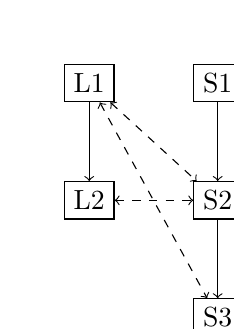
\begin{tikzpicture}
    \node[draw] (L1) {L1};
    \node[draw, below = of L1] (L2) {L2};
    \node[draw, right = of L1] (S1) {S1};
    \node[draw, below = of S1] (S2) {S2};
    \node[draw, below = of S2] (S3) {S3};
    \draw[->] (L1) -- (L2);
    \draw[->] (S1) -- (S2);
    \draw[->] (S2) -- (S3);
    \draw[<->, dashed] (L1) -- (S2);
    \draw[<->, dashed] (L1) -- (S3);
    \draw[<->, dashed] (L2) -- (S2);
  \end{tikzpicture}

  This is supposed to indicate that the read-side {\StateMachine} has
  two operations, L1 and L2, and the store machine has three, S1
  through S3, and that L1 could alias with S1 or S3 while L2 can only
  alias with S2.  This graph cannot be correctly handled if only
  directly-racing accesses are considered for permutation.  The
  algorithm will start in the configuration (L1, S1, $\varnothing$,
  false, false), and determine that L1 can race with S1 so introduce
  an $\happensBefore$ test to distinguish the two cases.  Consider the
  case where L1 is issued before S1 first.  The algorithm will now
  have to encode a {\StateMachine} for the configuration (L2, S1,
  $\varnothing$, true, false).  L2 does not directly conflict with S1,
  so it might issue L2 and S1 in either order.  If it issues L2 first
  then the read-side {\StateMachine} will complete before the
  write-side one starts, and so the {\StateMachine} will be replaced
  with just \state{Unreached}.  The result is that all orderings where
  L1 comes before S1 will be ignored.

  Now consider the case where S1 is issued before L1.  The next
  configuration to be considered is then (L1, S2, $\varnothing$,
  false, true), and L1 does not directly interfere with S2, so the
  algorithm can immediately issue S2 and move on to (L1, S3,
  $\varnothing$, false, true).  Now the only option is to issue L1, as
  otherwise the store machine will complete before the load machine
  starts, moving to (L2, S3, $\varnothing$, false, true).  Finally, L2
  does not directly interfere with S3, and so only one ordering of the
  two accesses need be considered; assume the algorithm picks L2
  first.  Now the only access considered by the cross-product
  {\StateMachine} is S1, S2, L1, L2, S3, which clearly does not
  adequately cover the potential interleavings of these two
  {\StateMachines}.
\item
  Of course, it is not always entirely clear when two accesses might
  overlap, as the addresses accessed can be completely arbitrary
  expressions.  In that case, one of the orderings will include an
  assertion that the two addresses match up and the other will not.
  This avoids needing to consider both orderings of two memory
  accesses which do not alias with each other.

  \todo{Alternative explanation: if they don't match, it doesn't
    matter which order you pick, so just pick one of them and then
    constrain the other ordering to never consider the case where they
    don't match.}
\end{itemize}

These rules, between them, implement a form of partial order
reduction\needCite{}, ensuring that the symbolic execution engine
never has to consider two executions which differ only in the ordering
of commutative operations.  This provides a useful reduction in the
state space which must be considered.

\subsection{Path explosion}

One common problem in symbolic execution systems is path explosion:
the number of paths through a program rises exponentially in the size
of the program, and this can prevent na\"ive symbolic execution
systems from being applied to realistically large programs.  In the
case of \technique, there are two main causes of path explosion:

\begin{itemize}
\item
  Aliasing.  If the various simplification passes and the dynamic
  analysis cannot determine how memory accessing instructions alias
  then the symbolic execution engine must consider every possible
  aliasing pattern, of which there are $O(n^m)$, where $n$ is number
  of \state{Load} operations and $m$ the number of \state{Store} ones.
  This grows rather quickly in the number of unsolvable aliasing
  problems, especially when the number of \state{Store}s in the
  {\StateMachine} rises.  This represents one of the major limitations
  to \technique's scalability.
\item
  Thread interleaving.  The cross-product {\StateMachine} will have
  $O(nm)$ states, where $n$ is number of states in the read-side
  {\StateMachine} and $m$ the number in the write-side one.  The
  number of paths through the combined {\StateMachine} then grows as
  $O(2^(nm))$, which again grows rather quickly.
\end{itemize}

The result is that, in the common case where the read-side
{\StateMachine} consists mostly of \state{Load} operations and
write-side one mostly of \state{Store} ones, the symbolic execution
engine might have to consider up to $O((2n)^m)$ distinct paths when
evaluating the cross-product {\StateMachine}.  This is obviously
completely infeasible for even moderate values of $n$ and $m$.  For
good performance, {\technique} is completely reliant on the various
simplification and analysis techniques to reduce $n$ and $m$ to
something manageable.  Fortunately, as discussed in the evaluation,
they are able to do so in a useful set of cases.

\subsection{Use of the induction rule}

When analysing a potential crash at instruction $i$, it is sometimes
possible to show that the existence of a bug at $i$ would imply the
existence of a bug at an earlier instruction $i'$.  This allows
{\technique} to use a form of induction to eliminate some potential
bad pointer dereference-type bugs, or at the very lest to reduce the
number of very similar bugs reported.  The idea here is to take the
read-side {\StateMachine} from a candidate bug and truncate it,
cutting it off at some memory-accessing state, in such a way that the
truncated {\StateMachine} will report a crash if the original
{\StateMachine} would have dereferenced a bad pointer at that memory
access.  A new verification condition is then generated using that
truncated {\StateMachine} as the read-side {\StateMachine} and the
original write-side {\StateMachine} as the write-side.  A bug only
needs to be reported for the original pair of {\StateMachines} if
there is some initial state which satisfies the original verification
condition but does not satisfy the truncated one.

Of course, like most forms of induction, this requires a base case in
order to be sound.  The main bug-finding analysis therefore records
every time it had to use the induction rule to eliminate a bug,
including which instruction the eliminated bug was at and which
instruction was assumed to be bug-free in order to eliminate it.  Once
the main analysis is complete this log is checked for cycles.  If it
is cycle free then the induction rule is sound.  I have not, so far,
found any programs for which the graph contains a cycle, but if a
cycle were to be found then it could sensibly be handled by selecting
a single bug from the cycle and reporting that, ignoring all others.

This rule relies on the monotonicity property of the definition of
crashes, as discussed in \S~\ref{sect:monotonicity}.  As such, it is
not sound in the presence of mandatory concurrency, and might lead to
bugs which do not require mandatory concurrency being neglected simply
because they happen to be ``near to'' a bug which does.  As argued
previously, mandatory concurrency should be rare in most programs, and
so I do not expect this to be a problem in practice.  \todo{Might want
  a bit more there?}

\todo{Forward ref eval to say how useful this is.}

\subsubsection{Mandatory concurrency}
\label{sect:mandatory_concurrency}

\todo{Making a bit of a meal of this.  Easiest answer might be to just
  drop it completely; it doesn't really add enough to justify its
  size.  Certainly doesn't belong here.}

The set of bugs detected by SLI depends on the size of the two
analysis windows.  Setting this to too small a value will of course
lead to bugs being missed; more subtly, increasing the size of the
window can also sometimes lead to the set of bugs which is reported
shrinking.  Most of the lost bugs will be false positives eliminated
by providing the analysis with more context, but there may also be a
small number of real bugs lost.  This happens when the program depends
on a certain minimum level of concurrency in order to achieve
correctness: {\technique} assumes that the program does not crash if
all of the instructions in the analysis window are run atomically, and
if the program requires some minimum level of interleaving this
assumption can be violated for some interesting executions.  Enlarging
the analysis window will make the problem worse.

\begin{figure}
\begin{tabular}{ll}
Read thread:         & Write thread: \\
\\
Load $t$ from loc1   & Load $t'''$ from loc1 \\
Store $t$ to loc2    & Store $t'''$ to loc2 \\
Load $t'$ from loc1  & Store $t''' + 1$ to loc2 \\
Load $t''$ from loc2 & \\
Crash if $t' == t''$ & \\
\end{tabular}
\label{fig:mandatory_concurrency1}
\caption{Example of threads with mandatory concurrency.}
\end{figure}

\begin{figure}
\begin{tabular}{ll}
Read thread:          & Write thread: \\
\\
Load $t'$ from loc1   & Load $t'''$ from loc1 \\
Load $t''$ from loc2  & Store $t'''$ to loc2 \\
Crash if $t' == t''$  & Store $t''' + 1$ to loc2
\end{tabular}
\label{fig:mandatory_concurrency2}
\caption{Truncation of the example in figure~\ref{fig:mandatory_concurrency1}.}
\end{figure}

As a concrete example, consider the threads shown in
figure~\ref{fig:mandatory_concurrency1}.  Running the read thread
atomically is guaranteed to crash, from any starting state, and so
there will be no valid bug tuples based on the complete definition of
these threads.  On the other hand, if the read thread is truncated as
shown in figure~\ref{fig:mandatory_concurrency2} then there may be
such a tuple:

\begin{itemize}
\item
  The R atomic rule is satisfied provided that the initial value of
  loc1 is not equal to loc2.
\item
  The W atomic rule is satisfied by any initial state.
\item
  The concurrent rule is satisfied by this crashing interleaving:
  \begin{itemize}
  \item Load $t'$ from loc1
  \item Load $t'''$ from loc1
  \item Store $t'''$ to loc2
  \item Load $t''$ from loc2
  \item Crash if $t' == t''$
  \end{itemize}
\end{itemize}

In this particular case, the crashing execution is far more likely
than the non-crashing one even when the threads are being run in
parallel and so it is highly unlikely that this precise behaviour
would be found in a real program.  On the other hand, if there were a
large amount of code between the final two load operations in the
final thread then it might make the surviving interleaving unlikely.
This is not generally an issue for SLI, as introducing enough extra
instructions to ensure that behaviour would generally push the first
load out of the analysis window so that SLI never sees the confusing
behaviour.  This means that, for most practical purposes, the set of
bugs found by increases monotonically with the size of the analysis
window, which in turn means that a very simple heuristic suffices for
setting the size of the window: use the largest window which allows
the analysis to complete in an acceptable amount of time.

\todo{It'd be nice to have some evidence of that.}

A more powerful analysis framework might be able to increase the
window size sufficiently that the first part of the read thread would
not ``fall out''.  Even in that case, the monotonicity property would
probably still hold for most realistic programs.  The fundamental
problem here is one of mandatory concurrency: in the larger program,
running the read thread in isolation is guaranteed to crash, but it
can be ``rescued'' by being interleaved with the write thread.  The
bug here is caused by insufficient concurrency, but SLI is only
capable of handling bugs caused by excessive concurrency.
Excess-concurrency bugs are far more common than
insufficient-concurrency bugs, for several reasons:

\begin{itemize}
\item
  An insufficient-concurrency bug indicates that the programmer got
  the sequential case wrong but the concurrent case correct.  The
  concurrent case is usually far more difficult to design and reason
  about than the sequential one, and so this is an unusual
  outcome\needCite{}.
\item
  The sequential case generally receives more testing than the
  concurrent one, simply as an artifact of the way most test cases are
  constructed\needCite{}.
\item
  For most programs, there are far more concurrent executions than
  sequential ones, and so it is more likely that there are errors on
  an untested concurrent path than that there are errors on an
  untested sequential one.
\end{itemize}

SLI therefore completely ignores these insufficient-concurrency bugs.

I now show that insufficient-concurrency bugs are the only case in
which the monotonicity property might be violated.  To see this,
consider execution shown in figure~\ref{fig:mandatory_concurrency3}.
Suppose that this execution does not generate a bug tuple.  Then
moving an instruction from $R$ or $W$ into $P$ also cannot generate a
bug tuple, and so by induction no smaller analysis windows can
generate bug tuples.

From the fact that larger windows do not generate bug tuples, we know
that:

\begin{itemize}
\item $P \concatDynTraces R \not= \survive$, from the R atomic rule, or
\item $P \concatDynTraces W \concatDynTraces R \not= \survive$, from the W atomic rule, or
\item $\crash \notin P \concatDynTraces (R \interleaveDynTraces W)$, from the concurrent rule.
\end{itemize}

Define $W = w \concatDynTraces W'$ and $R = r \concatDynTraces R'$, so
that $w$ is the first instruction of $W$ and $W'$ all the others, and
likewise for $r$, $R$, and $R'$.  Shrinking the analysis window then
corresponds to replacing $R$ with $R'$ and $P$ with $P
\concatDynTraces r$, or replacing $W$ with $W'$ and $P$ with $P
\concatDynTraces w$.  We therefore generate a bug tuple with the
reduced window if:

\begin{align*}
( & (P \concatDynTraces w \concatDynTraces R & = & \survive) & \wedge \\
  & (P \concatDynTraces W \concatDynTraces R & = & \survive) & \wedge \\
  & ((P \concatDynTraces w \concatDynTraces (R \interleaveDynTraces W')) & \ni & \crash)) & \vee \\
( & (P \concatDynTraces R & = & \survive) & \wedge \\
  & (P \concatDynTraces r \concatDynTraces W \concatDynTraces R' & = & \survive) & \wedge \\
  & ((P \concatDynTraces r \concatDynTraces (R' \interleaveDynTraces W)) & \ni & \crash))
\end{align*}

Combining those together, we find that reducing the analysis window can introduce a new bug if:

\begin{align*}
( & (P \concatDynTraces R & \not= & \survive) & \wedge \\
  & (P \concatDynTraces W \concatDynTraces R & \not= & \survive) & \wedge \\
  & ((P \concatDynTraces (R \interleaveDynTraces W)) & \not{}\ni & \crash)) & \vee \\
( & (P \concatDynTraces w \concatDynTraces R & = & \survive) & \wedge \\
  & (P \concatDynTraces W \concatDynTraces R & = & \survive) & \wedge \\
  & ((P \concatDynTraces w \concatDynTraces (R \interleaveDynTraces W')) & \ni & \crash)) & \vee \\
( & (P \concatDynTraces R & = & \survive) & \wedge \\
  & (P \concatDynTraces r \concatDynTraces W \concatDynTraces R' & = & \survive) & \wedge \\
  & ((P \concatDynTraces r \concatDynTraces (R' \interleaveDynTraces W)) & \ni & \crash))
\end{align*}

Simple boolean algebra, plus the obvious rule that $P \concatDynTraces (R \interleaveDynTraces W) = (P \concatDynTraces r \concatDynTraces (R' \interleaveDynTraces W) ) \cup (P \concatDynTraces w \concatDynTraces (R \interleaveDynTraces W') ) $, reduces that to this:

\begin{align*}
( & (P \concatDynTraces r \concatDynTraces R' & = & \crash) & \wedge \\
  & (P \concatDynTraces w \concatDynTraces r \concatDynTraces R' & = & \survive) & \wedge \\
  & (P \concatDynTraces w \concatDynTraces W' \concatDynTraces r \concatDynTraces R' & = & \survive) & \wedge \\
  & ((P \concatDynTraces w \concatDynTraces (W' \interleaveDynTraces R)) & \ni & \crash)) & \vee \\
( & (P \concatDynTraces r \concatDynTraces R' & = & \survive) & \wedge \\
  & (P \concatDynTraces w \concatDynTraces W' \concatDynTraces r \concatDynTraces R' & = & \crash) & \wedge \\
  & (P \concatDynTraces w \concatDynTraces r \concatDynTraces R' & = & \survive) & \wedge \\
  & (P \concatDynTraces r \concatDynTraces w \concatDynTraces W' \concatDynTraces R' & = & \survive) & \wedge \\
  & ((P \concatDynTraces r \concatDynTraces (W \interleaveDynTraces R')) & \ni & \crash))
\end{align*}

Consider the first clause of the disjunction first, and in particular consider these two terms:

\begin{align*}
 & (P \concatDynTraces r \concatDynTraces R' & = & \crash) & \wedge \\
 & (P \concatDynTraces w \concatDynTraces r \concatDynTraces R' & = & \survive)
\end{align*}

The definition of crash used in SLI is that the final instruction of $R'$ crashes, and so adding further instructions after that point cannot possible change the result.
Those terms are therefore equivalent to these:

\begin{align*}
 & (P \concatDynTraces r \concatDynTraces R' \concatDynTraces w \concatDynTraces W' & = & \crash) & \wedge \\
 & (P \concatDynTraces w \concatDynTraces r \concatDynTraces R' \concatDynTraces W' & = & \survive)
\end{align*}

In other words, $R$ is doomed when run in isolation, but running it in parallel with $W$ can save it.
That is precisely the definition of mandatory concurrency used above.

Consider the second clause now.
That contains these two terms:

\begin{align*}
  & (P \concatDynTraces w \concatDynTraces W' \concatDynTraces r \concatDynTraces R' & = & \crash) & \wedge \\
  & (P \concatDynTraces r \concatDynTraces w \concatDynTraces W' \concatDynTraces R' & = & \survive)
\end{align*}

This is even more clear: running $W$ and then $R$ atomically leads to a crash, but allowing $W$ to interrupt $R$ saves the execution.
Once again, this clause is only satisfiable in the presence of mandatory concurrency.

Therefore, it is only possible for shrinking the analysis window to reveal more bugs in the presence of mandatory concurrency, and, conversely, when the program does not use mandatory concurrency, enlarging the analysis window cannot disguise bugs.
This monotonicity property is useful because it provides a simple rule for setting the size of the analysis window: use the largest such that the analysis completes in a reasonable amount of time.
There is no need for the user to carefully select a window size for their program, or to try multiple window sizes in order to reveal additional bugs.




\section{The satisfiability checker}
This doesn't really belong here.  I should figure out where to put it.
I should also figure out whether I'd be better off using someone
else's checker.  The current one is pretty damn stupid; it tries a
couple of normal forms and then if they don't do anything useful does
an implicit analytic tableaux-type thing.

\section{Reproducing bugs}
\label{sect:reproducing_bugs}

\todo{Having written this up, I'm not convinced the idea of message
  payloads is all that useful for describing how cross-thread
  constraints are evaluated.  Nevermind.}

\todo{Should make it explicit that the CFGs we're working with here
  are the unrolled CFGs used when building {\StateMachines}, rather
  than the program's raw CFGs.}

Given a pair of {\StateMachines} and a verification condition it is
possible to build a ``crash enforcer'': a patch to the program which
will insert delays into the program's execution in a way which will
make the bug more likely to reproduce.  This can then be used to
determine which of the many bugs reported by the prior analysis are
actually reproducible, and hence to appropriately target efforts in
fixing them.  In effect, the {\StateMachine} pair is turned into a
custom dynamic analysis which targets just the bug of interest.

As an example, consider these two threads:

\begin{verbatim}
int *global_ptr[];
void thread1(int idx1) {
    if (global_ptr[idx1])
        *global_ptr[idx1] = 7;
} 
void thread2(int idx2) {
    global_ptr[idx2] = NULL;
}
\end{verbatim}

Suppose further that they compile to this machine code:

\begin{verbatim}
thread1:

l1:   ADD global_ptr + idx1 -> reg1
l2:   LOAD *reg1 -> reg2
l3:   CMP 0, reg2
l4:   jmp_if_eq l7
l5:   LOAD *reg1 -> reg3
l6:   STORE 7 -> *reg3
l7:

thread2:

l8:   ADD global_ptr + idx2 -> reg4
l9:   STORE 0 -> *reg4
\end{verbatim}

(This is essentially the bug indexed\_toctou discussed in
section~\ref{sect:eval:indexed_toctou}).  There is a risk here that
\verb|thread1| might crash if \verb|l9| is interleaved between
\verb|l2| and \verb|l5| and \verb|idx1 == idx2|.  The previous
analysis phase will detect this bug and produce the verification
condition $idx1 == idx2 \wedge l2 \happensBefore l9 \wedge l9
\happensBefore l5$.  This can then be used to augment the
control flow graph of the program with happens-before edges, as
shown in figure~\ref{fig:using:example_hb_graph}.

\begin{figure}
  \begin{tikzpicture}
    \node[CfgInstr] (l1) {l1: ADD global\_ptr + idx1 $\rightarrow$ reg1};
    \node[CfgInstr, below=of l1] (l2) {l2: LOAD ${\ast}reg1 \rightarrow reg2$};
    \node[CfgInstr, below=of l2] (l3) {l3: CMP $0, reg2$};
    \node[CfgInstr, below=of l3] (l4) {l4: JMP\_IF\_EQ };
    \node[CfgInstr, below=of l4] (l5) {l5: LOAD ${\ast}reg1 \rightarrow reg3$ };
    \node[CfgInstr, below=of l5] (l6) {l6: STORE $7 \rightarrow {\ast}reg3$ };
    \node[CfgInstr, below=of l6] (l7) {};
    \node[CfgInstr, right=of l1] (l8) {l8: ADD $global\_ptr + idx2 \rightarrow reg4$};
    \node[CfgInstr, below=30mm of l8] (l9) {l9: STORE $0 \rightarrow {\ast}reg4$};
    \draw[->] (l1) -- (l2);
    \draw[->] (l2) -- (l3);
    \draw[->] (l3) -- (l4);
    \draw[->,ifFalse] (l4) -- (l5);
    \draw[->,ifTrue] (l4.west) to [bend right=70] (l7);
    \draw[->] (l5) -- (l6);
    \draw[->] (l6) -- (l7);
    \draw[->] (l8) -- (l9);
    \draw[->,happensBeforeEdge] (l2) -- (l9);
    \draw[->,happensBeforeEdge] (l9) -- (l5);
  \end{tikzpicture}
  \caption{CFG with happens-before edges for the example.}
  \label{fig:using:example_hb_graph}
\end{figure}

The task is then to modify the program so as to make it more likely
that this happen-before graph will be satisfied when the program runs
while leaving its behaviour otherwise unchanged.  This can be
accomplished by inserting small delays into the program's execution.
In this case, simply inserting a delay before \verb|l5| would probably
be sufficient, as that would enlarge the critical section and hence
make it more likely that the critical store will intervene.

\begin{figure}
  \begin{tikzpicture}
    \node[draw] (A) {A};
    \node[draw, above right = of A] (X) {X};
    \node[draw, below right = of X] (B) {B};
    \node[draw, above right = of B] (Y) {Y};
    \node[draw, below right = of Y] (C) {C};
    \draw[->] (A) -- (B);
    \draw[->] (B) -- (C);
    \draw[->] (X) -- (Y);
    \draw[->,happensBeforeEdge] (A) -- (X);
    \draw[->,happensBeforeEdge] (X) -- (B);
    \draw[->,happensBeforeEdge] (B) -- (Y);
    \draw[->,happensBeforeEdge] (Y) -- (C);
  \end{tikzpicture}
  \caption{A happens-before graph which cannot be reproduced by
    inserting a single delay.}
  \label{fig:enforce_crash:complex_hb}
\end{figure}

More complex happens-before graphs can make it more complex to
determine where delays should be inserted.  Consider, for instance,
the happens-before graph shown in
figure~\ref{fig:enforce_crash:complex_hb}.  This is intended to show
two threads, one which executes instructions A, B and C in order and
the other which executes X and then Y, where the behaviour of interest
only happens with the interleaving A, X, B, Y, C.  There is no simple
critical section structure here, making it less obvious where delays
need to be inserted.  Even once it has been determined where to insert
the delays, deciding their magnitude remains non-trivial: the delay
between X and Y for instance, must be large enough to be confident
that B happens before Y if A happens before X, but not so large that C
is also likely to happen before Y.  Simply picking the largest delay
which avoids unacceptable performance overheads risks masking such
bugs.  Solving such constraints requires a far more detailed model of
the program's structure and the time taken by various instructions,
and such models are both difficult to derive and fragile once they are
available.

{\Technique} avoids this problem by using a message-passing system.
The core idea is to model a happens-before ordering X before Y as a
message which is sent by X, after it completes, and collected by Y,
before it starts.  These messages are synchronous: the sender will
wait for the receiver, and the receiver will wait for the sender, in
both cases with a short timeout.  In the first example, there will be
two messages, one sent from \verb|l2| to \verb|l9| and the other sent
from \verb|l9| to \verb|l5|, with delays be inserted immediately
before \verb|l9| and \verb|l5|, and also immediately after \verb|l2|
and \verb|l9|.  These delays have slightly different functions:

\begin{itemize}
\item
  The delay after \verb|l2| makes the read-side of the critical
  section wait for a matching write-side.  In effect, this delay
  enlarges the read-side critical section in the hope that a
  write-side operation will come along which can be dropped into it.
  This is useful for bugs where the write-side occurs much more
  frequently than the read-side.
\item
  The delay before \verb|l9| makes the write-side wait for a matching
  read-side.  The intuition here is that the enforcer will maintain a
  ``pool'' or write-side operations which can then be deployed as soon
  as a read-side operation turns up.  This is useful for bugs where
  the read-side occurs much more frequently than the write-side.
\item
  The delays after \verb|l9| and before \verb|l5| help the read- and
  write-sides of the critical section to proceed with the desired
  interleaving.  By this point, the two threads have rendezvoused and
  been bound together, and so there is no need to wait for a matching
  operation to arrive.  The delay is instead used to wait for the
  paired thread to reach the appropriate place in its control-flow
  graph (or to exit the simulation, causing the message operation to
  fail).  The timeout is in this case necessary only to prevent
  deadlocks: it is possible that the program contains some
  synchronisation structure of which SLI is unaware, so that one
  thread might be waiting for the other, and introducing an additional
  unbounded wait would be unsafe.

  \todo{The difference between bound and unbound message operations is
    important; it deserves more discussion than this.  There's a lot
    later on, but it should be brought up here.}
\end{itemize}

Setting the sizes of these delays, especially those after \verb|l2|
and \verb|l9|, involves a delicate trade-off between performance and
the likelihood of uncovering bugs.  In general, SLI will choose one of
\verb|l2| or \verb|l9| as a delay-able instruction, according to their
relative frequency, and use a large timeout for the delay-able
instruction and a very small one for the non-delay-able one.  This is
discussed further in section \ref{sect:using:timeout_balancing}.

Encoding the second example as a message-passing system requires more
message operations but does not introduce any additional conceptual
complexity: messages are sent from A to X, X to B, B to Y, and Y to C,
with potentially large delays at the message operations at A and X to
allow threads to rendezvous and smaller ones at the other instructions
to keep them synchronised once they have.

This basic message passing scheme is sufficient to ensure that the
instructions of the program obey the happens-before graph, assuming
that the initial rendezvous succeeds.  That is sufficient to trigger
the desired behaviour in some cases but not all; in particular, it can
be insufficient if there is some additional non-trivial side-condition
required before the bug reproduces.  Suppose, for instance, that the
read- and write-side {\StateMachines} are operations on some dynamic
structure and that there are many instances of the structure in the
running program.  The bug will only be reproduced if the two threads
happen to access the same instance of the structure.  Because there
are many such instances is likely to be a low-probability event and
the probability of the bug being reproduced remains very low even when
all happens-before relationships are satisfied.  Even worse, the
additional delays mean that the buggy code is likely to run less often
than it otherwise would, and so enforcing the happens-before graph in
isolation might actually make the bug less likely to reproduce per
unit time.

Fortunately, {\technique} already knows about all such
side-conditions, as they form the bulk of the verification condition
whose derivation has already been discussed.  This problem can then be
avoided if the crash enforcer checks the verification condition at the
same time as it enforces the happens-before graph.  Once a
verification condition has failed there is no need to insert
additional delays, reducing the overhead of the enforcement patch and
increasing the likelihood of the desired bug being exhibited.

In the case of the example, the verification condition is $idx1 ==
idx2$, and so we are only interested in executions where the two
indices coincide.  There is then one immediate complication: $idx1$ is
a local variable in one thread, and $idx2$ is a local variable in a
different thread.  There are no points in the original program which
know the values of both variables, and so no obvious place in which to
check the condition.  {\Technique} solves this problem by checking the
condition as part of the \verb|l2| to \verb|l9| message operation.  If
\verb|l2| is delayed while sending the message, it will publish the
value of \verb|idx1| to a globally-accessible location, and \verb|l9|
will then check that as part of its receive operation.  If the indices
do not match, the receive operation fails and \verb|l9| will continue
waiting for another sender (subject to an appropriate timeout).
Likewise, if \verb|l9| is delayed while receiving the message it will
publish the value of \verb|idx2|, and this will then be checked by any
other thread trying to send the message from \verb|l2|.  A timeout
balancing mechanism then adjusts the timeouts so that both \verb|l9|
and \verb|l2| occur with reasonable frequency and so a message
operation is likely to succeed eventually, provided that the bug
really is possible.

The result of this phase is a crash enforcement plan specifying when
messages need to be sent, what side conditions need to be checked, and
also which registers or other per-thread state need to be stored for
later use.  The original program can then be modified so as to follow
this plan when possible.  I present two basic mechanisms for doing so:
an interpreter, which must interpret the original program's machine
code while it is executing instructions involved in the plan, and a
compiler, which avoids the interpreter by compiling the plan down to
machine code, hence improving performance but at the expense of less
effective handling of some corner cases.  As a further refinement, I
also present a scheme for combining multiple enforcers, so that
several bugs can be investigated at once.

\todo{The implementation of the compiler is currently broken.  Need to
  decide whether I'm going to fix it or just drop that bit.}

\subsection{Outline of algorithm}

At a high level, the algorithm used has the following phases:

\begin{itemize}
\item
  Heuristically simplify the crash summary.  The main bug-finding
  analysis phase attempts to be sound, within parameters already
  discussed, which can sometimes lead to the verification condition
  containing clauses which might in theory influence the behaviour of
  the program but in practice are highly unlikely to.  The first phase
  of building a crash enforcement plan is to remove some of these
  clauses.  This is discussed in
  section~\ref{sect:enforce:heuristic_simplify}.
\item
  ``Slice'' the verification condition according to the possible
  happens-before graphs. As discussed in
  section~\ref{sect:intro:overview}, {\technique} can correctly
  capture the happens-before graph necessary for a bug to reproduce
  even when that happens-before graph is data-dependent.
  Unfortunately, those data-dependencies make it difficult to encode
  the happens-before graph into a simple message passing system.
  {\Technique} therefore re-expresses the verification condition as a
  function of the happens-before graph, effectively eliminating the
  dependency.  This is discussed in more detail in
  section~\ref{sect:enforce:slice_hb_graph}.
\item
  The algorithm now considers each possible happens-before graph in
  turn and, for each one:

  \begin{itemize}
  \item
    Determines what information is needed to evaluate the verification
    condition, in terms of the machine registers and the contents of
    memory, and where that information first becomes available;
  \item
    Decides where to evaluate the various clauses of the verification
    condition;
  \item
    Defines the ``payload'' data which must be included in the various
    messages.
  \end{itemize}

  This is discussed in section~\ref{sect:enforce:place_vcs}.
\item
  If appropriate, multiple enforcers can be combined at this point,
  which can sometimes make it easier to discover bugs if the initial
  analyses have produced a very large pool of candidates.  More
  details are given in section~\ref{sect:enforce:combine_enforcers}.
\item
  Decide on a strategy for gaining control of the program at
  appropriate points.  The crash enforcement plan only imposes
  constraints on instructions which are likely to be involved in the
  target bug, which is usually a tiny fragment of the entire program.
  It would be deeply unfortunate if the entire program had to be
  rewritten to insert the necessary modifications; quite aside from
  the greater risk of bugs, the performance would probably be quite
  poor.  The interpreter is obviously far slower than running machine
  code directly, and even the compiler introduces non-trivial
  overheads.  As such, it is necessary to modify the original program
  so that {\technique} can gain control when the program reaches one
  of the interesting fragments of code.
  Section~\ref{label:sect:assign_entry_points} discusses how this is
  done.

\item
  Depending on the desired mode of operation, the plan is then passed
  to either the plan interpreter, discussed in
  section~\ref{sect:enforce:interpreting}, or the compiler, discussed
  in section~\ref{sect:enforce:compiling}.  In either case, the result
  is an ELF shared object which can be loaded into the target program
  to enforce the plan \todo{(at least for {\implementation})}.
\end{itemize}

\subsection{Heuristic simplifications of the {\StateMachines} }
\label{sect:enforce:heuristic_simplify}

\todo{There's some intuition here that the important thing is
  maintaining satisfiability of the verification condition.  Not
  really sure how to make that explicit.}

The crash summaries generated by the main analysis often contain a lot
of redundant information, and this can complicate the process of
enforcing the crash.  The first phase of generating an enforce is
therefore to remove this ancillary information.  Most obviously, all
of the parts of the {\StateMachines} used only to provide hints to the
simplifiers and symbolic execution engine can be dropped:
\state{Assert}, \state{PointsTo}, \state{StartFunction}, and so forth.
This often allows further simplifications by, for instance, making
some of the variables used in the assertions dead, or by making states
which differ only in their calling context more easily unified.

This phase also uses some heuristics to simplify the verification
condition, such as assuming that $x {\times} k = y {\times} k
\Leftrightarrow x = y$ for all constants $k$.  This is not necessarily
true for ordinary integer arithmetic due to integer overflow issues,
but is in practice true often enough to be a sensible assumption.

Next, the R atomic and W atomic parts of the verification condition
can be removed.  These restrict the analysis to only consider the case
where running some combination of the {\StateMachines} atomically
would survive.  This is appropriate when trying to determine
statically whether a concurrency bug might exist, but is unlikely to
be helpful when trying to enforce a concurrency bug.  If R atomic
fails then the read-side is likely to crash without any help from a
concurrent thread, and so the pattern of delays which the enforcer
applies is unlikely to make a great deal of difference either way.
Having the enforcer attempt to check R atomic is therefore rather
pointless.  Likewise, seeing the W atomic constraint fail usually
indicates that the program has a bug, but it is not one which the
enforcer can do anything about.  The analysis therefore re-derives R
atomic and W atomic constraints and simplifies the verification
condition under the assumption that both are true.

Note that this is not quite the same as simply replacing the
verification condition with the crash possible constraint, as the
information in the atomic constraints will have been used to constrain
the paths considered during symbolic execution of the cross-product
{\StateMachine}.  \todo{Should really figure out whether that's
  actually a good thing or not.}

\todo{This suggests another possible validation thing for the eval: do
  something which evaluates R atomic and W atomic instead of trying to
  enforce the HB graph and see how often they fail.  R atomic,
  certainly, should never fail.  W atomic might due to synchronisation
  things, so that might turn out to be less interesting.}

\subsubsection{Removal of redundant clauses}

\todo{Really not convinced that this is actually a good idea in
  practice.  The original justification was making the bugs easier for
  a person to understand, and it sometimes helps here, but it equally
  easily make things worse.  Maybe just kill it.}

These simplifications can sometimes mean that the verification
condition includes constraints on program-level values which are no
longer mentioned anywhere in either of the {\StateMachines}.  These
clauses tend not to provide very much useful information, and so it
makes sense to remove them.  At the same time, it is important not to
remove apparently-redundant variables which mediate between
interesting ones.  For instance, if the verification condition were
$thread1:RBX = thread2:RCX \wedge thread2:RCX = thread2:RDX \wedge
thread2:RCX = 7$, where $thread1:RBX$ and $thread2:RDX$ appear in the
{\StateMachines} but $thread2:RCX$ does not, it would not be
appropriate to remove the references to $thread2:RCX$.  On the other
hand, if the condition were $thread1:RBX = thread2:RDX \wedge
thread2:RCX = 7$ then it would be useful to remove the constraint on
$thread2:RCX$ and produce a verification condition of just
$thread1:RBX = thread2:RDX$.  \todo{Not sure how much I believe that,
  now that I've written it down, but nevermind.  Also, that's a really
  stupid example; come up with a better one.}

At a high level, the idea here is to factor the verification condition
into a conjunction of independent clauses and then eliminate any
clauses which do not constrain the behaviour of the {\StateMachines}.
{\Technique} does this in a very simple way: convert the verification
condition to conjunctive normal form, build an interference graph
whose vertices are variables and which has an edge between variables
whenever those vertices appear together in a clause, and then find all
of the connected components of this graph.  These components are the
independent clauses of the factorisation.  Any which do not mention
any variables which are also mentioned by the {\StateMachines} can be
safely discard. \todo{Ref Gaifman graphs?}

This is not a particularly efficient algorithm, due to the need to
convert to conjunctive normal form, and often takes an intractable
amount of time for complicated verification conditions.  Fortunately,
it is also optional: even when this simplification fails, the
resulting enforcer is still \todo{in some sense} correct, although it
may often be slower or less effective than it otherwise would be.  If
failure of this phase were a problem then it could probably be
improved using, for instance, the techniques discussed in \todo{find
  something to cite.  There must be something; this is a pretty damn
  common problem if you're doing theorem proving, and this cannot be
  the best way of solving it.}

One important subtlety here is the definition of variable.  Some, such
as program registers, are obvious, but others, such as initial-memory
$LD$ expressions are more subtle.  The problem is that $LD(addr)$
expressions depend on the address loaded and it is not always apparent
whether two $LD$ expressions might possibly alias, and hence whether
they should be treated as the same variable.  {\Technique} solves this
problem by segregating the $LD$ expressions into groups which might
alias and treating each such group as a value, so that $LD(addr)$ is
considered to influence $LD(addr')$ if there is any possibility that
$addr$ might equal $addr'$.  This is conservative but safe.

\todo{Maybe mention that testing $addr = addr'$ depends on where
  abouts in the {\StateMachine} the load is mentioned?  Or is that too
  obvious?}

\todo{Also mention that $BadPtr$ expressions get the same sort of
  treatment.}

\todo{HB edges: the input {\StateMachines} don't usually contain any
  HB edge, but we assume that an edge $a \happensBefore b$ is
  mentioned if either $a$ or $b$ are mentioned anywhere.}

\subsubsection{Removal of underspecified clauses}

\todo{This is easier to justify as a preliminary to satisfiability
  checking, rather than a simplification prior to building the
  enforcer, but it is rather useful here.}

In a similar vein, if a variable is never mentioned in the
{\StateMachines} and is mentioned precisely once in the verification
condition then its value is unlikely to be particularly enlightening.
The intuition here is again that a constraint is most likely to be
important when it influences the satisfiability of the verification
condition, and such a single-use variable will very rarely do so.
Alternatively, the single use of the variable can be regarded as its
definition, in which case there is a definition of a variable which is
never used and so the definition can be removed.  These variables are
referred to as underspecified, because the verification condition and
{\StateMachines} do not meaningfully constraint their values.  This
generalises easily to expressions by saying that an expression is
underspecified if the presence of underspecified variables means that
it can be set to anything at all.  The verification condition is, at
this stage, usually a conjunction of clauses, and any clauses which
are underspecified can simply be discarded.

\todo{Not sure that's all that clear.}

\subsection{Slicing the verification condition by happens-before graph}
\label{sect:enforce:slice_hb_graph}

\todo{This is often rather expensive, and is always rather stupid.
  Need to come up with a better way of doing it.  Obvious way is to
  re-express the VS as a BBDD and then just reorder all the
  $\happensBefore$ variables to the root of the DAG, at which point it
  all becomes trivial.}

{\STateMachines} and verification conditions are capable of
representing data and control flow dependent happens-before graphs,
but the message passing mechanism used in the crash enforcement phase
is not capable of enforcing such things.  It is now therefore
necessary to remove these dependencies.  The approach taken by
{\implementation} is to just re-express the verification condition as
a function of the happens-before graph, deriving a new verification
condition for each possible graph.  These new conditions can then be
treated independently and recombined as if they were enforcers for
completely independent bugs, as discussed in
section~\ref{sect:enforce:combine_enforcers}.

This re-expression is itself straightforward: enumerate all of the
$\happensBefore$ expressions in the verification condition and then
consider all combinations of those expressions in turn, generating a
new verification condition for each.  This could potentially generate
$2^n$ new verification conditions, and hence might appear to be
computationally unpleasant.  In practice, it is usually tolerable, for
two main reasons:

\begin{itemize}
\item
  Most bugs do not involve a particularly large number of
  happens-before edges, and so $n$ is usually small (\todo{Cite
    preemption bounding and CHESS papers}, for instance, obtained good
  results while limiting the number of happens-before edges to at most
  2).
\item
  Most bugs do not have a data-dependent happens-before pattern, and
  so usually all but one of the potentially verification conditions
  can be eliminated very quickly.  Those which do have data-dependent
  happens-before requirements will usually only have a very small
  number of interesting graphs (although it is possible to design
  artificial bugs which require an arbitrarily large number).
\end{itemize}

Even better, most of the time, behaviours which require a large number
of happens-before edges will be quite restricted in when they
reproduce, and so avoiding one easy case is negatively correlated with
avoiding the other.

\todo{Somewhat surprisingly, this is quite a long way from being the
  most expensive part of the analysis.  Should really try to get some
  numbers on what the expensive part actually is.}

Treating the different graphs as completely independent does not,
therefore, lead to an excessive increase in the cost of generating the
enforcer.  It does, however, lead to some inefficiency in the enforcer
itself, as it is not possible to shared common expressions between the
different bugs.  When combining completely unrelated enforcers this is
not usually a problem, as there are unlikely to be many common
expressions anyway, but this is not true when combining closely
related enforcers.  A more elegant approach would be to allow
enforcers to share a common prefix and then only have them diverge
once they encounter the data-dependent happens-before components.  I
have not implemented such an optimisation.

\subsection{Placing the evaluation of verification conditions}
\label{sect:enforce:place_vcs}
The verification condition has now been factored into a happens-before
graph such that if the happens-before graph is enforced while the
side-condition holds then the bug is highly likely to reproduce.  The
next step is to determine how the side-condition is to be evaluated,
in terms of where program registers are to be sampled, what
side-conditions need to be checked at each instruction, and what
information needs to be included with the happens-before messages.

\todo{Hmm.  For various implementation reasons which I don't really
  want to go into, the VC is highly likely to be a conjunction of
  mostly-independent clauses at this point, and I kind of rely on that
  in the placing strategy.  I should really come up with a better way
  of doing that, or at least a sane justification for assuming that
  the VC is a conjunction.}

The main correctness constraint on the placement of these expressions
is that they cannot be evaluated before all of the necessary inputs
are available.  These inputs consist of the initial values of
processor registers for the various threads and the control-flow
variables indicating how the threads progress through their CFG
fragments\footnote{Note that $LD$ initial memory expressions are
  \emph{not} considered as inputs to side-condition validation, as the
  side-condition checker can itself fetch the necessary data from
  program memory as soon as the address of the $LD$ is evaluatable.}.
The initial value of a processor register is considered to be
available throughout the relevant thread and control-flow variables
are available in the relevant thread as soon as the relevant part of
the control-flow graph is reached.  In addition, any messages sent
between threads make any values available in one thread available in
the other.  Side-conditions can then be evaluated as soon as all of
their inputs are available.

Once the side conditions have been placed in the control-flow graph
the next step is to decide which registers and control-flow variables
need to be samples, and where in the graph that should be done.  In
the case of control-flow variables there is only one possible place to
capture them: when the relevant control-flow edge is traversed.
Initial register values, on the other hand, allow slightly more
flexibility.  In principle, they should be captured at the first
instruction in the control-flow graph; they are the initial value of
the register in the CFG, after all.  This can, however, sometimes lead
to the program spending longer than necessary in the interpreter, and
hence poor performance if the side condition usually fails.  This is
because most instructions do not modify most registers.  If the only
reason to trap to the interpreter is to capture the \verb|RDI|
register then no trap is necessary until the program reaches an
instruction which might modify \verb|RDI|.  {\Implementation}
therefore optimises the crash enforcement plan slightly by deferring
register sampling operations, if necessary deferring side-condition
checking at the same time, if doing so is safe and would allow the
interpreter to start later.

\subsection{Enforcing the plan}

Previous sections described how to build a crash enforcement plan,
consisting of a set of CFG fragments annotated with the crash
enforcement operations:

\begin{itemize}
\item Program registers and control-flow variables to be sampled.
\item Side-conditions to be checked.
\item Messages to be sent and received.
\end{itemize}

Our task now is to force the program to follow this plan.
{\Implementation} implements two mechanisms for doing so:

\begin{itemize}
\item
  An interpreter with well-defined semantics, a high likelihood of
  successfully imposing the plan, and some useful theoretical
  properties, but very high run-time overheads.  This is described in
  section~\ref{sect:enforce:interpreting}.
\item
  A compiler which makes far more approximations, and hence is far
  less likely to impose the plan successfully and far less
  analytically tractable, but which has slightly lower run-time
  overhead.  This is described in section~\ref{sect:enforce:compiling}.
\end{itemize}

\label{sect:enforce:assign_entry_points}
Regardless of whether the plan is to be interpreted or compiled, the
next step is to arrange to gain control of the program at appropriate
points, meaning any instruction which might be the start of one of the
CFG fragments.  For clarity of exposition, I here assume that the plan
is to be interpreted rather than compiled; the algorithm used for
compiled enforcers is essentially identical. {\Implementation} does so
by modifying the original program to contain branches into either the
plan interpreter where necessary.  This has very low runtime overhead
and avoids excessively permuting the program's state, but has one
critical disadvantage: the instruction at which {\implementation}
needs to gain control might be smaller than a branch instruction, and
so inserting the branch might cause additional instructions in the
program binary to be corrupted.  {\Implementation} must then ensure
that the program never attempts to execute one of these corrupted
instructions.  For performance reasons, we would also like to minimise
the number of instructions which must be run in the interpreter.

This is most easily understood as a kind of search problem.  The
algorithm starts in a state in which the original program is not
modified at all, but with a list of instructions at which it must gain
control; it must then find a path to a state in which it is guaranteed
to gain control at all necessary points and the program is guaranteed
never to branch to a corrupted instruction.  More explicitly, these
states consist of three sets:

\begin{itemize}
\item $Patch$ --- instructions at which we have decided to place a
  branch instruction.
\item $Cont$ --- instructions which might not themselves be patched,
  but which must be processed in the interpreter.  The program will
  not branch to the interpreter when it encounters one of these
  instructions, but if the interpreter has already started when one
  needs to be run then the interpreter will continue, even if that
  means leaving the CFG fragments described in the main plan.
\item $MustInterpret$ --- instructions where the plan requires us to
  gain control, but where the patches described in this state would be
  insufficient to do so.
\end{itemize}

The search process then generates additional states according to two
rules:

\begin{itemize}
\item
  \textbf{PatchDirect} An instruction is removed from $MustInterpret$
  and added to $Patch$.  The analysis then examines the instructions
  which would be corrupted by that new entry point to determine
  whether there are any potential branches to them and, if so, adds
  those branches to $MustInterpret$.  The corrupted instructions are
  themselves added to $Cont$.

  This rule is only valid when the existing $Patch$ set does not
  itself contain any patch operations which would overlap with the new
  patch point, as these branch instructions would otherwise corrupt
  each other and lead to an unrealisable solution.
\item
  \textbf{Prefix} As with \textbf{PatchDirect}, an instruction is
  removed from $MustInterpret$, but in this case it is added to $Cont$
  and any instruction which might branch to it added to
  $MustInterpret$.  The idea here is that if we can ensure that all
  instructions which execute immediately prior to an instruction $i$
  are executed in the interpreter and if the interpreter continues
  interpreting when it sees a branch to $i$ then that is sufficient
  to ensure that $i$ is also run in the interpreter.
\end{itemize}

Any state with an empty $MustInterpret$ set then represents a valid
solution to the patching problem.  The number of instructions in
$Cont$ is a rough proxy for the number of additional instructions
which will have to be interpreted due to the corrupted instructions
problem, and hence for the overheads of the patching process, and so
the search process aims to minimise the $Cont$ set.  Usefully, both
rules increase the size of $Cont$ and so a simple exploration strategy
which always selects the state in the queue with the smallest $Cont$
set, applies both rules to that state, and places the two new states
in the queue is guaranteed to always find the minimal result, and this
is the strategy adopted by {\implementation}.

One complication here is that the algorithm needs to be able to find
the predecessors of an instruction.  In the fully general case this is
an impossible thing to determine for an arbitrary binary.
{\Technique} makes two key assumptions in order to solve it:

\begin{itemize}
\item
  Functions are only ever entered at their entry point, as determined
  by the analysis described in section~\ref{sect:function_head}.  In
  particular, any branches from dynamically generated or library code
  back into the main program must branch to a function head.
\item
  For any dynamic branch within a function, the dynamic analysis
  observes all possible targets of that branch.
\end{itemize}

Given those assumptions, the static analyses already discussed can
determine all of the branches to any instruction in the program except
for a function head, and can detect whether an instruction is a
function head.  {\Technique} then simply disables any rule which
requires it to calculate the predecessors of a function head.

This can sometimes lead to the patch problem being unsolvable if the
entire function is smaller than a single branch instruction, as in
that case it is possible that neither rule might be enabled at the
function head.  In that case, {\implementation} simply gives up and
reports an error.  This is rarely a problem in practice, as very few
functions are that small without very aggressive compiler
optimisations, and most compilers, including gcc and LLVM\needCite{},
will at high optimisation levels pad functions to a multiple of 16
bytes for performance reasons.

The assumption that the dynamic analysis is complete is more of a
problem.  This can sometimes lead to the program executing one of the
corrupted instructions if its behaviour deviates significantly from
that observed during dynamic analysis.  That is just about tolerable
in a tool such as {\technique}'s crash enforcers, which are only
intended as a debugging aid for knowledgeable programmers, but is more
of a concern when {\technique} is being used to fix bugs. \todo{I'm
  going to need to say something clever here.}

This problem was also tackled by the AutoPaG project, and the solution
they developed is similar. \todo{Similar but not the same.  They use a
  dominator-based scheme, and hence avoid needing the global branch
  information but can end up with much larger patches and a higher
  risk of deadlocks/starvation problems.  The original version of SLI
  used basically the same algorithm (although I did it first); should
  probably explain why I had to switch.}

An alternative approach would be to take control of the program using
debug breakpoints rather than jump instructions.  These are either a
single byte (for the \verb|int3| instruction) or no bytes at all (for
debug registers), and so avoid the instruction clobbering problem.
This would work, but would have a couple of important disadvantages:

\begin{itemize}
\item
  Debug breakpoints are far slower than branches.  This might be
  important if the critical section is to be inserted on a
  particularly hot code path and has a side-condition which usually
  fails.
\item
  Using debug breakpoints in this way would interfere with any other
  debugger which the developer might want to use.  With a branch-style
  patch, standard debuggers work without modification for any part of
  the program which has not been patched, whereas a breakpoint-style
  patch requires extensive coordination between the debugger and the
  patch mechanism for either to work at all.
\item
  Breakpoint registers are of strictly limited number on most
  architectures (four, on x86).  This means that they can never
  provide a complete solution by themselves.
\item
  On most UNIX-type operating systems, including Linux and FreeBSD,
  catching debug breakpoints requires modifying the program's signal
  handling configuration, which requires some level of coordination
  with the program to be modified.  It would be possible to use an
  alternative API, but this would require kernel modifications,
  complicating the use of the generated patches.
\end{itemize}

SLI therefore generates exclusively branch-style patches.

\todo{I did implement a breakpoint-based scheme, so it might be
  interesting to actually include some numbers on their relative
  effectiveness.}

\todo{Placing patch points is actually the most computationally
  expensive step of building the enforcer, once you've got the VC.  I
  might need to do some implementation work to make that a bit less
  crazy.}

Of course, a patch strategy which ensures that the interpreter gains
control at appropriate instructions is not quite the same as one which
ensures that the interpreter gains control at appropriate CFG nodes,
because {\technique} CFG nodes are identified by stack context in
addition to their raw instruction pointer.  The interpreter must
therefore be able to check this call stack.  The mechanisms used in
the interpreter and the compiler are slightly different and here I
only describe the one used in the interpreter; the compiler variant is
deferred to the rest of the compiler discussion.

\todo{Already given this algorithm once, in the stack normalisation
  section!}

\label{sect:using:find_return_address}
The interpreter has access to all of the process registers and the
stack when it gains control.  The challenge here is to locate the
return addresses on the stack, without access to either debug symbols
or a frame pointer, so that the function calling context can be
properly checked.  SLI uses a static analysis, performed when
generating the crash enforcement plan, to solve this problem.  The
static analyses already described are sufficient to determine the
entry point of the function containing a given RIP, and so it is easy
to perform a simple abstract interpretation forwards from that point
to the given RIP and hence find the number of bytes which the function
will push onto the stack on the way\footnote{This is generally fixed
  for all possible paths, due to the way in which most compilers are
  implemented.}.  The first entry in the call stack is trivially true
because of the way the jumps are patched in.  The second one is the
return address of the current function, which can be found using that
offset.  The third one is the return address of the calling function,
and the offset there is just the previous offset plus the offset in
the calling function.  In this way all necessary offsets can be found
and the entry-point stack checked completely.


\subsection{Interpreting the plan}
\label{sect:enforce:interpreting}

\todo{This feels like it needs some cites in here somewhere.  Not sure
  what I should be citing, though.}

The plan interpreter runs in the address space of the target program
and, as already discussed, arranges to take control of the program at
the plan entry points.  It then interprets the program's machine code,
enforcing the plan as it goes, until the plan either completes or
fails\footnote{The machine code interpreter used is a lightly modified
  version of the one used by the Xen hypervisor\needCite{}.}.  In
either case, the interpreter then restores the target program's
register state and branches back to the original program's code.  If
the plan completed successfully the program should then quickly crash,
having suffered the bug which is to be reproduced.  Otherwise, the
program continues unmolested in the hope that there will be another
opportunity to reproduce the bug later on.

\todo{Need to talk somewhere about what happens if you try to enforce
  contradictory HB graphs at the same time.  The results really aren't
  very pretty.}

The enforcement plan can be thought of as a program in a very simple
language.  Unfortunately, the semantics of this language are
non-deterministic, in the sense that the interpreter must often choose
between several possible options using information which only becomes
available later in the execution.  {\Technique} resolves this issue
using a power set-like construction\editorial{Probably want a cite for
  that, maybe.} which allows it to explore both branches of the
non-determinism simultaneously, up to some level of approximation.
The easiest way to describe this is to first define a low-level,
abstract, semantics for the interpreter, using a look-ahead
nondeterministic choice operator, and then implement a higher-level,
concrete, interpreter which effectively interprets sets of lower-level
interpreters in lockstep parallelism.  The higher-level interpreter
resolves the non-deterministic choice by forking the lower-level
interpreter as necessary, allowing all of the low-level interpreters
to execute at first and later discarding any which fail.  I present
the abstract semantics for the low-level interpreter first and then
move on to discuss the subtleties involved in implementing the
higher-level interpreter afterwards.

The non-deterministic language emulates the annotated CFG one node at
a time.  For each node, it proceeds through several stages:

\begin{itemize}
\item[Sample] Sample processor registers and store them in the
  low-level state structure, as demanded by the plan.  This might
  allow some side-conditions to be evaluated and, if so, they are
  evaluated here.  If any fail then the low-level interpreter
  exits; otherwise, it proceeds to state RX.
\item[RX] Receive any message demanded by the plan, evaluating any
  post-receive side-conditions as we do so.  If any side-conditions
  fail then the plan fails and the low-level interpreter exits.  The
  details of receiving a message are moderately subtle, even in the
  abstract semantics, and are discussed in more detail below.
\item[Emul] Emulate the original program's instruction corresponding
  to this CFG node.  This includes issuing any necessary memory
  accesses, updating processor registers, and branching, as
  appropriate.
\item[TX] Send any message demanded by the plan.  This is, again,
  somewhat subtle, and is discussed later.
\item[Succ] Find successor instructions.  The emulation phase will
  have determined the instruction pointer of the next instruction to
  be executed, and this must now be mapped into a CFG node so that
  execution can continue.  There are four main cases:

  \begin{itemize}
  \item
    The CFG node has no successors at all.  The plan has completed
    successfully and the interpreter exits; if everything has worked,
    the program will soon crash having suffered the bug which is being
    investigated
  \item
    The CFG node has successors but none match up with the desired
    next instruction pointer.  In that case, the interpreter can
    proceed no further.  The plan fails and the interpreter exits.
  \item
    Precisely one of the successor nodes has the desired instruction
    pointer.  The interpreter simply advances to that node.
  \item
    Multiple successor nodes have the desired instruction pointer.
    The most common reason for this is loop unrolling: if a loop in
    the program is unrolled three times, say, then the CFG node for
    the instruction just prior to the loop will have four successors,
    corresponding to skipping the loop completely or running it once,
    twice, or three times.  It is not possible, at this stage, to
    determine how many times the loop must be run, and so the abstract
    interpreter makes a non-deterministic choice between all of the
    available options.
  \end{itemize}

  If the plan requires any control-flow variables to be sampled then
  this is done here.  This might in turn allow additional
  side-conditions to be evaluated; if so, these side-conditions are
  used to restrict the set of possible successor states in the obvious
  way.
\end{itemize}

\subsubsection{Sending and receiving messages in the abstract semantics}

The message send and receive operations are moderately involved.  If
both the sending and receiving interpreters are known then the
operation can be modelled by this simple Petri net:

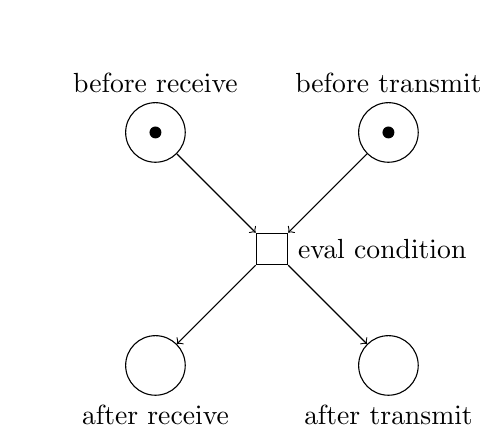
\begin{tikzpicture}
  \node[place,tokens=1,label=above:{before receive}] (beforeRx) {};
  \node[transition,below right=of beforeRx, label=right:{eval condition}] (trans) {};
  \node[place,tokens=1,above right = of trans, label=above:{before transmit}] (beforeTx) {};
  \node[place,tokens=0,below left = of trans, label=below:{after receive}] (afterRx) {};
  \node[place,tokens=0,below right = of trans, label=below:{after transmit}] (afterTx) {};
  \draw[->] (beforeRx) -- (trans);
  \draw[->] (beforeTx) -- (trans);
  \draw[->] (trans) -- (afterRx);
  \draw[->] (trans) -- (afterTx);
\end{tikzpicture}

The message can only be discharged if the side condition holds, and
the side condition can only be evaluated once both threads reach the
message operation.  While the message is being processed the two
interpreters are effectively joined together and can be treated as if
they were executing in the same thread, and so the side condition can
reference the private state of both interpreters.  Once the condition
has been evaluated the two interpreters separate and the threads can
execute independently until the next message operation.

In a real implementation, of course, the threads are not
pre-specified, and most of the complexity of the message algorithm
lies in determining them.  The basic idea here is that a message send
or receive operation should rendezvous with any receive or send which
occurs near enough in the program execution.  This is illustrated in
figure~\ref{fig:enforce:message_windows}: each message operation
defines a window in the program's execution, and the interpreter must
arrange to synchronise with any message operation whose interval
overlaps with the current message's.  In the abstract semantics, which
allows lookahead non-deterministic choice, this is implemented by
non-deterministically choosing whether or not to wait and then failing
if that turned out to be the wrong choice.  The receive algorithm is
therefore like this:

\begin{figure}
  \begin{minipage}{80mm}
    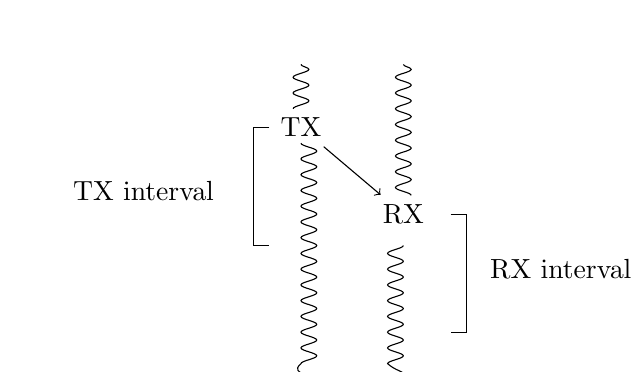
\begin{tikzpicture}
      \draw[->,decorate,decoration={snake,segment length=2mm, amplitude=1mm}]
        (0mm,0mm) -- (0,-5mm)
        (0mm,-8mm) node (TX) {TX} (0,-10mm) --
        (0mm,-40mm);
      \draw (-4mm,-8mm) -- (-6mm,-8mm) -- (-6mm,-23mm) -- (-4mm,-23mm);
      \draw (-20mm,-16mm) node {TX interval};

      \draw[->,decorate,decoration={snake,segment length=2mm, amplitude=1mm}]
        (13mm,0mm) -- (13mm,-16mm)
        (13mm,-19mm) node (RX) {RX} (13mm,-23mm) --
        (13mm,-40mm);
      \draw (19mm,-19mm) -- (21mm,-19mm) -- (21mm,-34mm) -- (19mm,-34mm);
      \draw (33mm,-26mm) node {RX interval};
      \draw[->] (TX) -- (RX);
    \end{tikzpicture}
    Intervals overlap; message is sent.
  \end{minipage}
  \begin{minipage}{35mm}
    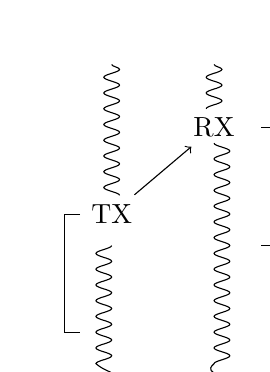
\begin{tikzpicture}
      \draw[->,decorate,decoration={snake,segment length=2mm, amplitude=1mm}]
        (0mm,0mm) -- (0,-16mm)
        (0mm,-19mm) node (TX) {TX} (0,-23mm) --
        (0mm,-40mm);
      \draw (-4mm,-19mm) -- (-6mm,-19mm) -- (-6mm,-34mm) -- (-4mm,-34mm);

      \draw[->,decorate,decoration={snake,segment length=2mm, amplitude=1mm}]
        (13mm,0mm) -- (13mm,-5mm)
        (13mm,-8mm) node (RX) {RX} (13mm,-10mm) --
        (13mm,-40mm);
      \draw (19mm,-8mm) -- (21mm,-8mm) -- (21mm,-23mm) -- (19mm,-23mm);
      \draw[->] (TX) -- (RX);
    \end{tikzpicture}
    Intervals overlap; message is sent.
  \end{minipage}
  \begin{minipage}{35mm}
    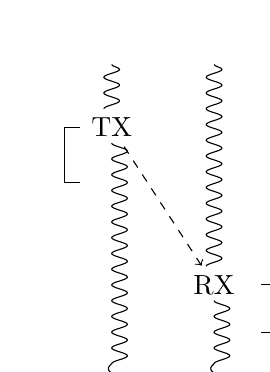
\begin{tikzpicture}
      \draw[->,decorate,decoration={snake,segment length=2mm, amplitude=1mm}]
        (0mm,0mm) -- (0,-5mm)
        (0mm,-8mm) node (TX) {TX} (0,-10mm) --
        (0mm,-40mm);
      \draw (-4mm,-8mm) -- (-6mm,-8mm) -- (-6mm,-15mm) -- (-4mm,-15mm);

      \draw[->,decorate,decoration={snake,segment length=2mm, amplitude=1mm}]
        (13mm,0mm) -- (13mm,-25mm)
        (13mm,-28mm) node (RX) {RX} (13mm,-30mm) --
        (13mm,-40mm);
      \draw (19mm,-28mm) -- (21mm,-28mm) -- (21mm,-34mm) -- (19mm,-34mm);

      \draw[->,dashed] (TX) -- (RX);
    \end{tikzpicture}\\
    Intervals do not overlap; no message can be sent.
  \end{minipage}
  \caption{Overlapping TX and RX intervals allow the message to be
    sent, regardless of which operation is ordered first.  If the
    intervals do not overlap then no message can be sent.}
  \label{fig:enforce:message_windows}
\end{figure}

\begin{algorithmic}[1]
  \If {The low-level interpreter has a bound interpreter}
    \If {The bound interpreter is not attempting to send a message}
      \State {Wait until it does so}
    \EndIf
    \State {Set $s'$ to the bound interpreter's outgoing message}
  \Else
    \State {Collect all outstanding unbound send operations as the set $s$}
    \State {Choose $s'$ non-deterministically from $s + \bot$}
    \If {$s' = \bot$}
      \State {Register the interpreter as a receiver of unbound messages}
      \State {Wait for the RX interval}
      \State {Unregister the interpreter as a receiver of unbound messages}
      \State {Collect all outstanding unbound send operations as the set $s$}
      \State {Select $s'$ non-deterministically from $s$}
    \EndIf
  \EndIf
  \If {$s'$ passes the side condition}
    \State {Discharge the message, unblocking the bound interpreter and moving to the Emul state}
  \Else
    \State {The plan has failed and the interpreter exits}
  \EndIf
\end{algorithmic}

The send operation is symmetric:

\begin{algorithmic}[1]
  \If {The low-level interpreter has a bound interpreter}
    \If {The bound thread is not attempting to receive a message}
      \State {Wait for it to do so}
    \EndIf
    \State {Set $s'$ to the bound interpreter's message receive operation}
  \Else
    \State {Collect all outstanding unbound receive operations as the set $s$}
    \State {Choose $s'$ non-deterministically from $s + \bot$}
    \If {$s' = \bot$}
      \State {Register the interpreter as a sender of unbound messages}
      \State {Wait for the TX interval}
      \State {Unregister the interpreter as a sender of unbound messages}
      \State {Collect all outstanding unbound receive operations as the set $s$}
      \State {Select $s'$ non-deterministically from $s$}
    \EndIf
  \EndIf
  \If {$s'$ passes the side condition}
    \State {Discharge the message, unblocking the bound interpreter and moving to the Succ state}
  \Else
    \State {The plan has failed and the interpreter exits}
  \EndIf
\end{algorithmic}

The behaviour when $s' = \bot$ is perhaps somewhat surprising: the
thread waits a little while and then selects a peer thread to
discharge the message with non-deterministically.  Meanwhile, all of
the other threads are simultaneously performing similar
non-deterministic choices.  The use of look-ahead nondeterminism means
that all of the threads will make these selections in a mutually
compatible way, so that there is no danger of A attempting to
discharge its message with B while B discharges with C.  The actual
implementation must resolve these constraints much more carefully, and
is discussed in detail later.

\subsubsection{Timeout balancing}
\label{sect:using:timeout_balancing}

Selecting the size of the various timeouts is important for
determining the likelihood of reproducing a bug and the overheads of
enforcing the patch.  SLI does so primarily dynamically, in response
to the program's observed behaviour.  I now consider briefly how these
timeouts should be set.

By far the most important timeouts are those which occur when unbound
interpreters synchronise, as bound-interpreter delays only happen when
the bug is already quite likely to reproduce, so assume for now that
those are the only two delays.  There are two such delays, one for
sending the first message and one for receiving it.  Call them $D_1$
and $D_2$.  Assume that the two CFGs occur randomly with rates $R_1$
and $R_2$.  Now the overhead introduced by the delays is $D_1.R_1 +
D_2.R_2$.  Ignoring side conditions, the bug will be reproduced if the
two CFGs occur such that the intervals on their initial message
operations overlap; in other words, if they occur with time $D_1 +
D_2$ of each other.  To put it another way, each occurrence of CFG 2
defines a window in the execution of size $D_1 + D_2$ such that the
bug will reproduce if CFG 1 starts anywhere in that window.  CFG 1
starts randomly with rate $R_1$, and so the probability of any give
instance of CFG 2 reproducing the bug is roughly $R_1(D_1 + D_2)$,
provided CFG 1 is sufficiently rare that we can neglect the
probability of two instances occurring in the window.  The expected
rate of bug reproduction is therefore $R_1.R_2.(D_1+D_2)$.  Some
simple algebra then allows us to show that if the desired overhead is
$k$, the reproduction rate will be

\begin{displaymath}
\alpha = k.R_2 + R_2.D_2(R_1 - R_2)
\end{displaymath}

So that if $R_1 > R_2$ the reproduction rate for a given level of
overhead is maximised by setting $D_2$ as large as possible, and
conversely if $R_2 > R_1$ the rate is maximised by setting $D_2$ as
small as possible.  In other words, if the total delay is fixed, it
should always all be apportioned to one side of the message operation.
{\Implementation} therefore keeps a counter of how many times the send
and receive sides of each message operation are attempted; if the send
operation has been attempted more times than the receive one then the
send operation delay is set to zero, and otherwise the receive delay
is set to zero.

\todo{Implementation currently sets the non-zero delay to some
  arbitrary constant plus a random fuzz; the next paragraph is an
  ambition.}

It now remains to set whichever of $D_1$ and $D_2$ is not fixed at
zero.  Assume without loss of that this is $D_2 = 0$.
{\Implementation} then selects $D_1$ so as to achieve a particular
level of overhead $k$ by setting $D_1 = \frac{k -
  \frac{D_0}{R_2}}{R_1}$, where $D_0$ is an estimate of the cost of
entering the interpreter and then immediately exiting.  This is not,
in fact, a constant, due to the need to sometimes interpret additional
instructions as determined by the patch strategy or to check
side-conditions before considering a message operation, but
{\implementation} uses the constant time 100$\mu$s anyway.

\subsubsection{Implementing non-deterministic choice in the Succ phase}

It might be that an instruction has several possible successors in the
control flow graph in the crash execution plan, and in that case the
interpreter must choose one of these successors using look-ahead
non-determinism.  This cannot be implemented in any
physically-realisable system, as it is non-causal, and so SLI must
emulate it.  SLI uses a power-set construction to do so.  Rather than
operating a single interpreter context, the actual implementation
maintains a set of low-level interpreter contexts, which individually
follow the abstract semantics given above, and interprets them all in
lock-step parallelism.  When one of these low-level interpreters needs
to perform a non-deterministic choice between $n$ possible values, the
high-level interpreter creates $n$ successor low-level interpreter
states, one corresponding to each possible outcome of the choice, and
inserts all of them into its current-state set.  They are then
interpreted in parallel until enough information is available to
resolve the earlier choice, at which point all but one of the threads
will exit and the interpreter can revert to ``single-threaded''
execution mode.  If a thread is bound when it performs a
non-deterministic choice then its bound thread must also be
duplicated, to ensure that the new thread has something to bind to.

One subtlety here is that the original program's underlying
instruction can only be retired once, and so the high-level
interpreter must ensure that all low-level interpreters arrive at that
point in the execution cycle at the same time.  SLI actually enforces
a slightly stronger constraint, which is that every low-level
interpreter in a given high-level interpreter must be at the same
phase in the instruction execution cycle.  The semantics given above
is designed to ensure that this always possible.  The only phases for
which it is difficult are the message send and receive phases, which
are discussed in more detail in the next section.

\subsubsection{Concrete implementations of message send and receive}

The abstract semantics given above for message send and receive
operations is not realisable on any physical hardware as it relies on
non-causal nondeterministic lookahead.  Moreover, the power-set
construction used to resolve the non-deterministic Succ state is not
sufficient here as the message operation involves a sleep operation,
and hence has non-revocable externally visible side effects.  Solving
this problem requires the message operation to be ``turned inside
out'', restructuring it into a fragment which occurs before the sleep
and another fragment which occurs after it with the remaining
non-determinism confined to the two fragments.  The resulting message
receive operation looks like this:

\todo{Urk; big wall of algorithm.  This cannot be the best way of
  describing this.}

\begin{algorithmic}[1]
  \State {$lls \gets $ the set of currently-active low-level interpreter states}
  \State {$newLls \gets $ an empty set of low-level interpreter states}
  \For {$l$ in $lls$}
    \If {$l$ does not receive any messages}
      \State {Move $l$ from $lls$ to $newLls$ without changing it}
    \ElsIf {$l$ has a bound thread}
      \If {$l$'s bound thread has exited}
        \State {$l$ exits as well; remove it from $lls$ without adding it to $newLls$}
      \ElsIf {$l$'s bound interpreter's sending-bound-message flag is set}
        \If {The bound interpreter's outgoing message passes any side condition}
          \State {Move $l$ from $lls$ to $newLls$}
          \State {Clear the bound interpreter's sending-bound-message flag}
        \Else
          \State {$l$ exits; remove it from $lls$}
        \EndIf
      \Else
        \State {Set $l$'s receiving-bound-message flag}
      \EndIf
    \Else \Comment{Unbound receive}
      \For {$s$ registered unbound senders}
        \If {$s$'s outgoing message passes the side condition}
          \State {$l' \gets $ duplicate $l$}
          \State {$s' \gets $ duplicate $s$}
          \State {Bind $l'$ and $s'$ together}
          \State {Insert $l'$ into $newLls$}
          \State {Insert $s'$ into $s$'s high-level interpreter's active low-level interpreter list}
        \EndIf
      \EndFor
      \State {Register $l$ as an unbound receiver}
      \State {Set the minimum delay to the receive operation's delay, if it is currently less than that.}
    \EndIf
  \EndFor

  \If {$lls$ is empty}
    \State \Return
  \EndIf

  \State {$end \gets now() + bound\_delay$}
  \If {There is a minimum delay}
    \State {Sleep for the minimum delay}
  \EndIf

  \While {There are bound receives in $lls$ and $now() < end$}
    \State {Wait for some bound receive to complete, or for the current time to pass $end$}
    \For {$l$ performing bound receives in $lls$}
      \If {$l$'s bound thread has exited}
        \State {Remove $l$ from $lls$}
        \State {$l$ exits}
      \ElsIf {$l$'s receiving-bound-message flag is clear}
        \State {Remove $l$ from $lls$}
        \State {Add $l$ to $newLls$}
      \Else
        \State Continue waiting
      \EndIf
    \EndFor
  \EndWhile

  \For {$l$ in $lls$}
    \If {$l$ is registered as an unbound receiver}
      \State {Unregister $l$ as an unbound receiver}
    \EndIf
    \If {$l$'s receiving-bound-message flag is set}
      \State {Exit $l$} \Comment{Receiving bound message failed}
    \ElsIf {$l$ is unbound}
      \State {$l$ must have been attempting an unbound receive which failed, so it exits}
    \Else
      \State {Add $l$ to $newLls$}\Comment {Receive succeeded}
    \EndIf
  \EndFor
\end{algorithmic}

For clarity, I have omitted the synchronisation on the various
interpreter-internal structures.  The send algorithm is symmetrical,
simply replacing the word ``receive'' with the word ``send'' and vice
versa.  There are a couple of features to note in this algorithm:

\begin{itemize}
\item
  If there are any unbound message operations then it waits for the
  whole of that message's delay, even if some other interpreter which
  might match the operation arrives.  This reflects the semantics
  already discussed in which any message operation will synchronise
  will all other matching operations in its window.  On the other
  hand, it can lead to poor performance, and the slight loss of
  correctness from ending the wait early is very rarely important.
  \todo{Say more.}
\item
  When interpreters are bound together both interpreters are
  duplicated.  This means that the original interpreter is left in the
  unbound send state, and can therefore synchronise with any
  additional interpreters which might arrive.
\item
  Bound messages use a different delay strategy to unbound ones.  This
  is because bound operations fail in different ways.  By
  construction, a bound interpreter will eventually either exit or
  perform all planned message operations and so it might appear that
  bound operations should never hit their timeout, and that is indeed
  the common case.  It is, however, possible, albeit very rare, for
  {\technique} enforcers to introduce a deadlock if they interact
  badly with the program's existing synchronisation structure.  These
  timeouts avoid that issue.  \todo{Actually, now I think about it, I
    don't think that deadlock is actually possible, but I don't want
    to have to prove that, so maybe just pretend that it is.}
\end{itemize}

Note that the side condition is evaluated as the message is being
discharged, while the two interpreters are merged.  \todo{This is
  incomprehensible, which is a pity because it's also quite
  important.} It is possible to imagine an alternative implementation
in which discharging the message copies enough state from the
transmitting interpreter to the receiver to allow the condition to be
evaluated locally in the receiver after the interpreters have been
unmerged\footnote{Or, conversely, one where state is copied from the
  receiver to the transmitter and the side-condition evaluated in the
  transmitter after transmission.}.  This would reduce the size of the
synchronised section and so would appear, on the face of it, to offer
greater parallelism, and hence potentially better performance.
Unfortunately, it does not work.  To illustrate the problem, consider
again the example shown in figure~\ref{fig:using:example_hb_graph}.
One thread modifies a shared structure while another thread reads it,
and the program will crash if the two threads happen to be operating
on the same structure at the same time.  Suppose that the read thread
runs far more often than the write one and that there are many
instances of the structure.  The timeout balancing logic will quickly
reduce the delay on the read side's first message send to zero and
increase the delay on the write side's first message receive to
compensate.  Now, when the write interpreter does run it will stop
just before \verb|l9| waiting for a matching read interpreter to
arrive.  By hypothesis, many such interpreters will arrive, as the
read thread runs more often than the write one.  In the alternative
design, the side condition can only be evaluated in the receiving
interpreter once the message operation is complete.  In this case the
receiving interpreter is the write thread, and so every read
interpreter will be forced to bind to the write thread.  Only one
interpreter can be bound to the write thread at any one time, and so
satisfying these later attempts to bind will force the write
interpreter to be duplicated many times.  Because of timeout
rebalancing, the read interpreter will proceed from \verb|l2|
immediately and quickly reach \verb|l5|, where it has to receive a
message from \verb|l9|.  At this point, there are two possible
outcomes:

\begin{itemize}
\item
  The read interpreter is delayed at \verb|l5| waiting for the message
  from \verb|l9|.  The write interpreter is still waiting in case any
  other threads reach \verb|l2| and attempt to synchronise with it,
  and so this might potentially be a rather long delay.  Since the
  read thread runs far more often than the write thread, this will
  have a very large performance impact.  Worse, it will probably be
  pointless: there are, by hypothesis, a large number of instances of
  the structure which is being examined, and so, with high
  probability, the write thread will be modifying a different one.
  When the write interpreter does finally escape from its receive
  delay and evaluate the side condition it will discover that the
  filter fails, and so the write thread will exit.  The read thread
  will then discover that its bound thread has exited and be forced to
  exit as well.  The crash enforcement plan will therefore not
  complete and the bug is highly unlikely to reproduce.
\item
  The thread is not delayed at \verb|l5|.  It never receives the
  message from \verb|l9| and must therefore exit without completing
  the plan, so is unlikely to reproduce the bug.  The write thread's
  high-level interpreter will then accumulate a collection of
  low-level threads which have bound to exited read threads and which
  will themselves immediately exit.
\end{itemize}

Neither outcome helps to reproduce the target bug.

By contrast, in the scheme used by SLI, the read thread is able to
evaluate the side condition at \verb|l2| and will therefore only bind
to write threads which modify the structure which it is reading.  That
means that the thread can be delayed a relatively long time at
\verb|l5| without fear of apocalyptic performance damage, and so the
bug will reproduce relatively easily.

One further optimisation, not shown here but implemented in
{\implementation}, avoids redundantly duplicating low-level
interpreter contexts in the common case that a message operation is
discharged precisely once.

\subsubsection{Starting new low-level interpreters}

The high-level interpreter is responsible for starting new low-level
interpreters as the program under test moves through CFG nodes which
are marked as entry point nodes.  This might be because the program
has just reached one of the interpreter entry point instructions,
already discussed in the discussion of building patch strategies.  It
might also be because the program has reached an entry point while
running under the interpreter, in which case the high-level
interpreter must start another low-level interpreter to handle the new
CFG.  This can happen if the one of the CFG fragments is
cyclic\editorial{Or as cyclic as the unrolled CFG fragments ever
  get...} and re-enters itself, or if two of the CFG fragments
overlap.  {\Implementation} handles either case by spawning additional
low-level interpreters.  After starting a new low-level interpreter
the high-level interpreter must sample the value of any needed
processor registers and evaluate any appropriate side-conditions, as
already discussed.  The new low-level interpreter can then be added to
the high-level interpreter state and interpretation proceeds as
already discussed.

\subsubsection{The await-bound-thread-exit state}

When a thread completes its plan, it is sometimes useful for it to
wait for its bound thread to exit before proceeding.  This is because
the crash summary from which the plan is generated does not have
complete information on the structure of the program and can miss
relevant stores which happen after the write-side {\StateMachine}
completes.  If the last edge in a happens-before graph is from memory
access A to memory access B, that usually means that A is a store and
B is a load and B must load the value stored by A.  That means that,
not only must B happen after A, but B must happen before any other
writes to the memory location modified by A.  If there were other
stores to that location in the crash summary then the happens-before
graph would include additional edges to ensure that that happens, but
if there are stores outside of the analysis window then it will not.
For instance, suppose that the write thread looks like this:

\begin{verbatim}
while (1) {
l1:  *x = 5;
l2:  *x = 7;
     <something_complicated>
}
\end{verbatim}

And the read thread looks like this:

\begin{verbatim}
l3: a = *x;
l4: b = *x;
    crash if a != b;
\end{verbatim}

This program is clearly buggy.  One way of reproducing this bug would
be to interleave instructions as \verb|l1|, \verb|l3|, \verb|l2|,
\verb|l4|, and SLI will discover this interleaving as the
happens-before graph show in figure~\ref{fig:enforce:await_exit_hb}.
The algorithm described so far will be sufficient to enforce this
graph (assuming that the two fragments of code shown can actually
execute in parallel) but may still struggle to reproduce the bug.
This is because the generated happens-before graph is incomplete: it
misses the edge from \verb|l4| to \verb|l1| in the next iteration of
the loop.  If the loop completes and reaches the store at \verb|l1|
before the load \verb|l4| completes then the bug will not reproduce
even though the happens-before graph was successfully enforced.  The
workaround for this problem is simple: if a low-level state ends with
a successful message send then the sending thread is not allowed to
execute any further instructions until the receiving thread has either
completed a further instruction or has itself exited.  This ensures
that activity beyond the analysis horizon cannot prevent bug
reproduction, and, because it only happens when the plan is mostly
complete, and thus very rarely, it has very low performance overhead.

\begin{figure}
\begin{tikzpicture}
\node[CfgInstr] (l1) {l1};
\node[CfgInstr, below = of l1] (l2) {l2};
\node[CfgInstr, right = of l1] (l3) {l3};
\node[CfgInstr, below = of l3] (l4) {l4};
\draw[->] (l1) -- (l2);
\draw[->] (l3) -- (l4);
\draw[->,happensBeforeEdge] (l1) -- (l3);
\draw[->,happensBeforeEdge] (l3) -- (l2);
\draw[->,happensBeforeEdge] (l2) -- (l4);
\end{tikzpicture}
\caption{Happens before graph for the await-bound-exit example.}
\label{fig:enforce:await_exit_hb}
\end{figure}

\subsection{Combining multiple enforcers}
\label{sect:enforce:combine_enforcers}

The initial static analysis and symbolic execution phase can generate
a large number of false positives, and it would be extremely tedious
to have to test each one independently.  {\Implementation} therefore
includes a mechanism for enforcing multiple bugs at once.

\todo{How does this work?  Actually very simple: you generate
  mostly-independent plans for each VC, and then have the high-level
  interpreter start low-level interpreters for each of them as
  appropriate.  The only time it gets complicated is when you have
  contradictory happens-before graphs, but I don't have a good story
  for that yet.}

\subsection{Run-time considerations}

Evaluating side conditions is not always completely trivial, even once
all of the inputs are available.  In particular, $LD(addr)$
expressions require a moderate amount of care.  These are defined to
return the contents of memory at a particular address.  The problem is
that the address might turn out to be a bad pointer, and it is
important for the enforcer not to cause the program to crash in that
case.  {\Implementation} solves this problem by simply catching page
faults generated while evaluating side conditions.  If any such faults
occur then the relevant low-level interpreter state is considered to
have failed.  This is not always ideal from the point of view of
reproducing the bug, but avoids spuriously crashing the program under
test.

\todo{Another major approximation: $LD$ is supposed to return the
  initial contents of memory, but that's not necessarily available.
  The enforcers evaluate $LD$s as soon as they can evaluate the
  address to be loaded, which is pretty much as good as you can get,
  but it's still not \emph{quite} right.}

\todo{Why do we sometimes end up dereferencing pointers which the
  program never does? Answer: because the placement stuff sometimes
  ends up pulling validation over program control flow, which makes it
  easier to implement and easier to fast-out of the enforcer, but
  risks introducing these bad dereferences.}

\subsection{Compiling the plan}
\label{sect:enforce:compiling}

\todo{Implementation of this is currently massively broken; need to
  decide whether I'm going to fix it or just use a slightly older
  version, or just drop it completely.  Also, some of the
  simplifications to the semantics described here aren't really
  necessary or well thought-through.  Also, doing this is completely
  bloody pointless.}

In addition to a plan interpreter, SLI also includes a plan compiler, which combines the plan with the program's original machine code to produce a modified version of the program which performs the necessary enforcement actions without needing an interpreter.
The intent here is to reduce the overhead of the interpreter in the case where SLI is investigating many bugs most of which do not exist.
Making this practical requires several simplifications to the semantics:

\begin{itemize}
\item
  The number of physical program threads operating in the plan is limited.
  In particular, it is assumed that only one program thread will be executing the read side of the plan at any time, and likewise only one thread will be executing the write side.
\item
  The message semantics are simplified: messages are sent asynchronously, with a delay only on the read side, and must be ``cancelled'' when the relevant thread exits.
  This has two important implications: first, that a message send can never fail and, second, the something must keep track of what messages a given thread currently has outstanding.
  Combined with the first simplification, it also means that at most one instance of any given message can be outstanding at any one time, and so it is easy to place the relevant information in a global structure without needing any dynamic memory allocation.
\item
  High-level interpreter contexts only ever access the state of their own low-level interpreters.
  This has two important implications:

  \begin{itemize}
  \item
    Remote low-level interpreters are never duplicated during message operations.
    If the normal semantics would require an interpreter to be duplicated then the local message operation fails.
  \item
    The receive message filter can only be executed by the receiving thread after receiving a message.
  \end{itemize}
\item
  When a low-level interpreter is duplicated due to a non-deterministic choice in the Succ phase the low-level state's stash table is not duplicated.
  Instead, all low-level interpreters in a given high-level interpreter share a single stash table.
\end{itemize}

The result is a system with lower run-time overheads, but also a lower probability of reproducing interesting bugs.
It has a much larger I-cache footprint but a smaller D-cache one\editorial{Not sure where I'm going with that, although it is true and kind of interesting}.

I now briefly outline the implementation of this compiler.
The core idea is to compile the CFG in the enforcement plan into a state machine.
This state machine consists of a large number of smaller intra-instruction state machines, as illustrated in figure~\todo{...}, each of which models a single instruction in the original program.
The label on each state is itself a set of low-level labels which consist of a four-tuple of the plan thread which is executing, a reference to the plan CFG node, a set of messages which have been sent by the thread, and the phase of the intra-instruction state machine.
Each state is compiled to a small fragment of machine code (which might be empty, if this instruction does not have an relevant annotation in the plan) plus a set of relocations specifying the fragment's relationships to the other states.
Once every state has been compiled these relocations can be discharged and the fragments concatenated together to form the final patch.

I now discuss the details of each phase of the intra-instruction machine:

\begin{itemize}
\item[RecvMsg]
  Examine the set of CFG nodes which are active in the current state and determine whether the plan requires any of them to receive messages.
  If so, emit code to examine the global outstanding-message structures to see whether of the desired messages are currently outstanding.
  If there are, receive precisely that message.
  Any other message receive operations are considered to have failed and the relevant CFG nodes removed from the current state label.
  If no message sends are currently outstanding then the physical thread is delayed until either one is available or some timeout is reached.
  If a message becomes available then it is received, and otherwise all receives fail and all receiving CFG nodes are removed from the label.
  Note that this does not necessarily mean that the state label will become empty\footnote{Although that is the common case.} as there may be some CFG nodes which do not need to receive messages.

  Once a message is received its content is simply copied from the global message area into the local thread's stash area.
\item[OrigInstr]
  Store any generated values into simulation slots and issue the original instruction.
  There are three main cases to consider here:

  \begin{itemize}
  \item
    Simple memory loads.
    If the instruction is of the form \verb|LOAD *location -> register|, and the value loaded is to be saved, then it is sufficient to just copy \verb|register| into the simulation slot after the original instruction has completed.
  \item
    Compound memory loads.
    Instructions which load from memory but are not themselves simple loads are more difficult to handle.
    For concreteness, suppose that the instruction is \verb|CMP 76,*loc1|, and the annotation requires us to save the value loaded.
    The instruction loads from \verb|*loc1| but does not leave the result in any locations which we can easily access.
    It would be possible to solve this problem by adding another load of \verb|*loc1|, but that would run the risk of a store in a remote thread modifying \verb|*loc1| between the two loads, leading to very confusing results.
    SLI instead solves this problem by rewriting the instruction to this:

\begin{verbatim}
LOAD *loc1 -> reg1
STORE reg1 -> simslot
CMP 76, reg1
\end{verbatim}

    This exposes the loaded value to the instrumentation framework, allowing it to be stored to the simulation slot as desired.

    Instructions which modify memory in-place, such as \verb|ADD 1 + *loc1 -> *loc1|, pose a similar problem and can be solved in the same way, provided that they do not have a \verb|LOCK| prefix.
    \verb|LOCK|ed instructions are more complex, as separating the load and store phases into separate instructions would violate the semantics of the program and might introduce new bugs.
    SLI solves this problem using a \verb|CMPXCHG| loop.
    For instance, the instruction \verb|LOCK ADD 1 + *loc1 -> *loc1| would be converted to this machine code fragment:

\begin{verbatim}
1: LOAD *loc1 -> reg1
ADD 1 + reg1 -> reg2
LOCK CMPXCHG *loc1, reg1 -> reg2
if_cmpxchg_failed goto l1
STORE reg1 -> simslot
\end{verbatim}

    The \verb|CMPXCHG| instruction here is supposed to be an invented syntax for the x86 machine code instruction which atomically compares \verb|*loc1| to \verb|reg1| and, if they are equal, sets \verb|*loc1| to \verb|reg2|.
    This allows SLI to expose the value of the implicit load while preserving the \verb|LOCK| semantics of the original instruction.
  \item
    Branch instructions are deferred to the FindSucc state.
  \end{itemize}
  
\item[SendMsg]
  Send any outgoing messages.
  This amounts to simply copying the message payload into the global message area, setting a global flag to indicate that the message is currently outstanding, and adding the message ID to the state label's set of sent messages.
  This always succeeds and advances to the FindSucc state.

\item[ExitThread]
  When a low-level thread exits it is necessary to cancel any messages which it has sent.
  The compiler takes the union of all of the sent-messages sets in its low-level, removes the thread which is to exit, and then takes the union again.
  Any messages present in the first set but not the second need to be cancelled by setting the relevant global message-outstanding flag to zero.
  The compiler will then either exit the patch, if the last low-level thread has exited, or resume the intra-instruction state machine at an appropriate place.
\end{itemize}


\begin{tikzpicture}
\node[flowChartState] (RecvMsg) {RecvMsg};
\node[flowChartState,above left = of RecvMsg] (StartThread) {StartThread};
\node[flowChartState,above right = of RecvMsg] (CheckForThreadStart) {CheckForThreadStart};
\node[flowChartState, below = of RecvMsg] (OrigInstr) {OrigInstr};
\node[flowChartState, below = of OrigInstr] (VerfCond) {VerfCond};
\node[flowChartState, below = of VerfCond] (SendMsg) {SendMsg};
\node[flowChartState, below = of SendMsg] (FindSucc) {FindSucc};
\node[flowChartState, right = of VerfCond] (CondFail) {CondFail};
\node[flowChartState, right = of CondFail] (Exit) {Exit};
\node[flowChartState, left = of RecvMsg] (RecvdMsg) {RecvdMsg};
\draw[->] (CheckForThreadStart) -- (RecvMsg) -- (OrigInstr) -- (VerfCond) -- (SendMsg) -- (FindSucc);
\draw[->] (StartThread) to [bend right=10] (CheckForThreadStart);
\draw[->] (CheckForThreadStart) to [bend right=10] (StartThread);
\draw[->,dashed] (FindSucc.east) to [bend right=75] (CheckForThreadStart.east);
\draw[->] (RecvMsg) -- (RecvdMsg) -- (OrigInstr);
\draw[->] (RecvMsg) -- (Exit);
\draw[->] (VerfCond) -- (CondFail) -- (Exit);
\draw[->] (FindSucc) -- (Exit);
\end{tikzpicture}

  
\section{Fixing bugs using global locks}
\label{sect:fix_global_lock}

In addition to finding bugs, SLI can also be used to fix them in a
largely automated fashion.  The basic approach here is to binary patch
the program to introduce a new global lock covering the program's
relevant instructions, preventing them from executing in parallel and
hence preventing the bug from occurring (assuming that the relevant
instructions have been correctly identified).  The relevant
instructions are duplicated into a binary patch, unrolling loops and
tracing across function boundaries in a way which reflects the
function inlining and loop unrolling performed during the initial CFG
generation phase, and the duplicates modified to acquire and release
the lock at appropriate points.  The original program is then patched
to branch to the duplicates when necessary.

The first step in producing such a fix is correctly identifying the
instructions which must be included in the critical sections.  These
will be roughly a subset of the instructions involved in the
control-flow graphs associated with \StateMachines; a subset because
some instructions in the CFG do not need to be protected, and roughly
because some instructions not in the CFG will also be included in the
critical section.

\todo{Already explained this once in the context of building crash
  summaries and enforcers!}

As an example of the former, consider a program like this:

\begin{verbatim}
read_side() {
    ptr = complicated_local_calculation();
    dptr = *ptr;
    if (dptr != NULL) {
       dptr = *ptr;
       *dptr = 5;
    }
}
write_side() {
    ptr = complicated_local_calculation();
    *ptr = NULL;
}
\end{verbatim}

Here, the read thread computes some pointer using entirely local
operations, loads from it once and then, if the result is
non-\verb|NULL|, loads from it again and uses the resulting pointer.
Meanwhile, the store thread sets a potentially coincident memory
location to \verb|NULL|.  The read thread clearly has a potential
time-of-check, time-of-use race bug.  The {\StateMachines} generated
by {\technique} will include the buggy code itself but might also
include part or all of \verb|complicated_local_calculation()| and a
side-condition which requires the two pointers to match up.  This
extra information is useful when analysing the bug
(\S\ref{sect:using:check_realness}) or when attempting to reproduce it
(\S\ref{sect:using:reproducing_bugs}) but cannot be used by this kind
of instruction-level fix\footnote{But see future work for a possible
  alternative scheme which would make use of it.}, so including it in
the fix is unhelpful and would tend to lead to unnecessarily large
critical sections.  The fix generating process must therefore select a
useful subset of the instructions in the control-flow graph.

The approach taken here is simple:

\begin{itemize}
\item
  Extract all of the happens-before edges from the bug summary's
  verification condition.  These entirely capture the
  instruction-interleaving parts of the bug to be fixed, and, since
  instruction-interleaving is the only thing which can be influenced
  by this type of patch, the resulting set of edges contains all of
  the useful information in the condition.
\item
  Identify all of the CFG nodes which are mentioned in one of those
  happens-before edges.
\item
  Trim the CFG such that every path starts and ends in one of those
  mentioned nodes.  All such paths will be included in a critical
  section, and so no such paths will be permitted to execute in
  parallel.
\end{itemize}

In this way the CFG is restricted to just those instructions which are
involved in the interleaving which is to be prevented.

Note that this is not guaranteed to produce an optimal selection of
critical sections, in the sense that sections can sometimes be larger
than is strictly necessary.  Consider, for example, a program with the
same read side as the previous example but a write side in which the
pointer is assigned to twice:

\begin{verbatim}
write_side() {
    ptr = complicated_local_calculation();
    *ptr = NULL;
    *ptr = NULL;
}
\end{verbatim}
    
There are now two obvious ways of protecting this program:

\begin{itemize}
\item
  Place both loads in the read side in a single critical section and
  both stores in the write side in another one.
\item
  Place both loads in the read side in a single critical section, but
  give each store in the write side its own critical section.  In
  other words, drop and re-acquire the lock in between the two stores.
\end{itemize}

Both approaches correctly eliminate the bug, but they will have
different performance characteristics.  In particular, dropping and
re-acquiring the lock reduces the size of the critical section, which
might improve concurrency and reduce starvation, but imposes higher
overheads due to the greater number of lock operations.  In principle
the happens-before graph implicit in the verification condition
contains enough information to determine whether dropping the lock is
safe, but, in this mode, SLI does not make use of this information,
and always uses the former strategy\footnote{But
  see~\ref{sect:fix_from_drs} for a mode in which it can use the other
  approach.}.

Once the relevant fragments of CFG have been identified, {\technique}
must examine the machine code of the original program and effectively
re-compile it so as to introduce the necessary synchronisation
operations.  This is more complicated than it might at first appear,
most importantly because the CFG fragments to be protected are taken
from the {\StateMachines} rather than from the original program, and
the two graphs do not match up precisely.  There are two interesting
cases:

\begin{itemize}
\item
  The program CFG might include edges which are not present in the CFG
  to be protected.  In that case, the patch must ensure that the lock
  is correctly released when one of these edges is traversed before
  returning to the unmodified program.
\item
  The CFG to be protected might include edges which are not present in
  the program CFG, due to loop unrolling.  In that case, the patch
  must, in effect, consider every possible path through the graph and
  ensure that the lock is not dropped until they have all completed.
\end{itemize}

As a further complication, the patch might need to protect multiple
CFG fragments, and these fragments might in some cases overlap.  It
must then ensure that the lock is held until every fragment has
completed, without ever allowing a thread to acquire the lock twice
and hence deadlock against itself.  Finally, the patch might also need
to include additional instructions which are not part of any CFG
fragment if the patch strategy (discussed in
section~\ref{sect:enforce:assign_entry_points}) added extra
instructions to the $Cont$ set.  The result is that the code in the
duplicated patch fragment is not quite an exact match for that in the
original program, even ignoring the additional lock acquire and
release operations.

The simplest way of thinking about this is to first augment the
machine code semantics so as to include the necessary additional
information, so that enforcing the necessary locking discipline is
simply a matter of interpreting this enhanced semantics, and to then
partially evaluate this interpreter to produce machine code in the
original semantics.  The output of this partial evaluator then forms
the bulk of the fix.

The state of a thread in the augmented semantics consists of all of
the state of a thread in the original semantics, including things like
the per-thread processor registers and instruction pointer, plus a
small amount of additional state:

\begin{itemize}
\item $checkForEntry$ -- a flag indicating whether the thread needs to
  check whether it has entered any additional CFG fragments.
\item $locked$ -- a flag indicating whether the thread currently holds
  the patch lock.
\item $cfgNodes$ -- a set of nodes taken from the CFG fragments
  indicating which instructions the thread might currently be
  executing.  This might be empty if the thread is currently executing
  one of the additional instructions in the patch strategy's $Cont$
  set.
\end{itemize}

The $Patch$ instructions in the patch strategy are then treated as
transitions from the normal program semantics into the augmented
semantics.  The initial augmented state is then the state of the
original program at the entry point, plus:

\begin{itemize}
\item $checkForEntry$ is true.
\item $locked$ is clear.
\item The set of CFG nodes is empty.
\end{itemize}

Conceptually, the patch then takes control of the program and
interprets it using the augmented semantics.  Such an interpreter
would be quite simple:

\begin{itemize}
\item[\textbf{CheckForEntry}] If the $checkForEntry$ flag is set then the
  interpreter would examine the current call stack and the possible
  set of CFG fragment entry points to determine whether any new CFG
  fragments have started.  If so, the relevant CFG nodes added to
  $cfgNodes$.  In either case, $checkForEntry$ is cleared.
\item[\textbf{Return}] The interpreter would then consider returning
  to the program's normal semantics.  This is safe if $cfgNodes$ is
  empty and the instruction pointer is not part of the $Cont$
  set\footnote{Note that the thread is guaranteed not to be holding
    the lock at this point.}  The transfer itself is quite simple:
  just branch to the relevant instruction pointer in the original
  program.
\item[\textbf{Lock}] The interpreter now acquires the lock, provided
  that $cfgNodes$ is non-empty and $locked$ is currently clear,
  setting $locked$ as it does so.
\item[\textbf{Issue}] The interpreter emulates the program's original
  instruction, using the un-augmented semantics, writing back any
  required changes to memory or the process registers.  This will
  include updating the thread's instruction pointer, and the
  interpreter can then easily use this to determine which CFG nodes
  the thread might execute next and hence the new value of $cfgNodes$.
\item[\textbf{Unlock}] Finally, the interpreter would check whether it
  needs to release the lock.  It should do so whenever $locked$ is set
  and $cfgNodes$ is empty, clearing $locked$ as it does so.  The
  interpreter then returns to the \textbf{CheckForEntry} state and the
  cycle begins again.
\end{itemize}
  
Such an interpreter would correctly enforce the desired lock
discipline, in the sense that the lock would always be held whenever
the program executes one of the CFG fragments which are to be
protected, but would have two major disadvantages:

\begin{itemize}
\item Emulating machine code instructions is usually quite slow, which
  could lead to unnecessarily high performance overhead.
\item Instruction emulators are extremely complex pieces of code, and
  so it is difficult to have complete confidence that the fix does not
  change the program's behaviour in unintended ways.
\end{itemize}

Both of these disadvantages are shared with the use of an interpreter
in crash enforcers, but are far more serious here, as crash enforcers
are intended as temporary debug aids whereas the generated fixes might
be deployed in production environments for significant amounts of time
before a real fix becomes available.  {\Technique} therefore refines
on this interpreter scheme by partially evaluating the
interpreter\needCite{} back into machine code in the unaugmented
semantics, and it is the result of this partial evaluation which forms
the body of the patch.  In effect, the augmented state is encoded into
the instruction pointer, allowing the patch to emulate the interpreter
without it ever needing to be present.  Updating part of the augmented
state then becomes a simple branch instruction.  None of the augmented
interpreter state is ever stored in memory or processor registers,
minimising the unnecessary perturbation of the program.

In a little more detail:

\begin{itemize}
\item The \textbf{CheckForEntry} state partially evaluates to a stack
  context validation tree, as discussed in \todo{...}.  The leaves of
  this validation tree will contain branches to augmented instructions
  in the \textbf{Return} state with an appropriately-augmented
  $cfgNodes$ set\editorial{The \textbf{Return} state will then
    immediately discover that $cfgNodes$ is non-empty and move to
    \textbf{Lock}, but actually saying that makes the parallels with
    the interpreter a bit less obvious.}.

  The current (unaugmented) instruction pointer and current $cfgNodes$
  set usually place significant constraints on the set of entry points
  which the thread might currently be executing, and so the validation
  tree can often itself be partially evaluated to determine precisely
  which CFG nodes must be executed next.  In that case, the tree is
  replaced with a simple branch instruction.
\item \textbf{Lock} and \textbf{Unlock} states partially evaluate to a
  possible call to a lock acquire or release function, as appropriate,
  followed by a simple branch to the next state.
\item \textbf{Return} states partially evaluate to either a branch
  back to the original program code, if $cfgNodes$ is empty and the
  address to return to is not in the patch strategy's $Cont$ set, or a
  branch to the \textbf{Issue} state otherwise.
\item Most of the time, the \textbf{Issue} state partially evaluates
  to the relevant instruction of the original program which can
  execute in the augmented semantics without modification.  The main
  exceptions are instruction pointer-relative data addressing modes,
  which must be re-encoded to reference the correct data relative to
  the new instruction pointer, and control flow instructions, which
  are discussed below.  Assuming that this is not a control flow
  operations, the state updates $cfgNodes$ to contain all of the CFG
  nodes which are successors of current members of $cfgNodes$ and
  whose instruction pointer matches that of the desired successor
  instruction and then returns to state \textbf{CheckForEntry}.
\end{itemize}

Partially evaluating one augmented state produces a small fragment of
machine code and a set of successor augmented states.  Building the
patch then amounts to initialising a queue of states with the initial
state and then iteratively selecting a state from the queue, partially
evaluating it, placing the new states in the queue, and continuing
until no further states need to be generated.  The machine code
fragments can then be stitched together to produce the final patch.

As a minor optimisation, {\implementation} eliminates branch
instructions which target the immediately following instruction.

One non-obvious complication here is that calling the lock acquire and
release functions is not completely trivial, due to the presence of a
stack red zone in the AMD64 ABI\needCite{}.  This is a 128 byte region
immediately below the stack pointer which is available for program
use.  It is important that the generated patch not corrupt values in
this region, which means that the patch cannot save clobbered
registers by simply pushing them on the stack as a patch to an i386
program might.  It must instead first clear the red zone from the
stack by adjusting the RSP register and then restore it later before
executing any instructions from the original program which depend on
it.  At the same time, we would like to avoid redundant clearing and
restoring the red zone more often than is strictly necessary.
{\Implementation} therefore extends the augmented state with an
additional field, $redzone$, indicating whether the red zone has been
cleared, allowing red zone clearing to be performed precisely when
necessary.

\todo{Move this para to be later.} One concern here might be that
modifying the program's stack in this way might confuse another thread
which is simultaneously examining the stack.  Such cross-stack
accesses are rare in most programs anyway, and in any case are handled
correctly for correct programs here because the modified stack pointer
never escapes into any of the original program's code.  This means
that the modifying thread will not be able to determine that
additional stack space has been allocated, and so will only be able to
tell that the stack has been modified if it is accessing what is, as
far as it can tell, memory past the end of the stack.  This is not
allowed by the ABI, and so correct programs will not do it.  You might
suspect that operating system introspection services such as
\verb|ptrace| would allow the remote thread to tell that the stack
pointer register has been modified, but this is highly unlikely, at
least on modern versions of Linux, which prohibit one thread in a
program from calling \verb|ptrace| on another\needCite{}.  The remote
thread would therefore need to coordinate the \verb|ptrace| operation
with another process, and such an unlikely configuration is ignored
here.  {\Technique} does not claim to be able to protect programs
which are actively trying to avoid its protection, and so the fact
that the generated patches misbehave on some actively malicious
program is not a problem such behaviour is sufficiently rare in real
programs.  \todo{Signal handlers can also leak the fact that we've
  extended the stack.  Also need to talk about why there's no
  realistic risk of running out of stack space here.}

Control flow operations are not completely trivial to represent in
this model.  Direct control flow, where the target of the control flow
transfer is immediately apparent from the instruction itself, is
relatively easy and can be handled by comparing the target address to
the possible successors of all of the CFG nodes in $cfgNodes$ and
generating a new successor state with $cfgNodes$ appropriately
updated.  Indirect control flow is more difficult and requires run
time validation of the target address.  There are three main cases to
consider: indirect jumps, indirect calls, and return instructions.

\paragraph{Indirect jump instructions,} which simply set the instruction pointer
to a calculated value.  In order to partially evaluate these states
{\technique} must examine all of the successors of nodes in the
$cfgNodes$ set and segregate them by their instruction pointer.  The
code generated for the state will compare the target of the branch
instruction to each such instruction pointer in turn and, when one
matches, jump to an augmented instruction with an appropriate
$cfgNodes$ set.  If none match then the patch moves on to consider
instructions in the patch strategy's $Cont$ set, comparing the
generated branch target to each in turn and branching to an
appropriate augmented instruction if any match.  Finally, if none of
those match, the patch can exit the augmented semantics by directly
branching to the computed branch target, dropping the lock first if
necessary.

A further complication is that computing the branch target might
itself involve reading from memory, and this access might itself race.
It would be unfortunate if this led to the patch branching to the
wrong place, and so the patch must first capture the computed branch
target to a register\footnote{In more detail, the concern is that the
  target address might change from one instruction which must be
  protected to another instruction which must be protected, and the
  patch must ensure that the race does not cause it to prematurely
  drop the lock.  It does not matter which protected path the patch
  ultimately follows, provided it follows one of them}.  This means
that the register must first be saved somewhere, so that it can be
restored later, which in turn means that the red zone must be cleared.
Both of these operations must be undone later.  This is recorded by
setting the $redzone$ field of the augmented state to the special
$popreg$ value.

Of course, setting $redzone$ does not actually help if the patch is
about to return to the unaugmented program, as in that case $redzone$
will never be examined.  The patch must then restore the register used
to capture the computed branch target, restore the red zone, and
finally branch to the computed target, without using any additional
registers.  The scheme used by {\implementation} uses a machine code
fragment like this:

\begin{verbatim}
xchgq %rdi, (%rsp) ; Restore rdi and set the next instruction address
ret $0x80          ; Restore the red zone and branch to the next instruction
\end{verbatim}

\todo{Not sure how interesting this actually is, but it took me bloody
  ages to figure out how to do it, which suggests there should
  probably be something about it in here.}  Here, \verb|rdi| is the
register used to store the computed branch target, the old value of
\verb|rdi| was stored to the top of the stack before the branch was
computed, and \verb|0x80| is the size of the red zone.  In this
sequence, the \verb|xchgq| instruction swaps the top of the stack with
\verb|rdi|, restoring the old value of \verb|rdi| and setting the top
of the stack to the target of the branch and the \verb|ret|
instruction then branches to this location and removes the top
\verb|0x80| bytes from the stack, restoring the red zone.  The
sequence therefore correctly implements the desired behaviour.

It does, however, have some unpleasant performance implications.  In
particular, the \verb|ret| instruction does not match with any
\verb|call| instruction, which can be extremely difficult for
processor branch prediction units to handle\needCite{}, and if this
leads to a branch misprediction then performance will be quite poor.
Unfortunately, there is no other way of achieving the desired
behaviour with the x86 instruction set without using additional
registers, because the instruction and stack pointers must be modified
simultaneously and \verb|ret| is the only instruction capable of doing
so.  Modifying the instruction pointer before the stack pointer is
obviously unprofitable, as modifying the instruction pointer means
that we lose control of program execution and therefore never get the
chance to perform the stack pointer modification.  Modifying the stack
pointer first, though, sounds like it might be an effective strategy.
The resulting fragment of code might look like this:

\begin{verbatim}
lea 0x80(%rsp), %rsp   ; Restore the red zone
xchgq %rdi,-0x88(%rsp) ; Save the branch target and restore rdi
jmp -0x88(%rsp)        ; Perform the branch
\end{verbatim}

Executed in isolation, this code correctly sets all three registers
(\verb|rdi|, the stack pointer, and the instruction pointer), and
avoids damage to the branch prediction units.  In a program running on
most Unix-like operating systems, however, it contains a dangerous
race with signals.  The target of the branch instruction is stored
\verb|0x88| bytes below the stack pointer, just outside of the red
zone.  If the program receives a signal immediately before executing
the \verb|jmp| instruction then this is precisely the location at
which the signal handling stack frame will be constructed, clobbering
the branch target.  When the signal handler returns the program will
almost certainly crash.  Avoiding this issue is impossible without
forcing the program to use a dedicated signal stack, which is
extremely fragile without cooperation from the program\footnote{An
  alternative scheme would be to just disable signals during the
  critical section.  This does not work, as the signal disposition
  must be restored when the program resumes, which requires a system
  call and hence the use of registers, which brings us back to the
  original problem.}.

\todo{Maybe explain why I'm happy to use the GS trick in the enforcers
  but don't want to do so here?}

\paragraph{Indirect call instructions,} which are similar to indirect jumps
except that they also store the current instruction pointer to the
stack.  The issues involved here are similar, except that the patch
must store the return address in addition to maintaining the stack
pointer and branching to an appropriate location.  If the interpreter
is to continue then this can be accomplished by setting $redzone$ to
another special value, $finishCall(return\_address)$.  Otherwise,
the exit sequence can be modified slightly:

\begin{verbatim}
mov %rdi, 0x80(%rsp) ; Store next instruction address
mov 0(%rsp), %rdi    ; Restore RDI
lea 0x80(%rsp), %rsp ; Restore red zone
call *0(%rsp)        ; Call target function
jmp return_address   ; Return to original program
\end{verbatim}

\todo{At the moment the implementation just uses the silly ret thing.
  I should switch it over to that sequence, because it's awesome.}

This perhaps requires some additional explanation:

\begin{itemize}
\item \verb|mov %rdi, 0x80(%rsp)|.  This stores the address which we
  need to call into \verb|0x80(%rsp)|.  \verb|0x80| is the size of the
  red zone, and so once the red zone has been cleared this will be
  \verb|0(%rsp)|.
\item \verb|mov 0(%rsp), %rdi|.  This restores the value of
  \verb|%rdi| from the top of the stack.
\item \verb|lea 0x80(%rsp), %rsp|.  This restores the program's
  original red zone.  The address which is to be called is now at
  \verb|0(%rsp)|.
\item \verb|call *0(%rsp)|.  The effect of this instruction is
  somewhat complicated: it sets the instruction pointer to the initial
  contents of \verb|0(%rsp)|, then sets \verb|0(%rsp)| to the address
  of the next instruction, and then decrements \verb|%rsp| by eight
  bytes.  This means that the target function will be invoked with the
  desired stack pointer and its return address set to the \verb|jmp|
  instruction.
\item \verb|jmp return_address|.  This runs once the called function
  returns and immediately branches to the instruction after the
  indirect call instruction.
\end{itemize}

This means that the indirect branch is correctly emulated, provided
that the program never explicitly examines return address addresses on
its stack, and the processor's branch predictor state is correctly
maintained.  The potential race with signals is avoided completely
because the address which is to be branched to is stored within the
program's red zone.  Modifying the red zone is safe because we know
that the \verb|call| instruction is itself about to overwrite the
modified location\footnote{The exception is if another thread is
  simultaneously examining this thread's call stack, in which case we
  have potentially introduced an additional race condition.  Such a
  race condition is implausible given common programming practices and
  I ignore the possibility here.}.

\paragraph{Return instructions,} which pop an address off of the stack
and return to it.  If the $cfgNode$ set is currently non-empty then
this is very simple because, by construction, when the $cfgNode$ set
is non-empty the program's call stack must match the call stack in the
CFG nodes.  That means that the return instruction can be partially
evaluated without needing to examine the actual contents of the stack,
and the only instruction which actually needs to be emitted is
\verb|lea 8(%rsp), %rsp|, which pops the return address off of the
stack and discards the result.  \todo{Actually need a couple more
  side-conditions on that, but they're not terribly interesting and
  would just confuse things a bit.}

\todo{But that branch means that you end a function with a jump rather
  than a ret, which is going to screw your branch predictor despite
  our best efforts.  That's particularly sad given that if the match
  call was part of the patch then the address on the top of the stack
  will be the address which we're branch to anyway.  Need to think
  harder about that.}

An empty $cfgNode$ set is slightly more difficult to handle, but only
slightly.  In this case, the generated code must examine the stack to
determine the actual return address and compare it to the $Cont$ set,
with any matches branching to an appropriate augmented state in the
usual way.  These states will have $redzone$ set to $ret$, to cause
appropriate handling of the return address.

If the return address does not match in $Cont$ then the patch returns
to the unaugmented program.  The exit fragment is very simple:

\begin{verbatim}
pop %rdi
lea 0x80(%rsp), %rsp)
ret
\end{verbatim}

This restores \verb|rdi|, used to store the return address, then
restores the red zone, and finally issues a normal return instruction
to return to the original program.  No particular special handling is
required.


The result of all of these manipulations is that {\technique} is able
to maintain control of the program when necessary, and transfer back
to the original program seamlessly when control is no longer
necessary, without causing excessive damage to the processor's branch
predictor in the common case.

These control-flow considerations somewhat complicate the partial
evaluator.  The complete thing looks like this:

\begin{itemize}
\item Certain kinds of \textbf{Redzone} handling are performed early
  in the partial evaluation process.  In particular:
  
  \begin{itemize}
  \item If $redzone = popreg$, the partial evaluator emits the
    instruction \verb|pop %rdi| and sets $redzone$ to $simple$.  The
    value of \verb|rdi| is restored and the patch is left outside the
    red zone.
  \item If $redzone = finishCall(ra)$, the partial evaluator emits the
    sequence \verb|pop %rdi; lea 0x80(%rsp), %rsp; pushq $ra| and sets
    $redzone$ to $none$.  \verb|rdi| is restored, the red zone is
    restored, and the return address is pushed.  The patch is now in
    the red zone.  An alternative design would have been to leave the
    patch outside of the red zone and track that eight bytes of the
    zone have been consumed by the return address, which might
    simplify some patches; {\implementation} does not do so purely to
    keep the implementation reasonably simple.
  \item If $redzone = ret$, the partial evaluator emits the sequence
    \verb|lea 0x88(%rsp), %rsp| and sets $redzone$ to $none$.  The red
    zone is restored and the return address popped.  As with the
    $finishCall$ case, it would be possible to keep the patch out of
    the red zone here at the expense of slightly greater complexity,
    but {\implementation} does not attempt to do so.
  \item $redzone = simple$ is left unchanged.
  \end{itemize}
\item \textbf{CheckForEntry}, \textbf{Lock}, \textbf{Unlock} and
  \textbf{Return} are unchanged, beyond avoiding clearing the red zone
  if $redzone = simple$ and setting $redzone$ to $simple$ when it does
  need to clear the zone.
\item \textbf{Issue} has to be extended with the final component of
  red zone handling.  In particular, if $redzone \not= none$ and the
  instruction to be issued might access the stack then the red zone
  must be restored before the instruction executes.  At this stage,
  the only possible values of $redzone$ are $none$ and $simple$, so
  this can be accomplished with a simple \verb|lea 0x80(%rsp), %rsp|
  instruction.  Also, the state now branches to \textbf{Redzone}
  rather than \textbf{CheckForEntry}.  Apart from that, the handling
  of the \textbf{Issue} state is unchanged.
\end{itemize}

Once all of the necessary augmented states have been partially
evaluated the resulting machine code fragments can be stitched back
together to form the final patch body.  The original program is then
modified to branch to this patch body at all of the instructions given
in the patch strategy's $Patch$ set.  The ultimate result is that the
CFG fragments never execute in parallel, completely fixing the bug
with, usually, acceptably low overhead.


\todo{Might want another example here.}

\todo{I've avoided talking about the flags register here, because that
  makes everything much more complicated and this is pretty fiddly as
  it is.  Not sure if I can get away with that.}

\subsection{Building context validation trees}
\todo{This is a bit of a mess.}

One important component of the \textbf{CheckForEntryState} which is
not discussed above is checking whether the current thread's call
stack matches up with that of any CFG entry points, and hence whether
additional nodes need to be added to the $cfgNodes$ set.  {\Technique}
must generate machine code which will perform this check and branch to
an appropriate augmented label according to the result.

The first step of building the validation tree is to convert the set
of entry points into a mapping from stack contexts to CFG nodes.  A
stack context here is a list of $(offset, value)$ pairs which give an
offset from the current stack pointer and a value which must be
present at that offset.  This is straightforward given the call stack
in the entry point and the algorithm for extracting the return address
of a function given in section~\ref{sect:using:find_return_address}.

The next step is to emit machine code to compare the current stack to
these sets of stack contexts and branch to an appropriate label in the
augmented context.  This is less straightforward, for several reasons:

\begin{itemize}
\item
  It might be that several contexts match at the same time.
\item
  The validator must be careful not to access any memory outside of
  the stack.  In particular, if one context pushes a ten megabyte
  frame on the stack, say, the validator should not blindly access
  memory at RSP plus ten megabytes until it is confident that the
  stack actually extends that far.
\item
  Ideally, the validation logic would also be reasonably efficient and
  avoid validating a single stack location more than once.
\end{itemize}

As usual, I first present an interpreter-style solution to this
problem before explaining how to convert it a compiler.  The
interpreter-style version is quite easy:

\begin{algorithmic}[1]
  \Function{validate}{$inp$: \{(stack context, node)\}, $start$: label $\rightarrow$ label}
    \State {$start.cfgNodes \gets start.cfgNodes \cup \{n \mid (\varnothing, n) \in inp\}$}
    \State {$inp \gets$ all members of inp with a non-empty context}
    \If {$inp$ is empty}
      \State \Return $start$
    \EndIf
    \State {$nextOffset \gets \min \{e.ctxt[0].offset \mid e \in inp\}$}
    \For {$\{nextVal \mid (nextOffset, nextVal) \in inp\}$}
      \If {$\textrm{memory at } rsp + nextOffset = nextVal$}
        \State {$inp \gets \{(ctxt,label) \mid (ctxt,label) \in inp,$}
        \Statex {\hspace{58mm}$ctxt[0].offset \not= nextOffset\} \cup$}
        \Statex {\hspace{31mm}$\{(ctxt[1:], label) \mid (ctxt,label) \in inp,$}
        \Statex {\hspace{64mm}$ctxt[0].offset = nextOffset,$}
        \Statex {\hspace{64mm}$ctxt[0].value = nextVal\}$}
        \State \Return $\textsc{validate}(inp, start)$
      \EndIf
    \EndFor
    \State {$inp \gets \{(ctxt,label) \mid (ctxt,label) \in inp,ctxt[0].offset \not= nextOffset\}$}
    \State \Return $\textsc{validate}(inp, start)$
  \EndFunction
\end{algorithmic}

The arguments to \textsc{validate} are a set of pairs of stack
contexts and nodes, specifying which CFG nodes should be started for
in which stack contexts, and a starting label which is a state in the
augmented semantics.  The result is a new state in the augmented
semantics.  The function starts by starting any CFG nodes whose
context is empty (line 2).  If this means that no more nodes need to
be checked, the algorithm is finished and returns (line 5).
Otherwise, it picks the next offset to validate (line 7) and iterates
over every possible value of that offset (line 8).  For each one, it
compares the actual contents of the stack to the expected value (line
9) and, if it matches, advances the relevant contexts (line 10) and
recurses (line 11).  If none of the contexts match then $inp$ is
restricted to only those contexts which do not test this offset (line
14) and the function again recurses (line 15).

Line 10 perhaps needs further explanation.  The intended notation here
is that $ctxt[0]$ is the first entry in the context list while
$ctxt[1:]$ is the context list with the first entry
removed\footnote{This notation is taken from Python\needCite{}.}.  The
line therefore selects all of the entries in $inp$ which do not need
to perform any checks on offset $nextOffset$ unchanged and all of the
entries which require $nextOffset$ to be $nextVal$ with that part of
the context removed.  Any entries which require $nextOffset$ to be
something other than $nextVal$ are discarded.

The only place in which this algorithm touches program memory, and
hence the only place in which it might touch bad memory and cause a
crash, is line 9.  This is safe because $nextOffset$ is the smallest
offset in some context.  This means that it is the location of the
return address of some function and, by construction, the algorithm
has already validated that that function is on the stack, and so the
return address definitely exists.

Converting this interpreter to a compiler is then very simple.  The
idea is to build a mapping from values of the arguments to
\textsc{validate} to fragments of machine code such that the fragment
implements \textsc{validate} and to then stitch these fragments
together:

\begin{itemize}
\item The \textbf{return} statement on line 5 emits a branch to a
  branch to the instruction $start$ in the augmented semantics.
\item The \textbf{if} block from lines 9 to 12 emits a conditional
  branch to the validation fragment given by the new values of $start$
  and $inp$.
\item The tail call on line 15 is likewise emits an unconditional
  branch to the validation fragment given by the new values of $start$
  and $inp$.
\end{itemize}

The resulting machine code is structured as a tree whose internal
nodes are tests of locations on the stack and whose leaves are
branches into the augmented semantics.

\todo{Example, maybe?}

\subsection{Other ways of fixing the bugs}
\todo{I've come up with an algorithm for doing this using a message
  passing network, like we do for crash enforcement but with the
  delays in slightly different places, but I really don't have time to
  implement it.  It is kind of cool, though; I'd like to include it
  somewhere, even if it's just a future work-type thing.}

\todo{Should probably also discuss some ways of using the VC
  side-conditions to avoid acquiring the lock when we don't really
  need to.}

\todo{Might also be worth saying a few words about possibly fixing the
  bugs by using STM-like techniques?  I've not implemented any of
  them, either, but they are kind of interesting.  Probably worth a
  paragraph or two.}

\section{Fixing bugs from DRS logs}
\label{sect:fix_from_drs}

\todo{I think this section can probably die.  It doesn't really fit
  with any of the other bits of the dissertation, and it's really just
  a bit annoying.}

The simplest way to fix a bug is to start from a DRS log.
Given a log, identifying the thread and which is most responsible for a crash is generally straightforward.
If the crash is caused by dereferencing a bad pointer then the responsible thread is the one which dereferenced the pointer; if the crash is an assertion failure then the responsible thread is the one which called \verb|abort()| (or equivalent).
The log then makes it trivial to determine what instructions the responsible thread executed before it crashed, and a suffix of these can be compiled into a \StateMachine capturing the most relevant parts of the responsible thread's behaviour.

The log also makes it trivial to determine precisely which stores the read-side thread raced with, and so building a write-side \StateMachine is redundant.
Instead, the read-side \StateMachine is ``slid across'' the log, evaluating it at every step (subject to some typing constraints which ensure that the result is reasonable), and the resulting pattern of safe and unsafe regions converted directly into critical sections, without ever needing to generate an explicit write-side \StateMachines.

\subsection{Building the read-side \StateMachine}
\todo{This is gratuitously different from the non-DRS mode in an enormous number of places.  I should fix that.}

Working from a DRS log provides a lot of information which is not available in SLI's normal mode of operation.
This makes some parts of the algorithm redundant.
In particular, there is no need to generate large numbers of CFGs of fragments of the program which might be relevant, as we know precisely which instructions were executed leading up to the crash.
Instead, in this mode, SLI generates the \StateMachine directly from the log.
It starts with a small stub machine representing just the instruction which crashed and then expands it backwards, incorporating a single instruction from the log at a time.
For instance, suppose that the fragment of program to be investigated looked like this:

\begin{verbatim}
l1: mov $5, %rax
l2: mov (global1), %rbx
l3: mov (%rax + %rbx), %rcx
\end{verbatim}

and the program crashed due to dereferencing a bad pointer at \verb|l3|.
The initial stub \StateMachine will then be just:

\begin{verbatim}
if (BadPtr(rax + rbx)) crash(); else survive();
\end{verbatim}

Incorporating \verb|l2| will transform that to

\begin{verbatim}
LOAD (global1) -> rbx
if (BadPtr(rax + rbx)) crash(); else survive();
\end{verbatim}

Incorporating \verb|l1| will then produce the \StateMachine

\begin{verbatim}
COPY 5 -> rax
LOAD (global1) -> rbx
if (BadPtr(rax + rbx)) crash(); else survive();
\end{verbatim}

Which can be simplified in the usual way to produce

\begin{verbatim}
LOAD (global1) -> rbx
if (BadPtr(rbx)) crash(); else survive();
\end{verbatim}

And this can then be used in the rest of the analysis.

The major subtlety here lies in the handling of control flow, and the parts of the program which are not executed.
One possible approach would be to simply say that any changes to the control flow cause the bug to be avoided, but this is over-optimistic.
Consider, for instance, a program like this one:

\begin{verbatim}
ptr = global;
if (some_condition)
    idx = 1;
else
    idx = 2;
local = ptr[idx];
\end{verbatim}

This program loads a pointer to an array from a global variable and then loads some index in the array, with the index chosen depending on some condition.
Suppose that the race then causes the pointer in \verb|global1| to sometimes be bad, and that the reproduction of the bug was obtained while \verb|some_condition| holds.
The bug itself does not depend on \verb|some_condition|, but if one were to assume that any changes to control flow avoid the bug then SLI would not be able to show this.
This problem can only be avoided by exploring untaken branches, and SLI does so, for some (configurable) number of instructions.
If the control flow rejoins that which is represented in the DRS log then an appropriate branch is included from one part of the \StateMachine to another, and if it does not rejoin then a branch to the \verb|NoCrash| state is used instead.

One complication here is that a given static instruction might be represented multiple times in the DRS instruction trace, and hence multiple times in the \StateMachine, if the instruction is part of some loop.
This makes it ambiguous where the branch should branch to.
SLI solves this problem by taking the earliest instance of the instruction, and hence branching to the place in the \StateMachine nearest the root.
This helps to keep the loop structure of the program intact, subject to the unrolling implicit in the DRS log.

The example shown above might then turn into a \StateMachine something like this:

\begin{verbatim}
LOAD global1 -> ptr
if (some_condition) {
   COPY 1 -> idx1
} else {
   COPY 2 -> idx2
}
if (BadPtr(ptr + idx)) {
   crash();
} else {
   survive();
}
\end{verbatim}

The standard simplified will then transform that to this:

\begin{verbatim}
LOAD global1 -> ptr
if (BadPtr(ptr + (some_condition ? 1 : 2))) {
   crash();
} else {
   survive();
}
\end{verbatim}

SLI uses a rule that \verb|BadPtr(x + k)| is equivalent to \verb|BadPtr(x)| whenever \verb|k| is a small constant, and so correctly determines that the bug is independent of \verb|some_condition| in this case.

\todo{Discuss using more powerful bug definitions here e.g. Valgrind, invariant discovery, etc, by applying them to the log and then converting to stub machines, so that you can apply this to races which lead to bugs other than immediate bad pointer dereferences.}

\subsection{Requirements on the DRS}

\subsection{Finding remote critical regions}

The fixes generated by SLI rely on making the read-side \StateMachine operate as-if atomically and then ensuring that it does not execute in any states where doing so would lead to a crash.
In the normal mode of operation, the regions which would lead to a crash are determined by modelling the rest of the program as a set if write-side \StateMachines and then using symbolic execution, but it is possible to be more accurate\editorial{or possibly precise?} if a full DRS log is available.
Instead of the set of \StateMachines, the log itself can be used as a model for the rest of the program.
The idea here is that the log contains a sequence of possible states of the program, and contains all of the ones which are relevant to this particular way of reproducing the bug of interest.
SLI therefore slides the read-side \StateMachine over this log, evaluating it at every instruction, and hence classifies the log into ``safe'' and ``unsafe'' regions, and the transitions between these two types of region give the boundaries of the write-side critical regions.

As a minor optimisation, SLI only re-evaluates the \StateMachine if there has been a store to some memory location which is loaded by the \StateMachine.
This cannot affect the results in any way, but means that the \StateMachine does not have to be evaluated as often.

One important complication here is the presence of dynamically-allocated data structures.
SLI relies on being able to identify points in the program where these are allocated and released.
The loads in the read \StateMachine will correspond to specific load operations in the DRS log and SLI is then able to check which dynamic instance of structures those accesses access and will only evaluate the \StateMachine while all of the relevant structures remain live.

Once the log has been classified, the classification must be converted into realisable critical sections.
In other words, SLI must identify points in the program at which it must insert lock acquire operations and points where it must insert lock release operations.
Ideally, each unsafe region in the log would correspond to a single critical section, with a single acquire operation and a single release one.
This can fail in several ways:

\begin{itemize}
\item
  The start and end of the unsafe region might be in different threads, if, for instance, one thread violates an invariant and another thread then restores it.
  It is difficult to model a cross-thread operation as a critical section.
  SLI cannot prevent this kind of bug, and the unsafe region is simply ignored.
\item
  There might be non-trivial control flow between the start and end of an unsafe region within a single thread.
  In that case additional acquire and release operations must be inserted to ensure that locks are not leaked, double-acquired, or double-released.
\item
  The program might have additional synchronisation mechanisms which, when combined with the SLI-inferred synchronisation, lead to a deadlock.
\end{itemize}

These are discussed in more detail in \S~\ref{sect:fix_global_lock}.

\todo{This is in dire need of rewriting.}

Note that the definition of a dynamic structure is somewhat subtle here.
Most obviously, \verb|malloc| and \verb|free| represent boundaries in the lifespan of such structures (with \verb|malloc| being the start and \verb|free| being the end), but ``re-typing'' operations can also impose such boundaries.
The intent of the sliding procedure is to capture other operations which the program might perform on the data structures involved in the synchronisation bug, in the same way that write-side \StateMachines do in the non-DRS case.
In effect, the program's behaviour is constrained using a heuristic memory safety property, and this memory safety property must correspond reasonably closely to the program's actual structure.

The underlying hypothesis here is that the program has some kind of internal type system which constrains which operations will be performed on a given memory location.
This means that two pieces of code can only race if they have types which are in some sense compatible, so that they might access overlapping memory locations.
The combination of the read-side \StateMachine and the set of dynamic instances accessed by it defines, in a slightly ill-defined way, a set of types which the read side of the critical section might access.
SLI must then find some other operations on the same types to synchronise against, and this is the aim of the sliding procedure.
In order for this to work, the read \StateMachine must only be slid to places where the current types match up with the types for which it was derived.
SLI must therefore be able to identify points where the types of memory locations change.
This includes things like \verb|malloc| and \verb|free|, but is also likely to include things like program-specific memory allocators or object pools.
The precise set will depend on the program's type system, and so can only be sensibly modelled with assistance from the programmer.







\chapter{Evaluation}
\newcommand{\biggraph}[1]{\input{#1}}
%\newcommand{\biggraph}[1]{}
%\draftonly{\renewcommand{\biggraph}[1]{}}

\chapter{Evaluation}
\label{chapter:eval}

\begin{sanefig}
  \begin{tabular}{lp{12.7cm}}
    $x \pm^n_p y$ & The mean, $x$, and sample standard deviation, $y$, of $n$ samples of some distribution with appropriately low skew and kurtosis.\\
    & \\
    $x \pm^n_\mu y$ & The mean, $x$, of some distribution and the standard deviation of the mean, $y$, calculated by applying the central limit theorem to $n$ samples of the distribution.\\
    & \\
    $x \pm_\mu y$ & The mean, $x$, of some distribution and the standard deviation of the mean, $y$, calculated from distributions derived elsewhere rather than directly from sampled data.\\
    & \\
    $[x,y]^n_b$ & $[x,y]$ form a 90\% confidence interval for some statistic of a distribution, derived by a bootstrap with $b$ replicates over $n$ samples. \\
    & \\
    $z \in [x,y]^n_\infty$ & $z$ is a maximum likelihood estimator of some statistic of a distribution and $[x,y]$ form a 90\% confidence interval for it, calculated by performing a bootstrap over $n$ samples of the distribution and taking the limit as the number of replicates goes to infinity.\\
    & \\
    $0/n$ & A Bernoulli process was sampled $n$ times and did not succeed. \\
    &\\
    $n/n$ & A Bernoulli process was sampled $n$ times and succeeded every time. \\
  \end{tabular}
  \caption{Summary of statistical notation used in this chapter.}
\end{sanefig}

\noindent
Previous chapters have described {\technique} and how it can, under
appropriate circumstances, automate every stage of the debugging
process, from discovering bugs through characterising and reproducing
them to generating fixes.  This chapter provides an experimental
evaluation of the effectiveness and performance of my implementation,
{\implementation}.  This evaluation will consist of four parts:
\begin{itemize}
\item \autoref{sect:eval:does_it_work} investigates whether
  {\technique} works at all, looking at the time taken to produce
  \glspl{verificationcondition}, \glspl{bugenforcer}, and fixes; the
  effects of \glspl{bugenforcer} and fixes on the frequency with which
  bugs reproduce; and the effects of the fixes on the program's
  behaviour.
\item \autoref{sect:eval:how_does_it_work} then explores some aspects
  of {\technique}'s performance in more detail, showing how the
  analysis time breaks down across the various phases.
\item Next, \autoref{sect:eval:why_does_it_work} examines the reasons
  for the properties observed in the previous sections and relates
  them back to the design features of {\technique}.
\item Finally, \autoref{sect:eval:does_it_scale} investigates
  {\technique}'s scalability with respect to bug complexity, using a
  variety of metrics, so as to determine when it is likely to fail.
\end{itemize}
Unless otherwise stated, all experiments were run on a four-core Intel
Q6600 2.40GHz with 8GiB of memory running Ubuntu Lucid Lynx.  The
\gls{w-isolation} assumption was enabled, \gls{alpha} was set to 20,
both analysis timeouts were set to five minutes, and the timeout used
by \glspl{bugenforcer} was randomly uniformly distributed between 100
and 200ms.  The system compiler, used to build the \glspl{bugenforcer}
and fixes, as well as {\implementation} itself, was gcc version 4.4.3.

\section{Does it work?}
\label{sect:eval:does_it_work}

This part of the evaluation aims to determine whether {\technique}
works at all.  In other words, is it able to reproduce and fix
concurrency bugs?  I investigate this using both small artificial
bugs, in \autoref{sect:eval:artificial_bugs}, and some real bugs taken
from large existing pieces of software, in
\autoref{sect:eval:does:real}.

\subsection{Artificial bugs}
\label{sect:eval:artificial_bugs}

\begin{sanefig}
  \begin{tabular}{p{8cm}p{6.5cm}}
    \multicolumn{2}{c}{\texttt{\#define NR\_PTRS 100}}\\
    \subfigure[][\RaggedRight {\rm \bugname{toctou}\!} crashing thread]{
      \begin{minipage}{7.2cm}
        \begin{literalC}
          while (1) \clbrace
            idx = random() \% NR\_PTRS;\\
            analysis\_window() \clbrace
              if (global\_ptrs[idx] != NULL) \clbrace
                *(global\_ptrs[idx]) = 5;
              \crbrace
            \crbrace
          \crbrace
        \end{literalC}
      \end{minipage}
      \label{fig:eval:artificial_bugs:programs:toctou:crashing}
    }
    &
    \subfigure[][{\rm \bugname{toctou}\!} interfering thread]{
      \begin{minipage}{6.2cm}
        \begin{literalC}
          while (1) \clbrace
            idx = random() \% NR\_PTRS; \\
            analysis\_window \clbrace
              global\_ptrs[idx] = NULL;
            \crbrace \\
            global\_ptrs[idx] = \&t;
          \crbrace
          \\
        \end{literalC}
      \end{minipage}
      \label{fig:eval:artificial_bugs:programs:toctou:interfering}
    } \\
    \subfigure[][{\rm \bugname{multi\_variable}\!} crashing thread]{
      \begin{minipage}{7.2cm}
        \begin{literalC}
          while (1) \clbrace
            analysis\_window \clbrace
              v1 = global1;\\
              v2 = global2;\\
              assert(v1 == v2);
            \crbrace \\
            sleep(500$\mu$s);
          \crbrace
          \\
        \end{literalC}
      \end{minipage}
      \label{fig:eval:artificial_bugs:programs:multi_variable:crashing}
    }
    &
    \subfigure[][\RaggedRight {\rm \bugname{multi\_variable}\!} interfering thread]{
      \begin{minipage}{6.2cm}
        \begin{literalC}
          while (1) \clbrace
            global1 = 5;\\
            global2 = 5;\\
            sleep(500$\mu$s);\\
            analysis\_window \clbrace
              global1 = 7;\\
              global2 = 7;
            \crbrace
          \crbrace
        \end{literalC}
      \end{minipage}
      \label{fig:eval:artificial_bugs:programs:multi_variable:interfering}
    } \\
    \subfigure[][{\rm \bugname{double\_free}\!} active threads]{
      \begin{minipage}{7.2cm}
        \begin{literalC}
          while (1) \clbrace
            analysis\_window \clbrace
              t = global\_ptr; \\
              if (t != NULL) \clbrace
                free(t);
              \crbrace \\
              global\_ptr = NULL;
            \crbrace \\
            sleep(1ms);
          \crbrace
        \end{literalC}
      \end{minipage}
      \label{fig:eval:artificial_bugs:programs:double_free:active}
    }
    &
    \subfigure[][{\rm \bugname{double\_free}\!} environmental thread]{
      \begin{minipage}{6.2cm}
        \begin{literalC}
          \\
          \\
          while (1) \clbrace
            if (global\_ptr == NULL) \clbrace
              global\_ptr = malloc(64);
            \crbrace
          \crbrace
          \\
          \\
          \\
        \end{literalC}
      \end{minipage}
      \label{fig:eval:artificial_bugs:programs:double_free:environmental}
    }
  \end{tabular}
  \caption{Artificial test programs.  {\tt analysis\_window}\hspace{-1pt} shows
    the extent of the \gls{analysiswindow}, which was specified
    manually for these tests.  The various delays were chosen so that
    the bug reproduced in a reasonable time when the program was run
    with neither an enforcer nor a fix applied.}
  \label{fig:eval:artificial_bugs:programs}
\end{sanefig}

\noindent
I first consider {\technique}'s behaviour when applied to bugs in
three artificial test programs, shown in
\autoref{fig:eval:artificial_bugs:programs}.  These programs
illustrate several important features of {\technique}:
\begin{itemize}
  \item The \bugname{toctou} test,
    figures~\ref{fig:eval:artificial_bugs:programs:toctou:crashing}
    and~\ref{fig:eval:artificial_bugs:programs:toctou:interfering},
    investigates {\technique}'s ability to reproduce data-dependent
    bad pointer dereferencing bugs, and in particular the importance
    of the side condition checking mechanism.
  \item The \bugname{multi\_variable} test,
    figures~\ref{fig:eval:artificial_bugs:programs:multi_variable:crashing}
    and~\ref{fig:eval:artificial_bugs:programs:multi_variable:interfering},
    shows a multi-variable atomicity violation.  Some previous
    approaches, such as Kivati~\cite{Chew2010}, were not able to handle
    this kind of bug.
  \item The final test, \bugname{double\_free}, demonstrates
    {\technique}'s ability to handle double free-type bugs.  It
    consists of three threads: two ``active'' threads, shown in
    \autoref{fig:eval:artificial_bugs:programs:double_free:active},
    and one ``environmental'' one, shown in
    \autoref{fig:eval:artificial_bugs:programs:double_free:environmental}.
    It is possible for both active threads to release the same memory
    allocation, causing a double-free bug.  Note that the crashing and
    interfering {\StateMachines} will both represent the active thread
    and the environmental thread will not be represented by
    {\AStateMachine} at all.
\end{itemize}
These experiments clearly do not cover every possible form of program
behaviour, or even a particularly representative subset of possible
behaviours, but they suffice to demonstrate {\technique}'s basic
functionality.

\subsubsection{Computational costs of building \glsentrytext{verificationcondition}s, \glsentrytext{bugenforcer}s, and fixes}

\autoref{tab:eval:artificial_bugs:analysis_time} shows the time taken
to analyse these bugs and build either \glspl{bugenforcer} or fixes
for them.  As might be expected, these very simple bugs are processed
very quickly, at every stage of the process.  These figures provide a
reasonable lower bound on the time which {\technique} might take to
analyse a bug; realistic ones would, of course, take much longer.

\begin{sanetab}
  \begin{tabbular}{|p{2.4cm}|p{2.83cm}|p{2.83cm}|p{2.83cm}|p{2.83cm}|}
    \hline
    Test program              & \Gls{programmodel}      & \Gls{verificationcondition} & \Gls{bugenforcer} & Fix \\
    \hline
    \bugname{toctou}          & $0.541 \pm^{10}_p 0.056$ & $0.527 \pm^{10}_p 0.008$ & $0.206 \pm^{10}_p 0.008$ & $0.142 \pm^{10}_p 0.004$\\
    \bugname{multi\_variable} & $0.662 \pm^{10}_p 0.067$ & $0.370 \pm^{10}_p 0.007$ & $0.207 \pm^{10}_p 0.006$ & $0.135 \pm^{10}_p 0.004$\\
    \bugname{double\_free}    & $0.434 \pm^{10}_p 0.055$ & $0.342 \pm^{10}_p 0.009$ & $0.199 \pm^{10}_p 0.009$ & $0.135 \pm^{10}_p 0.003$\\
    \hline
  \end{tabbular}
  \caption{Time taken, in seconds, to build the \gls{programmodel},
    \gls{verificationcondition}, \gls{bugenforcer}, and fix for the
    artificial bugs.  Each configuration was run eleven times and the
    results of the first run discarded.}
  \label{tab:eval:artificial_bugs:analysis_time}
\end{sanetab}

\subsubsection{Reproducing the bugs}

\begin{sanefig}
  \biggraph{eval/artificial_bugs/cdf1.tex}
  \caption{CDF of time taken to reproduce the bugs in the artificial
    test programs, with and without \glspl{bugenforcer}, and some
    summary statistics.  All configurations tested 110 times, in
    random order, with the first ten results discarded.  Note log
    scale.  All times in seconds.  Means calculated ignoring timeouts.
    Grey region gives a 90\% confidence interval, computed using the
    Dvoretsky-Kiefer-Wolfowitz-Massart (DKWM)
    inequality~\cite{Massart1990}.  Note that DKWM confidence intervals
    are curve-wise rather than point-wise i.e. there is a 90\%
    confidence that the entire curve is within the shaded region,
    rather than that any given point is.}
  \label{fig:eval:artificial_bugs:cdf1}
\end{sanefig}

\noindent
\autoref{fig:eval:artificial_bugs:cdf1} shows how effective the
\glspl{bugenforcer} generated from these bugs are, giving cumulative
distribution functions (CDFs) of the reproduction times and some
summary statistics.  This figure shows that the enforcers are able to
reduce the mean time taken to reproduce these bugs, often by a large
amount.  They are particularly effective at eliminating large outliers
in which the bug takes a very long time to reproduce.  This is a
useful property: with fewer outliers, the behaviour of a bug will be,
qualitatively, more predictable, which is likely to make it easier for
a programmer to understand the bug, even without a reduction in
reproduction time.

\subsubsection{Fixing the bugs}

\begin{sanetab}
  \begin{tabbular}{|p{5cm}|p{3cm}|p{3cm}|p{3cm}|}
    \hline
                           & \multicolumn{3}{c|}{Time to run main loop, microseconds} \\
    \cline{2-4}
    Test program           & Unfixed & Fixed & Increase \\
    \hline
    \bugname{toctou}       & & &\\
    \hspace{1em}Crashing thread         & $0.62 \pm_{\mu}^{10} 0.03$   & $0.69 \pm_{\mu}^{10} 0.07$ & $0.07 \pm_\mu 0.08$ \\
    \hspace{1em}Interfering thread      & $0.64 \pm_{\mu}^{10} 0.06$   & $0.84 \pm_{\mu}^{10} 0.06$ & $0.20 \pm_\mu 0.08$ \\
    \hline
    \bugname{multi\_variable} & & &\\
    \hspace{1em}Crashing thread         & $561 \pm_{\mu}^{10} 5$       & $556.7 \pm_\mu^{10} 0.3$ & $-4 \pm_\mu 5$\\
    \hspace{1em}Interfering thread      & $561 \pm_{\mu}^{10} 5$       & $556.8 \pm_\mu^{10} 0.3$ & $-4 \pm_\mu 5$\\
    \hline
    \bugname{double\_free}    & & &\\
    \hspace{1em}Active threads          & $1086 \pm_{\mu}^{10} 1$      & $1063.8 \pm_\mu^{10} 0.6$ & $-22 \pm_\mu 1$\\
    \hspace{1em}Environmental thread    & $0.0878 \pm_{\mu}^{10} 0.0008$ & $0.0861 \pm_\mu^{10} 0.0007$ & $0.002 \pm_\mu 0.001$\\
    \hline
  \end{tabbular}
  \caption{Time taken to run a single iteration of the main loop of
    each test, with and without a fix applied.  This experiment was
    structured as eleven batches, with each configuration tested once
    in each batch in random order and the results of the first batch
    discarded.  A configuration was tested by running it for ten
    seconds, restarting whenever the test program crashed, and
    counting the number of times the loop ran during that time.  I
    then calculated the time per iteration as
    $\frac{10\mathrm{s}}{n}$, where $n$ is the number of iterations,
    and present summary statistics for that distribution.}
  \label{tab:eval:artificial_bugs:fixes}
\end{sanetab}

\noindent
{\Technique} is able to generate fixes for all three of these
artificial bugs, and these fixes correctly eliminate the bugs and
prevent the programs from crashing.
\autoref{tab:eval:artificial_bugs:fixes} shows the effect these fixes
have on the program's performance, expressed in terms of time taken to
complete the two loops.  These results are difficult to interpret, as
all of the loops contain calls to either \texttt{sleep}, which leads
to obvious distortions in the data, or complex library functions such
as \texttt{random} or \texttt{malloc}, which interact with the
additional synchronisation in unintuitive ways.  Nevertheless, they
suggest that the cost of a {\technique} critical section is small even
on the scale of microseconds, and hence that {\technique} will be able
to fix bugs in code which runs millions of times per second without
the program as a whole suffering crippling performance degradation.  I
cover this theme in more detail in
\autoref{sect:eval:why:fix_overhead}.

\subsection{Bugs in real programs}
\label{sect:eval:does:real}

The previous section showed that {\technique} can be used to reproduce
and fix bugs in some simple artificial test programs.  This section
repeats the experiments using two bugs taken from real programs:
\begin{itemize}
\item The first, \bugname{thunderbird}, is Mozilla bug number
  391259~\cite{FFFMery2007}, a time-of-check, time-of-use race in the
  IMAP client component of Thunderbird, a popular open-source e-mail
  client.  The relevant parts of the program are shown in
  figures~\ref{fig:eval:real_bugs:programs:thunderbird:crashing}
  and~\ref{fig:eval:real_bugs:programs:thunderbird:interfering}.  If
  \verb|m_transport| is set to \verb|NULL| by the
  \gls{interferingthread} in between the two accesses in the crashing
  one then the program will crash.
\item The second, \bugname{mysql}, is MySQL bug number
  56324~\cite{FFFCorreia2010}.  A simplified version of the buggy code
  is shown in figures~\ref{fig:eval:real_bugs:programs:mysql:crashing}
  and~\ref{fig:eval:real_bugs:programs:mysql:interfering}.  The
  program will crash if the interfering thread sets
  \texttt{PSI\_server} to \texttt{NULL} in between the two accesses to
  that variable in the crashing thread.
\end{itemize}
{\Technique} is able to reproduce and fix both of these bugs.  For
these tests, unless otherwise noted, I assumed that the crashing
instruction had already been identified, rather than attempting to
discover it automatically using {\technique}.

\begin{sanefig}
  \begin{tabular}{p{8.9cm}p{5.8cm}}
    \subfigure[][{\rm \bugname{thunderbird\hspace{-1pt}}} crashing thread]{
      \begin{minipage}{8cm}
        \begin{literalC}
          if (this->m\_transport) \clbrace
            this->m\_transport->SetTimeout();
          \crbrace
        \end{literalC}
      \end{minipage}
      \label{fig:eval:real_bugs:programs:thunderbird:crashing}
    }
    &
    \subfigure[][{\rm \bugname{thunderbird\hspace{-1pt}}} interfering thread]{
      \begin{minipage}{5.5cm}
        \begin{literalC}
          \\
          this->m\_transport = NULL;\\
        \end{literalC}
      \end{minipage}
      \label{fig:eval:real_bugs:programs:thunderbird:interfering}
    }\\
    \subfigure[][{\rm \bugname{mysql\hspace{-1pt}}} crashing thread]{
      \begin{minipage}{8cm}
        \begin{literalC}
          if (PSI\_server) \clbrace
          PSI\_server->delete\_current\_thread();
          \crbrace
        \end{literalC}
      \end{minipage}
      \label{fig:eval:real_bugs:programs:mysql:crashing}
    }
    &
    \subfigure[][{\rm \bugname{mysql\hspace{-1pt}}} interfering thread]{
      \begin{minipage}{5.5cm}
        \begin{literalC}
          \\
          PSI\_server = NULL;\\
        \end{literalC}
      \end{minipage}
      \label{fig:eval:real_bugs:programs:mysql:interfering}
    }
  \end{tabular}
  \caption{Test bugs in real programs.}
  \label{fig:eval:real_bugs:programs}
\end{sanefig}

\subsubsection{Characterising the bugs}

\autoref{tab:eval:real_bugs:analysis_time} shows how long it takes to
build the \gls{programmodel} and \glspl{verificationcondition} for
these bugs.  Note that the time to build the \gls{programmodel} is
dramatically larger for real programs than it was for the artificial
ones considered earlier, but the time to generate the
\glspl{verificationcondition} is of similar magnitude.  This is
because {\technique} must examine the entire program in order to build
the \gls{programmodel}, but need only examine the \gls{analysiswindow}
to build the \glspl{verificationcondition}.  The high cost of building
the model is somewhat mitigated by the fact that it is built for the
program rather than for any particular bug, and so the cost could be
amortised if there were several bugs in the same program.

\begin{sanetab}
  \begin{tabbular}{|p{2.72cm}|p{5.8cm}|p{5.8cm}|}
    \hline
    Test bug                  & \Gls{programmodel}  & \Glspl{verificationcondition} \\
    \hline
    \bugname{thunderbird}     & $1240 \pm^{10}_p 10$ & $0.39 \pm^{10}_p 0.01$ \\
    \bugname{mysql}           & $1088 \pm^{10}_p 7$  & $1.13 \pm^{10}_p 0.02$ \\
    \hline
  \end{tabbular}
  \caption{Time taken, in seconds, to build the \gls{programmodel} and
    \glspl{verificationcondition} for the bugs taken from real
    programs.  All tests were run eleven times with the result of the
    first run discarded.}
  \label{tab:eval:real_bugs:analysis_time}
\end{sanetab}

{\Technique} generated one false positive \gls{verificationcondition}
for each bug, in addition to the desired true positive, both of which
were caused by incompleteness in the {\technique}'s model of the
program's behaviour.  In the case of \bugname{thunderbird}, the
problem was the lack of knowledge of the program's existing
synchronisation structure: {\technique} located another place in the
program which set \texttt{m\_transport} to \texttt{NULL}, and
correctly identified that interleaving that store with the
\gls{crashingthread} might lead to a crash, but failed to notice that
an existing lock prevented the interleaving from happening.  The
\bugname{mysql} false positive, by contrast, was caused by an
incomplete model of the program's dataflow structure.  {\Technique}
located another instruction which could set \texttt{PSI\_server} and
which could potentially race with the \gls{crashingthread}, but in
that case the value stored was always a valid pointer and so the
interleaving could not lead to a crash.

\subsubsection{Reproducing the bugs}

\begin{sanetab}
  \begin{tabbular}{|p{2.72cm}|l|l|l|}
    \hline
    Bug                   & True positive enforcer & False positive enforcer & Combined enforcer \\
    \hline
    \bugname{thunderbird} & $0.640 \pm^{10}_p 0.010$ & $0.640 \pm^{10}_p 0.010$ & $0.710 \pm^{10}_p 0.020$\\
    \bugname{mysql}       & $0.566 \pm^{10}_p 0.011$ & $0.553 \pm^{10}_p 0.010$ & $0.678 \pm^{10}_p 0.010$\\
    \hline    
  \end{tabbular}
  \caption{Time taken, in seconds, to build the \glspl{bugenforcer}}
  \label{tab:eval:real_bugs:build_enforcer_times}
\end{sanetab}

\begin{sanetab}
  \begin{tabbular}{|l|p{2.46cm}|p{2.46cm}|p{2.46cm}|p{2.46cm}|}
    \hline
                              & \multicolumn{4}{c|}{Enforcer} \\
    \cline{2-5}
    Bug                       & None   & True positive & False positive & Combined \\
    \hline
    \bugname{thunderbird}     & 0/10   &         &        &    \\
    \hspace{1em}100--200ms timeout &   & 0/10    & 0/10   & 0/10  \\
    \hspace{1em}5s timeout    &        & 10/10   & 0/10   & 10/10 \\
    \bugname{mysql}           & 0/100  & 100/100 & 0/100  & 100/100   \\
    \hline
  \end{tabbular}
  \caption{Reproduction counts for the different bugs and
    configurations.}
  \label{tab:eval:real_bugs:repro_effectiveness}
\end{sanetab}

\noindent
All four \glspl{verificationcondition} can be converted to
\glspl{bugenforcer}.
\autoref{tab:eval:real_bugs:build_enforcer_times} shows how long it
took to do so; as can be seen, this step was very fast.

I then attempted to evaluate the efficacy of the generated enforcers.
The results are shown in
\autoref{tab:eval:real_bugs:repro_effectiveness}.  For the
\bugname{mysql} bug, I used the \texttt{rpl\_change\_master} test out
of the MySQL test suite, as it runs quickly without manual
intervention and exercises the buggy code, and ran it one hundred
times in each configuration.  As can be seen, the true positive and
combined enforcers were effective at reproducing this bug, and it did
not reproduce at all without an enforcer or with the false positive
enforcer.

For the \bugname{thunderbird} bug, no convenient automated test was
available, and so I exercised the buggy code via manual interaction
with the Thunderbird GUI by clicking on an IMAP folder and then
quickly clicking the close button.  I repeated this ten times in each
configuration, restarting Thunderbird between each attempt.  The IMAP
folder was the only folder in an account on a local Dovecot 1.2.9 IMAP
server which had no other users, and no other accounts were configured
in Thunderbird.  The IMAP folder itself was empty.  None of the
{\technique} \glspl{bugenforcer} were able to reproduce this bug using
their default 100--200ms timeout, but increasing the timeout to five
seconds caused the bug to reproduce easily.  The program was still
quite usable even with this long delay, as the bug is in code which
executes infrequently, and only in a background thread.

This illustrates an important weakness of the {\technique} approach:
the timeout must be tailored to the application being tested, and in
some cases the bug as well.  Too small a timeout will prevent the
threads from properly rendezvousing, preventing the bug from
reproducing at all, while too long a timeout will cause a large probe
effect, also reducing the likelihood of reproduction.  Very roughly,
the timeout must be of the same general scale as the process which
triggers the bug.  In this case, that process involves user
interaction, and so the timeout must be broadly the same scale as
those interactions; five seconds is on that scale, whereas 200ms is
not.

\subsubsection{Fixing the bugs}

\begin{sanetab}
  \begin{tabbular}{|p{3.9cm}|p{10.75cm}|}
    \hline
    Bug                  & Time building fix \\
    \hline
    \bugname{mysql}      & $287 \pm_p^{10} 6$ \\
    \bugname{thunderbird} & $373 \pm_p^{10} 6$ \\
    \hline
  \end{tabbular}
  \caption{Time taken, in milliseconds, to convert \glspl{verificationcondition} to fixes.}
  \label{tab:eval:real_bugs:time_building_fixes}
\end{sanetab}

\noindent
These \glspl{verificationcondition} can also be converted to fixes;
the time taken to do so is shown in
\autoref{tab:eval:real_bugs:time_building_fixes}.  The fixes generated
are similar for both bugs: one critical section covering the two loads
in the \gls{crashingthread}, and another covering the store in the
\gls{interferingthread}.  It is hard to validate experimentally that
these fixes are correct, as the bugs reproduce quite rarely even
without the fix\fnote{Due to implementation limitations, it is not
  possible to load {\atechnique} fix and {\atechnique}
  \gls{bugenforcer} into the same program.}, but manual inspection
suggested that they had correctly eliminated the dangerous
interleaving.  It is also hard to experimentally evaluate the
performance impact of these fixes, as, in the case of
\bugname{thunderbird}, there is no convenient metric of performance,
beyond noting that performance was qualitatively unaffected, and, in
the case of \bugname{mysql}, the fix is to code which executes
sufficiently rarely that the system-level overhead was immeasurably
small.

These are not the fixes which a human programmer would make.  In
particular, the call to \texttt{delete\_current\_thread}, in
\bugname{mysql}, and \texttt{SetTimeout}, in \bugname{thunderbird},
are not protected in any way.  This means that the
\gls{crashingthread} might continue to execute a method in
\texttt{m\_transport} or \texttt{PSI\_server} after those variables
have been cleared.  In this case, the implementations of those methods
means that this is safe, but doing so does not concord with common
programming practice, and changes in the implementation could render
it unsafe without being visible to {\technique}.  This might cause
{\technique} to generate a fix which is qualitatively incomplete,
despite correctly eliminating all of the identified dangerous
interleavings.

The problem here lies in {\technique}'s definition of a ``bug'': an
atomicity violation which might lead to a crash at a particular
instruction.  Once {\technique} has ensured that that specific
instruction cannot crash, it considers the bug to be fixed; if the
program then crashes five instructions later, {\technique} defines
that to be a different bug, requiring a different fix.  This will not
necessarily agree closely with a programmer's or user's idea of what
it means to fix a bug.

\subsubsection{Finding unknown bugs}
\label{sect:how:finding_unknown}

\todo{If I get time, I'm going to re-run this with \gls{alpha} = 40.}

\begin{sanetab}
  \begin{tabbular}{|l|p{4.35cm}|p{4.35cm}|}
    \hline
    Phase & Time taken & Cores used \\
    \hline
    Building \gls{programmodel} & $571 \pm_{\mu}^{10} 1$ & 1\\
    Deriving \glspl{verificationcondition} & $8500 \pm_{\mu}^{10} 100$ & 10 \\
    Converting to \glspl{bugenforcer} & $204 \pm_{\mu}^{10} 3$ & 10 \\
    \hgreyline
    Total & $9300 \pm_{\mu} 100$ & NA \\
    \hline
  \end{tabbular}
  \caption{Time, in seconds, taken to generate a full suite of \glspl{bugenforcer}
    for MySQL on an AMD Opteron 6168 with 16GiB of memory running
    Ubuntu Natty Narwhal.  The complete analysis was run eleven times
    and the results of the first run discarded; the results here are
    averages of the remaining ten runs.  The last two phases were
    parallelised; the first was not.}
  \label{tab:eval:does:building_all_enforcers_times}
\end{sanetab}

\noindent
MySQL has an extensive automated test suite, and so {\technique} can
be used to look for previously unknown bugs by generating every
possible \gls{bugenforcer} and running the test suite under each of
them.  {\Implementation} took two and a half hours to generate the
10173 \glspl{bugenforcer} for MySQL (see
\autoref{tab:eval:does:building_all_enforcers_times}).  To test the
effectiveness of these enforcers, I ran the
\texttt{rpl\_change\_master} test repeatedly with each.  The results
are shown in \autoref{tab:eval:does:finding_unknown}.  Three of the
enforcers were able to reproduce the bugs for which they were
designed.  The first, hereafter referred to as enforcer A, reproduced
the \bugname{mysql} bug, as desired.  The other two, enforcers B and
C, reproduced essentially similar races elsewhere in MySQL.  I was
unaware of these bugs before running this experiment.  All three bugs
were very rare without an enforcer, or with the wrong enforcer, but
reproduced very easily when an appropriate enforcer was used.

It is perhaps surprising that the reproduction rates are lower with an
inappropriate enforcer than they are with no enforcer at all.  This
reflects the fact that randomly adding delays to a program's execution
is not an effective way of reproducing bugs: delaying a thread reduces
the program's effective concurrency, and unless the delays are
carefully positioned this will outweigh the benefits of encouraging it
to explore less-common schedules.

\begin{sanetab}
\begin{tabbular}{|l|l|l|l|}
\hline
         & \multicolumn{3}{c|}{Reproduction rate} \\\cline{2-4}
Enforcer\, & Bug A                         & Bug B                                    & Bug C \\
\hline
None     & 0/10000                       & $0.03 \in [0.02,0.05]^{10000}_{\infty}\%$     & $0.29 \in [0.21,0.38]^{10000}_{\infty}\%$\\
\hgreyline
A        & $90 \in [80,100]^{10}_{\infty}\%$ & 0/10                                     & 0/10 \\
B        & 0/10                          & 10/10                                    & 0/10 \\
C        & 0/10                          & 0/10                                     & 10/10 \\
\hgreyline
Other    & 0/101700                      & $0.014 \in [0.010,0.018]^{101700}_{\infty}\%$ & $0.10 \in [0.08,0.12]^{101700}_{\infty}\%$ \\
\hline
\end{tabbular}
\caption{Effectiveness of {\technique} at finding unknown bugs. This
  experiment was structured as eleven rounds, with each enforcer used
  once in each round and the results of the first round discarded.
  Apart from stragglers at the end of each round, I tested ten
  enforcers in parallel; the order of \glspl{bugenforcer}, and hence
  which ran in parallel, was chosen randomly in each round.  The
  system used for this test was the same Opteron 6168 as was used to
  generate the enforcers.  The results for the no-enforcer case were
  produced by running the test 10,000 times without an enforcer, again
  running ten instances of the test in parallel.}
\label{tab:eval:does:finding_unknown}
\end{sanetab}

\subsection{Dynamic aliasing analysis}

{\Technique} relies on an initial dynamic analysis
(\autoref{sect:program_model}) to build a model of the program's
aliasing behaviour, and if this is incomplete then it will not be able
to find all bugs in the program.
Figures~\ref{fig:eval:dyn_convergence:mysqld},
\ref{fig:eval:dyn_convergence:thunderbird},
and~\ref{fig:eval:dyn_convergence:pbzip2} show the number of edges in
the aliasing table, expressed as a proportion of the edges in the
final table, as a function of time, for a variety of test programs and
workloads.  These figures show that the aliasing table had in all
cases effectively converged on its final value within a few minutes,
suggesting that, for these workloads, it would only be necessary to
run the program to be analysed under the dynamic analysis for a few
minutes to achieve adequate coverage.  This is not an unreasonable
burden to place on the user.

\begin{sanefig}
  \begin{tabular}{cc}
    \subfigure[][rpl\_change\_master]{
      \biggraph{eval/dyn_convergence/rpl_change_master.tex}
    } &
    \subfigure[][innodb\_multi\_update]{
      \biggraph{eval/dyn_convergence/innodb_multi_update.tex}
    } \\
    \subfigure[][binlog\_stm\_drop\_tbl]{
      \biggraph{eval/dyn_convergence/binlog_stm_drop_tbl.tex}
    } &
    \subfigure[][timestamp\_basic]{
      \biggraph{eval/dyn_convergence/timestamp_basic.tex}
    }
  \end{tabular}
  \vspace{-12pt}
  \caption{Dynamic aliasing coverage against time for MySQL, using
    some tests out of the test suite.  Dashed vertical lines show
    where the program was restarted.}
  \label{fig:eval:dyn_convergence:mysqld}
\end{sanefig}

\begin{sanefig}
  \biggraph{eval/dyn_convergence/thunderbird}
  \vspace{-24pt}
  \caption{Dynamic aliasing coverage against time for Thunderbird
    during normal usage.  Dashed vertical lines show where the program was
    restarted.}
  \label{fig:eval:dyn_convergence:thunderbird}
\end{sanefig}

\begin{sanefig}
  \biggraph{eval/dyn_convergence/pbzip2}
  \vspace{-24pt}
  \caption{Dynamic aliasing coverage against time for pbzip2 version
    1.1.6 while compressing three randomly-generated 10MiB files.
    Dashed vertical lines show where the program was restarted.}
  \label{fig:eval:dyn_convergence:pbzip2}
\end{sanefig}

I also briefly investigated the performance of the analysis tool
itself, using pbzip2 as a test program.  For these experiments, I
compressed ten randomly-generated 100MiB files with and without the
dynamic analysis.  Without the dynamic analysis, compressing one file
took $7.8 \pm_\mu^{10} 0.1$ seconds; with the dynamic analysis, this
increased to $274 \pm_\mu^{10} 2$ seconds, a factor of roughly
thirty-five.  This is a rather large overhead, and would be infeasible
in a production environment, but is tolerable for something which
needs to run for a few tens of minutes in a development one.  For
comparison, a null Valgrind skin completed this test in $226.6
\pm_\mu^{10} 0.5$ seconds, an overhead of a factor of twenty-nine,
suggesting that most of the overhead of the dynamic analysis tool
comes simply from the fact that it is implemented as a Valgrind skin.
Re-implementing it in a faster analysis framework, such as
PIN~\cite{Luk2005}, might therefore provide a useful speed-up.

\section{How does it work?}
\label{sect:eval:how_does_it_work}

The previous section demonstrated that {\technique} works, at a basic
level, for at least some real and artificial bugs.  This section aims
to expand upon this by giving more details of the way in which it
works, by breaking the time and memory usage down into the different
phases of the analysis and determining which phases represent the most
important bottlenecks.  For these experiments, I selected ten thousand
memory-accessing instructions at random from MySQL and produced
\glspl{bugenforcer} and fixes for each in turn, recording the time
spent in each of the various steps of the analysis.

The analysis of a single potentially crashing instruction can be
divided into four phases:
\begin{itemize}
\item Per-\gls{crashingthread} analysis work.  {\Technique} starts
  analysing a potentially-crashing instruction by constructing the
  crashing {\StateMachine}, and from that it builds the interfering
  \glspl{cfg}.  This work is done once for each potentially-crashing
  instruction.
\item Per-\gls{interferingthread} analysis work.  Each crashing
  {\StateMachine} will generate zero or more
  \glspl{interferingthread}, each of which is analysed independently.
\item Building the \gls{bugenforcer}.  Each \gls{interferingthread} in
  turn generates zero or one \glspl{verificationcondition}.  Each
  \gls{verificationcondition} is processed in isolation to produce a
  single \gls{bugenforcer}.
\item Building the fixes.  The \glspl{verificationcondition} can
  instead be converted into fixes.  Again, each
  \gls{verificationcondition} is processed in isolation to produce a
  single fix.
\end{itemize}
I consider each phase in turn.

\subsection{Per-\gls{crashingthread} analysis}

\begin{sanefig}
  \biggraph{eval/phase_breakdown/per_crashing.tex}
  \caption{Distributions of time taken by the per-crashing instruction
    steps of the analysis.}
  \label{fig:eval:how:per_crashing_times}
\end{sanefig}

\noindent
The initial part of the analysis is performed once for each
potentially-crashing instruction.  For each instruction, {\technique}
derives the crashing \gls{cfg}
(\autoref{sect:derive:build_crashing_cfg}), decompiles it to
{\AStateMachine} (\autoref{sect:derive:compile_cfg}), simplifies it
(\autoref{sect:derive:simplify_sm}), builds the interfering
\glspl{cfg} (\autoref{sect:derive:write_side}), and then derives
C-atomic (\autoref{sect:derive:inferred_assumption} and
\autoref{sect:derive:w_isolation}).
\autoref{fig:eval:how:per_crashing_times} shows how much time is spent
in each of these steps.  This figure shows several useful pieces of
information:
\begin{itemize}
\item The main part of the figure shows the probability density
  function of the time spent in each part of the analysis.  Note that
  this is shown on a log scale, and that the density is with respect
  to log time.  The kernel used in estimating the probability density
  function is shown below the PDF itself; this is the contribution
  which a single sample makes to the PDF\fnote{For these charts, I
    used a rectangular kernel of width $2.75Rn^{-0.2}$, where $R$ is
    the log inter-quartile range and $n$ the number of samples.  This
    bandwidth was chosen as it is reasonably robust to outliers and
    minimises the expected mean square error for log-Gaussian data.}.
\item The median of the distribution is shown as a horizontal line
  across the PDF and its arithmetic mean as a small cross.
\item 90\% confidence intervals for the PDF and median are given by
  grey areas and for the mean by the vertical bars.  All confidence
  intervals were calculated using a 1,000 replicate bootstrap.
\item The ``Total'' PDF gives the distribution of the total time taken
  for each potentially-crashing instruction, measured from the start
  of processing to the end.  The ``Defect'' PDF, to its left, shows
  the difference between the total time taken and the sum of all of
  the measured steps.  As can be seen, it is small relative to the
  other quantities measured, which is necessary for the other
  measurements to be meaningful.
\item The boxes above the PDFs give the number of potentially-crashing
  instructions which failed to complete each part of the analysis,
  sized such that a constant area represents a constant number of
  instructions across the figure.  The reasons for these failures are
  given in \autoref{tab:eval:how:failures_per_crashing}.
  \begin{sanetab}
    \begin{tabbular}{|p{6.2cm}|p{2.55cm}|p{2.6cm}|p{2.7cm}|}
      \hline
      Step & Instructions starting step                 & Out of time & Out of memory \\
      \hline
      \RaggedRight Compile crashing {\StateMachine}     & 8031 & 1 & 0 \\
      \RaggedRight Simplifying crashing {\StateMachine} & 8030 & 2 & 0 \\
      \RaggedRight Derive C-atomic                      & 3678 & 1 & 2 \\
      \RaggedRight Process interfering \glspl{cfg}      & 3675 & 0 & 1 \\
      \hline
    \end{tabbular}
    \caption{Causes of failures during per-crashing instruction
      processing.  Note that the timeout runs from the start of the
      per-crashing instruction phase, rather than being restarted for
      each step.}
    \label{tab:eval:how:failures_per_crashing}
  \end{sanetab}
\item The boxes below the PDFs give the number of potentially-crashing
  instructions which were not processed in each part of the analysis.
  Some of these skips are caused by failures in other parts of the
  analysis, but the majority are caused by one of the early analysis
  phases being sufficient to prove that a particular instruction
  cannot possibly crash due to an atomicity violation bug, allowing
  {\implementation} to skip the remaining phases.  These are discussed
  in more detail below.
\end{itemize}
The most important observation to draw from this figure, aside from
the gross summary of how long each step takes, is that most of the
distributions are dominated by their tails, in the sense that the mean
is often more than an order of magnitude greater than the median.
This reflects the fact that many of the algorithms have worst-case
running time far worse than their common case.  Instructions which
happen to hit one of the slow cases take a very long time to complete,
while those which avoid the slow cases complete very quickly.  The
time spent deriving C-atomic, for instance, has a median of 1.3ms and
a mean of 170ms, while the total time taken has a median of 11ms and a
mean of eight seconds.

Aside from those gross features, the distributions also exhibit some
multi-modal behaviour, visible on the chart as a number of ``bulbs''
in the PDFs.  These are accounted for by various special cases within
{\implementation}:
\begin{itemize}
\item The first phase, ``Build crashing \gls{cfg}'', has a small mode
  at around 20$\mu$s.  The potentially-crashing instructions in this
  bulb are all part of the program's ELF PLT stubs.  {\Implementation}
  assumes that these will never crash, allowing it to skip further
  processing with very little work.
\item The same phase also has a mode at about 2ms, which consists of
  instructions which access either the stack or a statically constant
  address.  There is no possibility of these instructions crashing due
  to a race, so {\implementation} skips most of the analysis when it
  detects one.
\item The next phase, ``Compile crashing {\StateMachine}'', has a mode
  at about 4ms.  This consists of instructions which dereference
  pointers which the static analysis component of the
  \gls{programmodel} can show to be valid, either because they are
  fixed offsets from the stack pointer or because they must have been
  dereferenced in the same thread before reaching this instruction.
  The {\StateMachine} is replaced with the single state {\stSurvive}.
\item Finally, the fourth phase, ``Derive interfering \glspl{cfg}'',
  has a very large mode at about 2ms.  This consists of instructions
  where none of the \gls{speicher}-accessing operations remaining
  after {\StateMachine} simplification could possibly race with
  another thread according to the dynamic component of the
  \gls{programmodel}.  Such instructions will never generate any
  interfering \glspl{cfg}, allowing {\technique} to skip the rest of
  the analysis.
\end{itemize}
The overall effect of these special cases is that most
potentially-crashing program instructions are able to skip most steps
of the analysis.  This is a useful property when analysing a large
number of instructions speculatively.

\subsection{Per-\gls{interferingthread} analysis}
\label{sect:eval:how:per_interfering}

The per-crashing instruction analysis generates a large number of
pairs of crashing {\StateMachine} and interfering \gls{cfg} which are
analysed in the per-\gls{interferingthread} analysis phase.  The time
taken to do so is illustrated in
\autoref{fig:eval:how:per_interfering}, in the same style as
\autoref{fig:eval:how:per_crashing_times}.  Failures encountered
during this phase are detailed in
\autoref{tab:eval:how:failures_per_interfering}.  The secondary mode
at about 100$\mu$s in the final, ``Run cross-product
{\StateMachine}'', contains all of the {\StateMachine} pairs where the
{\StateMachine} simplifiers were able to reduce the cross-product
{\StateMachine} to the trivial {\StateMachine} which always survives.

\begin{sanefig}
  \biggraph{eval/phase_breakdown/per_interfering}
  \caption{Time taken by per-\gls{interferingthread} analysis steps,
    in seconds, as distributions over the 27535 interfering
    \glspl{cfg} generated by the per-crashing instruction phase.  In
    this figure, the {\StateMachine}-building steps include
    {\StateMachine} simplification.  The second step, ``Rederive
    crashing {\StateMachine}'', performs various additional
    simplifications to the crashing {\StateMachine} which become
    possible once {\technique} has identified the interfering
    {\StateMachine}.}
  \label{fig:eval:how:per_interfering}
\end{sanefig}

\begin{sanetab}
  \begin{tabbular}{|p{5.88cm}|p{3.38cm}|p{2.14cm}|p{2.69cm}|}
    \hline
    Step                                & \Glspl{cfg} starting step & Out of time & Out of memory \\
    \hline
    Build interfering {\StateMachine}   & 27535                     & 21          & 1 \\
    Rederive crashing {\StateMachine}   & 23513                     & 44          & 0 \\
    Run \gls{ic-atomic} {\StateMachine} & 13055                     & 47          & 35 \\
    Build cross-product {\StateMachine} & 12935                     & 1           & 0 \\
    Run cross-product {\StateMachine}   & 12934                     & 47          & 0 \\
    \hgreyline
    Total                               & 27535                     & 160         & 36 \\
    \hline
  \end{tabbular}
  \caption{Causes of failures during per-\gls{interferingthread}
    processing.  Note that the timeout runs from the start of the
    per-\gls{interferingthread} phase, rather than being restarted for
    each step.}
  \label{tab:eval:how:failures_per_interfering}
\end{sanetab}
As with \autoref{fig:eval:how:per_crashing_times}, this figure shows
that most of the distributions involved are dominated by their tails,
indicating that most of the analysis time is spent processing a small
minority of unusually difficult \glspl{cfg}.  The two symbolic
execution phases are particularly prone to these outliers, because
they must consider every path through the relevant {\StateMachine} and
the number of such paths rises exponentially with the size of the
{\StateMachine}.  The ``Derive C-atomic'' per-\gls{crashingthread}
analysis step likewise shows a particularly long tail in which it is
particularly expensive.

More surprisingly, symbolically executing the \gls{ic-atomic}
{\StateMachine} is more expensive than executing the cross-product
{\StateMachine}, despite having to consider far fewer instruction
orderings.  This is because it has less information about the
configurations in which the {\StateMachines} might start: the
cross-product execution assumes that the \gls{ic-atomic} constraint
holds when the {\StateMachines} start, often eliminating a large
number of possible initial states, whereas the \gls{ic-atomic}
execution can only assume the weaker C-atomic constraint.

\begin{sanefig}
  \biggraph{eval/phase_breakdown/per_interfering_no_w_atomic}
  \caption{Time taken by per-\gls{interferingthread} analysis steps,
    in seconds, with the \gls{ic-atomic} steps disabled.}
  \label{fig:eval:how:per_interfering:no_ic_atomic}
\end{sanefig}

This is further illustrated in
\autoref{fig:eval:how:per_interfering:no_ic_atomic}, which shows how
long the various steps take when {\technique} assumes \gls{ic-atomic}
is the constant \true, rather than attempting to derive it.  This
eliminates the steps involved in deriving \gls{ic-atomic}, which take
500ms, but increases the cost of the later steps so that the total
time taken was unchanged\fnote{In fact, the average time taken
  actually \emph{increased} slightly, from $0.52 \in [0.46,
    0.59]_{1000}^{27338}$ to $0.59 \in [0.51, 0.67]_{1000}^{27432}$,
  but that was not statistically significant, and was in any case
  partly influenced by changes in the behaviour of failing runs.}.
Disabling \gls{ic-atomic} processing also increased the number of
\glspl{verificationcondition} generated, from 3870 to 6613.  These
extra conditions are all, by construction, false positives, and all
would require run-time verification.

\subsection{Costs of building \glspl{bugenforcer}}

\begin{sanefig}
  \biggraph{eval/phase_breakdown/build_enforcer}
  \caption{Time taken to convert the 3870
    \glspl{verificationcondition} generated by the experiments in
    \autoref{sect:eval:how:per_interfering} into \glspl{bugenforcer}.
    All of the failures were caused by running out of memory; there
    were no timeouts during this experiment.}
  \label{fig:eval:how:build_enforcer}
\end{sanefig}

\begin{sanetab}
  \begin{tabbular}{|p{5.33cm}|p{6.36cm}|p{2.69cm}|}
    \hline
    Step & \Glspl{verificationcondition} starting step & Out of memory \\
    \hline
    Extract happens-before graph & 3870 & 27 \\
    Place side conditions        & 3843 & 3 \\
    Compile                      & 3834 & 2 \\
    \hline
  \end{tabbular}
  \caption{Causes of failures converting \glspl{verificationcondition}
    to \glspl{bugenforcer}.  There were no timeouts in this test.}
  \label{fig:eval:how:build_enforcer_failures}
\end{sanetab}

\noindent
\autoref{fig:eval:how:build_enforcer} shows how long it takes to
convert \glspl{verificationcondition} into \glspl{bugenforcer}.  The
figure divides the time taken into five steps:
\begin{itemize}
\item Extracting the happens-before graph, as discussed in
  \autoref{sect:enforce:slice_hb_graph}.  This step is generally
  reasonably quick, with a median time of 20ms, but has a long tail of
  slow and memory-hungry operations.  This reflects the nature of the
  algorithm used: BDD reordering has a good common-case cost but a
  very poor worst-case one.  The \glspl{verificationcondition} which
  avoid the worst-case performance complete very quickly and those
  which do not form the long tail.
\item Determining when the verification condition's input expressions
  become available, as discussed in \autoref{sect:enforce:place_vcs}.
  This is, unsurprisingly, a very quick step, with relatively few
  outliers, as the rules governing when inputs become available are
  simple and easily applied.
\item Deciding how to evaluate the non-happens before component of the
  \gls{verificationcondition} by placing side conditions on the
  happens-before and control flow graphs.  Like the first step, this
  one is implemented using BDD reordering operations, and so is
  generally fast with a long tail of slow operations.  The small bulb
  of \glspl{verificationcondition} which complete in around 20$\mu$s
  consists of the \glspl{verificationcondition} which depend only on
  inputs which are available at the start of the \gls{crashingthread},
  for which the placement problem is trivial.
\item Building the patch strategy, expressed as the $\mathit{Cont}$
  and $\mathit{Patch}$ sets, as discussed in
  \autoref{sect:enforce:gain_control}.  The secondary mode at around
  2ms consists of \glspl{bugenforcer} which only need to patch
  instructions which are large enough to accommodate a branch
  instruction.  Patching these will never corrupt any other
  instructions, and so building the patch strategy is trivial.
\item Compiling the resulting enforcer into an ELF shared object.
  {\Implementation} performs this step by generating a C source file
  and passing it off to the system compiler and linker, with the bulk
  of the time spent in those external programs.  This makes it
  difficult to provide any useful analysis on why this step takes as
  long as it does.
\end{itemize}
Somewhat surprisingly, {\technique} was able to eliminate six
\glspl{verificationcondition} whilst placing side conditions.  This
was due to the incompleteness of {\technique}'s SMT solver.  The
solver makes use of a number of heuristics based on the \gls{bdd}
structure of the \gls{verificationcondition} as part of its final
satisfiability check, and these heuristics produce slightly different
results as the side condition algorithm manipulates that structure.
In those six \glspl{verificationcondition}, the solver was unable to
show that the original condition was unsatisfiable, but was able to
show that one of the rearranged forms was, and hence that the bug
could never be reproduced.  There was therefore no need to generate
\glspl{bugenforcer} for any of them and {\technique} skipped the
remaining steps involved in building one.

Ignoring those six unsatisfiable \glspl{verificationcondition}, this
phase suffered a total of thirty-two failures, giving a failure rate
of 0.8\%.  The per-\gls{crashingthread} and
per-\gls{interferingthread} both suffered failure rates of 0.7\%;
collectively, these suggest that {\technique}, with these settings,
will be unable to generate \glspl{bugenforcer} for roughly 2.2\% of
potential bugs of the targeted form.  While obviously worse than a 0\%
failure rate, a 2.2\% one is still reasonably low, and is unlikely to
be a crippling limitation.

\subsection{Costs of building fixes}

\Glspl{verificationcondition} can also be converted into fixes.
\autoref{tab:eval:gen_fix_perf} shows how long that takes, using the
same \glspl{verificationcondition} as used in the previous experiment.
As can be seen, the time taken is completely dominated by the system
compiler.  This makes it difficult to explain why the process takes as
long as it does in any meaningful way.  Nevertheless, these results
confirm that building fixes from \glspl{verificationcondition} is
itself a very fast operation, compared to building the
\glspl{verificationcondition} themselves, and so this step is unlikely
to be the most important barrier to practical use of {\technique}.

\begin{sanetab}
  \begin{tabbular}{|l|p{2.5cm}|p{2.5cm}|p{2.5cm}|p{2.5cm}|}
    \hline
          &      & \multicolumn{3}{c|}{Percentiles} \\
    \cline{3-5}
    Phase & Mean & $5^{th}$\% & $50^{th}$\% & $95^{th}$\%  \\
    \hline
    Find critical sections & $0.53 \pm_\mu^{3870} 0.03$ & $[0.10,0.11]_{1000}^{3870}$ & $[0.25,0.26]_{1000}^{3870}$ & $[1.2,1.5]_{1000}^{3870}$ \\
    Build patch strategy   & $7.3 \pm_\mu^{3870} 0.3$   & $[0.33,0.37]_{1000}^{3870}$ & $[0.87,0.89]_{1000}^{3870}$ & $[35,41]_{1000}^{3870}$ \\
    Graph expansion        & $1.79 \pm_\mu^{3870} 0.09$ & $[0.24,0.27]_{1000}^{3870}$ & $[0.54,0.57]_{1000}^{3870}$ & $[5.6,10]_{1000}^{3870}$ \\
    System compiler        & $104.5 \pm_\mu^{3870} 0.2$ & $[85.9,86.8]_{1000}^{3870}$ & $[104,106]_{1000}^{3870}$   & $[120,122]_{1000}^{3870}$ \\
    \hgreyline
    Total                  & $114.1 \pm_\mu^{3870} 0.4$ & $[89.1,90.0]_{1000}^{3870}$ & $[110,112]_{1000}^{3870}$   & $[147,153]_{1000}^{3870}$ \\
    \hline
  \end{tabbular}
  \caption{Time taken to convert the 3870
    \glspl{verificationcondition} generated by the experiments in
    \autoref{sect:eval:how:per_interfering} into \glspl{bugenforcer}.
    All times in milliseconds.  There were no failures during this
    experiment.}
  \label{tab:eval:gen_fix_perf}
\end{sanetab}

\section{Why does it work?}
\label{sect:eval:why_does_it_work}

Previous sections have established that {\technique} works at a basic
level and given some details of its operation.  This section aims to
expand on that by providing some explanations for the properties
observed and showing how they follow from the {\technique} design.

\subsection{Importance of side-condition checking}

The most distinctive feature of {\technique}'s \gls{bugenforcer}
mechanism, compared to previous work such as Kivati~\cite{Chew2010} or
MUVI~\cite{Lu2007}, is side-condition checking, which enables it to
avoid spending time enforcing a particular concurrent ordering if some
aspect of the program's state means that doing so would be
unproductive.  \autoref{fig:eval:indexed_toctou:no_scs} shows the
reproduction time for the \bugname{toctou} test with a full enforcer
and with one which does not perform any side-condition checking.  This
clearly shows not only that reproduction performance without side
condition checking is far worse than with a full enforcer, but also
that it is worse than not using an enforcer at all.  Without
side-condition checking, the enforcer enforces the happens-before
graph every time the buggy code runs, causing the program to run far
more slowly, so the buggy code runs far less frequently.  In this
case, the happens-before graph is quite simple but the side-condition
has a low probability of succeeding, and increasing the likelihood of
reproducing the happens-before graph is insufficient to outweigh the
reduced number of chances to satisfy the
side-condition.

\begin{sanefig}
  \biggraph{eval/artificial_bugs/special/indexed_toctou_no_scs.tex}
  \caption{Effect of side-condition checking on the time taken to
    reproduce the indexed\_toctou bug.  Each configuration was run 110
    times and the first 10 results discarded; the chart shows a CDF of
    the time taken to reproduce in the remaining 100 runs.  The grey
    regions give 90\% DKWM confidence intervals.}
  \label{fig:eval:indexed_toctou:no_scs}
\end{sanefig}

The importance of side-condition checking depends on the probability
of satisfying the condition, and hence, for the \bugname{toctou} test,
on \texttt{NR\_PTRS}.  \autoref{fig:eval:indexed_toctou:nr_ptrs} shows
this dependency.  Reproduction times rise as \texttt{NR\_PTRS},
whether an enforcer is used or not, but do so far more rapidly without
one, indicating that {\technique} enforcers become relatively more
effective as the probability of a side condition passing falls.  This
is an encouraging result: the bugs which are most difficult to
reproduce are also usually the hardest to fix, and so it suggests that
{\technique}'s enforcers are most effective precisely where they are
most useful.

\begin{sanefig}
  \subfigure[][Without enforcer]{ \biggraph{eval/artificial_bugs/special/indexed_toctou_vary_nr_ptrs_no_enforcer.tex} }
  \subfigure[][With enforcer]{ \biggraph{eval/artificial_bugs/special/indexed_toctou_vary_nr_ptrs_enforcer.tex} }
  \caption{Reproduction times with and without an enforcer loaded, for
    varying values of \texttt{NR\_PTRS}.  Note the log scales.  Each
    abscissa was sampled 110 times, discarding the first ten results
    and with the order of tests randomised.  Boxes show interquartile
    range and median with 90\% confidence interval for quantiles in
    grey.  Cross and bars give arithmetic mean and 90\% confidence
    interval for mean.  Confidence intervals computed by a bootstrap
    with 1000 replicates.}
  \label{fig:eval:indexed_toctou:nr_ptrs}
\end{sanefig}

\subsection{Effect of {\StateMachine} simplification}

{\Technique} applies various simplifications to {\StateMachines}
before attempting to symbolically execute them, and, as previously
indicated, these simplifications often account for a significant
proportion of the total analysis time.  {\Technique} is nevertheless
faster because of them, as the cost of the simplification is
outweighed by the reduction in the cost of the symbolic execution
steps.  To quantify this, I re-ran the experiments of
\autoref{sect:eval:how_does_it_work} with {\StateMachine}
simplification disabled; the results are shown in
\autoref{tab:eval:why:effects_of_simplification}.  As expected, the
simplifiers reduce the total time taken by the analysis and the number
of failures experienced.  Perhaps surprisingly, they also increased
the number of \glspl{verificationcondition} generated.  This is due to
a survival effect: disabling the simplifiers excludes the most complex
{\StateMachines}, as those tend to fail without simplification, and
those are generally the most likely to generate
\glspl{verificationcondition}.  All of the additional
\glspl{verificationcondition} observed with simplification enabled
corresponded to cases which simply failed with simplification
disabled.

\begin{sanetab}
  \begin{tabbular}{|l|l|l|}
    \hline
    & \multicolumn{2}{c|}{{\STateMachine} simplification} \\
    \cline{2-3}
    & Enabled & Disabled \\
    \hline
    Mean time to process crashing instruction                            & $[5.3, 11]_{1000}^{10000}$     & $[27, 38]_{1000}^{1000}$\\
    {\ldots} excluding per-\gls{interferingthread} work*                 & $[0.83, 1.03]_{1000}^{9993}$   & $[2.4, 2.9]_{1000}^{9963}$\\
    \Glspl{verificationcondition} per crashing instruction*              & $[0.37, 0.40]_{1000}^{9993}$   & $[0.25, 0.28]_{1000}^{9963}$\\
    Interfering \glspl{cfg} per crashing instruction*                    & $[2.75, 2.76]_{1000}^{9993}$   & $[5.25, 5.27]_{1000}^{9963}$\\
    Failures per crashing instruction (\%)                               & $[0.04, 0.11]_{\infty}^{10000}$ & $[0.28, 0.47]_{\infty}^{10000}$\\
    Mean time to process interfering \gls{cfg}$\dagger$                  & $[0.46, 0.60]_{1000}^{27339}$  & $[1.80, 1.99]_{1000}^{51694}$\\
    \Glspl{verificationcondition} per interfering \gls{cfg}(\%)$\dagger$ & $[13.8, 14.6]_{\infty}^{27339}$ & $[4.96,5.28]_{\infty}^{51694}$\\
    Failures per interfering \gls{cfg} (\%) *                            & $[0.63, 0.80]_{\infty}^{27535}$ & $[1.3,1.5]_{\infty}^{52422}$\\
    \hline
  \end{tabbular}
  \caption{Effect of {\StateMachine} simplification on analysis
    effectiveness. All times in seconds. *: Excluding failures in the
    per-crashing instruction phase. $\dagger$: Excluding failures in
    either phase.  Note that the data for the simplification-enabled
    case was taken from the experiments reported in
    \autoref{sect:eval:how_does_it_work}, rather than being
    re-collected for this table. }
  \label{tab:eval:why:effects_of_simplification}
\end{sanetab}

\subsection{Effect of the \glsentrytext{w-isolation} assumption}
\label{sect:eval:w_isolation}

{\Technique} can optionally make use of the \gls{w-isolation}
assumption to constrain the aliasing problem, which can sometimes
usefully improve analysis performance at the expense of discovering a
smaller class of bugs.  I evaluated the impact of this assumption by
repeating the experiments of \autoref{sect:eval:how_does_it_work} with
\gls{w-isolation} disabled.  The results are shown in
\autoref{tab:eval:why:w_isolation}.  These are broadly as expected:
the \gls{w-isolation} assumption causes the analysis to complete
slightly more quickly, with a slight reduction in the number of
failures, and causes {\technique} to generate a slightly smaller set
of \glspl{verificationcondition}.  In this instance, all of the
eliminated \glspl{verificationcondition} were false positives\fnote{To
  confirm this, I converted them all into \glspl{bugenforcer} and
  applied them all to the \texttt{rpl\_change\_master} test, in the
  style of \autoref{sect:how:finding_unknown}; none were able to
  reproduce the hypothesised bugs.}, and so this is a very reasonable
trade-off.

\begin{sanetab}
  \begin{tabbular}{|l|l|l|}
    \hline
    & \multicolumn{2}{c|}{\Gls{w-isolation} assumption} \\
    \cline{2-3}
    & Enabled & Disabled \\
    \hline
    Mean time to process crashing instruction                            & $[5.3, 11]_{1000}^{10000}$      & $[9.0, 15]_{1000}^{10000}$ \\
    {\ldots} excluding per-\gls{interferingthread} work*                 & $[0.82, 1.03]_{1000}^{9993}$    & $[1.1, 1.4]_{1000}^{9994}$\\
    \Glspl{verificationcondition} per crashing instruction*              & $[0.37, 0.40]_{1000}^{9993}$    & $[0.39, 0.42]_{1000}^{9994}$\\
    Interfering \glspl{cfg} per crashing instruction*                    & $[2.75, 2.76]_{1000}^{9993}$  & $[3.25,3.27]_{1000}^{9994}$ \\
    Failures per crashing instruction (\%)                               & $[0.04, 0.11]_{\infty}^{10000}$  & $[0.03, 0.10]_{\infty}^{10000}$\\
    Mean time to process interfering \gls{cfg}$\dagger$                  & $[0.46, 0.60]_{1000}^{27339}$   & $[0.76, 0.92]_{1000}^{32275}$\\
    \Glspl{verificationcondition} per interfering \gls{cfg}(\%)$\dagger$ & $[13.8, 14.6]_{\infty}^{27339}$  & $[12.2,12.9]_{\infty}^{32275}$\\
    Failures per interfering \gls{cfg} (\%) *                            & $[0.63, 0.80]_{\infty}^{27535}$  & $[0.81,0.99]_{\infty}^{32569}$\\
    \hline
  \end{tabbular}
  \caption{Effect the \gls{w-isolation} assumption on analysis
    effectiveness. All times in seconds.  *: Excluding failures in the
    per-crashing instruction phase. $\dagger$: Excluding failures in
    either phase.}
  \label{tab:eval:why:w_isolation}
\end{sanetab}

\subsection{Effect of the \glsentrytext{programmodel}}

{\Technique} uses an \gls{programmodel} to capture certain interesting
parts of the program's behaviour beyond the \gls{analysiswindow}, and
this information is used in a number of places throughout the
analysis.  Some of these uses, such as the use of the dynamic aliasing
model to derive $\beta$ and $c2i$ when building the interfering
\glspl{cfg}, are essential to the approach, and without them no
progress can be made at all; others, such as the use of hints from the
aliasing model during symbolic execution, are optional, and can be
disabled to produce an analysis which is less effective but still
produces some results.  To quantify these effects, I re-analysed the
instructions chosen in \autoref{sect:eval:how_does_it_work} with
{\implementation} configured to make minimal use of either the static
or dynamic parts of the \gls{programmodel}.  The results are shown in
\autoref{tab:eval:why:program_model}.

\begin{sanetab}
  \newcommand{\HangingRaggedRight}{\RaggedRight \leftskip 2em \parindent -2.2em }
  \begin{tabbular}{|>{\HangingRaggedRight} p{6.2cm}| >{\RaggedRight \hspace{-1mm}}p{2.55cm}| >{\RaggedRight}p{2.6cm} | >{\RaggedRight}p{2.6cm}|}
    \hline
    & Full model & \raggedright Dynamic disabled & \raggedright Static disabled \tabularnewline
    \hline
    Mean time to process crashing instruction                            & $[5.3, 11]_{1000}^{10000}$     & $[170, 260]_{1000}^{1000}$   & $[10, 15]_{1000}^{10000}$ \\
    {\ldots} excluding per-\gls{interferingthread} work*                 & $[0.82, 1.03]_{1000}^{9993}$   & $[1.8, 3.4]_{1000}^{966}$   & $[0.95, 1.13]_{1000}^{9966}$\\
    Mean \glspl{verificationcondition} per crashing instruction*         & $[0.37, 0.40]_{1000}^{9993}$   & $[1.64, 1.76]_{1000}^{966}$ & $[0.40, 0.42]_{1000}^{9966}$\\
    Mean interfering \glspl{cfg} per crashing instruction*               & $[2.75, 2.76]_{1000}^{9993}$   & $[3.26, 3.34]_{1000}^{966}$ & $[2.76, 2.78]_{1000}^{9966}$\\
    Failures per crashing instruction(\%)                                & $[0.04, 0.11]_{\infty}^{10000}$ & $[2.6, 4.4]_{\infty}^{1000}$ & $[0.26, 0.44]_{\infty}^{10000}$\\
    Mean time to process interfering \gls{cfg}$\dagger$                  & $[0.46, 0.60]_{1000}^{27339}$  & $[12, 15]_{1000}^{2183}$& $[1.14, 1.35]_{1000}^{27260}$ \\
    \Glspl{verificationcondition} per interfering \gls{cfg}(\%)$\dagger$ & $[13.8, 14.6]_{\infty}^{27339}$ & $[73.7,76.8]_{\infty}^{2183}$& $[14.6,15.4]_{\infty}^{27260}$\\
    Failures per interfering \gls{cfg} (\%)*                             & $[0.63, 0.80]_{\infty}^{27535}$ & $[30,33]_{\infty}^{3187}$ & $[1.0,1.3]_{\infty}^{27587}$ \\
    \hline
  \end{tabbular}
  \caption{Effect the \gls{programmodel} assumption on analysis
    effectiveness. For the dynamic disabled column, {\implementation}
    was configured to only use information from the dynamic alias
    analysis when deriving $\beta$ and $i2c$; for the static disabled
    one, it was configured to only use information from the static
    analysis when deriving the static crashing \gls{cfg}.  *:
    Excluding failures in the per-crashing instruction
    phase. $\dagger$: Excluding failures in either phase.  Note that
    the dynamic disabled configuration was tested with only 1,000
    potentially crashing instructions, whereas the other two
    configurations were each tested with 10,000.}
  \label{tab:eval:why:program_model}
\end{sanetab}

These results suggest that the hints from the static analysis are
useful but not critical, giving modest reductions in the analysis
time, in the failure rate, and in the number of
\glspl{verificationcondition} generated.  {\Technique} remains useful,
albeit slower and less effective, when the non-essential information
collected by the static analysis is ignored.  The results when
disabling hints from the dynamic analysis are far more dramatic.  The
analysis time and failure rate rise to the point where {\technique} is
effectively useless.  

\subsection{Interaction with the program's existing synchronisation}

\begin{sanefig}
  \subfigure[][\RaggedRight Crashing thread with {\technique}-visible\\synchronisation]{
    \begin{minipage}{5.1cm}
      \begin{literalC}
        while (1) \clbrace
          analysis\_window \clbrace
            lock(); \\
            if (ptr != 0) \clbrace
              *ptr = 5;
            \crbrace \\
            unlock();
          \crbrace
        \crbrace
      \end{literalC}
    \end{minipage}
    \label{fig:eval:existing_sync:visible}
  }
  \subfigure[][\RaggedRight Crashing thread with {\technique}-invisible\\synchronisation]{
    \begin{minipage}{5.1cm}
      \begin{literalC}
        while (1) \clbrace
          lock();\\
          analysis\_window \clbrace
            if (ptr != 0) \clbrace
              *ptr = 5;
            \crbrace
          \crbrace \\
          unlock();
        \crbrace
      \end{literalC}
    \end{minipage}
    \label{fig:eval:existing_sync:invisible}
  }
  \subfigure[][Interfering thread]{
    \begin{minipage}{3cm}
      \begin{literalC}
        while (1) \clbrace
          ptr = \&t;\\
          analysis\_window \clbrace
            lock();\\
            ptr = 0;\\
            unlock();
          \crbrace
        \crbrace
        \\
      \end{literalC}
    \end{minipage}
    \label{fig:eval:existing_sync:interfering}
  }
  \vspace{-12pt}
  \caption{A correctly synchronised program.  \texttt{lock()} and
    \texttt{unlock()} acquire and release a global lock,
    respectively.}
  \label{fig:eval:existing_sync}
\end{sanefig}

\noindent
This section briefly explores the effects of any existing
synchronisation on {\technique}'s behaviour, using the test program
shown in \autoref{fig:eval:existing_sync}.  In this (correctly
synchronised) program, the interfering thread modifies a global
variable while the two crashing threads simultaneously make use of it.
The crashing threads differ only in the placement of the
synchronisation operations: the first, in
\autoref{fig:eval:existing_sync:visible}, places the synchronisation
within the \gls{analysiswindow}, making it visible to the {\technique}
analysis, whereas the second, in
\autoref{fig:eval:existing_sync:invisible}, moves it outside of the
window, so {\technique} will be unaware of it.

As expected, {\technique} produces a \gls{verificationcondition}, and
hence a \gls{bugenforcer}, for the second thread but not for the
first.  When loaded into the program, this enforcer attempts to
enforce a happens-before graph which contradicts the program's
existing synchronisation and therefore deadlocks.  This causes the
enforcer's message operations to time out, and so the enforcer exits
and allows the program to run normally (beyond suffering reduced
performance).

The \gls{verificationcondition} can also be converted to a ``fix''.
This fix does not fix any actual bugs, as there are none, but does not
otherwise harm the program's execution, beyond a slight loss of
performance.

\subsection{Sources of fix overhead}
\label{sect:eval:why:fix_overhead}

As previously discussed, {\technique}-generated fixes generally have
low overheads, usually on the order of a few microseconds per critical
section.  This section gives a more detailed break-down of the sources
of that overhead.  All experiments described in this section were
conducted using the test program \bugname{nobug}, shown in
\autoref{fig:eval:why:nobug}.  {\Technique} generates a single
\gls{verificationcondition} for this test program, and can thence
generate a fix for it, but, since the purported bug is a false
positive, the fix has no effect beyond degrading the program's
performance.  \autoref{tab:eval:why:nobugperf} quantifies this
degradation, for several variants of the fix:


\begin{sanefig}
  {\hfill}
  \subfigure[][\Gls{crashingthread}]{
    \begin{minipage}{1cm}
      \begin{literalC}
        while (1) \clbrace
          analysis\_window \clbrace
            x$_0$ = global;\\
            x$_1$ = global;\\
            assert(x$_0$ + x$_1$ != 3);
          \crbrace
        \crbrace
      \end{literalC}
    \end{minipage}
  }
  {\hfill}
  \subfigure[][\Gls{interferingthread}]{
    \begin{minipage}{1cm}
      \begin{literalC}
        \\
        while (1) \clbrace
          analysis\_window \clbrace
            global = 1;
          \crbrace
        \crbrace
        \\
      \end{literalC}
    \end{minipage}
  }
  {\hfill}
  \caption{The {\!\rm \bugname{nobug}\!} test program.}
  \label{fig:eval:why:nobug}
\end{sanefig}

\begin{sanetab}
  \centerline{%
    \setlength{\tabcolsep}{2pt}%
  \begin{tabbular}{|l|l|l|l|l|}
    \hline
                                  & \multicolumn{2}{c|}{Thread iteration time} & \multicolumn{2}{c|}{Overhead} \\
    \cline{2-5}
    Type of fix                   & Crashing & Interfering & Crashing & Interfering \\
    \hline
    \textit{None}                 & $[156,158]_{1000}^{100}$ & $[116,118]_{1000}^{100}$ & $[-0.6,0.5]_{1000}$ & $[-0.7,0.7]_{1000}$\\
    \textit{Gain control only}    & $[157,160]_{1000}^{100}$ & $[116,118]_{1000}^{100}$ & $[-0.1,2.2]_{1000}$ & $[-1.2,0.6]_{1000}$ \\
    \textit{No synchronisation}   & $[157,161]_{1000}^{100}$ & $[115,118]_{1000}^{100}$ & $[0.4,3.4]_{1000}$ & $[-2.2,0.2]_{1000}$ \\
    \textit{Synchronise crashing} & $[329,331]_{1000}^{100}$ & $[57,59]_{1000}^{100}$   & $[171,174]_{1000}$ & $[-60,-58]_{1000}$ \\
    \textit{Normal}               & $[1130,1230]_{1000}^{100}$ & $[1360,1420]_{1000}^{100}$ & $[972,1080]_{1000}$ & $[1240,1300]_{1000}$ \\
    \hgreyline
    \textit{Debug registers}      & $[3430,3490]_{1000}^{100}$ & $[3430,3490]_{1000}^{100}$ & $[3280,3330]_{1000}$ & $[3320,3370]_{1000}$ \\
    \hline
  \end{tabbular}
  }
  \caption{Time taken, in nanoseconds, for the {\!\rm \bugname{nobug}\!} test to
    complete each loop iteration with a selection of partial fixes
    applied.  I measured the time taken to complete an iteration of
    the loop by running the test program for ten seconds, counting the
    number of times the loop completed in that time, $n$, and then
    computing the iteration time as $\frac{10s}{n}$.  I repeated this
    procedure 110 times for each configuration, in random order,
    discarding the first ten results, and present 90\% confidence
    intervals for the mean of the remaining 100 samples.  See text for
    descriptions of the types of fix used. }
  \label{tab:eval:why:nobugperf}
\end{sanetab}

\begin{itemize}
\item \textit{None} --- No fix is applied at all.
\item \textit{Gain control only} --- The fix is generated by the usual
  algorithm, except that the $\mathit{newNode}$ function in
  \autoref{fig:fix:graph_grammar} is replaced with the constant
  $\varnothing$.  The resulting fix will gain control of the program
  in the usual way but will return control as soon as the program
  leaves the $\mathit{Cont}$ set.  This configuration measures the
  overheads introduced by simply gaining control of the program at the
  necessary points.
\item \textit{No synchronisation} --- The fix is generated by the
  usual algorithm, except that the ``Acquire lock'' and ``Release
  lock'' sequences in \autoref{fig:fix:graph_grammar} are replaced
  with empty ones.  The resulting patch will gain control of the
  program in the usual way, and will retain control for as long as a
  full patch would, but will never perform any synchronisation
  operations.  This configuration measures the overheads introduced by
  duplicating and rearranging the program code in the critical
  sections.
\item \textit{Synchronise crashing} --- This fix omits the
  \gls{interferingthread} synchronisation operations from the patch
  but retains the \gls{crashingthread} ones, and so makes it possible
  to evaluate the overhead of synchronisation operations in the
  absence of any contention.  Note that the \gls{interferingthread}
  actually runs much \emph{faster} in this configuration than it does
  in the baseline case; this is because slowing down the
  \gls{crashingthread} reduces contention for the \texttt{global}
  variable, allowing the interfering one to make faster progress.
\item \textit{Normal} --- This configuration uses a complete fix,
  generated using the complete algorithms from
  \autoref{sect:enforce:gain_control} and
  \autoref{fig:fix:graph_grammar}.
\item \textit{Debug registers} --- This configuration again uses a
  complete fix, except that rather than gaining control using the
  patch strategy algorithm in \autoref{sect:enforce:gain_control}, it
  gains control using the processor's debug registers.
\end{itemize}
These results show quite clearly that, at least for this test program,
gaining and maintaining control of a program thread using
{\technique}'s patch strategy mechanism is very cheap, almost
unmeasurably so in this experiment.  The synchronisation operations
are comparatively expensive: even an uncontended lock acquire and
release adds 172ns to the loop iteration time, already a greater than
100\% overhead, and the full fix, which introduces lock contention,
adds 1$\mu$s to each crashing iteration and 1.3$\mu$s to each
interfering one.  This suggests that most of the overhead of
{\technique}'s fixes comes about simply because they use locks to
impose mutual exclusion, and not because of any inefficiencies in
realising that scheme.  Further improvements to performance would
almost certainly involve applying a different type of synchronisation,
and not simply making the current scheme more efficient.

The final line in the table, \textit{Debug registers}, shows the
performance achieved by a complete fix which gains control using
processor breakpoint registers rather than via the patch strategy
mechanism.  The overhead is in this case roughly 3$\mu$s in both the
crashing and interfering loops, a factor of three higher than that
observed with the normal {\technique} fix and a factor of twenty
higher than that observed with the \gls{crashingthread}-only
{\technique} fix.  Such high overheads could potentially limit a debug
register-based solution's applicability to bugs in frequently executed
code (and debug register-based systems are in any case less
generically applicable than {\technique} fixes due to the limited
number of such registers available in most processors).

\section{When does it work?}
\label{sect:eval:does_it_scale}

Previous sections have investigated whether {\technique} works, how it
works, and why it works.  This section builds upon these by looking at
how {\technique}'s behaviour depends on the complexity of the bug to
be investigated, quantifying its scalability, and hence places some
constraints on the situations in which {\technique} is likely to
behave well.

\subsection{Scalability to complex happens-before graphs}
\label{sect:eval:complex_hb}

\begin{sanefig}
  {\hfill}
  \subfigure[][Crashing thread]{
    \texttt{
      \begin{tabular}{lll}
        \multicolumn{3}{l}{while (1) \{} \\
        & \multicolumn{2}{l}{analysis\_window \{} \\
        & & $\texttt{x}_1$ = global;\\
        & & $\texttt{x}_2$ = global;\\
        & & $\vdots$ \\
        & & $\texttt{x}_N$ = global;\\
        & & \hspace{-2mm}\begin{tabular}{ll}
          assert(!(&\hspace{-2.5mm}$\texttt{x}_1$ == 1 \&\& \\
          &\hspace{-2.5mm}$\texttt{x}_2$ == 2 \&\& \\
          &$\vdots$ \\
          &\hspace{-2.5mm}$\texttt{x}_N$ == N)); \\
        \end{tabular}\\
        & \multicolumn{2}{l}{\}} \\
        \multicolumn{3}{l}{\}} \\
      \end{tabular}
    }
  }
  {\hfill}
  \subfigure[][Interfering thread]{
    \texttt{
      \begin{tabular}{lll}
        \\
        \\
        \multicolumn{3}{l}{while (1) \{} \\
        & \multicolumn{2}{l}{analysis\_window \{} \\
        & & global = 1;\\
        & & global = 2;\\
        & & $\vdots$ \\
        & & global = N;\\
        & \multicolumn{2}{l}{\}} \\
        \multicolumn{3}{l}{\}} \\
        \\
        \\
      \end{tabular}
    }
  }
  {\hfill}
  \caption{The \bugname{complex\_hb}$_{N}$ test.  This bug will only
    be triggered if $2N$ happens-before edges are all correctly
    enforced.}
  \label{fig:eval:why:complex_hb}
\end{sanefig}

\noindent
This section explores {\technique}'s behaviour as the complexity of
the happens-before graph increases, using the test program shown in
\autoref{fig:eval:why:complex_hb}.  The two threads each consist of a
series of $N$ memory accesses arranged such that the program crashes
if it alternates accesses between the two threads.  The happens-before
graph for this bug therefore contains $2N$ edges.

\begin{sanefig}
  \biggraph{eval/complex_hb/complex_hb_build_summaries}
  \caption{Time taken to analyse the \bugname{complex\_hb}$_N$ test,
    for varying values of $N$.  Note log scale.  Each abscissae was
    sampled eleven times, discarding the first, in random order.
    Crosses and bars give the mean and 90\% confidence interval of the
    mean, calculated using the central limit theorem.  The solid line
    shows a least squares regression onto ${\alpha}e^{{\beta}N} +
    \gamma$ over $7 \leq N \leq 20$ extrapolated to the full range of
    $N$; the dashed one shows a quartic regression over the same data.
    Grey regions give 90\% confidence intervals for the regression
    lines, computed using a 1,000 replicate bootstrap.  Note that the
    regressions minimise the sum of squares loss, but are plotted on a
    logarithmic scale.}
  \label{fig:eval:complex_hb:analysis_time}
\end{sanefig}

\autoref{fig:eval:complex_hb:analysis_time} shows how the time taken
when generating \glspl{verificationcondition} varies with
$N$\fnote{Memory consumption on this test was 4MiB on the smallest
  test and 8MiB on the largest one, but these numbers are more
  functions of implementation details of {\implementation} than
  meaningful properties of {\technique}.}.  The time taken clearly
increases rapidly with $N$, and this will limit the complexity of bugs
which can be analysed with {\technique}.  This is not, however, likely
to be the most important limitation to {\technique}'s scalability:
most bugs in real programs require only two or three edges to be
enforced~\cite{Musuvathi2008}, and {\technique} was able to analyse a
79-edge one in under ten minutes.

It is perhaps interesting to note that, although very rapid, the rate
of increase is less than exponential.  The solid line in the figure
shows the least-squares exponential regression on the data for $7 \leq
N \leq 20$\fnote{The results reported appear to be robust to small
  changes in the boundaries of this region.}, extrapolated over the
complete range of $N$.  It significantly over-estimates the rate at
which the time taken increases.  A quartic regression over the same
data, shown as a dotted line in the figure, gives a much closer fit in
the extrapolated region.  This is because, in this particular test,
the {\StateMachine} simplification step is able to make quite dramatic
simplifications to the structure of the {\StateMachines}, and so there
is no need to ever consider all $2^N$ interleavings of the memory
accesses.

\begin{sanefig}
  \biggraph{eval/complex_hb/repro_times.tex}
  \caption{Time taken to reproduce the \bugname{complex\_hb}$_N$ test
    when using a \gls{bugenforcer}, for varying values of $N$ Each
    abscissae sampled 110 times, in random order, with the first ten
    results discarded.  Cross and bars show mean and 90\% confidence
    interval, derived using a 1000 replicate bootstrap.  Without an
    enforcer, the average reproduction time was $13.5 \in
    [10.7,16.5]_{1000}^{100}$ seconds when $N=2$; at $N=3$ and $N=4$,
    there were no reproductions in under ten minutes in 100 runs of
    the experiment.}
  \label{fig:eval:why:complex_hb_repro}
\end{sanefig}

\autoref{fig:eval:why:complex_hb_repro} shows how long the
\glspl{bugenforcer} take to reproduce these bugs.  As can be seen,
this is very quick, taking just $0.337 \in [0.333,0.344]_{1000}^{100}$
seconds to reproduce, on average, to reproduce a happens-before graph
with 80 edges, and this time appears to be roughly linear in the
number of edges.  Without an enforcer, the bug takes at least ten
minutes to reproduce for all values of $N$ greater than 2.  This
suggests that the \glspl{bugenforcer} will be able to reproduce any
happens-before graph which {\technique} is able to generate.

\subsection{Scalability with respect to memory access complexity}

\begin{sanefig}
  {\hfill} \subfigure[][Crashing thread]{ \texttt{
    \begin{tabular}{ll}
      \multicolumn{2}{l}{$\texttt{s}_1$ = random() \% NR\_PTRS;}\\
      \multicolumn{2}{l}{$\texttt{s}_2$ = random() \% NR\_PTRS;}\\
      \multicolumn{2}{l}{\vdots}\\
      \multicolumn{2}{l}{$\texttt{s}_S$ = random() \% NR\_PTRS;}\\
      \multicolumn{2}{l}{$\texttt{l}_1$ = random() \% NR\_PTRS;}\\
      \multicolumn{2}{l}{$\texttt{l}_2$ = random() \% NR\_PTRS;}\\
      \multicolumn{2}{l}{\vdots}\\
      \multicolumn{2}{l}{$\texttt{l}_L$ = random() \% NR\_PTRS;}\\
      \multicolumn{2}{l}{analysis\_window \{}\\
      &$\texttt{slots}[\texttt{s}_1]$ = 1;\\
      &$\texttt{slots}[\texttt{s}_2]$ = 2;\\
      &\vdots\\
      &$\texttt{slots}[\texttt{s}_S]$ = $S$;\\
      &\hspace{-2.3mm}\begin{tabular}{lll}
         assert(~(&\hspace{-2.5mm}$\texttt{slots}[\texttt{l}_1]$ &\hspace{-3mm} + \\
         &\hspace{-2.5mm}$\texttt{slots}[\texttt{l}_2]$ &\hspace{-3mm} + \\
         & \vdots \\
         &\hspace{-2.5mm}$\texttt{slots}[\texttt{l}_L]$ &\hspace{-4.5mm} ) \\
         &\multicolumn{2}{l}{\hspace{1em}!= $L.(S+1) + 1$);}\\
       \end{tabular}\\
      \multicolumn{2}{l}{\}}
    \end{tabular}
    }
  }
  {\hfill}
  \raisebox{-6pt}{
  \subfigure[][Interfering thread]{
    \texttt{
      \begin{tabular}{ll}
        \\
        \\
        \\
        \\
        \\
        \\
        \\
        \multicolumn{2}{l}{idx = random() \% NR\_PTRS;}\\
        \multicolumn{2}{l}{analysis\_window \{} \\
        & slots[idx] = S+1; \\
        \multicolumn{2}{l}{\}}\\
        \\
        \\
        \\
        \\
        \\
        \\
        \\
        \\
      \end{tabular}
    }
  }
  }
  {\hfill}
  \caption{The \bugname{complex\_alias}$_{L,S}$ test.
    \texttt{NR\_PTRS} is the constant 100.}
  \label{fig:eval:why:complex_aliasing}
\end{sanefig}

\begin{sanefig}
  \biggraph{eval/complex_alias/hard}
  \caption{Memory and time used to analyse the
    \bugname{complex\_alias}$_{L,S}$ test.  Each configuration was run
    eleven times, in random order, with the first, highest, and lowest
    values discarded.  Lines show contours of the average of the
    remaining eight values and grey regions show the range.
    Configurations which timed out are shown with a cross; those which
    ran out of memory are shown with a circle.  Configurations which
    timed out on some repeats and ran out of memory on others are
    shown with both.  For the purposes of drawing the contours,
    experiments which failed were treated as if they had completed
    precisely at the timeout and used precisely the maximum memory;
    cells in which I made that assumption are shown in red.  Note that
    the {\implementation} garbage collector was configured to only run
    if the heap size exceeded 2GB.}
  \label{fig:eval:why:complex_aliasing:result1}
\end{sanefig}

\noindent
The previous section showed that {\technique} scales well to
complicated happens-before graphs; this one investigates how well it
scales to complicated memory access patterns.  This first test program
used is shown in \autoref{fig:eval:why:complex_aliasing}.  The
\gls{crashingthread} \gls{analysiswindow} consists of $S$ stores and
$L$ loads, with all of the addresses unpredictable, followed by a
final test on the sum of the loaded values.  This test always fails,
and so the program never crashes, but {\technique} is unable to prove
that without considering every possible way of evaluating the
condition.

\autoref{fig:eval:why:complex_aliasing:result1} shows the cost of
analysing this program, in terms of time taken and memory consumed, as
functions of $L$ and $S$.  Both functions clearly increase rapidly
with both $L$ and $S$, with a much stronger response to $L$ than to
$S$.  This reflects the fact that {\technique} effectively solves this
aliasing problem by brute force, considering each combination of $S+1$
values of the $L$ loads for a total of $(S+1)^L$ aliasing patterns.
This is a rapidly growing function of both $L$ and $S$, and, for the
relevant values of its inputs, grows more rapidly with $L$ than $S$,
conveniently explaining the graph's most obvious qualitative
features\fnote{This model is, however, a poor quantitative fit for the
  data, as the cost of analysing each aliasing pattern is also a
  function of $L$ and $S$.}.

\begin{sanefig}
  {\hfill}
  \subfigure[][Crashing thread]{
    \texttt{
    \begin{tabular}{ll}
      \multicolumn{2}{l}{$\texttt{s}_1$ = random() \% NR\_PTRS;}\\
      \multicolumn{2}{l}{$\texttt{s}_2$ = random() \% NR\_PTRS;}\\
      \multicolumn{2}{l}{\vdots}\\
      \multicolumn{2}{l}{$\texttt{s}_S$ = random() \% NR\_PTRS;}\\
      \multicolumn{2}{l}{$\texttt{l}_1$ = random() \% NR\_PTRS;}\\
      \multicolumn{2}{l}{$\texttt{l}_2$ = random() \% NR\_PTRS;}\\
      \multicolumn{2}{l}{\vdots}\\
      \multicolumn{2}{l}{$\texttt{l}_L$ = random() \% NR\_PTRS;}\\
      \multicolumn{2}{l}{analysis\_window \{}\\
      &$\texttt{slots}[\texttt{s}_1]$ = 1;\\
      &$\texttt{slots}[\texttt{s}_2]$ = 2;\\
      &\vdots\\
      &$\texttt{slots}[\texttt{s}_S]$ = $S$;\\
      &\hspace{-2.3mm}\begin{tabular}{lll}
         assert(&\hspace{-2.5mm}$\texttt{slots}[\texttt{l}_1]$ &\hspace{-3mm} != $S+1$ \&\& \\
         &\hspace{-2.5mm}$\texttt{slots}[\texttt{l}_2]$ &\hspace{-3mm} != $S+1$ \&\& \\
         & \vdots \\
         &\hspace{-2.5mm}$\texttt{slots}[\texttt{l}_L]$ &\hspace{-3mm} != $S+1$);\\
       \end{tabular}\\
      \multicolumn{2}{l}{\}}
    \end{tabular}
    }
  }
  {\hfill}
  \raisebox{-6pt}{
  \subfigure[][Interfering thread]{
    \texttt{
      \begin{tabular}{ll}
        \\
        \\
        \\
        \\
        \\
        \\
        \\
        \multicolumn{2}{l}{idx = random() \% NR\_PTRS;}\\
        \multicolumn{2}{l}{analysis\_window \{} \\
        & slots[idx] = 0; \\
        \multicolumn{2}{l}{\}}\\
        \\
        \\
        \\
        \\
        \\
        \\
        \\
      \end{tabular}
    }
  }
  }
  {\hfill}
  \caption{The \bugname{complex\_alias\_easy}$_{L,S}$ test.
    \texttt{NR\_PTRS} is the constant 100.}
  \label{fig:eval:why:complex_aliasing:easy}
\end{sanefig}

\begin{sanefig}
  \biggraph{eval/complex_alias/easy}
  \caption{Memory and time used to analyse the
    \bugname{complex\_alias\_easy}$_{L,S}$ test, in the same style as
    \autoref{fig:eval:why:complex_aliasing:result1}.}
  \label{fig:eval:why:complex_aliasing:result2}
\end{sanefig}

\autoref{fig:eval:why:complex_aliasing:easy} shows another variant of
this test program.  This version breaks the final test into $L$
independent predicates each on a single loaded value, as opposed to
the previous test's single predicate over $L$ values.  {\Technique}'s
lazy aliasing resolution (see \autoref{sect:derive:symbolic_execute})
naturally factorises the resulting aliasing problem into $L$
single-load ones, rather than the previous test program's single
$L$-load one, and so {\technique} now need only consider $(S+1).L$
aliasing configurations where it had previously to consider $(S+1)^L$.

The cost of doing so is shown in
\autoref{fig:eval:why:complex_aliasing:result2}.  As expected,
        {\technique} is able to analyse this variant of the test far
        more quickly and with far less memory, allowing it to scale to
        far larger values of $L$\fnote{The largest successful value of
          $S$ is unchanged, except for different quantisations, as it
          is in both experiments achieved when $L=1$ and $(S+1)^1 =
          (S+1).1$.}.  This behaviour is clearly more useful than
        always exhibiting the prior, poor, performance, but is also
        difficult to characterise crisply: sometimes {\technique} will
        struggle with bugs which depend on even a dozen memory loads;
        at other times, it will be able to process hundred-load bugs
        with little difficulty.  Practical results are likely to fall
        somewhere between these two extremes.

\subsection{Scalability with respect to \gls{alpha}}

\input{eval/alpha/alpha.ttex}

\noindent
Previous sections have investigated scalability with respect to some
measures of the complexity of the fragment of program present in the
\gls{analysiswindow}.  This section investigates scalability with
respect to the raw size of the \gls{analysiswindow}.  To do so, I
selected 1000 instructions at random from MySQL and analysed each at
varying values of \gls{alpha}, recording the time taken by the various
analysis phases.  The results are shown in \autoref{fig:eval:alpha}.
For these experiments, I increased the timeout from five to ten
minutes, as that is more appropriate at higher values of \gls{alpha}.
These experiments were conducted on the same Opteron 6168 as those
reported in \autoref{sect:how:finding_unknown}, and, as in those
previous experiments, {\technique} was configured to analyse ten
potentially-crashing instructions at a time.  Unlike the previous
experiments, here {\technique} was configured to re-run any steps
which ran out of memory in isolation once the parallel phase had
finished, so as to avoid artifacts caused by contending to allocate
memory at high values of \gls{alpha}.  Steps which timed out were not
re-run, as each thread had a dedicated CPU core and so there was far
less contention for CPU time.

The first chart, \autoref{fig:eval:alpha:time_per_crashing}, shows how
long each potentially-crashing instruction spends in the initial,
per-crashing instruction, phase of the analysis, excluding failures,
and how that varies with \gls{alpha}.  The probability density
functions were estimated in the same way as those in
\autoref{fig:eval:how:per_crashing_times}, except that a censoring
correction was applied near the 600 second timeout.  As usual, the
grey region gives a 90\% confidence interval computed with a 1000
replicate bootstrap.  The chart also shows the proportion of
instructions which failed in this stage.  The second chart,
\autoref{fig:eval:alpha:time_per_interfering}, shows the time which
each interfering \gls{cfg} requires in the per-interfering \gls{cfg}
phase in the same style.

The overall pattern in these charts is broadly as expected: the time
taken increases rapidly with \gls{alpha}, leading to an unpleasant
increase in the failure rate.  These results suggest that {\technique}
is unlikely to be a practical method of finding unknown bugs for
values of \gls{alpha} above about 50, for this combination of hardware
and program to be analysed, and that it will be of dubious
effectiveness even for analysing known bugs.  The experiments with
smaller values of \gls{alpha} showed a noticeably lower failure rate
and completed far more quickly, and so those configurations would
probably be more useful.

The third chart, \autoref{fig:eval:alpha:interfering_per_crashing},
shows the number of interfering \glspl{cfg} generated for each
potentially-crashing instruction.  As can be see, this rises rapidly
with increasing values of \gls{alpha} until \gls{alpha} reaches 40, at
which point it begins to fall again.  The initial rise is easily
explained, and simply reflects the fact that with more instructions
there is more scope for the \gls{crashingthread} to race.  The fall at
higher values of \gls{alpha} is a survivor effect caused by failures
in the per-crashing instruction phase of the analysis.  The more
memory accesses a crashing {\StateMachine} has, the more interfering
\glspl{cfg} it will generate, but the more likely it is to fail, and
beyond $\gls{alpha}=40$ the increased failure rate outweighs the
increased number of interfering \glspl{cfg}.

The final chart, \autoref{fig:eval:alpha:vcs_per_interfering}, shows
the proportion of interfering \glspl{cfg} which generate
\glspl{verificationcondition} requiring run-time validation.  It shows
a similar pattern to the number of interfering \glspl{cfg} per
crashing instruction: an initial rise, reflecting an increase in the
complexity of the {\StateMachines}, followed by a fall for higher
values of \gls{alpha} as survivor effects begin to dominate.  The
total number of \glspl{verificationcondition} was maximised for
$\gls{alpha}=40$, suggesting that this might be a promising value to
use for finding unknown bugs.

\section{Discussion}

This evaluation has demonstrated several important properties of
{\technique}:
\begin{itemize}
\item It is able to quickly reproduce and fix bugs in both artificial
  and real test programs, and the generated fixes have low enough
  overhead to be useful in practice.
\item It is able to find at least some bugs in real programs.
\item It exhibits reasonable scalability as the complexity of the
  bugs and programs to be analysed increases.
\end{itemize}
It therefore satisfies the original design goals discussed in
\autoref{sect:intro:overview}.

The chief weakness of the evaluation is that it considers only a small
number of bugs in real programs, and those bugs were themselves
selected because they interact well with {\technique}.  It is hard to
say how these results would generalise to other programs and bugs.
The problem here is fundamentally that the class of bugs considered by
{\technique} is quite small: not only must the program crash in a
detectable way, but it must do so within a few dozen instructions.
Such bugs are a small subset of the already-small set of all
concurrency bugs, and I have been unable to find enough in real
programs to form the basis of a truly convincing evaluation.

Nevertheless, this evaluation has shown that it is possible to find,
reproduce, and fix concurrency bugs in large-scale multithreaded
software given only the program binary and some minimal information on
its memory allocation pattern, and that the generated fixes are
themselves reasonably efficient.  This represents a useful advance
over the state of the art; previous systems either required far more
information about the program (such as AutoPag~\cite{Lin2007} and
ConTest~\cite{FFFKrena2007}), or had very high overhead without exotic
hardware (such as Atom-Aid~\cite{Lucia2009} or AVIO~\cite{Lu}), or
targeted a more restricted class of bugs (such as
Kivati~\cite{Chew2010} or ToleRace~\cite{Kirovski2007}).  I expand on
these comparisons in the next chapter.


\chapter{Related work}
\chapter{Related work}
\label{chapter:related_work}

\section{Automatically finding bugs}

\subsection{Detecting race bugs with dynamic analysis}

There have been a large number of dynamic program analysis techniques
intended to detect races.  There are three basic approaches here:

\begin{itemize}
\item Lock sets.
\item Happens-before vector clocks.
\item Schedule perturbation.
\end{itemize}

Lock set based systems are the simplest to describe.  In this model,
originally suggested in Eraser~\cite{Savage1997}, the tool maintains,
for each memory location, a set of locks which might possibly protect
that location.  Whenever a thread accesses a memory location, the set
of locks held by the thread at the time is intersected into the set of
locks associated with the field, and an error reported if the
location's lock set becomes empty.  This behaves reasonably for the
most common type of program synchronisation schema, in which each
source-level field or compound structure is protected by some lock,
and where the most common type of bug is simply forgetting to acquire
the necessary locks.  On the other hand, this kind of approach
requires extensive special cases to handle other concurrency
protocols.  A common example of such a protocol is structure
ownership: a given structure is ``owned'' by a particular thread,
which can access the structure without acquiring any locks while other
threads can only access the structure by first acquiring ownership of
it\editorial{It'd be nice to have a cite for that.  Maybe one of the
  RCU papers has something?}.  This is perfectly safe (provided that
ownership transfer is implemented correctly), but leaves most fields
in most structures with empty lock sets.  Extending lock-set based
schemes to handle these other protocols generally requires a large
number of special cases\editorial{Cite some papers which do just
  that.}.

Happens-before vector clocks are another approach to this problem.
These tools rely on a happens-before graph showing the order in which
program operations are ``supposed'' to happen and then flag a warning
whenever the order of two operations is undefined by this graph and
important, in some sense, for the program's execution.  Maintaining
the happens-before graph is itself a moderately complicated operation.
The simplest approach starts from the assumption that a complete trace
of all of the program's memory accesses is available and then uses a
variant of Lamport's vector clock algorithm\cite{Lamport1978} to
extract a minimal set of happens-before edges which completely
characterises the order of operations.  If this minimal graph contains
any un-approved edges then a warning is raised\editorial{I could
  describe the VC algorithm itself here, but it has an annoying number
  of special cases and it doesn't really add anything.}.  Recent tools
of this form include RaceTrack\cite{Yu2005} and
FastTrack\cite{Flanagan2009}; Netzer and Miller 1989\needCite{} is an
earlier example.  These tools are generally quite effective at finding
places in the program's execution where behaviour depends on the
details of the interleaving chosen by the hardware, and this does
include most concurrency bugs.  However, it also includes a large
number of points in the program's execution which are not bugs.  Most
obviously, the races inherent in the implementation of synchronisation
primitives will be detected by these methods.  This means that
practical tools must in some sense white-list types of edges which are
believed to be safe, and missing some edges generally leads to an
excessive number of false positives.  Some tools maintain this
whitelist explicitly\needCite{}; others, such as FastTrack, leave it
implicit in the structure of the implementation.  More fundamentally,
simply noticing that permuting two operations affects their local
behaviour does not imply that doing so will affect the program's
global behaviour, and so there will always be a certain number of
false positives with this kind of tool.

These tools may also occasionally suffer from false negatives.  To see
this, notice that, if the edges related to lock operations have
themselves been whitelisted, inserting the sequence ``unlock($x$);
lock($x$)'' into a point in the program where lock $x$ is held can
never cause additional warnings to be generated, but can cause
additional bugs to be introduced.  The underlying algorithm can detect
the additional race on the lock structure itself, but, because it
cannot look at the larger context in which the accesses take place,
cannot determine whether it is safe, and so the tool is forced to use
potentially error-prone heuristics.

DataCollider\cite{Erickson2010} takes a completely different approach,
and one which is conceptually more similar to {\technique}'s.  Rather
than trying to find races directly, it instead inserts delays into the
program's execution so as to make races more likely, detects them when
they occur, and then uses heuristics to determine how dangerous that
race is.  This approach has a number of important advantages: it has
no false positives (any race reported will definitely have happened);
and it has reasonably low overhead (so the program's behaviour during
analysis is likely to be at least broadly similar to that during
normal execution); and it requires relatively little in the way of
supporting machinery, so can be used in constrained environments such
as kernel-mode drivers or embedded systems.  I have already described
the algorithm in section~\ref{sect:eval:datacollider}.  {\Technique}
can in some ways be regarded as a refinement of DataCollider, using
static analysis to determine more precisely where delays can most
profitably be inserted and hence increasing the likelihood of finding
errors whilst simultaneously reducing the overhead of doing so.
AtomRace\cite{Letko2008} uses a very similar technique to DataCollider
to find bugs, and combines it with a set of simple rules for
automatically fixing the bugs which it finds.

Chess\cite{Musuvathi2008} can be thought of as a more systematic
approach to the same idea: rather than inserting delays at randomly
selected points in order to perturb the schedule, Chess systematically
enumerates all possible program schedules.  It can then flag errors
when some schedules exhibit interesting bugs.  This allows Chess to
reproduce a wide variety of bugs quickly and easily.  Chess makes two
major approximations in order to get good results.  The first is the
use of bounded preemptions\cite{Musuvathi2007}: Chess only considers
schedules with up to $k$ preemptions, where $k$ is some constant (by
default, two).  Bugs which require more complex schedules cannot be
reproduced.  The second is an unsafe handling of memory-mediated
thread interactions: Chess performs an initial run of the program
under a dynamic data race detector and then assumes that only accesses
flagged in that run will ever suffer data races.  This means that it
can sometimes miss interesting instruction interleavings if
instructions race in some schedules and not others.  Despite this,
Chess has been demonstrated to be an effective way of detecting many
interesting bugs in real-world programs.

\subsection{Other concurrency bug detection tools}

\todo{Not convinced this needs to be here.}

{\Technique} considered only concurrency bugs which are mediated
through main memory, but these are not the only kinds of race bugs.
Many important security issues have in the past been caused by races
accessing the local filesystem, for example (this is discussed in more
detail in, for instance, the Apple Secure Coding
Guide~\cite{Apple2012SecureCoding}).  There has been some work aimed
at detecting and preventing such races.  Uppuluri et
al.~\cite{Uppuluri2005}, for instance, described a system for
protecting Linux applications against such races via a modified kernel
which could enforce user-defined access interleaving properties, in
much the same way that SELinux\cite{Smalley2002} enforces other kinds
of user-defined security policies.  Pu and Wei~\cite{Pu2006} then
extended this scheme slightly to avoid needing manual annotations in
some cases.

\subsection{Detecting race bugs with static analysis}

In addition to these dynamic tools, there have also been a number of
attempts to detect race bugs statically.  The most famous is probably
RacerX\cite{Engler2003}.  This tool is essentially a static version of
the dynamic lockset algorithm discussed earlier.  An initial static
analysis determines, for every line in the program, which locks are
held when that line executes.  The tool can then use this to determine
which locks protect each field in a compound structure and then flag
an error if this set is empty\footnote{The actual implementation
  includes a number of additional techniques to reduce false
  positives.}.  The aliasing model used here is very simple, assuming
that there is precisely one instance of every data type; this is
necessary to scale to non-trivial programs, but significantly reduces
the analysis' soundness.

RELAY\editorial{Cite Voung Jhala and Lerner, 2007} attempted to
improve the soundness of RacerX while also improving its scalability.
The key technique is to use symbolic execution to construct procedure
summaries\editorial{I don't think they were the first people to come
up with function summaries; should dig up some earlier refs.}, showing
what locks each procedure acquires and releases and what structure
fields it accesses.  These summaries then allow them to perform a
sound cross-function race analysis without needing to consider the
full bodies of each function every time, leading to a significant
improvement in scalability.  

Chord\editorial{Cite Naik Aiken and Whaley, 2006} takes a slightly
different approach, attempting to statically detect pairs of racing
accesses without first inferring the locks which are intended to
protect each field.  Their implementation is for Java, and depends to
some extent on Java's type safety properties, but it would probably
not be excessively difficult to generalise to non-typesafe languages
such as C, at the cost of some precision.  The approach taken here is
essentially to build up an instruction aliasing table, containing the
same information as {\technique}'s dynamic aliasing table but built
statically rather than dynamically, and to then use further static
analysis to refine this table until it only contains entries for
instructions which both alias and race.  These are then reported as
potential errors.  It would potentially be interesting to use these
techniques to refine {\technique}'s aliasing table, which might help
to improve performance somewhat, although generalising them from
source-level to binary-level might prove challenging.

\subsection{Helping the programmer to find bugs themselves}

All of the schemes discussed so far in this section are intended to
discover concurrency bugs automatically.  An alternative approach,
advocated by the TESLA project\needCite{}, amongst others, is just to
make it easier for programmers to find bugs themselves.  The core idea
here is to provide programmers with a language for expressing temporal
and concurrent properties of the program and to then check these
properties as the program runs, reporting an error if they ever fail.
This is conceptually rather similar to {\technique}'s enforcers, with
the difference that a TESLA assertion simply checks whether a bug has
happened, whereas a {\technique} enforcer will adjust the program's
schedule so as to make the target bug more likely.  One potentially
interesting avenue for future work would be to combine the two
techniques: take a TESLA assertion and convert it to a
{\implementation}-style message passing automaton which would make it
easier to reproduce the bug detected by the assertion.

Type state systems are an older approach to this
problem\cite{Strom1986a}.  In this model, the assertions are described
by adding state to program types, with a description of how certain
operations can move instances of a type from one state to another, and
then restricting the program to only allow certain operations on
objects which are in a particular state.  These assertions are
typically checked at run time\needCite{}, whether in an
ad-hoc\needCite{} or systematic\needCite{} manner, and can also in
some cases be checked statically\needCite{}.  Some systems, such as
Clara\cite{Bodden2010}\editorial{Might also want to reference chain
  from there.}, attempt to split the difference, checking as much as
possible of the assertion statically and deferring the rest to run
time.  This gives them a great deal of flexibility to trade the
incompleteness of dynamic analysis off against the high computational
cost of sound static analysis.  There is potentially some scope for
combining this sort of technique with {\technique}'s enforcer
mechanism to evaluate some side-conditions statically, which might
reduce the enforcer overhead.

\todo{Could cite PSpec here (Perl, Weihl, 1993)?}

\subsection{Detecting other types of bugs}
\label{sect:rw:detect_other}

There is a very large body of existing literature which investigates
ways of automatically detecting various classes of non-concurrency
bugs.  These range from the very simple systems integrated into most
compilers\needCite{} all the way through to whole-program model
checking with symbolic execution\needCite{}.  \todo{Say more here.}

The most influential recent example is probably KLEE\cite{Cadar}, a
symbolic execution engine for LLVM bitcode\cite{Lattner2013}.  The aim
behind KLEE is the automatic generation of test suites for
single-threaded programs which exercise the maximum proportion of the
program's functionality with the minimum amount of testing.  This is
conceptually very similar to {\technique}'s enforcer approach to
finding bugs: perform some static analysis on the program to find
places which might have a bug, and then convert those places into
tests which will show whether or not that bug is present.  The
difference is that {\technique}'s tests are expressed in terms of the
concurrency schedules which are to be exercised, whereas KLEE's are
expressed in terms of the inputs to the program.  It would be possible
to combine the two techniques by, for instance, using KLEE to find
program inputs which allow {\technique} enforcer side-conditions to be
satisfied.  This would mitigate {\technique}'s most important
weakness, that most of the enforcers it generates require conditions
which the program can never actually reach, and increase KLEE's
ability to find interesting concurrency bugs.

\todo{Maybe cite Donaldson 2012 in VSSE?  He tried to make KLEE do
  concurrent stuff directly and pretty much failed, but I'm half
  convinced that was because he's an idiot rather than because of any
  actual conceptual hardness.}

\todo{Maybe mention Cloud9?}

\todo{Consider citing the bugs-as-deviant-behaviours stuff?  Also want
  a MUVI cite here.}

\section{Automatically characterising bugs}

One of {\implementation}'s modes of operation takes a snapshot from a
program which crashed due to a bug and converts it to a verification
condition showing what must have happened for the bug to have
occurred; in other words, it provides a characterisation of the bug.
This is a field which has been extensively researched in the past.
One of the oldest examples is given by \todo{Cite Shapiro 1982}, which
investigated algorithms for localising a bug in a Prolog program by
asking the user a minimal number of questions.

A more recent example is the Delta Debugging work\editorial{Cite Cleve
  and Zeller, 2005} from the University of Saarland, which compared
traces taken from a program when it was working to ones taken while it
was exhibiting a bug in order to find the parts of the traces which
most effectively predict whether the program will suffer the bug being
investigated, and hence to automatically locate the root cause of the
bug.  The Delta Debugging paper which is most relevant to the current
work is probably \todo{cite Jong-Deok and Zeller 2002}, which explored
how to apply the Delta Debugging technique to concurrent programs.
Their basic approach is to record a program's action in a
deterministic replay system and to then replay it under slight
variants of that schedule, so as to determine which parts of the
schedule are necessary for the bug to reproduce.  This allows them to
produce the simplest possible reproduction of the original concurrency
bug.  \todo{Compare to {\technique} in a more than trivial way.}

\cite{Jeffrey2009}

\section{Automatically fixing bugs}

\todo{Might be worth talking about schedule memoisation here.}

There have been many previous systems which aimed to automatically fix
bugs in programs, and I now give a brief overview of some of the more
important ones.

\subsection{Description of meta-problem}

\todo{Could actually pull this up to the introduction.}

One way of thinking about automatically fixing bugs is as a
transformation from one program to another, preserving some properties
of the program while altering others.  This is a challenging problem
at the best of times, but it is particularly difficult in this case
because the properties are usually quite ill-defined.  It is extremely
rare for one of the programs to be fixed to have a complete,
machine-readable, specification, and only slightly more common for
their to be a precise specification of the behaviour to be avoided.
Consider, for instance, a program which has a data race and which
calls \texttt{abort()} when the race goes one way and \texttt{exit(0)}
when it goes the other way.  This would appear, at first, to be an
obvious example of a concurrency bug, and the obvious fix would be to
cause the race to always go the way which avoids the \texttt{abort()}
call.  On the other hand, if the program's intended behaviour were to
investigate the processor's memory model and to then report its
results by either raising or not raising the \texttt{ABRT} signal then
this ``fix'' might convert a correct program into an incorrect one.
This is obviously an unlikely specification for a program to have; it
is equally obviously a \emph{possible} one.  As another example,
consider a video player which sometimes displays frames with a few bad
pixels due to bad thread interleaving.  This program clearly has a
bug, but a player which never shows an incorrect frame but which can
only display them at a tenth the desired rate would probably be far
less useful, despite being in some sense ``more correct''.  The
difference between a correct fix and an incorrect one is not the fix
itself, or the program to be fixed, but the intent of the user, and
without knowing that the fix generation tool must necessarily rely on
heuristics.

A slight change of perspective makes the trade-offs slightly easier to
understand.  Rather than viewing fix generation as a transformation of
the program, it is sometimes more useful to view it as a
transformation to the computing environment in which the program is
running, defined in terms of the operating system, processor,
libraries, etc.  Whenever a programmer writes a program, they will
have some (usually quite informal) model of the semantics of the
underlying computing environment, and they will have designed their
program against that semantic model.  This semantic model is extremely
unlikely to be exactly the same as the semantics which is actually
implemented by any physical computer (if nothing else, the physical
semantics differ markedly across computers, and most programs are
designed to run on more than one system), and that semantic gap gives
fix generation tools some room to manoeuvre.  In particular, the
programmer's semantic model will usually leave some parts unspecified,
and hence map to a large set of physical semantics such that any
property which is guaranteed by the programmer's model will be
guaranteed by any of the physical semantics.  This means that we can
safely select any physical semantics from this set, secure in the
knowledge that doing so will preserve whatever correctness the
original program might have had, and it is this flexibility which
potentially allows us to fix or mask errors.

Of course, this does not solve the problem, because we have no way of
knowing what semantics the original programmer had in mind when
writing the program.  We can make some intelligent guesses, however:

\begin{itemize}
\item Some parts of the physical semantics will differ from run to
  run.  One obvious example is the exact memory interleaving when two
  processors run in parallel.  Assuming the program is intended to
  work every time it runs, it is reasonable to assume that the
  programmer's semantics leave this behaviour undefined, and so it is
  safe for the automatic bug fixing tool to change it.

\item Likewise, language specifications and processor architecture
  manuals also often leave certain boundary cases unspecified,
  e.g. the effect of a use-after-free in C\cite{Kernighan1988}.  While
  it is possible for a program to depend on this unspecified
  behaviour, it is usually considered to be poor software engineering
  practise\cite{CWE758}, and so it is often safe to assume that it
  remains unspecified in the programmer's semantic model.

\item Sometimes, an operation is perfectly well defined, but indicates
  an error sufficiently often that it is sensible that it does so
  every time, and hence that it is safe to change its meaning.  For
  instance, one might reasonably require that a program never exit due
  to dereferencing a bad pointer, and hence allow the meaning of any
  operation which would normally do so to be changed.

\item Many systems leave the exact circumstances under which certain
  components fail undefined, and hence allow us to inject artificial
  errors safely.

\item More controversially, it would be possible to introduce a kind
  of extra memory or hysteresis into the program, such that once it
  has been observed to behave in a certain way a certain number of
  times, it is forced to keep behaving in that way from then on.  For
  instance, if a particular variable is found to be between five and
  ten in every training run, and is then found to be twelve in a
  subsequent one, it could be forcibly changed back to ten.  It is
  hard to imagine any programmer ever using this as their semantic
  model of the hardware, but it might sometimes capture part of their
  model of the \emph{program}, and hence allow a tool to produce fixes
  which are ``sympathetic'' to that model.
\end{itemize}

In order to make a useful bug fixing system, it is generally necessary
to change the semantics in two ways.  First, there must be some
indication that something has gone wrong: in the physical semantics,
every operation has a defined result, and so there is no way to tell
whether a given operation was desired, and so no way of triggering the
automatic fixing process.  This issue can be avoided by declaring
certain actions to be bad, so that we can assume that any such action
is considered to be a failure\footnote{Note that it is also possible
  to design always-on systems, which try to fix or ameliorate bugs in
  general without caring about any \emph{specific} instance, and in
  that case no trigger is needed. \todo{I have no idea what I meant
    when I wrote that.} }.  Second, we must relax the semantics enough
to give us the necessary flexibility to avoid the bad actions.  The
choice of these two changes is one of the most critical aspects of a
program auto-fix system.  In many cases, they can be changed
independently of one another.

Interestingly, the new semantics is not always required to be causal.
It may, in some cases, be useful to respond to an error by rolling
back to an earlier checkpoint and taking a slightly different path.
From the point of view of the program, the error influenced the
behaviour at the checkpoint, even though the error happened strictly
after the checkpoint, and hence, from the program's perspective, this
is a non-causal semantics\footnote{Causality is, of course, maintained
  from the perspective of the bug fixer itself, and so the semantics
  is paradox-free and implementable.}.

\subsection{Software rejuvenation and micro-reboots}

One of the earliest attempts at fault remediation was software
rejuvenation\cite{Huang1995}, which attempted to ameliorate the
effects of resource leaks by periodically rebooting the affected
systems.  This spawned a surprising amount of work on calculating the
optimum reboot schedule
\cite{Li2002,Vaidyanathan1999,Vaidyanathan2001,Trivedi2000,Garg1998,Garg1995,Garg1998a,Castelli2001}
and, somewhat more usefully, some attempts at reducing the cost of
reboots \cite{Candea2002,Candea2001,Candea,Patterson2002}.  While
historically interesting, these are unlikely to be applicable to the
current problem, and so are not discussed further here.

\subsection{Failure obliviousness and related techniques}
More recently, Rinard et al\cite{Rinard2004} described failure
obliviousness, a technique for disguising certain classes of memory
faults in high-availability systems at the (possible) expense of
reduced integrity.  The core idea here is, essentially, to treat
hardware exceptions as warnings rather than errors, and to try to
execute through them as far as possible in the hope that the error
will self-cleanse rather than propagating further.  Some faults are
trivial to ignore (stores through bad pointers, for instance, can be
simply discard), while others require more sophistication (loads of
bad pointers, for instance, must somehow synthesis a loaded value).
The original paper simply used a manually pre-defined sequence of
plausible values; later work expanded upon this by looking at the
dynamic dataflow context\cite{Nagarajan2009} or by using a lookaside
table of recently discarded writes\cite{Rinard2005a}.  \todo{Say
  more.}

The idea behind the reactive immune system\cite{Sidiroglou2005} is
similar, except that rather than trying to discard memory operations
they instead try to convert errors from unhandleable memory errors
into whatever sort of errors the program can handle.  The initial
implementation did this by forcing functions to return immediately
with an error value, obtained by type analysis on the source code;
this was refined in the ASSURE system\cite{Sidiroglou2005} to instead
take snapshots at places where it is convenient to inject errors and
then roll back when an error is detected.  Of course, error handling
is often rather buggy itself, and so recovery to error handling is not
always useful.  This issue was investigated in detail by
S\"{u}\ss{}kraut et al.\cite{Susskraut2006}, who also propose some
techniques for automatically improving its robustness.  \todo{Could
  cite HEALERS here?}

One potentially interesting approach, proposed by Elkarablieh et
al.\cite{Elkarablieh2007} in a slightly different context, would be to
try to mine the program for information about the intended contents of
data structures.  This would then provide useful information when
deciding how to synthesise the results of wild reads so as to minimise
the potential for error propagation, or even, in a somewhat extreme
form, to proactively fix data structures which have suffered
corruption.  This potentially increases the effectiveness of error
hiding, but also potentially increases the potential for the program
to generate completely nonsense results.  In the original paper, these
data structure invariants were obtained from \verb|assert()|-like
statements in the program source, combined with some basic static
analysis.  A later version, proposed by Malik et al.\cite{Malik}, used
Daikon\cite{Ernst2007}-like detection of statistically justified
invariants during normal program operation, which allowed the
technique to be applied without source code, but is also utterly
terrifying\editorial{phraseology}.  ClearView\cite{Perkins} refines
this approach by combining it with an automated testing system to try
to reduce the risk of introducing new bugs.

DieHard\cite{Berger2006} is another application of the failure
oblivious concept to heap-related issues.  In this system, however, no
attempt is made to discover or to enforce data structure invariants;
instead, the heap is structured so as to minimise the probability of
certain common types of bugs causing user-visible errors.  The authors
use two main techniques to achieve this:

\begin{itemize}
\item First, the heap is expanded, such that there are likely to be
  large dead zones between any two allocations.  This makes buffer
  overflows much less dangerous.
\item Second, they avoid reusing heap locations quickly after they
  have been \verb|free()|d, which reduces the risk of use-after-free
  bugs actually causing problems.
\end{itemize}

Neither of these techniques will eliminate bugs, but they can
dramatically reduce the probability of their causing user-visible
problems (at the expense of dramatically increasing memory
requirements and marginally increasing runtimes).
Exterminator\cite{Novark2007} further builds on this work by using
heuristics on the expanded heap to try to identify probable bugs, and
then modifying the allocator to only apply heap expansion to
allocations which are likely to benefit from it.  Assuming that all
such allocations are detected, this retains all of the bug-fixing
benefits of DieHard while noticeably reducing its overhead (at least
in the common case where only a small number of allocations actually
need padding).

\todo{FirstAid (Gao, 2009) tries to do the same thing, as well.}

The AutoPaG system\cite{Lin2007} tackled a related problem, that of
overflows of stack-based buffers.  In this work, the authors assume
that a buffer overflow has already been identified by some mechanism
(a CCured\cite{Necula2005}-like safe compiler in the paper, but others
are possible), and then apply static analysis to find its root cause
at the source code level.  They then generate a source-level patch
which redirects any out-of-bounds accesses to the array back to a safe
location, in what is essentially a variant of failure obliviousness.
This allows them to mask the bug until a true fix can be obtained,
with very low run-time overhead in both time and space.
Unfortunately, their static analysis is not complete, and so they
must occasionally fall back to a dynamic scheme.

\subsection{Input rectification}

Rather than trying to fix bugs in a program, another strategy is to
sanitise the program's inputs so that it never sees anything which
might upset it.  RX\cite{Qin2007} is one example of such a system.  RX
protects a program reactively.  When it notices that something has
gone wrong, it rolls the program to an earlier checkpoint and then
replays it in a slightly different environment, with slightly
different inputs and a slightly different thread schedule, in the hope
that doing so will avoid the bug.  When it finds a strategy which
works it caches the details of the modifications it made, so that next
time it encounters a similar failure it can simply repeat those
modifications.  In this way it is able to protect the program from the
dangerous inputs without needing any knowledge of the program
structure, and very little knowledge of its interactions with the
environment.

RX's main weakness is that it has no knowledge of the structure of a
program's inputs.  This means that if a bug is caused by an input it
has no choice but to discard the entire input.  SOAP\cite{Long2012}
tries to rectify this weakness by finding safe approximations to
dangerous input files.  The idea here is to start with a model of the
rough structure, extend it to include safeness constraints by running
the program against a training set and using some dynamic analysis,
and to then sanitise any future inputs to the program so that they
satisfy these safeness constraints.  The intent here is to find a
closest safe approximation to the dangerous input.  This means that
programs protected by SOAP can still do something useful even on
inputs which would normally cause them to crash.

\todo{Put in a discussion of Bouncer and Vigilante here.}

\subsection{Hardware-based fixes for data races}
Of course, memory errors are only one class of bugs.  Synchronisation
errors form another important class, and a number of projects have
investigated remediation strategies for these.  One of the earliest
was ReEnact\cite{Prvulovic2003a}, which used modified thread-level
speculation hardware to capture precisely what happened during a data
race or atomicity violation, and then to control instruction
scheduling during subsequent re-executions so as to avoid the bug in
future.  This is similar to the intent of the fixes generated by
{\technique}, with a few exceptions:

\begin{itemize}
\item The ReEnact scheme requires unusual hardware support, whereas
  {\technique} is purely software-based.
\item Their fixes are dynamic, in the sense that the program must be
  constantly monitored to ensure it does not follow a bad schedule,
  whereas the {\technique} fixes statically introduce required locking
  so that bad schedules become impossible.
\item They require some (quite modest) amount of programmer
  involvement in order to identify which races are critical to a
  particular bug and hence to direct the fixing process, except in a
  few unusual special cases.  {\Implementation}, by contrast, is
  entirely automated\footnote{Except for needing to identify
    malloc-like functions, as discussed in
    Section~\ref{sect:program_model:dynamic_alias}.}.
\end{itemize}

Despite these limitations, ReEnact was able to fix some bugs, and
shows reasonably low run-time overhead (mostly on the order of ten
percent, depending on the benchmark).

Atom-Aid\cite{Lucia2009} is another scheme which tries to use unusual
hardware features to protect against data race and atomicity violation
bugs, but using hardware transactional memory\cite{Herlihy1993} rather
than thread-level speculation.  This paper grew out of an earlier
observation that, in some cases, processor performance can be improved
by bundling sequences of memory accesses into transactions, and hence
batching interconnect operations and amortising their
costs\cite{Ceze2007}.  This has the interesting side effect of
eliminating a large number potential instruction interleavings, and
hence a large number of potential synchronisation bugs.  Atom-Aid
attempts to maximise this effect by carefully tweaking transaction
boundaries in response to the program's observed behaviour.  This
allows them to hide most atomicity violations with very low
overhead\footnote{The paper asserts that they have negligible
  overhead, but does not attempt to quantify or justify that
  statement, and so the true overhead is rather difficult to
  evaluate.}.  Unfortunately, the necessary hardware changes are
unlikely to be widely deployed in the near future, and it is hard to
see how to adapt the system into a software-only implementation, which
makes these techniques somewhat less interesting.

\subsection{Software-based fixes for data races}
ConTest\cite{Krena2007} provides one of the simplest approaches to
fixing data races using software rather than hardware.  In this work,
races are detected using the ERASER\cite{Savage1997} algorithm, and an
implicit assumption is made that all data races are bugs which need to
be eliminated.  Elimination is performed using a small number of
pre-defined synchronisation patterns\footnote{In the paper, the only
  race pattern considered is wrapping a load followed by a store in a
  lock, but others could be added easily.}.  It is unclear from the
paper whether this is actually a useful thing to do, because the
majority of races are benign, and the majority which are not are more
complicated than their patterns can describe.  Tallam et
al.\cite{Tallam2008} suggested essentially the same mechanism a year
later, but restricted themselves to uniprocessor execution (so the
only parallelism is the coarse-grained variant provided by the
operating system's thread abstraction); this allowed them to make some
simplifications to their implementation, but further reduced the
useful scope of the technique.

ToleRace\cite{Kirovski2007}, which attempts to provide toleration for
asymmetric races, provides another useful point in the design space.
An asymmetric race is defined by the authors to be a situation where
some thread correctly follows a locking discipline (which must be
manually specified by the programmer), but another thread does not,
and thus causes the correct thread to fail.  This presents a challenge
when debugging, as most na\"{i}ve approaches to postmortem analysis
will blame the wrong thread for the crash.  ToleRace ameliorates this
class of problems by arranging that when a thread acquires a
particular lock, a local snapshot of all of the values protected by
the lock is taken, with any accesses to protected variables made while
holding the lock redirected to the snapshot.  This prevents the
correct thread from seeing the effects of incorrect threads while it
is in the critical section, which makes the race much less likely to
cause serious problems, but does not guarantee to produce a consistent
snapshot of the protected data.  ISOLATOR\cite{Ramalingam2009} fixes
this defect by introducing implicit per-page locks, which are enforced
using virtual memory techniques.  However, it is still necessary for
the programmer to provide a manually-specified lock discipline, which
makes these techniques difficult to use in practise.

AVIO\cite{Lu} is another approach to automatically fixing
concurrency-related bugs.  The idea here is to observe the program
during normal operation, and hence build up a model of its expected
access interleavings, and to then ensure later on that only those
interleavings are possible.  The intuition here is that bugs are
unusual events, and so preventing anything unusual from happening will
prevent any bugs from occurring.  The weakness, of course, is that
sometimes something unusual does happen (if, for instance, the program
receives some input which was not adequately covered by the training
data), and AVIO will be unable to provide protection in this case.
AVIO also has the weakness that it requires unusual hardware support
in order to achieve good performance; while it can be implemented
purely in software, the software implementation causes a roughly
twenty-five-fold slow-down, making it impractical to use in production
systems.

Kivati\cite{Chew2010a} can be thought of as a refinement to AVIO which
reduces these weaknesses.  In Kivati, the access interleaving
invariants are discovered by means of a static analysis conducted
before the program starts running.  This set is usually far smaller
than the set which is discovered by AVIO.  That then allows Kivati's
second refinement, which is to enforce the invariants using the
processor's watchpoint registers\needCite{}, obviating the need for
custom hardware.  The result is a similar level of protection to AVIO
but with far less overhead, usually on the order of a few tens of
percent.  Kivati's main weakness is that it can only protect against
single-variable races, due to limitations in both the static analysis
used.  Even if the static analysis were extended, limitations on
processor watchpoint facilities would prevent it from considering
large numbers of variables at the same time.  {\Technique} does not
share this limitation, and the fixes it generates have noticeably
lower overhead.  The downside, of course, is that {\technique}'s
initial analysis phase is far more expensive than Kivati's.

\subsection{Deadlock bugs}
The final class of bugs considered here is deadlocks.  Techniques for
healing deadlocks in multithreaded applications have only been
investigated relatively recently (deadlock avoidance has been studied
in other contexts for much longer; see e.g. \cite{Viswanadham1990} or
\cite{Dijkstra2004}).  One of the earliest, proposed by Nir-Buchbinder
et al.\cite{Nir-Buchbinder2008}, was to build the dynamic lock graph
as the program runs, discover any strongly-connected components
(SCCs), and then reducing every SCC to a single lock.  This eliminates
the potential for any lock order reversal deadlock involving that
cluster of locks, and would, if a complete lock graph were available,
it would completely eliminate all LOR deadlocks in the program.
Unfortunately, dynamically collected lock graphs are inherently
potentially incomplete, and this means that the healing is incomplete,
and can in fact introduce new deadlocks in certain situations.  The
need to potentially combine large sets of locks into a single large
lock can also lead to excessive serialisation, and hence poor
performance.

Gadara\cite{Wang2008} tackled both of these problems.  First, they
used static analysis to build a conservative approximation of the lock
graph (rather than the optimistic one produced by a dynamic analysis).
Second, they use discrete control theory to derive a ``controller''
which inserts delays in the dynamic program execution in some minimal
set of places so as to avoid deadlocks without introducing unnecessary
serialisation.  Of course, the use of a conservative approximation
means that they will occasionally detect a deadlock where none is
actually possible, and this will lead to additional synchronisation
operations; it is unclear from the paper whether Gadara-protected
systems are more or less serialised than Nir-Buchbinder-protected
ones.  At a high-level this controller is conceptually similar to the
message-passing machines used in {\technique}'s crash enforcers,
although the details and purpose of the technique are significantly
different.

It is also possible to make progress on these problems in a purely
dynamic system.  For instance, Dimmunix\cite{Jula2008} waits until a
deadlock is observed at run time, then captures a signature for that
particular deadlock, and arranges that the signature never reappears
by delaying lock acquire operations.  The hope is that preventing the
signature will also prevent the deadlock, and hence that the program
will, over time, become immune to whatever deadlocks might be lurking
in it.  Because it only fix deadlocks which have actually been
observed, serialisation is kept low and the need for complete locking
information is side-stepped, although at the cost of having to suffer
every deadlock at least once in order to fix it.

Of course, this approach will only be successful if the deadlock
signatures accurately capture the cause of the deadlock, without
capturing too much extraneous information.  The suggestion in the
paper is to use the set of locks held by every thread, combined with a
(slightly summarised) backtrace captured when the lock was acquired.
Earlier versions of the paper (e.g. \cite{Jula2008b}) mentioned
alternative schemes; I assume the fact that the discussion was dropped
implies that the alternatives were investigated and found to be
unhelpful.  That would be consistent with the rest of the evaluation.

\input{related_work/summary}

\section{Decompilation and other analysis of machine code}

{\Technique}'s approach to generating {\StateMachines} from machine
code can be viewed as a form of decompilation, in the sense that takes
a low-level representation of a program and converts it to a
higher-level one.  The most important difference is that decompilation
aims to preserve all of the behaviours of the program, whereas
{\technique} seeks only to preserve those behaviours which are most
relevant to the bug which is being investigated.  Cifuentes'
dissertation\cite{Cifuentes1994} provides a thorough, if now quite
outdated, overview of the field.  Boomerang\cite{Emmerik2004} is a
more recent example.

CodeSurfer\cite{Balakrishnan2005a} is a more recent example of a
decompilation platform.  The intent here is to provide a human user
with assistance in determining what a binary-only program does, rather
than supporting extensive automated analyses.  Like BAP, CodeSurfer
has only limited support for multi-threaded programs.  On the other
hand, it does support an advanced memory aliasing analysis, value-set
analysis\cite{Balakrishnan2004}.  The aliasing analysis is currently
one of {\technique}'s major weaknesses, and so combining these
techniques might produce interesting results.  \todo{Maybe cite the
  WYSINWYX paper here as well?  It's basically the same as CodeSurfer,
  but I guess it wouldn't hurt to mention it explicitly.}

Decompilation is not the only kind of analysis which has been applied
to machine code.  BAP, the Binary Analysis Platform\cite{Brumley2011},
is one of the more recent examples.  This is a set of tools used to
convert machine code into an intermediate language suitable for other
forms of analysis.  As such, it is very similar to {\technique}'s
{\StateMachine} building process.  The chief difference is that BAP
does not consider multi-threaded programs at all, whereas that is the
primary purpose of {\StateMachine}.

\todo{Mention BitBlaze?}

\todo{Mention S2E?}

Of course, the term ``machine code'' can cover a wide variety of
formats.  KLEE, which operates on LLVM bitcode, has already been
discussed in \autoref{sect:rw:detect_other}.  JPF, the Java
Pathfinder\cite{Havelund2000}, is another similar system which
operates on Java Bytecode\cite{Lindholm2013}.  As such, it has access to a
great deal more detailed information about the program, making the
analysis task significantly easier, but still less than a source-level
analysis would have.  It has been used both as a research platform for
new approaches to the symbolic execution problem itself \todo{Cite
  Amorim and Lauterburg 2008, Gligoric 2010} and to verify large-scale
systems in an industrial context \todo{Cite Mehlitz 2007}.  As such,
it represents one of the most well-developed symbolic execution
systems in use today.  Operating at the bytecode level means that they
avoid most of the difficult issues faced by {\technique}'s symbolic
execution system.


\begin{itemize}
\item Quick overview of a couple of model checking-type systems here.
\end{itemize}

\section{Other stuff}

\begin{itemize}
\item Data structure invariant inference: DAIKON, DIDUCE
\item
  Joisher, Schieder, et al, On a technique for transparently empowering classical compiler optimizations on multithreaded code, 2012.
\item
  Something about separation logic?
\item
  Synchronisation removal: Choi et al, Escape analysis for Java, 1999; Ruf 2000.
\item
  Procedural concurrency graph: Joisher, Schieder, et al, On a technique for transparently empowering classical compiler optimizations on multithreaded code, 2012.
\item
  Something on parallel execution graphs and may-happen-in-parallel e.g. Li and Verbrugge 2004, A practical MHP information analysis for concurrent Java programs
\item
  Thread escape analysis: Choi et al, Escape analysis for Java, 1999.
\item
  Have a look at Chugh et al, 2008, RADAR.  Dataflow analysis for
  concurrent programs using datarace detection.
\item
  Need to find some nice cites for BDDs.  That really shouldn't be
  hard; there are lots of them.
\item
  Comparison to schedule memoisation.
\item
  Compare the bug finding bits to STM block inference.
\item
  Dijkstra's weakest precondition thing.
\item
  Jager and Brumley, Efficient directionless weakest preconditions, 2010.
\item
  Find some simple SMT solvers and see if they actually win anything over just using the SLI sat checker.
  e.g. CVC3, Yices.
\item
  Terminator by Byron Cook is worth mentioning. (e.g. Proving Thread Termination 2007)
\end{itemize}


\chapter{Conclusions}
\chapter{Future work}
\label{sect:fw}

This dissertation leaves many potential refinements uninvestigated.
Some of these are straightforward implementation improvements:
defining more {\StateMachine} library models, or considering
alternative architectures, or improving performance, or generalising
to more types of bugs.  Others involve more fundamental changes to the
{\technique} technique itself.  I describe some possible ideas below.

\section{Finding and characterising bugs}

The initial analysis which builds \glspl{verificationcondition} only
considers alternate instruction interleavings over a fairly small
window, limiting its ability to discover and characterise complicated
bugs.  The obvious way of lifting that limitation would be to re-cast
the algorithm to take as input either source code or an intermediate
format such as LLVM bitcode~\cite{FFFLattner2013}.  These provide the
analysis with far more information than raw machine code and so might
reasonably be expected to expand the fragments of program which it can
consider.  Alternatively, the initial static analysis which builds the
\gls{programmodel} could be extended to include more
decompilation-style analyses, which would achieve much the same
effect.

\section{Reproducing bugs}

As described in \autoref{sect:reproduce:unenforcable}, {\technique}
cannot enforce every possible happens-before graph.  The fundamental
problem is that rather than enforcing a requirement that $A$ happen
before $B$, {\technique} enforces the stronger requirement that $A$
happen \emph{immediately} before $B$.  This introduces additional edges
into the happens-before graph, and if one of those edges closes a
cycle then the graph becomes unenforcible.  In other words, the
problem is that {\technique} uses synchronous messages to enforce what
should be an asynchronous ordering constraint.

Switching to asynchronous messages would eliminate this problem.
Rather than having threads synchronise at message operations, the
sending thread would instead generate and publish a message structure
which could be collected by the receiving thread.  Any side-condition
would be evaluated by the receiving thread, and any needed
cross-thread state would be included as a payload in the message
structure.  There would then be no need for the sending thread to wait
for the receiving one, and hence no risk of introducing cycles in the
happens-before graph.  The main disadvantage of this scheme would be
the greater implementation complexity in the enforcer itself.

\section{Fixing bugs}

I have described how {\technique} can fix bugs by introducing an
additional global lock.  This is effective but inefficient.  In
particular, it can eliminate large numbers of safe instruction
interleavings, leading to an unnecessary loss of concurrency.  This is
an especially irritating limitation because the prior analyses
characterise precisely which interleavings are safe and which
dangerous, in the form of the \glspl{verificationcondition}, and the
fix generation process simply ignores this information.  It would be
interesting to investigate alternative schemes which make better use
of it.

\begin{sanefig}
  \centerline{
  \begin{tikzpicture}[scale = 1.5]
    \node (threadA) at (-1,0) {Thread A};
    \node (threadB) at (-1,-1) {Thread B};
    \node (ldX) at (1,0) {$x = \mathit{V}_1[i]$};
    \node (st1) at (2,-1) {$\mathit{V}_1[j] = 1$};
    \node (st2) at (3.5,-1) {$\mathit{V}_2[j] = 1$};
    \node (ldY) at (4.5,0) {$y = \mathit{V}_2[j]$};
    \node (assert) at (7,0) {assert($x = 1 \vee y = 0$)};
    \draw [->] (ldX) -- (ldY);
    \draw [->] (ldY) -- (assert);
    \draw [->] (st1) -- (st2);
    \draw [->,happensBeforeEdge] (ldX) -- (st1);
    \draw [->,happensBeforeEdge] (st2) -- (ldY);
  \end{tikzpicture}
  }
  \caption{An example \glsentrytext{sav}.  The arrays $\mathit{V}_1$
    and $\mathit{V}_2$ are initialised to zero.  $i$ is a local
    variable in thread A and $j$ one in thread B.}
  \label{fig:concl:hb_graph}
\end{sanefig}

One approach to doing so makes use of a kind of extended hazard
pointer~\cite{Michael2004}.  Consider, for example, the threads in
\autoref{fig:concl:hb_graph}.  This program will crash if thread B's
two stores intervene between thread A's two loads and if $i = j$.  One
way of preventing this bug would be to have thread A publish a
``hazard'' containing the value of its $i$ variable before running the
first load and clear it after the second one.  Thread B would then
check for such hazards before running its first store and, if it finds
one whose $i$ matches its $j$, make sure to wait for the hazard to
clear before running its second store.  This would fix the bug and
allow the two threads to run in parallel for most of the critical
section, or for all of it when the array indices differ.  The loss of
concurrency, and hence loss of performance, associated with the fix
would therefore be expected to be much lower.

\cleardoublepage
\chapter{Conclusions}
\label{sect:concl}

I have described {\technique}, a set of techniques for finding,
characterising, reproducing, and fixing atomicity violation bugs
starting from a runnable copy of a machine code program, without
access to the program's source and with minimal user intervention.  I
have also described the results of a series of experiments applying
{\technique} to a variety of bugs, both real and artificial.  The
result is that {\technique} is highly effective at all of its goals
when used on the artificial test cases and performs well enough to be
useful for some more realistic tests taken from very large existing
pieces of software.  I have also demonstrated some of the limitations
of {\technique} in its current form; primarily, that it struggles to
solve the aliasing problems necessary to handle more complicated bugs.
Finally, I have compared {\technique} to a variety of existing
systems, highlighting similarities and differences.

The most important contribution of this work is the crash enforcement
mechanism, which takes a description of a concurrency bug in a
particular format and converts it into a modified version of the
program which is far more likely to exhibit the bug.  This process can
take advantage of any data-dependent side conditions necessary for the
bug to reproduce, over and above the actual concurrency pattern
required, allowing it to reproduce the bug far more quickly and
reliably than simpler schedule enforcement schemes.  The additional
computational time necessary to generate these enforcers, given the
bug description, is modest, and easily outweighed by the reduction in
reproduction time.

A variant of the same technique can also be used to fix bugs.  These
fixes have very low overhead, comparable to that which could be
obtained by a hand-crafted fix for the same bug, and can be deployed
to protect existing programs very easily.  On the other hand, the set
of bugs which can be completely protected by these fixes is somewhat
smaller than the set which can be easily reproduced.  Nevertheless, I
have demonstrated that this technique can be used to generate
effective and low-overhead fixes for at least some real-world
concurrency errors.

I also outlined a new scheme for finding concurrency-related bugs in
binary programs.  The results of this part of the dissertation are
perhaps less convincing; it found very few bugs in real programs, and
is computationally very expensive.  I briefly discussed how combining
it with existing work might help to improve on these weaknesses.  Even
without those possible future refinements, the algorithm is
embarrassingly parallel, and so its performance is likely to improve
as hardware execution facilities become more parallel; precisely the
situation in which it would be most useful.


\todo{I should really have more discussion of memory models.  I'm assuming strongly consistent, but don't really say that anywhere.}

\bibliographystyle{plain}
\bibliography{$HOME/mendeley.bib/library}

\end{document}

